% SHIKA NA MIKONO v3.2

% This code is published with the GNU General Public License v2.

% The remaining comments explain the code.
% -------------------------------------------

% This file - shika-tz.tex - is the backbone file for the manual.
% It's job is to set the global parameters and order the chapters.
% Each chapter lives in a different file (all in the tex folder)
% This keeps everything more organized.
\documentclass[pdftex,10pt,a4paper]{report}

% We want a variety of style packages.
% We have them in a separate file - shika.sty - to keep this file tidy.
% This command calls all of them at once.
\usepackage{shika}

% Now the document can begin:
\begin{document}

% The input command inserts the content of another file into this master document.
% Here it calls for the title page, title.tex
\begin{titlepage}
% title section
\begin{center}
	\textsc{{\Huge Shika na Mikono}}\\[0.4cm]
	\textbf{{\huge Version 3.2 TZ}}\\[1.5cm]
	\HRule\\[0.4cm]
	\textsc{{\Large Hands-On Science Resource Manual}}\\[0.4cm]
	\textsc{{\Large Tanzania}}\\[0.4cm]
	\HRule\\[0.5cm]
\end{center}

\vfill
% date at bottom
\begin{center}
	{\large \today}
\end{center}
\end{titlepage}


% To make page numbers consistent w/ the numbering in the PDF viewer.
% (e.g. page 35 is actually page 35 in the .pdf)
\setcounter{page}{2} 

% Some front matter...
\clearpage
\phantomsection
\addcontentsline{toc}{chapter}{About This Book}
\chapter*{About This Book}

Shika na Mikono is a training manual for U.S. Peace Corps Volunteers serving in Tanzania. Many of these Volunteers work in schools without laboratories and all are new to the details of the Tanzanian syllabus. This manual is prepared to help them teach science more effectively.

Just before the rains returned at the end of 2009, 
Peace Corps Tanzania recruited Leigh Carroll and I 
to conduct a training on laboratory methods 
for the new cohort of education Volunteers. 
We decided to write a hand-out for our presentation, 
summarizing ``everything that Volunteers needed to know about the lab.'' 
We quickly realized that this was a much larger undertaking 
than we could manage on our own 
and began recruiting other Peace Corps Volunteers. 
Thus the Shika na Mikono project was born.

As the first edition came together, several themes emerged. 
We believe that hands-on activities are essential for learning science. 
We believe that the use of local and low cost materials 
can enable any school to do these activities. 
Finally, we believe that for hands-on science to be successful, 
it must be safe. 
These three ideas -- interactive learning, equity, and safety -- 
remain the core of the Shika vision.

Given the enthusiastic response to the first edition 
and the significant work the project had done in the past year, 
we decided to produce a second edition, 
this one for the 2010 Peace Corps Pre-Service Training. 
Once again, many people contributed to this effort, 
most especially PCVs Michael Rush, Kristen Grauer-Gray, and Peter McDonough 
-- without their excellent ideas and passionate hard work, 
this book would not exist.

This is now the third edition of Shika na Mikono for Tanzania.
PCVs Jessi Bond, Carolyn Rhodebeck, and Dylan Masters 
created additional content for this version. Peter McDonough 
also made substantial additions and revision. 
PCV Dave Berg provided the inspiration, instruction, 
and much of the labor to import this version into \LaTeX.

Many of the ideas for locally available materials 
come from or were inspired by the Source Books 
published by the Mzumbe Book Project, Morogoro, Tanzania. 
Several other ideas for locally available materials 
were developed at Bihawana Secondary by Mwl. Mohamed Mwijuma. 
PCVs Peter Finin and Gregor Passolt wrote 
a book on physics demonstrations in 2008 
that has been incorporated wholesale 
into the Hands-On Activities section of this book. 
My own knowledge of the laboratory was greatly increased 
by a brilliant if ancient book found on the shelves of Bihawana Secondary -- 
the cover and title pages with the title have long since been lost, 
but the preface sites G.P.Rendle, M.D.W. Vokins and P.M.H. Davis as authors, 
and 1967 as the date of publication.

We are all grateful to our schools 
for giving us the opportunity to work in such supportive environments, 
the freedom to explore these ideas, 
and the time to document them. 
We have certainly benefited from the wisdom 
and creativity of many other teachers, 
both in this country and in America. 
Many of us working without reliable electricity 
or internet connections benefited enormously 
from the hospitality of the numerous families 
who sheltered us in town. 
We are all grateful to Peace Corps Tanzania for supporting our work, 
especially James Ogondiek and the now retired and much beloved Thomas Msuka, 
both of whom recognized early on the value of this project 
and advocated for us to undertake the work required to develop 
and spread the ideas in this book.

Most of all, we are grateful to our students, 
for it is their curiosity and enthusiasm that has motivated everything.\\[24pt]
Aron Walker\\
Klerruu Teachers' College, Iringa\\
aronwalk@alum.mit.edu

\chapter{The Shika na Mikono Teaching Philosophy}

Science is the study of the natural world. 
To learn science, students must interact with the world around them. 
They must ask their own questions and seek their own answers. 
They must see things and they must grasp them in their hands; 
hence the name of this book: 
\textit{shika na mikono} is Swahili 
for ``grasping in hands.''

It is our fervent belief that every student in the world 
should perform science practical exercises. 
For too long we have heard complaints that schools lack the materials 
necessary for these exercises. 
This book attempts to make clear that students may perform 
science practicals at any school, 
most especially at those without traditional laboratories, starting today. 
Everything teachers need to create these hands-on learning experiences 
is available locally and/or at low cost.

Many national syllabi require practical exercises, 
often on their national examinations. 
This is good. 
Critically, however, we urge teachers to expand the scope of 
students' hands-on work beyond the practicals for the national exams. 
Every topic, every lesson may be a ``practical,'' 
not just a demonstration on the front bench 
but an opportunity for students to touch 
and manipulate and discover on their own.

In this vision, the science teacher becomes a guide, 
someone who can assemble parts of the natural world 
into a compelling lesson and ask the questions that help students see how things work. 
In this capacity, the science teacher remains a resource 
irreplaceable by the march of technology. 
Photocopy machines produce student editions of notes 
much more efficiently than teachers copying them to the board 
for students to copy again. 
Instructional films shown on low cost solar-powered projectors 
offer students articulate explanations and demonstrations. 
But no technology can replace the essential role of 
the modern science teacher: s/he is an architect, 
one who builds a space in which students can learn for themselves, 
and a shepherd, who tends to their learning through that discovery.

The aim of this book is to inspire and empower this sort of teaching. 
For years, many educators have bantered about the phrase 
``student-centered teaching.'' 
This sounds rather like patient-centered medicine -- 
anything else is simply absurd. 
The focus of a lesson must always be the experience of the student. 
To prepare such a lesson, the teacher should answer the following questions. 
What will the student do in class? 
How will she use her hands to interact with the world? 
What will the student observe with her own senses? 
Given these experiences, 
what questions will arise from the student's observations? 
Given these questions, 
how might the teacher respond to provoke further inquiry and 
critical thinking? 
How might the student's peers respond to build a common understanding? 
How might the student, through further observation and experimentation, 
arrive at the answer herself? 
Given these goals, 
what experiences will put her on the journey to that answer? 
What series of activities should be offered to her 
to facilitate that discovery? 
This is student-centered teaching -- 
a lesson plan crafted around the experience of the student, 
the internal, cognitive, 
and emotional experience of being in class that day.

The process of answering these questions involves several steps. 
The teacher must first organize the material that 
the student is to understand into a well-structured framework: 
logical, sequential, and hierarchical. 
Then, using this framework, the teacher should design activities 
for the student to discover each aspect of the material. 
These activities should be sequenced to expand understanding, 
moving from simple phenomena to the more complex, 
from the specific to the general. 
Discussion questions should seek first to uncover core phenomena 
and then to link each new insight with 
what the students already understand about their world. 
Targeted questions catalyze introspection, group discussions, 
and the realizations necessary for the students themselves 
to start articulating scientific theories. 
Once the students have discovered phenomena, 
linked them to pre-existing understanding, 
and begun articulating general theory, 
the teacher can help focus and form these articulations 
into the accepted vocabulary and nomenclature of modern science.

In this vision, 
the students learn material from their experience and 
their reflection on that experience. 
They believe in theories because they have demonstrated and 
articulated them for themselves. 
In this vision, 
science becomes the study of reality, 
an ever-growing understanding combined with a powerful set of mental tools 
to bear on all parts of life. 
What students learn in the classroom connects with and 
illuminates aspects of life at home, 
in the village, in town, and on the farm. 
The capacity that students gain to ask critical questions and 
seek their own answers empowers them well beyond 
high scores on formal assessments; 
the scientific mindset allows students to seek truth in all matters, 
and to invent solutions to the many challenges before them -- 
not just for test questions in school, 
but for the ones that really matter in life.

This ultimate achievement, 
that students gain something in the classroom with 
value beyond the limits of the school, 
is further incentive to embrace the style 
of teaching through hands-on activities using local materials 
as we advocate. 
Few students will encounter professional scientific instruments 
later in their lives; 
an understanding founded on exotic apparatus and 
imported high-end chemicals has little applicability to life after school. 
When students explore the world with readily available materials, 
however -- 
when they see parts of their own world appear in the classroom 
for focused experimentation and analysis -- 
they gain an understanding that bridges scientific theory and 
daily reality, 
that sheds light on the world beyond the laboratory, 
and that lets them wield scientific thinking anywhere.

Hands-on science education is possible anywhere. 
The materials we need are available in our villages and in our towns. 
The key ingredients in science education are not precision glassware, 
imported reagents, or massive loans. 
The key ingredients are curiosity, creativity, 
and the ability of teachers to use what they already have 
to provide students with experiences 
that broaden their understanding of the world.

Finally, to realize this vision, 
we teachers must embrace questions; 
we must encourage students to ask about what they do not understand. 
Rather than answer these questions directly, 
whenever possible we should design experiments 
or ask questions in return that allow students 
to find answers for themselves. 
As role models, we also must embrace the limits of our own understanding. 
Often students ask questions to which we do not know the answer. 
This is a fundamental aspect of science education. 
Our job is to help students to understand the world better, 
to guide them in that discovery. 
Our job is not to know everything; this is neither necessary, 
nor is it possible, nor even desirable. 
When our students observe us confronting the unknown, 
when they see how we ask questions and 
perform experiments ourselves to seek out the truth, 
then they become more comfortable asking questions 
and seeking answers themselves. 
This experience helps them to understand the true power of science, 
that a person anywhere may always find the answer.

Let us gather the world around us and 
put it in the hands of our students, 
so they might understand how it works. 
Let us let them grasp it in their hands -- 
\textit{walishike na mikono yao.}


% Now a table of contents:
\tableofcontents

% ...but we do not want a page number to appear on the table of contents
\thispagestyle{empty}

% The rest of the book follows, in four parts

% Part 1 - Lab Development
\input{./tex/part1.tex} % This is a page dedicated to annoucing Part 1
\chapter{Starting School Laboratories} \index{Laboratory! starting}

A science laboratory is any place 
where students learn science with their hands. 
It might be a room, 
or just a box. 
The goal is to develop a space that facilitates hands-on learning.

\section{Benefits of a School Laboratory}
There are many benefits of having a laboratory:
\begin{itemize}
\item{Students learn more and better science}
\item{Students get more excited about science class}
\item{Students have to go to the lab for class, 
thus eliminating those too lazy to walk over}
\item{Practical exams are easier than the alternative-to-practical exams}
\item{Everyone thinks practicals are important, 
and that science without practicals is silly.}
\end{itemize}

\section{Challenges of a School Laboratory}
There are some challenges with having a laboratory:
\begin{itemize}
\item{They are places where people can get hurt\\
\textit{This is true. 
Please see the sections on \nameref{cha:classmanagement} (p.~\pageref{cha:classmanagement}) and \nameref{cha:labsafety} (p.~\pageref{cha:labsafety})
to mitigate this risk.}}
\item{Many teachers do not know how to use a laboratory\\
\textit{Then use the lab to teach them how to use it, thus spreading skills.}}
\item{Laboratories are far too expensive for poor schools to build and stock\\
\textit{This is simply incorrect. 
Any room will work for a lab, 
and any school can afford the materials required to stock it. 
The rest of this book is dedicated to this point.}}
\end{itemize}

So you want to build a laboratory?

\section{Step one: Location}
A permanent location is obviously preferable. 
If your school has an extra classroom, 
great. 
The only requirements of a potential room are 
that it be well ventilated 
(have windows that either open or lack glass altogether) 
and be secure: bars in the windows, 
a sturdy door, 
and a lock. 
If you plan to put fancy equipment in your lab, 
remember that hack saw blades are cheap 
and that the latch through which many pad locks pass 
can be cut quickly regardless of the lock it holds. 
But if you are just starting, 
there will probably not be any fancy equipment; 
a simple lock is enough to keep overly excited students 
from conducting unsupervised experiments.

If there is no extra space at all, 
the lab can live in a few buckets and be deployed in a classroom 
during class time. 
``There is no lab room,'' is no excuse for not having a lab.

\section{Step two: Funding}
Yes, 
some is required. 
But the amount is surprisingly little -- 
in most countries a single month of a teacher's salary 
is enough to furnish a basic laboratory. 
Almost every school can find the amount required to get started, 
and if not the community certainly can. 
A single cow in most countries would pay 
for a basic laboratory many times over. 
A cow is valuable. 
So is science education.

We encourage you to resist the temptation 
to ask people outside of the school community or school system 
to pay for the lab. 
There is simply no need to encourage that sort of dependence; 
this can be done locally, and it should be.

\chapter{Specific Technical Needs of a School Laboratory} \index{Laboratory! technical needs}

Laboratories facilitate hands-on investigation of various phenomena. 
Every syllabus requires different topics for study, 
but a core of topics provide a good foundation for each subject.

\section{Basic Biology Laboratory}

A basic biology laboratory should allow the following investigations:
\begin{itemize}
\item{Collection, shelter, and observation of living specimens 
(plant, insect, fish, reptile, mammal)}
\item{Bacterial and fungal cultures}
\item{Preservation and dissection of dead specimens 
(plant, insect, fish, reptile, mammal; both whole and parts thereof)}
\item{Assembly and observation of miniature ecosystems}
\item{Low power microscopy}
\item{Diffusion and osmosis}
\item{Chemical tests of basic biological molecules 
(``biochemical tests'' / ``food tests'')}
\item{Chemical analysis of the products of animal and plant respiration}
\item{Non-invasive investigation of human systems 
(nervous, sensory, circulatory, muscular, parts of the digestive)}
\end{itemize}

Key materials are:
\begin{itemize}
\item{Containers, bottles, tubes, super glue}
\item{Plants, insects, fish, (safe) reptiles, and small mammals}
\item{Sugar, starch, protein source, fertilizer, salt, food coloring}
\item{Chemicals for preservation of specimens}
\item{Scalpels and pins}
\item{Low power microscopes (water drop microscopes, locally assembled)}
\item{Reagents for biochemical tests}
\item{Reagents for gas identification}
\item{Stopwatches}
\item{Heat sources}
\end{itemize}

\section{Basic Chemistry Laboratory}

A basic chemistry laboratory should allow for the following investigations:
\begin{itemize}
\item{Distinguishing compounds from mixtures, 
preparing chemical compounds, separating mixtures}
\item{Changes in the state of matter (melting/freezing, 
evaporation/condensation, sublimation/deposition, 
dissolution/crystallization)}
\item{Comparison of metals and non-metals}
\item{Comparison of covalent and ionic (electrovalent) compounds}
\item{Observing various elements and compounds 
and their reactivity with air, water, acids and bases}
\item{Acid/base, oxidation/reduction, and precipitation reactions}
\item{Energy changes from chemical reactions (thermochemistry, energetics)}
\item{Factors affecting the rates of chemical reactions (chemical kinetics)}
\item{Properties of gases (gas laws)}
\item{Preparation of gases (hydrogen, oxygen, carbon dioxide)}
\item{Electrochemical experiments 
(conductivity, electrolysis, electroplating, voltage generation)}
\item{Volumetric analysis (titration)}
\item{Identification of unknown salts (``qualitative analysis'')}
\item{Very basic organic reactions 
(e.g. preparation of ethanol by fermentation, 
oxidation of ethanol to ethanal)}
\end{itemize}

Key materials are:
\begin{itemize}
\item{Containers, bottles, tubes, balloons}
\item{Tools for measuring volume 
(calibrated plastic water bottles, plastic syringes)}
\item{Low cost balance (digital)}
\item{Heat sources and open non-luminous flames}
\item{Stopwatches}
\item{Power supplies (e.g. batteries) and wires}
\item{Wide variety of chemicals including metallic elements, 
non-metallic elements, solid covalent compounds, salts, 
acids, bases, redox reagents, indicators, 
and many chemicals for specific kinds of reactions}
\end{itemize}

\section{Basic Physics Laboratory}

A basic physics laboratory should allow for the following investigations:
\begin{itemize}
\item{Measuring volume, mass, and density of liquids and solid objects}
\item{Measuring time, velocity, acceleration}
\item{Gravitational acceleration, force, and friction}
\item{Mechanical tools (levers, pulleys, etc.)}
\item{Simple harmonic motion (pendulum, spring)}
\item{Temperature, heat capacity, and heat transfer 
(conduction, convection, radiation)}
\item{Waves (including water and sound)}
\item{Optical experiments (reflection, refraction, diffraction)}
\item{Electromagnetic experiments 
(conductivity, magnetic field lines, 
induction, motors, electrical generation)}
\item{Simple circuits (including resistors, capacitors, and switches)}
\end{itemize}

Key materials are:
\begin{itemize}
\item{A low cost balance (digital)}
\item{Tools for measuring volume}
\item{Containers, misc. objects, bottles, etc.}
\item{Stopwatches}
\item{Heat sources}
\item{Thermometers}
\item{String, springs, wire}
\item{Water, oil, sand, rocks}
\item{Mirrors, lenses, glass blocks, diffracting surfaces}
\item{Magnets}
\item{Power supply (e.g. batteries)}
\item{Inexpensive multimeters or locally made galvanometers}
\item{Electrical components}
\end{itemize}

\chapter{Sources of Laboratory Equipment} \index{Equipment! sources of}
\label{cha:labequip}
In order to gain a thorough understanding of science, students must be able to make a connection between classroom learning and the outside world. The following is a list of locally available materials which may be used to substitute conventional materials and apparatus for various activities. These materials have the following advantages: 
\begin{itemize*}
\item They are readily available in the village or a nearby town;
\item They are cheaper than conventional materials; 
\item They may safely substitute the conventional materials without fear of losing accuracy or understanding; 
\item They help students to draw a connection between science education and the world around them.
\end{itemize*}
Imagination and innovativeness is encouraged on the part of the student and teacher to find other suitable local substitutions. 

How many experiments can be carried out with everyday items?

\begin{center}
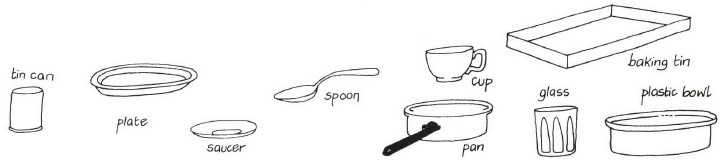
\includegraphics[width=12cm]{./img/vso/using-local-materials.jpg}
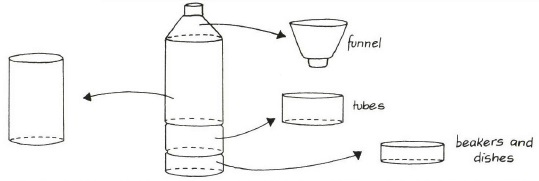
\includegraphics[width=12cm]{./img/vso/multi-purpose-bottle.jpg}
\end{center}

Below are common apparatus you might order from a laboratory supply company, 
and comments about which have good if not superior alternatives 
available in villages and towns. 
Given equal quality, 
it is generally better to use local materials, 
because these help connect classroom learning to students' lives.\\

The apparatus listed in this section are the following:

\begin{multicols}{3}

\begin{enumerate}
\item \nameref{sec:alligator-clips}
\item \nameref{sec:balance}
\item \nameref{sec:beakers}
\item \nameref{sec:blowpipe}
\item \nameref{sec:lightbulbs}
\item \nameref{sec:bunsen-burner}
\item \nameref{sec:burettes}
\item \nameref{sec:circuit-comp}
\item \nameref{sec:crucible}
%\item \nameref{sec:condenser}
\item \nameref{sec:containers}
\item \nameref{sec:deflagratingspoon}
\item \nameref{sec:delivery-tube}
\item \nameref{sec:drawing-board}
\item \nameref{sec:droppers}
\item \nameref{sec:electrodes}
\item \nameref{sec:electrode-holder}
%\item \nameref{sec:electrolytic-cell}
\item \nameref{sec:eureka-can}
\item \nameref{sec:filter-paper}
\item \nameref{sec:flasks}
\item \nameref{sec:funnel}
\item \nameref{sec:glass-blocks}
\item \nameref{sec:gloves}
\item \nameref{sec:goggles}
\item \nameref{sec:heatsources}
\item \nameref{sec:indicator}
\item \nameref{sec:iron-filings}
\item \nameref{sec:masses}
\item \nameref{sec:meascyl}
\item \nameref{sec:meter-rule}
\item \nameref{sec:microscope}
\item \nameref{sec:mirrors}
\item \nameref{sec:mortar-and-pestle}
\item \nameref{sec:nichrome-wire}
\item \nameref{sec:optical-pins}
\item \nameref{sec:pipettes}
\item \nameref{sec:pulleys}
\item \nameref{sec:resistors}
\item \nameref{sec:retort-stand}
\item \nameref{sec:scale-pan}
\item \nameref{sec:scalpels}
\item \nameref{sec:slide-cover-slip}
\item \nameref{sec:spatula}
\item \nameref{sec:spring-balance}
\item \nameref{sec:springs}
\item \nameref{sec:stoppers}
\item \nameref{sec:stopwatches}
\item \nameref{sec:testtubes}
\item \nameref{sec:test-tube-brush}
\item \nameref{sec:test-tube-holder}
\item \nameref{sec:test-tube-racks}
\item \nameref{sec:tripod-stands}
\item \nameref{sec:volumetric-glassware}
\item \nameref{sec:wash-bottle}
\item \nameref{sec:hotwaterbathes}
\item \nameref{sec:weights}
\item \nameref{sec:white-tiles}
\item \nameref{sec:wire}
\item \nameref{sec:wire-gauze}
\end{enumerate}

\end{multicols}

\begin{multicols}{2}

\section{Alligator Clips} \index{Alligator clips}
\label{sec:alligator-clips}
\vspace{-10pt}
\textbf{Use:} Connecting electrical components\\
\textbf{Materials:} Clothespins, aluminum foil, glue\\
\textbf{Procedure:} Glue aluminum foil around the clamping tips of a clothespin.

\section{Balance} \index{Beam balance! construction of}
\label{sec:balance}
\vspace{-10pt}
\textbf{Use:} Measuring mass\\
\textbf{Materials:} Ruler or wooden bar 30 cm $\times$ 2 cm, nails, razor/knife, string/wire, pen, 2 \nameref{sec:scale-pan}\\
\textbf{Procedure:} Find the balancing point of the ruler/wood block and mark it with a pen. Use a heated nail to make a hole through this point. Make notches at 5 cm intervals on either side of the center hole using a razor/knife to suspend scale pans. Use a string/wire tied through the center hole to suspend the balance.
\begin{center}
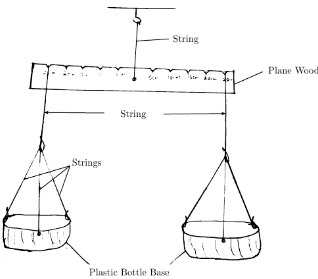
\includegraphics[width=0.45\textwidth]{./img/beam-balance.png}
\end{center}

\section{Beakers} \index{Beakers}
\label{sec:beakers}
\vspace{-10pt}
\textbf{Use:} To hold liquids, to heat liquids\\
\textbf{Materials:} Water bottles, jam jars, metal cans, knife\slash razor\\
\textbf{Procedure:} Take empty plastic bottles of different sizes. Cut them in half. The base can be used as a beaker. Jam jars made of glass, cut off metal cans and aluminum pots may be used when heating.\\
\textbf{Safety:} Glass containers may shatter if heated too much. Use standard laboratory equipment if extreme heating is needed.
\begin{center}
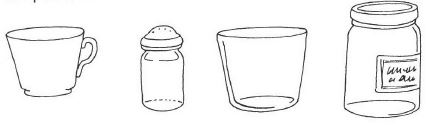
\includegraphics[width=8cm]{./img/vso/beakers.jpg}
\end{center} 

\section{Blowpipe} \index{Blowpipe}
\label{sec:blowpipe}
\vspace{-10pt}
\textbf{Use:} Increasing temperature of flames\\
\textbf{Materials:} Syringe needle, tube/straw/pen tube\\
\textbf{Procedure:} For sterilisation heat the needle
in open fire for a longer time before using it. A
drinking straw or a clean plastic tube can be
used as a connection to the mouth. 
\begin{center}
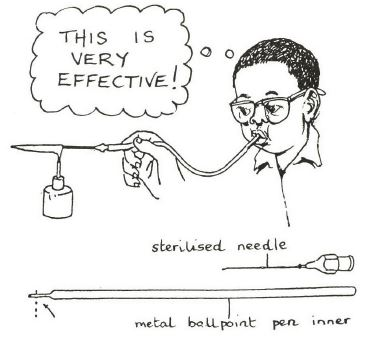
\includegraphics[width=0.4\textwidth]{./img/source/blowpipe.jpg}
\end{center} 

\section{Bulbs} \index{Bulbs}
\label{sec:lightbulbs}
\vspace{-10pt}
\textbf{Use:} Electrical circuits, diodes\\
\textbf{Materials:} Broken phone chargers, flashlights, other electronic devices\\
\textbf{Procedure:} Look for LEDs from broken items at hardware stores, local technicians, or small shops. 

\section{Bunsen Burner} \index{Bunsen burner|see{Heat sources}}
\label{sec:bunsen-burner}
See \nameref{sec:heatsources} (p.~\pageref{sec:heatsources}).

\section{Burettes} \index{Burettes! sources of}
\label{sec:burettes}
\vspace{-10pt}
\textbf{Use:} Titration\\
\textbf{Materials:} 10~mL syringes \\
\textbf{Procedure:} Use 10~mL disposable plastic syringes with 0.2~mL gradations. Students can estimate between the lines to at least 0.05~mL. If you must buy, buy plastic. Note that broken burettes can often be repaired -- see \nameref{cha:burettes} (p.~\pageref{cha:burettes}).

\section{Circuit Components} \index{Circuit components}
\label{sec:circuit-comp}
\vspace{-10pt}
\textbf{Use:} Building simple circuits, Ohm's Law, amplifier, wave rectifiers\\
\textbf{Materials:} Broken radio, computer, stereo, other electrical devices\\
\textbf{Procedure:} Remove resistors, capacitors, transistors, diodes, motors, wires, transformers, inductors, rheostats, pulleys, gears, battery holders, switches, speakers and other components from the devices. Capacitors tend to state their capacitance in microFarads on their bodies.

%\section{Condenser}
%\label{sec:condenser}
%Pass clear plastic tubing through a water bottle filled 
%with cold water and prevent leaks with super glue. 
%If your condenser is under-performing (i.e. 
%steam comes out), 
%coil the plastic tubing so a greater length is in the water. 
%If your condenser is still under-performing 
%or you plan to use it for longer period of time, 
%devise a way to keep changing water inside the water bottle 
%to keep it from getting too hot. 
%Or, 
%submerge this condenser in a trough of water. 
%You could even run the plastic tubing through the sides of a bucket.

\section{Containers} \index{Containers}
\label{sec:containers}
\vspace{-10pt}
\textbf{Use:} Measuring large volumes (100~mL -- 2~L) of solution, titration, storage\\
\textbf{Materials:} Plastic water bottles, jars, tin cans\\
\textbf{Procedure:} Identify the volume of useful marks on the bottles 
and combine to measure accurate volumes.
\begin{center}
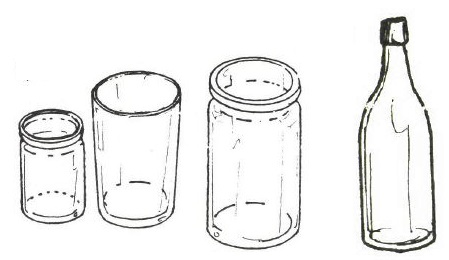
\includegraphics[width=0.4\textwidth]{./img/source/volumetric.jpg}
\end{center}

\section{Crucible} \index{Crucible}
\label{sec:crucible}
\vspace{-10pt}
\textbf{Use:} Heating substances at very high temperatures\\
\textbf{Materials:} 2 metal spoons, wire\\
\textbf{Procedure:} Place the material in one spoon and then wire 2 spoons together.
\begin{center}
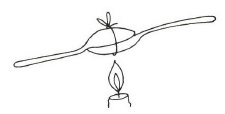
\includegraphics[width=0.4\textwidth]{./img/vso/crucible.jpg}
\end{center}

\section{Deflagrating Spoon} \index{Deflagrating spoon}
\label{sec:deflagratingspoon}
\vspace{-10pt}
\textbf{Use:} For heating chemicals to observe melting, decomposition, or other changes on heating\\
\textbf{Materials:} Metal spoons, galvanised wire, soda bottle cap\\
\textbf{Procedure:} Bend 30 cm of galvanised wire as shown. The wire should hold the bottle cap firmly.
\begin{center}
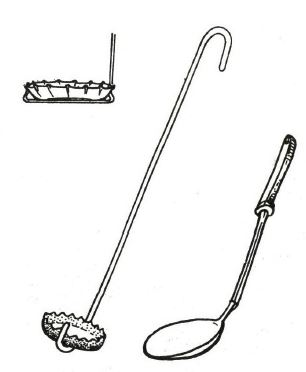
\includegraphics[width=0.3\textwidth]{./img/source/deflagrating-spoon.jpg}
\end{center}

\section{Delivery Tube} \index{Delivery tube}
\label{sec:delivery-tube}
\vspace{-10pt}
\textbf{Use:} Movement and collection of gases, capillary tubes, hydraulic press\\
\textbf{Materials:} Straws, pen tubes, IV tubing (giving sets) from a pharmacy, bicycle tubing
\begin{center}
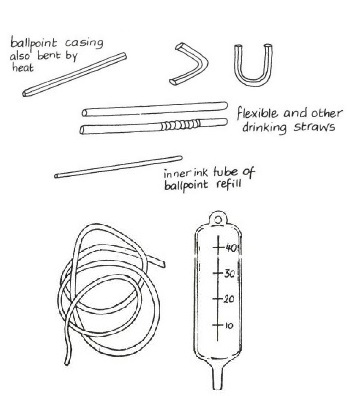
\includegraphics[width=0.45\textwidth]{./img/vso/tubes.jpg}
\end{center}

\section{Drawing Board} \index{Drawing board}
\label{sec:drawing-board}
\vspace{-10pt}
\textbf{Use:} Dissection, reflection, refraction of light\\
\textbf{Materials:} Thick cardboard

\section{Droppers} \index{Droppers}
\label{sec:droppers}
\vspace{-10pt}
\textbf{Use:} To transfer small amounts of liquid \\
\textbf{Materials:} 2 mL syringes, straws\\
\textbf{Procedure:} Take a syringe. Remove the needle to use as a dropper. Or insert a straw into a liquid and then plug the free end with a finger to remove a small amount and use as a dropper.

\section{Electrodes} \index{Electrodes}
\label{sec:electrodes}
\vspace{-10pt}
\textbf{Use:} Electrolysis
\begin{center}
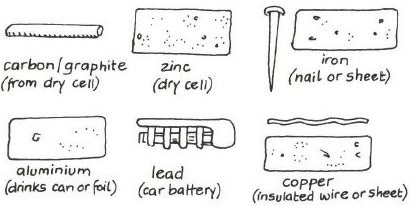
\includegraphics[width=0.45\textwidth]{./img/vso/electrodes.jpg}
\end{center}

\subsection{Graphite} \index{Graphite|see{Electrodes}}
\vspace{-6pt}
\textbf{Materials:} Old dry cell batteries\\
\textbf{Procedure:} Gently smash an old battery (D size) with a rock and pull out the electrode with pliers. DO NOT do this with alkaline batteries (most AA size) as they contain caustic liquids.
\subsection{Zinc} \index{Zinc|see{Electrodes}}
\vspace{-6pt}
\textbf{Materials:} New dry cell batteries\\
\textbf{Procedure:} Carefully open up a NEW dry cell (D size) battery by peeling back the steel shell and slicing the plastic inside. You should find a cylindrical shell of zinc metal. Empty out the black powder inside (manganese dioxide mixed with zinc chloride and ammonium chloride; wash your hands after) and keep the graphite electrode for another day. The zinc shell should then be cut into strips, scraped clean, and boiled in water or washed with soap to remove any residual chemicals that might affect your experiment.
\begin{center}
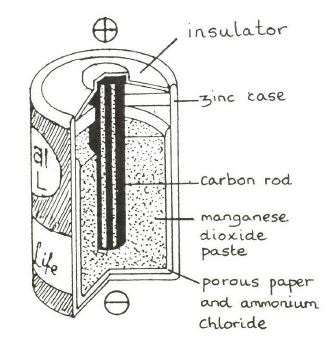
\includegraphics[width=0.4\textwidth]{./img/source/dry-cell.jpg}
\end{center}

\subsection{Iron} \index{Iron|see{Electrodes}}
\vspace{-6pt}
\textbf{Materials:} Ungalvanized nails from a hardware store
\subsection{Copper} \index{Copper|see{Electrodes}}
\vspace{-6pt}
\textbf{Materials:} Thick wire stripped of its insulation, also from a hardware store. Note that copper earthing rods have only a thin surface layer of copper these days.

%\section{Electrolytic cell}
%\label{sec:electrolytic-cell}
%Remove the plungers from two 10~mL syringes 
%and bore out the needle port with something sharp (knife, 
%thin pliers, 
%etc.). 
%Remove material gradually, 
%rotating the piece to ensure a circular cut. 
%When the hole is just big enough, 
%force through a graphite battery electrode 
%so 0.5-1~cm remains on the outside. 
%Twist the electrode during insertion to prevent it from snapping. 
%The gap should be air-tight, 
%but if the cut was too big or irregular 
%you can seal the holes with super glue. 
%Attach wires to the exposed part of the electrodes.
%
%To use the cell, 
%fill the tubes with your electrolyte solution 
%and place them wire end up in the cut off bottom of a large water bottle, 
%also filled with electrolyte solution. 
%Attach the wires to a power supply 
%(three or more 1.5~V dry cell batteries in series, 
%a 6~V motorcycle battery, 
%or a 12~V car battery) to start electrolysis. 
%The volume of gas produced at each electrode 
%may be measured by the gradations on the syringes, 
%and other products (copper metal plating, 
%iodine in solution) may be clearly observed.

\section{Electrode Holders} \index{Electrodes! holders}
\label{sec:electrode-holder}
\vspace{-10pt}
\textbf{Use:} Electrolysis\\
\textbf{Materials:} Clothes pins
\begin{center}
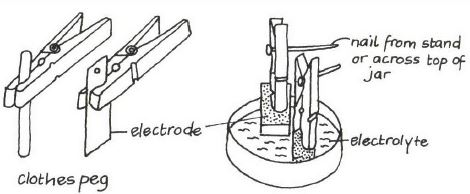
\includegraphics[width=0.49\textwidth]{./img/vso/electrode-holders.jpg}
\end{center}

\section{Eureka Can} \index{Eureka can}
\label{sec:eureka-can}
\vspace{-10pt}
\textbf{Use:} To measure volume of an irregular object, Archimedes' Principle, Law of Flotation\\
\textbf{Materials:} Plastic bottle, knife, Optional: super glue, straw, nail, candle\\
\textbf{Procedure:} Cut the top off of a 500 mL plastic bottle. Then cut a small strip at the top (1 cm wide by 3 cm long) and fold down to make a spout. Alternatively, heat a nail using a candle and poke a hole near the top of a cut off bottle. Super glue a straw so that it fits securely in the hole without leaking.
\begin{center}
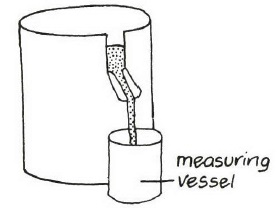
\includegraphics[width=5cm]{./img/vso/eureka-can.jpg}
\end{center}

\section{Filter Paper} \index{Filter paper}
\label{sec:filter-paper}
\vspace{-10pt}
\textbf{Use:} Filtration, separating mixtures, solutions\\
\textbf{Materials:} Cement bag paper, toilet paper, cloth
\begin{center}
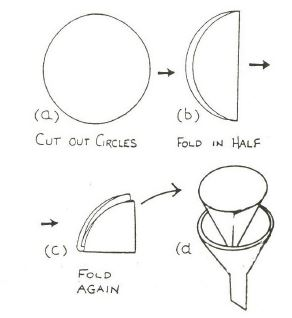
\includegraphics[width=0.4\textwidth]{./img/source/filter-paper.jpg}
\end{center}

\section{Flasks} \index{Flasks}
\label{sec:flasks}
\vspace{-10pt}
\textbf{Use:} Titrations, mixing solutions\\
\textbf{Materials:} Clean used liquor bottles, small water bottles\\
\textbf{Procedure:} When using these flasks for titrations, students must practice swirling enough that the solution remains well mixed. \\
\textbf{Safety:} When heating glass liquor bottles, make sure the cap is off.

\section{Funnel} \index{Funnel}
\label{sec:funnel}
\vspace{-10pt}
\textbf{Use:} To guide liquid or powder into a small opening\\
\textbf{Materials:} Empty water bottles, knife\\
\textbf{Procedure:} Take an empty water bottle and remove the cap. Cut it in half. The upper part of the bottle can be used as a funnel.  
\begin{center}
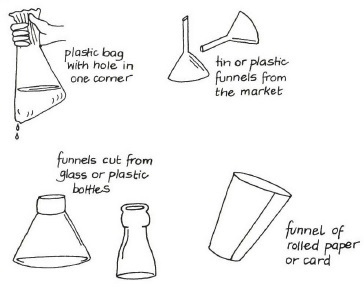
\includegraphics[width=0.49\textwidth]{./img/vso/funnels.jpg}
\end{center}

\section{Glass blocks} \index{Glass blocks}
\label{sec:glass-blocks}
\vspace{-10pt}
\textbf{Use:} Refraction of light\\
\textbf{Materials:} 8~mm - 15~mm slabs of glass\\
\textbf{Procedure:} Have a craftsman make rectangular pieces of glass with beveled edges, so students do not cut themselves. Glass blocks from a lab supply company are generally 15~mm thick. 8~mm and 10~mm glass is relatively common in towns. 12~mm and thicker glass exists though is even more difficult to find. Stack several pieces of thinner glass together and turn them on their edge.

\section{Gloves} \index{Gloves}
\label{sec:gloves}

\subsection{Latex gloves} 
\vspace{-6pt}
\textbf{Use:} First aid, when one has open cuts on hands, handling specimens. They are worthless to the chemist because they make the hands less agile and give the user a false sense of security.\\
\textbf{Safety:} Concentrated acids and organic chemicals burn straight through latex.

\subsection{Thick gloves} 
\vspace{-6pt}
\textbf{Use:} For working with organic solvents. Remember that the most dangerous organic solvents (benzene, carbon tetrachloride) should never be used in a school, with or without gloves. \\
\textbf{Materials:} Thick rubber gloves from village industry supply companies and some hardware stores\\
\textbf{Safety:} In general, avoid using chemicals that would make you want to wear gloves.

\section{Goggles} \index{Goggles}
\label{sec:goggles}
\vspace{-10pt}
\textbf{Use:} Handling concentrated acids\\
\textbf{Materials:} 1.5 L plastic water bottles, cardboard, sunglasses\\
\textbf{Procedure:} Cut a strip of plastic from a water bottle. Attach around your head with string or by using stiff cardboard as a frame. Goggles do not need to be impact resistant -- they just need to stand between hazardous chemicals and your eyes. 
\begin{center}
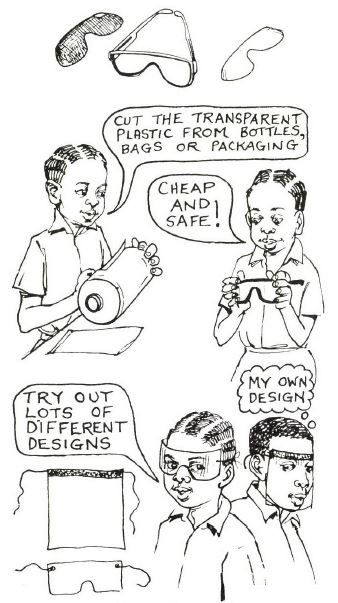
\includegraphics[width=0.4\textwidth]{./img/source/goggles.jpg}
\end{center}

\section{Heat Sources} \index{Heat sources}
\label{sec:heatsources}
\vspace{-10pt}
\textbf{Use:} Heating substances\\
\textbf{Materials:} Candles, kerosene stoves, charcoal burners, Motopoa (alcohol infused heavy oil), butane lighters, spirit burners, metal can, bottle caps \\
Motopoa provides the best compromise heat source - it is the easiest to use and safest heat source with locally available burners.\\
\textbf{Procedure:} Cut a metal can in half or use a bottle cap and add a small amount of Motopoa.\\
\textbf{Safety:} Always have available fire-fighting equipment that you know how to use. Remember that to put out a Bunsen burner safely, you need to turn off the gas.
\begin{center}
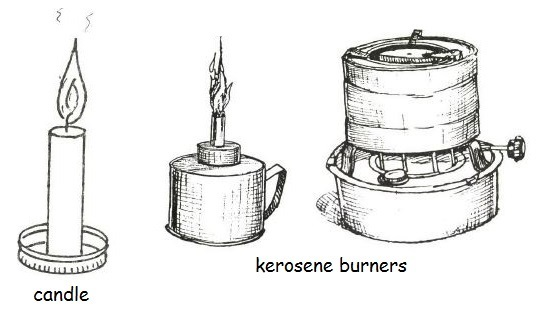
\includegraphics[width=0.49\textwidth]{./img/source/heat-sources.jpg}
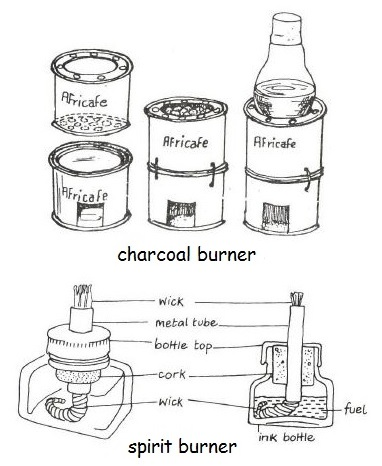
\includegraphics[width=0.49\textwidth]{./img/source/heat-sources-2.jpg}
\end{center}

\subsection{Heating Solutions} 
The ideal heat source has a high heat rate (Joules transferred per second), 
little smoke, 
and cheap fuel, i.e. Motopoa.
A charcoal stove satisfies all of these 
but takes time to light and requires relatively frequent re-fueling. 
Kerosene stoves have excellent heat rates but are smoky. 

\subsection{Heating Solids} 
The ideal heat source has a high temperature and no smoke, i.e. a Bunsen burner. 
For heating small objects for a short time (no more than 10-20 seconds), 
a butane lighter provides a very high temperature. 
Motopoa will provide a flame of satisfactory temperature 
for as long as necessary.

\subsection{Flame Tests} 
The ideal heat source has a high temperature 
and produces a non-luminous flame, i.e. a Bunsen burner. 
Motopoa is next best – hot and non-luminous. 
Spirit burners produce a non-luminous flame at much greater cost, 
unless methylated spirits are used as fuel 
in which case the flame is much cooler. 
A butane lighter produces a very hot flame of sufficient size 
and time for flame tests although the non-luminous region is small. 
Kerosene stoves will work for some salts.

\section{Indicators} \index{Indicators! sources of}
\label{sec:indicator}
\vspace{-10pt}
\textbf{Use:} Determine presence of acid or base, determine pH\\
\textbf{Materials:} Rosella leaves, hot water, bottle\\
\textbf{Procedure:} Place some coloured leaves into a bottle of warm water to extract the colour. Use a straw to drop onto solutions or prepare indicator paper by dipping thing strips into the coloured solution. Rosella turns red for acids and greenish blue for bases.
\begin{center}
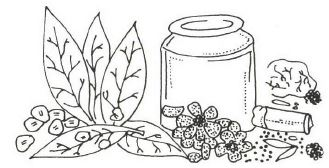
\includegraphics[width=0.4\textwidth]{./img/vso/making-indicators.jpg}
\end{center}

\section{Iron Filings} \index{Iron filings}
\label{sec:iron-filings}
\vspace{-10pt}
\textbf{Use:} To map magnetic fields\\
\textbf{Materials:} Steel wool / Iron wool used for cleaning pots\\
\textbf{Procedure:} Rub some steel wool between your thumb and fingers.  The small pieces that fall are iron filings.  Collect them in a matchbox or other container to use again.

\section{Masses} \index{Masses|see{Weights}}
\label{sec:masses}
See \nameref{sec:weights} (p.~\pageref{sec:weights}).

\section{Measuring Cylinder} \index{Measuring cylinder}
\label{sec:meascyl}
\vspace{-10pt}
\textbf{Use:} Measuring volume\\
\textbf{Materials:} Plastic bottles of different sizes, syringes (10 mL - 50 mL), fluorescent light tubes, marker pen, ruler, bucket of water\\
\textbf{Procedure:} Using the syringe, transfer a known volume of water from the bucket to the empty bottle. Use the marker pen to mark the level of water on the bottle. Repeat for a range of volumes, using a ruler to complete the scale. 
\begin{center}
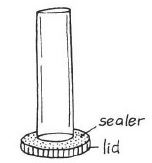
\includegraphics[width=0.2\textwidth]{./img/vso/meas-cyl.jpg}
\end{center}

\section{Metre Rule} \index{Metre rule}
\label{sec:meter-rule}
\vspace{-10pt}
\textbf{Use:} Measuring length\\
\textbf{Materials:} Slabs of wood, ceiling board, permanent pen\\
\textbf{Procedure:} Buy one, take it and a permanent pen to a carpenter, and leave with twenty. Measure each new one to the original rule to prevent compounding errors.

\section{Microscope} 
\label{sec:microscope}
See \nameref{cha:microscopy} (p.~\pageref{cha:microscopy}).

\section{Mirrors} \index{Mirrors}
\label{sec:mirrors}

\subsection{Plane Mirrors} \index{Mirrors! plane}
\vspace{-6pt}
\textbf{Use:} Microscope, Laws of Reflection\\
\textbf{Materials:} piece of thin glass, kibatari, super glue, small wooden blocks 

\emph{Optional}: Small pieces of mirror glass are cheap or free at a glass cutter's shop\\
\textbf{Procedure:} Light the kibatari so that it creates a lot of smoke.  Pass one side of the glass repeatedly over the kibatari until that side is totally black.  The other side acts as a mirror. Super glue to small wooden blocks to stand upright.

\subsection{Curved Mirrors} \index{Mirrors! curved}
\vspace{-6pt}
\textbf{Use:} Curved mirror practicals\\
\textbf{Materials:} Spoons\\
\textbf{Procedure:} Inside surface is a concave mirror; back surface is a convex mirror.
\begin{center}
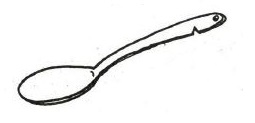
\includegraphics[width=0.2\textwidth]{./img/source/spoon.jpg}
\end{center}

\section{Mortar and Pestle} \index{Mortar and pestle}
\label{sec:mortar-and-pestle}
\vspace{-10pt}
\textbf{Use:} To powder chemicals\\
\textbf{Materials:} 2 metal spoons, glass bottle\\
\textbf{Procedure:} Place chemicals between two nested metal spoons and grind down. 
Alternatively, crush chemicals on a sheet of paper by pressing on them with the bottom of a glass bottle.
\begin{center}
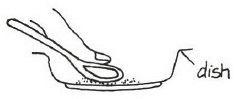
\includegraphics[width=5cm]{./img/vso/mortar-pestle.jpg}
\end{center}

\section{Nichrome Wire} \index{Wire! nichrome}
\label{sec:nichrome-wire}
For flame tests in chemistry, 
you can use a steel wire thoroughly scraped clean with iron or steel wool. 
For physics experiments, 
see \nameref{sec:wire} (p.~\pageref{sec:wire}).

\section{Optical Pins} \index{Optical pins}
\label{sec:optical-pins}
\vspace{-10pt}
\textbf{Use:} Compass needles, making holes, dissection, mirror practicals\\
\textbf{Materials:} Office pins, sewing needles, needles from syringes

\section{Pipettes} \index{Pipettes}
\label{sec:pipettes}
\vspace{-10pt}
\textbf{Use:} Transferring small amounts of liquid\\
\textbf{Materials:} Disposable plastic syringes (1, 2, 5, 10, 20, 25, 30 and 50 mL sizes)\\
\textbf{Procedure:} Suck first 1~mL of air and then put the syringe into the solution to suck up the liquid. There should be a flat meniscus under the layer of air.\\
\textbf{Safety:} Avoid standard pipettes to eliminate danger of mouth pipetting.
\begin{center}
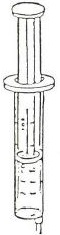
\includegraphics[width=0.1\textwidth]{./img/source/syringe.jpg}
\end{center}

\section{Pulleys} \index{Pulleys}
\label{sec:pulleys}
\vspace{-10pt}
\textbf{Use:} Simple machines\\
\textbf{Materials:} Bent nail, twisted wire, thread reel, water bottle, string, coat hanger\\
\textbf{Procedure:} Cut off the top of a water bottle just below the lip where the top screws on. Run string or stiff wire through the centre to hang from a table or chair.
\begin{center}
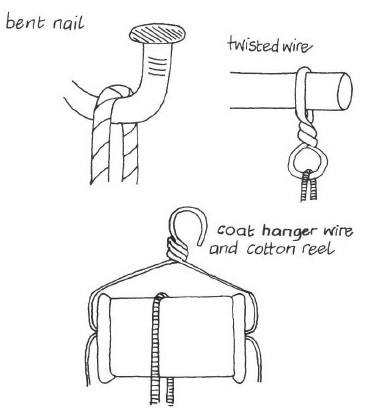
\includegraphics[width=0.4\textwidth]{./img/vso/pulleys.jpg}
\end{center}

\section{Resistors} \index{Resistors}
\label{sec:resistors}
\vspace{-10pt}
\textbf{Use:} Electrical components\\
\textbf{Materials:} Old radios, circuit boards, soldering iron\\
\textbf{Procedure:} Remove resistors from old radios and circuit boards by melting the solder with a soldering iron or a stiff wire heated by a charcoal stove. If you need to know the ohms, the resistors tell you. Each has four strips (five if there is a quality band) and should be read with the silver or gold strip for tolerance on the right. Each color corresponds to a number:\\[10pt]

\begin{tabular}{lll}
black = 0 & yellow = 4 & violet = 7\\
brown = 1 & green = 5 & gray = 8\\
red = 2 & blue = 6 & white = 9\\
orange = 3 & & \\[10pt]
\end{tabular} 

\noindent and additionally for the third stripe: gold = -1 and silver = -2. \\

\noindent The first two numbers should be taken as a two digit number, so green-violet would be 57, red-black 20, etc. The third number should be taken as the power of ten (a $ 10^{n} $ term), so red-orange-yellow would be $ 23 \times 10^{4} = 230000 $, red-brown-black would be $ 21 \times 10^{0} = 21 $ and blue-gray-silver would be $ 68 \times 10^{-2} = 0.68 $. The unit is always ohms. The fourth and possibly fifth bands may be ignored.

\section{Retort Stand} \index{Retort stand}
\label{sec:retort-stand}
\vspace{-10pt}
\textbf{Use:} To hold springs, burettes, pendulums or other objects\\
\textbf{Materials:} Filled 1.5 L water bottle, straight bamboo stick, tape, marker\\
\textbf{Procedure:} Tape the bamboo stick across the top of the water bottle so that it reaches out ~20 cm to one side. Attach a small clamp if required or hang the object directly from the bamboo stick.

Alternatively, place a 1~cm piece of reinforcing rod in a paint can full of wet cement and let it dry. Then attach a boss head and clamp.

\section{Scale Pans} \index{Scale pans}
\label{sec:scale-pan}
\vspace{-10pt}
\textbf{Use:} Beam balance\\
\textbf{Materials:} Plastic bottle, cardboard box, string\\
\textbf{Procedure:} Cut off the bottom of a plastic bottle or cardboard box. Poke 3 or more holes near the top and tie string through each hole. Join strings and tie at the top to hang from a single point.
\begin{center}
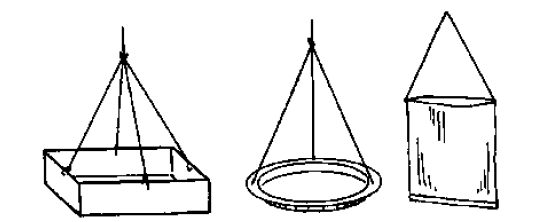
\includegraphics[width=8cm]{./img/source/scale-pans.png}
\end{center}

\section{Scalpels} \index{Scalpels}
\label{sec:scalpels}
\vspace{-10pt}
\textbf{Use:} Dissection\\
\textbf{Materials:} Razor blades, tongue depressors, super glue\\
\textbf{Procedure:} Add a handle by gluing a tongue depressor on either side of the razor blade. Hold together with a rubber band until dry.\\
\textbf{Safety:} Dull blades should be discarded. Because students need to apply more pressure when using them, there is a greater risk of slipping and thus of cuts. Sharp tools are much safer. 
\begin{center}
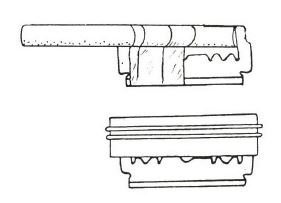
\includegraphics[width=0.4\textwidth]{./img/source/scalpel.jpg}
\end{center}

\section{Slides and Cover Slips} \index{Slides} \index{Cover slips}
\label{sec:slide-cover-slip}
\vspace{-10pt}
\textbf{Use:} Microscopy\\
\textbf{Materials:} Small pieces of glass, stiff plastic\\
\textbf{Procedure:} Small piece of glass provides a slide for mounting the
specimen. Cover slips can be made
from thin (but stiff) transparent plastic from
display packing or bottles. Cut into small squares or circles.
\begin{center}
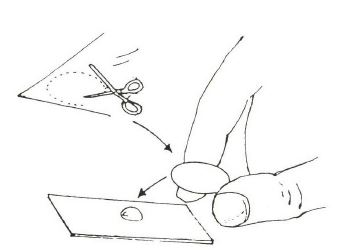
\includegraphics[width=0.4\textwidth]{./img/source/slide-cover-slip.jpg}
\end{center}

\section{Spatula} \index{Spatula}
\label{sec:spatula}
\vspace{-10pt}
\textbf{Use:} Transferring salts\\
\textbf{Materials:} Stainless steel spoons\\
\textbf{Procedure:} Use the handle end to remove salts from containers.\\
\textbf{Safety:} Clean all metal tools promptly after using with hydroxide, 
potassium manganate (VII), 
or manganese (IV) oxide. 
If the spoon corrodes, scrape with another spoon or steel wool.
\begin{center}
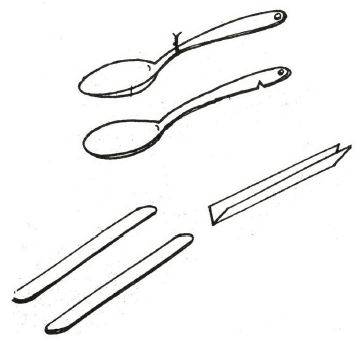
\includegraphics[width=0.4\textwidth]{./img/source/spatula.jpg}
\end{center}

\section{Spring Balance} \index{Spring balance}
\label{sec:spring-balance}
\textbf{Use:} To measure force applied on an object\\
\textbf{Materials:} Strip of cardboard, rubber band, 2 paper clips, staple pin, pen\\
\textbf{Procedure:} Cut a rubber band and fix one end to the top of a cardboard strip using a staple pin. (A stronger rubber band allows for a greater range of forces to measure.) Attach one paper clip near the top as a pointer. Attach the other paper clip as a hook at the bottom of the rubber band. Calibrate the spring balance using known masses. Write the equivalent force in Newtons on the cardboard. (A 1~g mass has a weight of 0.01 N, 100 g has a weight of 1 N, etc.)
\begin{center}
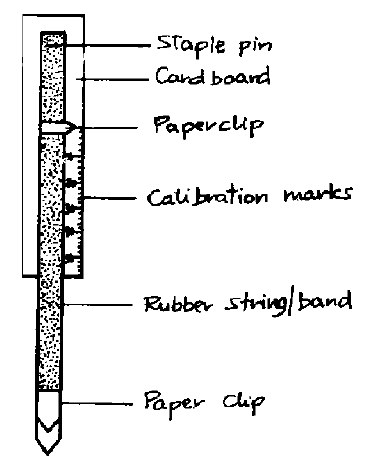
\includegraphics[width=0.4\textwidth]{./img/source/spring-balance.png}
\end{center}

\section{Springs} \index{Springs}
\label{sec:springs}
\vspace{-10pt}
\textbf{Use:} Hooke's Law, potential energy, work, spring balance\\
\textbf{Materials:} Springs from hardware stores, bike stores, junk merchants in markets, window blinds; stiff wire; rubber bands; strips of elastic\\
\textbf{Procedure:} Remove plastic covering if necessary and cut to a desired length (~5 cm). Alternatively wind a stiff wire around a marker pen or use rubber bands or elastic from a local tailor.

\section{Stoppers} \index{Stoppers}
\label{sec:stoppers}
\vspace{-10pt}
\textbf{Use:} To cover the mouth of a bottle, hold a capillary tube\\
\textbf{Materials:} Rubber from old tires or sandals, cork, plastic bottle cap, pen tube, super glue\\
\textbf{Procedure:} Cut a circular piece of rubber.  If the stopper is being used to hold a capillary tube, a hole can be melted in a plastic cap or rubber stopper. Alternatively, super glue a pen tube to a plastic bottle cap and connect to rubber tubing.
\begin{center}
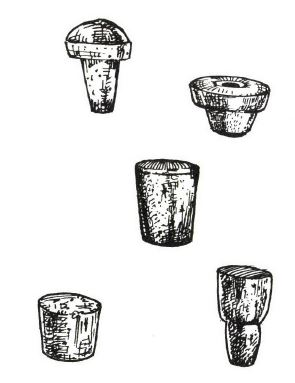
\includegraphics[width=0.3\textwidth]{./img/source/stoppers.jpg}
\end{center}

\section{Stopwatches} \index{Stopwatches}
\label{sec:stopwatches}
\vspace{-10pt}
\textbf{Use:} Simple pendulum, velocity, acceleration\\
\textbf{Materials:} Athletic and laboratory stopwatches from markets, digital wristwatches

\section{Test Tubes} \index{Test tubes}
\label{sec:testtubes}

\subsection{Plastic Test Tubes}
\vspace{-6pt}
\textbf{Use:} To heat materials without a direct flame, to combine solutions\\
\textbf{Materials:} 10~mL syringes, matches\\
\textbf{Procedure:} Remove the needle and plunger from 10~mL syringes. Heat the end of the shell with a match until it melts. Press the molten end against a flat surface (like the end of the plunger) to fuse it closed. If the tube leaks, fuse it again. Test tubes made this way may be heated in a water bath up to boiling, hot enough for most experiments.
\begin{center}
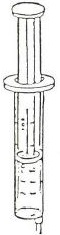
\includegraphics[width=0.1\textwidth]{./img/source/syringe.jpg}
\end{center}

\subsection{For Thermal Decomposition} 
See \nameref{sec:deflagratingspoon} (p.~\pageref{sec:deflagratingspoon}).

\section{Test Tube Brush} \index{Test tubes! brushes}
\label{sec:test-tube-brush}
\vspace{-10pt}
\textbf{Use:} Cleaning test tubes\\
\textbf{Materials:} Sisal, wire\\
\textbf{Procedure:} Twist the wire around the sisal as shown or put a little sand in the test tube as an abrasive.
\begin{center}
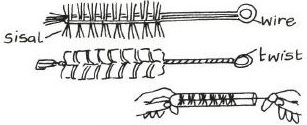
\includegraphics[width=0.45\textwidth]{./img/vso/test-tube-brush.jpg}
\end{center}

\section{Test Tube Holder / Tongs} \index{Test tubes! holders}
\label{sec:test-tube-holder}
\vspace{-10pt}
\textbf{Use:} To handle test tubes\\
\textbf{Materials:} Wooden clothespins, stiff wire, strip of paper or cloth\\
\textbf{Procedure:} Use clothespins or stiff wire for prolonged heating, or strips of paper or cloth for short-term heating.
\begin{center}
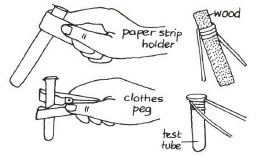
\includegraphics[width=0.45\textwidth]{./img/vso/test-tube-holder.jpg}
\end{center}

\section{Test Tube Racks} \index{Test tubes! racks}
\label{sec:test-tube-racks}
\vspace{-10pt}
\textbf{Use:} To hold test tubes vertically in place\\
\textbf{Materials:} Wire grid from local gardening store, styrofoam block, plastic bottle, sand, knife\\
\textbf{Procedure:} Fold a sheet of wire grid to make a table; punch holes in a piece of styrofoam; cut a plastic bottle in half and fill it with sand to increase stability. Or cut a plastic bottle along its vertical axis and rest the two cut edges on a flat surface. Cut holes into it for the test tubes.
\begin{center}
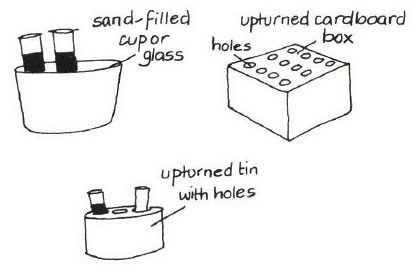
\includegraphics[width=0.45\textwidth]{./img/vso/test-tube-rack.jpg}
\end{center}

\section{Tripod Stands} \index{Tripod stands}
\label{sec:tripod-stands}
\vspace{-10pt}
\textbf{Use:} For supporting containers above heat sources, for elevating items\\
\textbf{Materials:} Stiff wire, metal rods, tin can\\
\textbf{Procedure:} Join bent pieces of thick wire together. Or cut the sides of a tin can to leave 3 legs.
\begin{center}
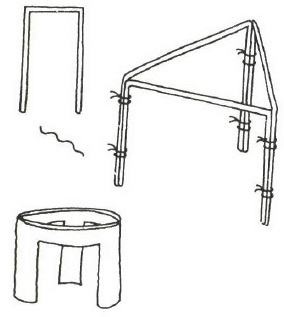
\includegraphics[width=5cm]{./img/vso/tripod-stand.jpg}
\end{center}

\section{Volumetric ``Glass''ware} \index{Volumetric glassware|see{Containers}}
\label{sec:volumetric-glassware}
See \nameref{sec:containers} (p.~\pageref{sec:containers}).

\section{Wash Bottle} \index{Wash bottle}
\label{sec:wash-bottle}
\vspace{-10pt}
\textbf{Use:} Washing hands after experiments\\
\textbf{Materials:} Water bottle, detergent, needle\\
\textbf{Procedure:} Put a hole in the cap of a water bottle using a syringe needle. 

\section{Water Bath} \index{Water bath}
\label{sec:hotwaterbathes}
\vspace{-10pt}
\textbf{Use:} To heat substances without using a direct flame\\
\textbf{Materials:} \nameref{sec:heatsources}, water, cooking pot\\
\textbf{Procedure:} Bring water to a boil in a small aluminum pot, then place the test tubes in the water to heat the substance inside the test tube. Prevent test tubes from falling over by clamping with clothespins or placing parallel wires across the container.
\begin{center}
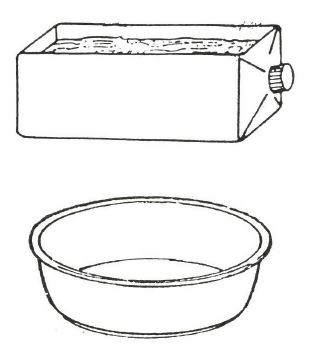
\includegraphics[width=0.4\textwidth]{./img/source/trough.jpg}
\end{center}

\section{Weights} \index{Weights}
\label{sec:weights}

\subsection{Crude Weights}
\vspace{-6pt}
\textbf{Use:} Concept of units, mass, weight\\
\textbf{Materials:} Batteries, coins, glass marbles from town, etc. \\
\textbf{Procedure:} Use objects of unknown mass to create new units and impart the concept of unit measure.

\subsection{Adding Weight in Known Intervals} 
\vspace{-6pt}
\textbf{Use:} Hooke's Law practical\\
\textbf{Materials:} Water bottles, syringe\\
\textbf{Procedure:} Consider ``zero added mass'' the displacement of the pan with an empty water bottle. Then add masses of water in g equal to their volumes in mL (e.g. 50 mL = 50 g).

\subsection{Precise Weights}
\vspace{-6pt}
\textbf{Materials:} Plastic bags, sand, stones, 250 mL water bottles (all identical), tape, pen\\
\textbf{Procedure:} 
Use a beam balance and known masses at a market or nearby school to measure exact masses of bags of sand or stones.  Use a marker pen to mark the masses on the bags. 

If using water, use a beam balance from a nearby school to measure the exact mass of an empty water bottle. Add a volume of water in mL equal to the mass in g needed to reach a desired total mass. (The density of water is 1.0 g/mL.) This can be done precisely by using a plastic syringe. Label the bottle with tape and a pen.

\section{White Tiles} \index{White tiles}
\label{sec:white-tiles}
\vspace{-10pt}
\textbf{Use:} Titration\\
\textbf{Materials:} White paper\\
\textbf{Procedure:} If students are using syringes as burettes, they can also hold their flask up against a white wall.

\section{Wire} \index{Wire}
\label{sec:wire}

\subsection{Connecting Wires} \index{Wire! connecting}
\vspace{-6pt}
\textbf{Use:} Connecting circuit components, current electricity\\
\textbf{Materials:} Speaker wire, knife\\
\textbf{Procedure:} Speaker wire can be found at any hardware store or taken from old appliances - the pairs of colored wires brained together. Strip using a knife, scissors or a wire stripper.
\begin{center}
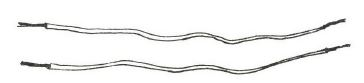
\includegraphics[width=0.4\textwidth]{./img/source/wire.jpg}
\end{center}

\subsection{Specific Gauge Wire} \index{Wire! specific gauge}
\vspace{-6pt}
\textbf{Use:} Electrical components, motors, transformers, simple generators\\
\textbf{Materials:} Copper wire without plastic covering (transformer wire), knife\slash scissors, matches\\
\textbf{Procedure:} Scrape or burn off the insulating varnish at any points you wish to make electrical contact. 
These wires come in a variety of diameters (gauges). A useful chart for converting diameter to gauge may be found at \url{http://www.dave-cushman.net/elect/wiregauge.html}. If the wire is sold by weight, 
you can find the length if you know the diameter - the density of copper metal at room temperature is 8.94~g/cm$^{3}$. For example, with 0.375~mm wire, 250~g is about 63 metres.

\section{Wire Gauze} \index{Wire gauze}
\label{sec:wire-gauze}
\vspace{-10pt}
\textbf{Use:} Placing objects over heat\\
\textbf{Materials:} Tin can lid\\
\textbf{Procedure:} Poke holes in a tin can lid.
\begin{center}
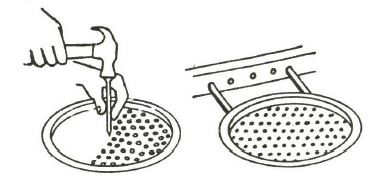
\includegraphics[width=0.4\textwidth]{./img/source/wire-gauze.jpg}
\end{center}

\end{multicols}
\chapter{Sources of Chemicals}
\label{cha:sourcesofchemicals}
The following is a list of most of the chemicals 
used in science laboratories. 
For each we note local sources of these chemicals, 
low cost industrial sources of these chemicals, 
methods to manufacture these chemicals at your school, 
and/or functional alternatives to these chemicals. 
We also list information like other names, 
common uses, 
and hazards. 
Finally, 
we include descriptions of many of the compounds 
and confirmatory tests for some to assist 
with identification of unlabelled chemicals. 
For more information on this, 
see \nameref{cha:unknownchemicals}.

Chemicals are generally listed alphabetically by IUPAC name, 
although many compounds are also cross listed by their common name (e.g. 
acetone (common) / propanone (IUPAC)).

\section{2-methylpropanol}
\label{sec:methylpropanol}
Formula: \ce{(CH3)2CHCH2OH}\\
Other names: isobutanol\\
Description: clear liquid less dense than water, 
alcohol smell similar to isopropanol (American rubbing alcohol)\\
Use: organic solvent for distribution (partition) experiments\\
Alternative: paint thinner or kerosene\\
Note: if ordering this chemical for the national exam, 
make sure that you get this chemical exactly. 
Other compounds, 
e.g. 
\ce{CH3CH2CH2(OH)CH3} (butan-2-ol) are sometimes sold 
as ‘isobutanol’ but do not work the same way.

\section{Acetaldehyde}
See \nameref{sec:ethanal}.

\section{Acetic acid}
See \nameref{sec:ethanoic}.

\section{Acetone}
See \nameref{sec:propanone}.

\section{Alum}
See \nameref{sec:potalsulf}.

\section{Ammonia solution}
\label{sec:ammoniasol}
Formula: \ce{NH3}$_{(aq)}$\\
Other names: ammonium hydroxide, 
ammonium hydroxide solution\\
Description: clear liquid less dense than water, 
completely miscible in water, 
strong biting smell similar to old urine\\
Use: qualitative analysis, various experiments\\
Source: released from an aqueous mixture of ammonium salt and hydroxide, 
for example calcium ammonium nitrate and sodium hydroxide. 
The gas can be trapped and dissolved in water.\\
Alternative: to distinguish between zinc and lead cations, 
add dilute sulfuric acid dropwise. 
The formation of a white precipitate -- lead sulfate -- confirms lead.
Note: ammonia solution also is called ammonium hydroxide 
because ammonia undergoes autoionization to form ammonium and hydroxide ions. 
Just like water, 
there is an equilibrium concentration of the ions in an ammonia solution.

\section{Ammonium dichromate}
Formula: \ce{(NH3)2Cr2O7}\\
Description: orange crystals soluble in water\\
Use: qualitative analysis (identification of sulfur dioxide gas)\\
Hazard: toxic, 
water pollutant\\
Alternative: make ammonium/potassium dichromate paper tests. 
Many can be made from a single gram of ammonium/potassium dichromate.

\section{Ammonium hydroxide solution}
See \nameref{sec:ammoniasol}.

\section{Ammonium carbonate, chloride, and nitrate}
Use: qualitative analysis, 
preparation of ammonia\\
Alternative: to teach the identification 
and confirmation of ammonium salts and to prepare ammonia, 
use calcium ammonium nitrate.

\section{Ammonium sulphate}
Formula: \ce{(NH4)2SO4}
Other name: sulphate of ammonia
Description: white crystals
Use: qualitative analysis, preparation of ammonia\\
Source: fertilizer

\section{Ammonium thiocyanate}
Formula: \ce{NH4SCN}\\
Use: confirmation of iron III in qualitative analysis\\
Alternative: addition of sodium ethanoate 
should also produce a blood red solution; 
additionally, 
the test is unnecessary, 
as iron III is also the only chemical 
that will produce a red/brown precipitate with sodium hydroxide solution 
or sodium carbonate solution.

\section{Ascorbic acid}
Other names: vitamin C\\
Formula: \ce{C6H7O7}\\
Description: white powder, 
but pharmacy tablets often colored\\
Confirm: aqueous solution turns blue litmus red 
AND decolorizes dilute iodine or potassium permanganate solution\\
Use: all-purpose reducing agent, 
may substitute for sodium thiosulfate in redox titrations, 
removes iodine and permanganate stains from clothing\\
Source: pharmacies

\section{Barium chloride and barium nitrate}
Use: confirmatory test for sulfate in qualitative analysis\\
Description: white crystals\\
Hazard: toxic, 
water pollutant\\
Alternative: lead nitrate will precipitate lead sulfate – 
results identical to when using barium

\section{Boric acid}
Formula: \ce{H3BO3}\\
Description: white powder\\
Confirm: deep green flame color\\
Use: flame test demonstrations, preparation of sodium borate\\
Source: village industry supply shops, industrial chemical

\section{Benedict's solution}
\label{sec:benedict}
Description: bright blue solution\\
Confirm: gives orange precipitate when boiled with glucose\\
Use: food tests (test for reducing and non reducing sugars)\\
Hazard: copper is poisonous\\
Manufacture: combine 5 spoons of sodium carbonate, 
3 spoons of citric acid, 
and one spoon of copper sulfate in half a liter of water. 
Shake until everything is fully dissolved.

\section{Benzene}
Formula: \ce{C6H6}\\
Description: colorless liquid insoluble in water\\
Use: all purpose organic solvent\\
Hazard: toxic, 
highly carcinogenic – see section on Dangerous Chemicals\\
Alternative: toluene is safer but for most solvent applications 
kerosene is equally effective and far less expensive.

\section{Butane}
Formula: \ce{C4H10}\\
Source: the fluid in gas lighters is butane under pressure; 
liquid butane may be obtained at normal pressure with the help of a freezer

\section{Calcium ammonium nitrate}
Other names: \ce{CAN}\\
Description: small pellets, 
often with brown coating; 
endothermic heat of solvation\\
Use: low cost ammonium salt for teaching qualitative analysis; 
not as useful for teaching about nitrates 
as no red/brown gas released when heated. 
May be used for the preparation of ammonia and sodium nitrate.\\
Source: agricultural shops (fertilizer)\\

\section{Calcium carbonate}
Formula: \ce{CaCO3}\\
Description: white powder, 
insoluble in water
Confirm: brick red flame test and acid causes effervescence\\
Use: demonstration of reactivity of carbonates, 
rates of reaction, 
qualitative analysis\\
Source: coral rock, 
sea shells, 
egg shells, 
limestone, 
marble, 
white residue from boiling water\\
Local manufacture: prepare a solution of aqueous calcium 
from either calcium ammonium nitrate or calcium hydroxide 
and add a solution of sodium carbonate.\\ 
Calcium carbonate will precipitate and may be filtered and dried.

\section{Calcium chloride and calcium nitrate}
Description: highly deliquescent colorless crystals 
(poorly sealed containers often become thick liquid)\\
Use: qualitative analysis salts, 
drying agents\\
Alternatives (qualitative analysis): 
to practice identification of the calcium cation, 
use calcium sulfate; 
to practice identification of the chloride anion, 
use sodium chloride\\
Alternative (drying agent): sodium sulfate

\section{Calcium hydroxide}
Formula: \ce{Ca(OH)2}\\
Other names: quicklime\\
Local name: \textit{chokaa}\\
Description: white to off white powder, 
sparingly soluble in water\\
Use: dissolve in carbonate-free water to make limewater\\
Source: building supply shops\\
Alternative: add a small amount of cement to water, 
let settle, 
and decant the clear solution; 
this is limewater.

\section{Calcium oxide}
Formula: \ce{CaO}\\
Other names: lime\\
Use: reacts with water to form calcium hydroxide, 
thus forming limewater\\
Source: cement is mostly calcium oxide

\section{Calcium sulfate}
Formula: \ce{CaSO4\cdot} 2\ce{H2O}\\
Other names: gypsum, 
plaster of Paris\\
Description: white powder, 
insoluble in cold water but soluble in hot water\\
Use: qualitative analysis\\
Source: building supply companies (as gypsum powder)

\section{Carbon (amorphous)}
Source: soot, 
charcoal (impure)

\section{Carbon (graphite)}
\label{sec:carbongraphite}
Use: element, \\
inert electrodes for chemistry and physics
Source: dry cell battery electrodes, 
pencil cores (impure)

\section{Carbon dioxide}
Preparation: react an aqueous weak acid 
(citric acid or ethanoic acid) with a soluble carbonate 
(sodium carbonate or sodium hydrogen carbonate)

\section{Carbon tetrachloride}
See \nameref{sec:tetrachloromethane}.

\section{Chloroform}
See \nameref{sec:trichloromethane}.

\section{Citric acid}
Formula: \ce{C6H8O7} =  \ce{CH2(COOH)COH(CHOOH)CH2COOH}\\
Local name: \textit{unga wa ndimu}\\
Description: white crystals soluble in water, 
endothermic heat of solvation\\
Use: all purpose weak acid, 
volumetric analysis, 
melting demonstration, 
preparation of carbon dioxide, 
manufacture of Benedict's solution\\
Hazard: acid – keep out of eyes!\\
Source: markets (sold as a spice), 
supermarkets

\section{Cobalt chloride}
Use: test for water (hydrated cobalt chloride is pink)\\
Hazard: cobalt is poisonous\\
Alternative: white anhydrous copper sulfate turns blue when hydrated

\section{Copper}
\label{sec:copper}
Use: element, 
preparation of copper sulfate, 
electrochemical reactions\\
Description: dull red/orange metal\\
Source: electrical wire -- e.g. 
2.5~mm gray insulated wire has 50~g of high purity copper per meter.\\
Note: modern earthing rods are only copper plated, 
and thus no longer a good source of copper

\section{Copper carbonate}
Formula: \ce{CuCO3}\\
Description: light blue powder\\
Confirm: blue/green flame test and dilute acid causes effervescence\\
Use: qualitative analysis, 
preparation is a demonstration of double decomposition\\
Hazard: powder may be inhaled; 
copper is poisonous\\
Local manufacture: prepare solutions of copper sulfate 
and sodium carbonate and mix them. 
Copper carbonate will precipitate 
and may be purified by filtration and drying.

\section{Copper chloride and copper nitrate}
Description: blue-green (copper chloride) 
and deep blue (copper nitrate) salts \\
Use: qualitative analysis\\
Alternatives: for practice identifying the copper cation, 
use copper sulfate; 
for practice identifying the chloride anion, 
use sodium chloride

\section{Copper oxygen chloride}
Formula: \ce{Cu2OCl}\\
Other names: copper oxychloride, 
blue copper\\
Description: light blue powder\\
Hazard: powder may be inhaled; 
copper is poisonous\\
Source: agricultural shops (fungicide)

\section{Copper sulfate}
Formula: \ce{CuSO4} (anhydrous), 
\ce{CuSO4\cdot} 5\ce{H2O} (pentahydrate)\\
Local name: \textit{mlutuluru}\\
Description: white (anhydrous) or blue (pentahydrate) crystals\\
Confirm: blue/green flame test 
and aqueous solution gives a white precipitate 
when mixed with lead or barium solution\\
Use: qualitative analysis, 
demonstration of the reactivity series, 
manufacture of Benedict's solution, 
test for water\\
Source: imported ``local'' medicine (manufactured in India).\\ 
Local manufacture: Electrolyze dilute (1-2~M) sulfuric acid 
with a copper anode and inert (e.g. 
graphite) cathode. 
Evaporate final solution until 
blue crystals of copper sulfate pentahydrate precipitate. 
To prepare anhydrous copper sulfate from copper sulfate pentahydrate, 
gently heat until the blue color has faded. 
Strong heating will irreversibly form black copper oxide. 
Store anhydrous copper sulfate in an air-tight container -- 
otherwise atmospheric moisture will reform the pentahydrate.

\section{Dichloromethane}
Formula: \ce{CH2Cl2}\\
Use: organic solvent for distribution (partition) experiments\\
Hazard: toxic by inhalation and ingestion (mouth pipetting) 
and by absorption though skin\\
Alternative: paint thinner or kerosene, 
although these are less dense than water

\section{Diethyl ether}
Formula: \ce{(CH3CH2)2O}\\
Description: colorless liquid with smell similar to nail polish remover, 
evaporates quickly at room temperature\\
Use: organic solvent for distribution (partition) experiments, 
demonstration of low boiling point\\
Hazard: extremely flammable (boils near room temperature) 
and dangerous to inhale (unfortunate as it is very volatile!). 
It is of the utmost importance not to mouth pipette this chemical. 
Breathing ether was the first anesthesia, 
discontinued because it can be lethal.\\
Alternatives (distribution/partition): paint thinner or kerosene\\
Alternative (low boiling point): propanone

\section{Distilled water}
Formula: \ce{H2O} and nothing else!\\
Local name: \textit{maji baridi}\\
Use: qualitative analysis\\
Source: rain water.\\
Allow the first 15 minutes of rain to clean off the roof 
and then start collecting water. 
In schools in dry climates, 
collect as much rain water as possible during the rainy season. 
Use it only for qualitative analysis, 
preparation of qualitative analysis reagents, 
and manufacture of qualitative analysis salts.\\ 
Distilled water may also be purchased at most petrol stations 
and automotive shops.\\
Local manufacture: Heat water in a kettle 
and use a rubber hose to bring the steam through a container of cold water. 
Collect the condensate -- pure water.\\
Alternative: river or tap water is almost always sufficient. 
Volumetric analysis never needs distilled water 
if you follow the instructions in Relative Standardization. 
Also, 
the tap water in many places is sufficient for even qualitative analysis.

\section{Ethanal}
\label{sec:ethanal}
Formula: \ce{CH3CHO}\\
Other names: acetaldehyde\\
Description: clear liquid with a foul smell\\
Local manufacture: oxidize ethanol with potassium permanganate\\
Note: the product is truly bad smelling and probably unhealthy to inhale. 
Include this entry only to show that rather than useful ethanoic acid, 
one can only get useless ethanal by chemical oxidation of ethanol; 
manufacture of ethanoic acid requires elevated temperature 
and high pressure vessels (or biology, 
as in the traditional manufacture of vinegar). 
The reaction at small scale 
(1~mL of ethanol used to decolorize dilute potassium permanganate) 
is useful when teaching oxidation of alcohols in organic chemistry.

\section{Ethandioic acid}
Formula: \ce{C2H2O4\cdot} 2\ce{H2O}\\
Other names: oxalic acid\\
Description: clear crystals\\
Use: volumetric analysis, 
primary standard for absolute standardization, 
reducing agent (oxidized to carbon dioxide)\\
Hazard: poisonous (also acidic)\\
Alternative: substitute citric acid or ethanoic acid 
for weak acid solutions and use ascorbic acid as a reducing agent.

\section{Ethanoic acid}
\label{sec:ethanoic}
Formula: \ce{CH3COOH}\\
Other names: acetic acid\\
Description: clear liquid, 
completely miscible with water, 
strong vinegar smell\\
Use: all purpose weak acid, 
volumetric analysis\\
Source: 96\% solution available from village industry supply shops, 
vinegar (5\% solution) available in small shops and supermarkets\\
Safety for 96\% ethanoic acid: HARMFUL VAPORS. 
Use outside or in a well ventilated space. 
CORROSIVE ACID. 
Always have dilute weak base solution (e.g. 
sodium hydrogen carbonate) available to neutralize spills. 
Wear gloves and goggles when handling. 
Do not induce vomiting if ingested.\\
Alternative: for a weak acid, 
citric acid. 

\section{Ethanol}
Formula: \ce{CH3CH2OH}\\
Description: clear liquid, 
completely miscible with water, 
strong and sweet alcohol smell\\
Use: solvent, 
extraction of chlorophyll, 
removes permanent marker, 
preparation of POP solution, 
distillation, 
preservation of biological specimens\\
Hazard: ethanol itself is a mild poison, 
and methylated spirits and other industrial alcohol contain 
additional poisonous impurities (methanol) 
specifically so that no one drinks it\\
Sources: methylated spirits are 70\% ethanol, 
hard liquor is often 30-40\%, 
village-brewed concentrated alcohol varies 
and may contain toxic quantities of methanol\\
Local manufacture: fermentation of sugar by yeast will produce 
up to a 15\% solution -- at that point, 
the yeast dies; 
distillation can in theory concentrate this to up to 95\%, 
but this is hard with simple materials. 
Nevertheless, 
preparing ethanol of sufficient concentration to dissolve POP (50-60\%) 
is quite possible.\\
Note: the color of most methylated spirits makes them undesirable 
for preparation of POP; 
hard liquor will suffice, 
but poorly because of its relatively low ethanol content. 
Colored methylated spirits can be run 
through a simple distillation apparatus to produce colorless spirits, 
as the pigment is less volatile than the ethanol. 
Of course, 
methanol and other poisons remain, 
but the clear solution works beautifully for dissolving POP.\\ 
Beware that ethanol vapors are flammable -- 
a poorly constructed distillation setup may explode.

\section{Ethyl acetate}
See \nameref{sec:ethylethanoate}.

\section{Ethyl ethanoate}
\label{sec:ethylethanoate}
Formula: \ce{CH3COOCH2CH3}\\
Other names: ethyl acetate\\
Description: clear liquid, 
immiscible with water, 
smells like nail polish remover\\
Use: solvent\\
Source: nail polish remover (mixture with propanone)\\
Alternative: paint remover, 
paint thinner, 
or methylated spirits\\
Preparation (demonstration of esterification): 
mix ethanol and ethanoic acid 
with a catalytic amount of strong acid or base; 
the decrease in ethanoic acid can be detected 
by titration and the ethyl ethanoate can be detected by smell.

\section{Gelatin}
Source: may be extracted from chicken bones. 
This process is lengthy compared 
to purchasing gelatin powder from supermarkets. 
Be sure to purchase the non flavored varieties, 
usually in white boxes.

\section{Glucose}
Formula: \ce{C6H12O6}\\
Description: white powder\\
Use: food tests (biology), 
reducing agent\\
Sources: small shops, 
pharmacies\\
Note: for food tests, 
the vitamins added to most glucose products will not cause a problem

\section{Gold}
Source: a very thin coat of gold is plated 
onto the electrical contacts of cell phone batteries 
and mobile phone SIM cards.

\section{Graphite}
See \nameref{sec:carbongraphite}.

\section{Hydrochloric acid}
\label{sec:hydroacid}
Formula: \ce{HCl}, 
36.5~g/mol, 
density 1.18~g/cm$^{3}$ when concentrated ($\sim$12~M)\\
Other names: muriatic acid, 
pH decreasing compound for swimming pools\\
Description: clear liquid, 
may be discolored by contamination, 
distinct smell similar to chlorine 
although sometimes smells strongly of vinegar\\
Confirm: decolorizes weak solutions of potassium permanganate; 
white precipitate in silver nitrate solution 
and effervescence with (hydrogen) carbonates\\
Use: volumetric analysis, 
qualitative analysis\\
Source: swimming pool chemical suppliers (impure), industrial chemical (concentrated)\\ 
Safety: HARMFUL VAPORS. 
Use outside or in a well ventilated space. 
CORROSIVE ACID. 
Always have dilute weak base solution (e.g. 
sodium hydrogen carbonate) available to neutralize spills. 
Wear gloves and goggles when handling. 
Extremely toxic hydrogen cyanide gas formed 
on mixing with cyanides or hexacyanoferrate compounds. 
Toxic chlorine gas formed on reaction with oxidizing agents, 
especially bleach. 
Do not induce vomiting if ingested.\\
Alternative (strong acid): sulfuric acid\\
Alternative (acid): citric acid\\
Alternative (qualitative analysis): for the test for carbonates, 
use dilute sulfuric acid; 
to dissolve insoluble carbonates, 
nitric acid may be used instead

\section{Hydrogen}
Formula: \ce{H2}\\
Confirm: ``pop sound,'' i.e. 
ignites with a bang; 
in an inverted test tube the rapid movement of air 
near the mouth creates a rapid, 
high pitch ``whoosh'' that gives the ``pop'' name\\
Preparation: combine dilute acid (e.g. 
battery acid) and a reactive metal (steel wool or zinc) 
in a plastic water bottle. 
Attach a balloon to the top of the water bottle; 
being less dense than air, 
hydrogen will migrate up and slowly fill the balloon. 
Specific instructions for various alternatives are available 
in the Hands-On activities section. 
Before ignition, 
always move the balloon away from the container of acid.

\section{Hydrogen peroxide}
Formula: \ce{H2O2}\\
Local name: \textit{dawa ya vidonda}\\
Description: solutions are colorless liquids 
appearing exactly like water\\
Confirm: decolorizes potassium manganate (VII) solution 
in the absence of acid, 
neutral pH\\
Use: preparation of oxygen, 
general oxidizer and also may act as a reducing agent (e.g. 
with potassium permanganate)\\
Source: pharmacies sell 3\% (10 volume) and 6\% (20 volume) solutions 
as medicine for cleaning sores\\
Note: `20 volume' means it will produce 20 times its liquid volume in oxygen gas.

\section{Hydrogen sulfide}
Formula: \ce{H2S}\\
Description: colorless gas with the smell of rotting eggs, 
ocean mud, 
and other places of anaerobic respiration\\
Safety: the gas is quite poisonous, 
although the body can detect extremely small amounts\\
Preparation: a sufficient quantity to smell 
may be prepared by igniting sulfur in a spoon 
and then quenching it in water.

\section{Indicator}
\label{sec:indicator}
Source: red flowers\\
Preparation: Crush flower petals in water. 
Some effective flowers include rosella, 
bougainvillea, 
and hibiscus. 
Test other flowers near your school.\\
Note: For bougainvillea and some other flowers, 
extract the pigment with ethanol 
or hard alcohol to get a better color. 
Color will change from pink (acidic) to colorless (basic). 
Rosella will change from red (acidic) to green (basic).
For an indicator in redox titrations involving iodine, 
see starch solution.

\section{Iodine}
Formula: \ce{I2}$_{(s)}$\\
Description: purple/black crystals\\
Local manufacture: add a little dilute sulfuric acid 
to iodine solution from a pharmacy. 
Then add sodium hypochlorite solution (bleach) dropwise 
until the solution turns colorless with solid iodine resting on the bottom. 
The solid iodine can be removed by filtration or decantation. 
If pure iodine is necessary, 
the solid may be purified by sublimation.\\
Note: this reaction produces poisonous chlorine gas. 
Therefore, 
produce iodine in a well ventilated area and stand upwind.

\section{Iodine solution}
\label{sec:iodinesol}
Composition: \ce{I2} + \ce{KI} dissolved in water and sometimes ethanol\\
Description: light brown solution\\
Confirm: turns starch blue or black\\
Use: food tests for detection of starch and fats\\
Source: pharmacies sell a ‘weak iodine solution’ 
or ‘tincture of iodine’ that is really about 50\% by mass iodine. 
To prepare a useful solution for food tests, 
dilute this 10:1 in ordinary water.\\
Note: to use this solution for detection of fats, 
it must be made without ethanol, 
spirits, 
alcohol and the like. 
Either kind works for detection of starch.

\section{Iron}
\label{sec:iron}
Use: element, 
demonstration of reactivity series, 
preparation of hydrogen, 
preparation of iron sulfide, 
preparation of iron sulfate\\
Source: for samples of the element 
and for use in electrochemical experiments, 
buy non-galvanized nails at a hardware store, 
or find them on the ground. 
You can tell they are not galvanized because they are starting to rust. 
Clean off the rust with steel wool prior to use. 
For samples of the element for preparation of other compounds, 
buy steel wool from small shops or supermarkets. 
This has a very high surface area / mass ratio, 
allowing for faster reactions.

\section{Iron sulfate}
Description: iron (II) sulfate is light green. 
If exposed to air and especially water, 
iron (II) sulfate oxidizes to form yellow/red/brown iron (III) sulfate.\\
Use: oxidation-reduction experiments, 
qualitative analysis\\
Local manufacture: add excess steel wool to battery acid 
and leave overnight or until the acid is completely consumed. 
Beware! This reaction produces poisonous sulfur dioxide gas! 
Decant the solution of iron sulfate and leave to evaporate. 
Gentle heating is useful to speed up evaporation, 
but be careful to not heat too strongly once crystals form.\\
Note: the product may contain both iron II sulfate and iron III sulfate – 
you can guess based on the color. 
Such a mixture may be used to demonstrate confirmation of iron 
with potassium hexacyanoferrate (II/III), 
though not the specificity of one versus the other. 
To see if any iron II sulfate is present, 
add a solution of the product 
to a very dilute solution of potassium permanganate. 
If the permanganate is decolorized, 
iron (II) is present. 
If the solid has any yellow or red color, 
iron (III) is present.

\section{Iron sulfide}
Use: preparation is a demonstration of chemical changes\\
Preparation: grind steel wool into a fine powder 
and mix with a similar quantity of sulfur. 
This is a mixture that may be physically sorted (e.g. 
with a magnet). 
Now, 
heat the mixture in a spoon over a flame. 
Iron sulfide will form. 
This is a chemical compound; 
the iron and sulfur can no longer be separated by physical means.

\section{Isobutanol}
See \nameref{sec:methylpropanol}.

\section{Lead}
Description: soft, 
dull gray metal\\
Hazard: toxic, 
especially its soluble compounds (e.g. 
lead acetate, 
chloride, 
and nitrate) and in powder form (e.g. 
lead carbonate)\\
Use: element\\
Source: electrodes from old car batteries; 
the old batteries themselves may be purchases from scrap dealers. 
Remember that the electrolyte may still be 5~M sulfuric acid 
and thus great care is required 
when opening these batteries to extract the electrodes. 
If you pay someone else to extract them, 
make sure they understand the hazards and use protective gear (gloves, 
goggles, 
etc.).

\section{Lead nitrate}
Formula: \ce{Pb(NO3)2}\\
Use: qualitative analysis salt, 
alternative to barium chloride/nitrate when confirming sulfates\\
Hazard: toxic, 
water pollutant\\
Note: Yes, 
you could prepare this from lead metal and dilute nitric acid, 
and yes, 
this would be less expensive than buying lead nitrate. 
However, 
the process of dissolving a reactive metal in a highly corrosive acid 
to produce a toxic salt is anything but safe. 
Lead nitrate is a good chemical to purchase. 
Note that lead does not react with concentrated nitric acid.

\section{Lead shot}
Use: very dense material for building hydrometers, 
etc.\\
Source: shotgun shells from a firearm shop -- 
ask them to open them for you\\
Note: most lead shot these days is actually a bismuth compound 
to reduce the environmental pollution of spraying lead everywhere. 
To test the lead shot, 
put in a ceramic or metal container 
and heat over a charcoal or kerosene stove. 
If the metal is lead, 
it will melt. 
Bismuth melts at a much higher temperature.\\
Alternative: If you just need a dense material for physics experiments, 
use iron and adjust the calibration. 
This is both safer and less expensive. 
If you need lead as a chemical reagent 
1) see the entry for lead but 
2) consider another demonstration with a less poisonous material.

\section{Lithium ions}
Use: flame test demonstrations\\
Source: broken cell phone batteries from a phone repair shop\\
Extraction: Open the metal battery case by chipping 
or smashing it and then prying it open with pliers. 
There should be sealed packets inside. 
Stand upwind and cut these open; 
leave the contents to evaporate the noxious solvent for a few minutes. 
Do not breathe the fumes. 
After waiting ten minutes, 
remove the contents of the packets with pliers 
and unroll a strip of black covered silvery metal foil. 
Somewhere in here is some lithium ion. 
We used to think the silvery metal was lithium. 
That seems to be incorrect. 
Regardless, put some of the metal and the black coating
into a really hot flame (Bunsen burner, gas lighter)
and you should get the crimson flame color
characteristic of lithium.

\section{Magnesium carbonate}
Use: preparation is a demonstration of double displacement reactions 
as well as a qualitative analysis test\\
Local manufacture: Mix a solution of magnesium sulfate 
with a solution of sodium carbonate. 
Manganese carbonate will precipitate and may be filtered and dried.

\section{Magnesium sulfate}
\label{sec:magsulfate}
Formula: \ce{MgSO4\cdot} 7\ce{H2O}\\
Other names: epsom salts\\
Description: white or clear crystals\\
Use: crystallization experiments, 
qualitative analysis test reagent 
(confirmation of hydrogen carbonate and carbonate), 
precipitation reactions\\
Source: livestock and veterinary supply shops sell Epsom salts 
to treat constipation in cattle

\section{Manganese (IV) oxide}
Formula: \ce{MnO2}\\
Other names: manganese dioxide\\
Description: black powder\\
Confirm: liberates oxygen from hydrogen peroxide\\
Use: preparation of oxygen, 
qualitative analysis (confirmation of chlorides)\\
Source: old dry cell batteries (radio batteries)\\
Extraction: smash a dry cell battery with a rock 
and scrape out the black powder. 
This is a mixture of manganese dioxide, 
zinc chloride, 
and ammonium chloride. 
This impure mixture is suitable for the preparation of oxygen. 
To purify manganese dioxide for use in qualitative analysis, 
boil the powder in water to dissolve away the chlorides. 
Filter the solution after boiling 
and repeat if the test gives false positives (e.g. 
confirms chlorides in samples that lack chlorides)\\
Note: Wash your hands with soap if you accidentally touch the powder. 
Do not get it on your clothes or into cuts on your hands. 
\ce{MnO2} causes metal to corrode; 
if you use a metal tool to scrap out the powder, 
be sure to clean it off afterwards. 
Better: use non-metal tools. 

\section{Methane}
Formula: \ce{CH4}\\
Other names: natural gas\\
Use: optimal Bunsen burner fuel\\
Local manufacture: biogas systems --
a school could in theory build one of these to supply gas for Bunsen burners\\
Alternative: compressed gas, 
propane, 
may be purchased in most towns; 
this is generally how schools operate Bunsen burners

\section{Millon's reagent}
Composition: mercury metal dissolved in nitric acid\\
Description: clear liquid, 
very low pH, 
addition of excess sodium hydroxide to a small sample 
produces a yellow precipitate (of toxic mercury hydroxide)\\
Use: identification of proteins in food tests\\
Hazard: highly toxic and very corrosive -- never use\\
Alternative: sodium hydroxide solution 
and copper sulfate solution in the Biuret test 
(1~M \ce{NaOH} followed by 1\% \ce{CuSO4})

\section{Naphthalene}
Formula: \ce{C10H8}\\
Description: solid at room temperature but melts in boiling water, 
distinct smell of moth balls\\
Use: melting point and heat of fusion experiments\\
Source: moth balls are just solid naphthalene\\
Hazard: poison, 
possible carcinogen\\
Alternative: vaseline from small shops is 
another solid at room temperature that melts in boiling water

\section{Nestler's reagent}
Description: colorless liquid, 
sometimes with a precipitate at the bottom; 
addition of excess sodium hydroxide to a small sample 
produces a yellow precipitate (toxic mercury hydroxide)\\
Use: detection of ammonia\\
Hazard: contains dissolved mercury -- very toxic\\
Alternative: ammonia is readily detected by smell; 
a possible ammonia solution can be confirmed by adding it drop-wise 
to a solution of copper sulfate -- 
a blue precipitate should form 
which then dissolves in excess ammonia to form a deep blue / purple solution.

\section{Nitric acid}
Formula: \ce{HNO3}\\
Description: clear liquid though may turn yellow over time, 
especially if left in the light\\
Use: various experiments, 
qualitative analysis, 
cleaning stubborn residues\\
Hazard: highly corrosive acid; 
dissolves essentially everything in the laboratory except glass, 
ceramics, 
and many kinds of plastic; 
may convert organic material into explosives\\
Alternative (strong acid): battery acid\\
Alternative (qualitative analysis): 
have students practice dealing with insoluble carbonates by using copper, 
iron, 
or zinc carbonates that will dissolve in dilute sulfuric acid\\
Alternative (cleaning glassware): 
make residues in metal spoons that can be cleaned easily by abrasion

\section{Organic solvents}
Sources: kerosene, 
petrol, 
paint remover, 
paint thinner and the safest: cooking oil

\section{Oxygen}
Confirm: oxygen gas relights a glowing splint, 
i.e. 
a piece of wood or paper glowing red / orange 
will flame when put in a container 
containing much more oxygen than the typical 20\% in air\\
Preparation: combine hydrogen peroxide 
and manganese (IV) oxide in a plastic water bottle. 
Immediately crush the bottle to remove all other air and then cap the top. 
The bottle will re-inflate with oxygen gas.

\section{Phosphorus}
Use: element\\
Source: the strike pads for matches contain impure red phosphorus

\section{Potassium aluminum sulfate}
\label{sec:potalsulf}
Formula: \ce{KFe(SO4)2}\\
Other names: potassium alum\\
Local name: \textit{shaabu}\\
Description: colorless to white crystals, 
sometimes very large, 
quite soluble in water\\
Use: coagulant useful in water treatment -- 
a small amount will precipitate all of the dirt in a bucket of dirty water\\
Source: various shops, 
especially those specializing in tradition ``Arab'' of ``Indian'' products

\section{Potassium carbonate}
Formula: \ce{K2CO3}\\
Other names: potash\\
Description: white powder\\
Use: volumetric analysis\\
Safety: rather caustic, keep off of hands and definitely out of eyes!\\
Alternative: sodium carbonate -- 
see \nameref{cha:subchemvolana}.

\section{Potassium chromate}
Formula: \ce{K2CrO4}\\
Description: yellow crystals soluble in water\\
Hazard: poison, 
water pollutant\\
Use: demonstration of reversible reactions, 
qualitative analysis (confirmation of lead)\\
Alternative (reversible reactions):
Dehydrate hydrated copper (II) sulfate by heating 
and then rehydrate it by adding drops of water\\
Alternative (confirmation of lead): 
Confirm lead by the addition of dilute sulfuric acid -- 
white lead sulfate precipitates

\section{Potassium dichromate}
Formula: \ce{K2Cr2O7}\\
Description: orange crystals soluble in water\\
Use: demonstration of chemical equilibrium, 
qualitative analysis (identification of sulfur dioxide gas)\\
Hazard: toxic, 
water pollutant\\
Alternative: make ammonium / potassium dichromate paper tests. 
Many can be made from a single gram of ammonium/potassium dichromate.

\section{Potassium hexacyanoferrate (II)}
Formula: \ce{K4Fe(CN)6}\\
Other name: potassium ferrocyanide\\
Description: pale yellow salt\\
Use: confirmatory tests in qualitative analysis 
(forms an intensely blue precipitate with iron (III) ions, 
a red-brown precipitate with copper, 
and a blue-white precipitate with zinc\\
Alternative (confirmation of iron (III) ions): 
see possibilities listed with ammonium thiocyanate\\
Alternative (confirmation of copper): blue/green flame test, 
blue precipitate on addition of sodium hydroxide 
or sodium carbonate solution

\section{Potassium hexacyanoferrate (III)}
Formula: \ce{K3Fe(CN)6}\\
Other name: Potassium ferricyanide\\
Description: yellow / orange salt\\
Use: confirmatory tests in qualitative analysis 
(makes an intense blue precipitate in the presence of iron (II) ions\\
Alternative: iron (II) ions will also instantly decolorize a weak, 
acidic solution of potassium manganate (VII)

\section{Potassium hydroxide}
Formula: \ce{KOH}\\
Description: white crystals, 
deliquescent (poorly sealed containers may be just viscous water)\\
Use: volumetric analysis\\
Hazard: corrodes metal, 
burns skin, 
and can blind if it gets in eyes\\
Alternative: sodium hydroxide -- 
see \nameref{sec:commonsubs}.

\section{Potassium iodide}
\label{sec:potiodide}
Formula: \ce{KI}\\
Description: white crystals very similar in appearance to common salt, 
endothermic heat of solvation\\
Confirm: addition of weak potassium permanganate 
or bleach solution causes a clear KI solution to turn yellow/brown 
due to the formation of \ce{I2} (which then reacts with \ce{I-} to form soluble \ce{I3-})\\
Use: preparation of iodine solution for food tests in biology, 
preparation of iodine solutions for redox titrations, 
confirmatory test for lead in qualitative analysis\\
Local manufacture: Heat a pharmacy iodine tincture strongly until 
only clear crystals remain. 
In this process, 
the \ce{I2} will sublimate -- 
placing a cold dish above the iodine solution should cause must of the iodine 
to deposit as solid purple crystals. 
Note that the iodine vapors are harmful to inhale.
If you need \ce{KI} for a solution that may contain impurities, 
add ascorbic acid solution to dilute iodine tincture 
until the solution exactly decolorized.\\
Alternative (food tests): see \nameref{sec:iodinesol}\\
Alternative (redox titrations): 
often you can also use iodine solution for this; 
just calibrate the dilution of pharmacy tincture 
and the other reagents to create a useful titration\\
Alternative (qualitative analysis): 
confirm lead by the addition of dilute sulfuric acid -- 
white lead sulfate precipitates

\section{Potassium manganate (VII)}
Formula: \ce{KMnO4}\\
Other names: potassium permanganate, 
permanganate\\
Description: purple/black crystals, 
sometimes with a yellow/brown glint, 
very soluble in water -- 
a few crystals will create a strongly purple colored solution\\
Hazard: powerful oxidizing agent -- 
may react violently with various compounds; 
solutions stain clothing (remove stains with ascorbic acid solution); 
crystals and concentrated solution discolor skin 
(the effect subsides after a few hours, 
but it is better to not touch the chemical!)\\
Use: strong oxidizer, 
self-indicating redox titrations, 
identification of various unknown compounds, 
diffusion experiments\\
Source: imported ``local'' medicine. 
Also sold in very small quantities in many pharmacies. 
May be available in larger quantities from hospitals.\\
Alternative (oxidizer): bleach (sodium hypochlorite), 
hydrogen peroxide\\
Alternative (diffusion experiments): solid or liquid food coloring, 
available in markets and small shops

\section{Potassium thiocyanate}
Formula: \ce{KSCN}\\
Use: confirmation of iron (III) ions in qualitative analysis\\
Alternative: addition of sodium ethanoate 
should also produce a blood red solution; 
additionally, 
the test is unnecessary, 
as iron (III) ions is also the only chemical 
that will produce a red/brown precipitate 
with sodium hydroxide solution or sodium carbonate solution

\section{Propanone}
\label{sec:propanone}
Formula: \ce{H3CCOCH3}\\
Other names: acetone\\
Description: clear liquid miscible in water, 
smells like nail polish remover, 
quickly evaporates\\
Use: all-purpose lab solvent, 
iodoform reaction (kinetics, organic chemistry)\\
Hazard: highly flammable\\
Source: nail polish remover (mixture with ethyl ethanoate)\\
Alternative (volatile polar solvent): ethanol, 
including methylated spirits

\section{Silicon}
Use: element\\
Source: fragments of broken solar panels; 
the cells are in part doped silicon

\section{Silicon dioxide}
Description: clear solid\\
Source: quartz rock, 
quartz sand, 
glass

\section{Silver nitrate}
Formula: \ce{AgNO3}\\
Description: white crystals, 
turn black if exposed to light (hence, 
the use of silver halides in photography)\\
Confirm: silvery-white precipitate formed with chlorides\\
Use: confirmatory test for chlorides in qualitative analysis\\
Hazard: poison, 
water pollutant\\
Alternative: heat sample together 
with a dilute solution of acidified potassium manganate (VII) -- 
decolorization confirms chlorides -- see \nameref{cha:qualana}

\section{Sodium}
Description: very soft metal (cuts with a knife) 
with a silvery color usually obscured by a dull oxide; 
always stored under oil\\
Use: demonstration of reactive metals (add to water)\\
Hazard: reacts with air and violently with water. 
May cause fire.

\section{Sodium acetate}
See \nameref{sec:sodiumeth}.

\section{Sodium carbonate}
Formula: \ce{Na2CO3\cdot} 10\ce{H2O} (hydrated), 
\ce{Na2CO3} (anhydrous)\\
Other names: soda ash, washing soda\\
Description: white powder completely soluble in water\\
Use: all-purpose cheap base, 
volumetric analysis, 
qualitative analysis, 
manufacture of other carbonates\\
Safety: rather caustic, keep off of hands and definitely out of eyes!\\
Source: commercial and industrial chemical supply -- 
should be very inexpensive\\
Local manufacture: dissolve sodium hydrogen carbonate in distilled water 
and boil for five or ten minutes 
to convert the hydrogen carbonate to carbonate. 
Let evaporate until crystals form. 
For volumetric analysis, 
the hydrated salt may always substitute 
for the anhydrous with a correction to the concentration -- 
see Chemical Substitutions for Volumetric Analysis

\section{Sodium chloride}
Formula: \ce{NaCl}\\
Other names: common salt\\
Use: all-purpose cheap salt, 
qualitative analysis\\
Source: the highest quality salt in markets (white, 
finely powdered) is best. 
The iodine salts added to prevent goiter 
do not generally affect experimental results.

\section{Sodium citrate}
Use: buffer solutions, 
preparation of Benedict's solution\\
Local manufacture: react sodium hydroxide 
and citric acid in a 3:1 ratio by mole\\
Alternative: to prepare Benedict's solution, 
see \nameref{sec:benedict}.

\section{Sodium ethanoate}
\label{sec:sodiumeth}
Formula: \ce{CH3CHOONa}\\
Other names: sodium acetate\\
Use: confirmation of iron (III) ions\\
Local manufacture: react sodium hydrogen carbonate 
and ethanoic acid in a 1:1 ratio by mole -- 
one 70~g box of baking soda to one liter of white vinegar labelled 5\%; 
if you need to err add excess sodium hydrogen carbonate. 
If the solid is required, 
leave to evaporate, 
but mostly likely you want the solution.

\section{Sodium hydrogen carbonate}
Formula: \ce{NaHCO3}\\
Description: white powder, 
in theory completely soluble in cold water 
in practice often dissolves poorly\\
Other names: sodium bicarbonate, 
bicarbonate of soda\\
Use: all-purpose weak base, 
preparation of carbon dioxide, 
qualitative analysis\\
Source: small shops \\
Note: may contain ammonium hydrogen carbonate

\section{Sodium hydroxide}
Formula: \ce{NaOH}\\
Other names: caustic soda\\
Description: white deliquescent crystals -- 
will look wet after a minute in contact with air 
and will fully dissolve after some time, 
depending on humidity and particle size\\ 
Use: all-purpose strong base, 
volumetric analysis, 
food tests in biology, 
qualitative analysis, 
preparation of sodium salts of weak acids\\
Hazard: corrodes metal, 
burns skin, 
and can blind if it gets in eyes\\
Source: industrial supply shops, 
supermarkets, 
hardware stores (drain cleaner)\\
Local manufacture: mix wood ashes in water, 
let settle, 
and decant; 
the resulting solution is mixed sodium and potassium hydroxides 
and carbonates and will work for practicing volumetric analysis\\
Note: ash extracts are about 0.1~M base and may be concentrated by boiling; 
this is dangerous, 
however, 
and industrial caustic soda is so inexpensive 
and so pure that there is little reason to use ash extract 
other than to show that ashes are alkaline 
and that sodium hydroxide is not exotic.

\section{Sodium hypochlorite solution}
Formula: \ce{NaOCl}$_{(aq)}$\\
Other names: bleach\\
Local name: Jik
Use: oxidizing agent\\
Source: small shops, 
supermarkets\\
Local manufacture: electrolysis of concentrated salt water solution 
with inert (e.g. 
graphite) electrodes; 
4-5~V (three regular batteries) is best for maximum yield\\
Note: commercial bleach is usually 3.5\% sodium hypochlorite by weight

\section{Sodium nitrate}
Formula: \ce{NaNO3}\\
Description: colorless crystals\\
Use: qualitative analysis\\
Hazard: oxidizer, 
used in the manufacture of explosives e.g. 
gunpowder\\
Alternative: to practice identification of the sodium cation, 
use sodium chloride\\
Local manufacture: Mix solutions of calcium ammonium nitrate 
and sodium carbonate and decant the clear solution 
once the precipitate (calcium carbonate) settles. 
Add a stoichiometric quantity of sodium hydroxide 
and let the reaction happen either outside 
or with under a condenser to trap the ammonia produced. 
The clear solution that remains should have no residual ammonia smell 
and should be neutral pH. 
Allow the solution to evaporate until sodium nitrate crystallizes.

\section{Sodium oxalate}
Formula: \ce{Na2C2O4}\\
Use: demonstration of buffer solutions\\
Hazard: poisonous\\
Alternative: rather than oxalic acid / sodium oxalate, 
use citric acid / sodium citrate

\section{Sodium sulfate}
Formula: \ce{Na2SO4}\\
Use: qualitative analysis\\
Local manufacture: combine precisely stoichiometric amounts 
of copper sulfate and sodium carbonate in distilled water. 
A balance is required to measure exactly the right amounts. 
Copper carbonate will precipitate and the resulting solution 
should contain only sodium sulfate. 
Filter out the copper carbonate and evaporate the clear solution to dryness. 
Sodium sulfate is thermally stable, 
so strong heating may be used to speed up evaporation.

\section{Sodium thiosulfate}
Formula: \ce{Na2S2O3\cdot} 5\ce{H2O}\\
Description: clear, 
hexagonal crystals\\
Use: reducing agent for redox titrations, 
sulfur precipitation kinetics experiments\\
Alternative (reducing agent): ascorbic acid\\
Alternative (kinetics): reaction between sodium hydrogen carbonate solution 
and dilute weak acid (citric acid or ethanoic acid), 
iodoform reaction (iodine solution and propanone)\\

\section{Succinic acid}
Formula: \ce{HOOCCH2CH2COOH}\\
Description: white solid\\
Use: solute for partitioning in distribution (partition) experiments\\
Alternative: iodine also partitions well between aqueous and organic solvents; 
titrate iodine with ascorbic acid (or sodium thiosulfate) 
rather than sodium hydroxide as you would with succinic acid; 
ethanoic acid also partitions between some solvent combinations.

\section{Sucrose}
Formula: \ce{C12H22O11}\\
Use: non-reducing sugar for food tests\\
Source: common sugar; 
the brown granular sugar at the market and in small shops is more common; 
the more refined white sugar is available in supermarkets\\
Note: sometimes impure sucrose causes Benedict's solution to turn green, 
even yellow. Try using more refined sugar.
Alternatively, insist to students than only a red/orange precipitate 
is a positive test for a reducing sugar during exams.

\section{Sudan III solution}
Use: testing for fats in food tests\\
Alternative: ethanol-free iodine solution

\section{Sulfur}
Local name: \textit{kibiriti upele}\\
Description: light yellow powder with distinct sulfurous smell\\
Use: element, 
preparation of iron sulfide\\
Source: large agricultural shops (fungicide, 
e.g. 
for dusting crops), 
imported ``local'' medicine

\section{Sulfuric acid}
Formula: \ce{H2SO4}\\
Other names: battery acid\\
Local name: \textit{maji makali}\\
Description: clear liquid with increasing viscosity at higher concentrations; 
fully concentrated sulfuric acid ($\sim$18~M) is almost twice as dense as water 
and may take on a yellow, 
brown, 
or even black color from contamination\\
Use: all-purpose strong acid, 
volumetric analysis, 
qualitative analysis, 
preparation of hydrogen and various salts\\
Source: battery acid from petrol stations 
is about 4.5~M sulfuric acid and one of the least expensive sources of acid\\
Hazard: battery acid is dangerous; 
it will blind if it gets in eyes and will put holes in clothing. 
Fully concentrated sulfuric acid is monstrous, 
but fortunately never required. 
For qualitative analysis, 
``concentrated'' sulfuric acid means $\sim$5~M -- battery acid will suffice.\\
Note: ``dilute'' sulfuric acid should be about 1~M. 
To prepare this from battery acid, 
add one volume of battery acid to four volumes of water (e.g. 
100~mL battery acid + 400~mL water)

\section{Starch}
Description: light weight, 
fine, 
white powder, 
not readily soluble in cold water\\
Confirm: makes a blue to black color with iodine solution\\
Use: preparation of starch solution\\
Source: supermarkets

\section{Starch solution}
Use: sample for food tests, 
indicator for redox titrations involving iodine\\
Source: dilute the water left from boiling pasta or potatoes\\
Note: prepare freshly -- after a day or two it will start to rot!

\section{Tetrachloromethane}
\label{sec:tetrachloromethane}
Formula: \ce{CCl4}\\
Other names: carbon tetrachloride\\
Description: clean liquid, 
insoluble in and more dense than water\\
Use: organic solvent for distribution (partition) experiments\\
Hazard: toxic, 
probably carcinogen -- never use\\
Alternative: other organic solvents -- 
paint thinner and kerosene are the least expensive

\section{Trichloromethane}
\label{sec:trichloromethane}
Formula: \ce{CHCl3}\\
Other names: chloroform\\
Description: clear liquid, 
insoluble in and more dense than water, 
noxious smell\\
Use: rendering biological specimens unconscious prior to dissection, 
as an organic solvent for the distribution (partition) experiments\\
Alternative (biology): the specimen will die regardless 
so unless you are investigating the circulatory system 
you might as well kill it in advance; 
this also avoids the problem of specimens regaining consciousness 
before they bleed to death. 
See instructions in Dissections.\\
Alternative (chemistry): lower cost and safer organic solvents like kerosene can be used to practice distribution (partitioning), 
but unlike chloroform they are less dense than water.

\section{Tungsten}
Symbol: \ce{W}\\
Use: element\\
Source: incandescent light bulb filaments\\
Extraction: wrap a light bulb in a rag and break it with a blunt object. 
The filament is the thin coiled wire. 
Dispose of the broken glass in a safe place, 
like a pit latrine.\\
Note: in a dead bulb, the cause of failure is probably the filament, 
so there might not be much left.

\section{Zinc}
\label{sec:zinc}
Description: firm silvery metal, 
usually coated with a dull oxide\\
Use: element, 
preparation of hydrogen, 
preparation of zinc carbonate and zinc sulfate\\
Source: dry cell batteries; 
under the outer steel shell is an inner cylinder of zinc. 
In new batteries, 
this whole shell may be extracted. 
In used batteries, 
the battery has consumed most of the zinc during the reaction, 
but there is generally an unused ring of zinc around the top 
that easily breaks off. 
Note that alkaline batteries, 
unlike dry cells, 
are unsafe to open -- and much more difficult besides.

\section{Zinc carbonate}
Formula: \ce{ZnCO3}\\
Description: white powder\\
Use: qualitative analysis\\
Local manufacture: dissolve excess zinc metal 
in dilute sulfuric acid and leave overnight 
or until the acid is completely consumed. 
Decant the resulting zinc sulfate solution and 
mix with a sodium carbonate solution. 
Zinc carbonate will precipitate 
and may be purified by filtration and gentle drying.

\section{Zinc chloride and zinc nitrate}
Description: clear, 
deliquescent crystals\\
Use: qualitative analysis\\
Alternative: to practice identification of zinc, 
use zinc sulfate or zinc carbonate; 
to practice identification of chloride use sodium chloride

\section{Zinc sulfate}
Formula: \ce{ZnSO4}\\
Use: qualitative analysis\\
Local manufacture: dissolve excess zinc metal in dilute sulfuric acid 
and leave overnight or until the acid is completely consumed. 
Decant the resulting zinc sulfate solution and evaporate until crystals form.

\chapter{Improving an Existing School \hfill \\ Laboratory} \index{Laboratory! improving}

If there is already a laboratory at your school, 
the immediate tasks are to see what it has, 
make it safe, 
get it organized, 
make repairs, 
and ensure smart use with sound management.

\section{Inventory}

\begin{itemize}

\item Making a list of what and how much of everything is in your lab is easy, 
if time consuming. 
Difficulties arise when you find apparatus you have never seen before, 
or containers of chemicals without labels.

\item There is no harm in unknown apparatus, 
they just are not useful until you know what they do. 
Ask around.

\item Unknown chemicals, 
however, 
pose a hazard, 
because it is unclear how to properly store them or how to clean up spills. 
If a chemical is unknown, 
there is no safe way to responsibly dispose of it. 
Therefore, 
it is best to attempt to identify unknown chemicals. 
For assistance in identifying unknown chemicals, 
please see \nameref{cha:unknownchemicals} (p.~\pageref{cha:unknownchemicals}).

\item Burettes and apparatus concerning electricity, 
for example voltmeters and ammeters, 
should be tested to ensure that they work. 
Please consult \nameref{cha:volanatech} (p.~\pageref{cha:volanatech})
to learn how to use burettes 
and \nameref{cha:voltamm} (p.~\pageref{cha:voltamm}) to do just that.

\end{itemize}

\section{Organize}

\subsection{Have enough space}
The key to organization is having enough space. 
Usually, 
this means building shelves. 
In the long term, 
find a carpenter to build good shelves. 
In the short term, 
boards and bricks, 
scrap materials, 
chairs, 
anything to provide sturdy and horizontal storage space. 
It should be possible to read the label of every chemical, 
and to see each piece of equipment

\subsection{Apparatus}
\begin{itemize}
\item{Arrange apparatus neatly so it is easy to find each piece.}
\item{Put similar things together.}
\item{Beakers can be nested like Russian dolls.}
\end{itemize}

\subsection{Chemicals}
\begin{itemize}
\item{Organize chemicals alphabetically. 
There are more complicated schemes involving the function 
or the properties of the chemical but what is most important 
is a scheme that everyone working in the lab can follow. 
ABC is the easiest, 
and has the best chance of being used. A good alternative is to organize by chemical makeup (e.g. sodium, etc.)}
\item{Glass bottles of liquid chemicals should be kept on the floor, 
unless the laboratory is prone to flooding, 
in which case they should be on a sufficiently elevated, 
broad and stable surface. 
What you do not want are these bottles falling and breaking open.}
\item{Million's Reagent, 
benzene, 
and other chemicals that should never be used should be kept in a special place, 
ideally locked away, 
and labelled to prevent use. 
See \nameref{cha:dangerchem} (p.~\pageref{cha:dangerchem}) for a list of chemicals that should never be used.}
\item{Label plastic containers directly with a permanent pen, 
especially if the printed label is starting to come off.} 
\item{Replace broken or cracked containers with new ones.}
\end{itemize}

\subsection{Make a map and ledger}

\begin{itemize}
\item Once you have labeled and organized everything in a lab, 
draw a map. 
\item Sketch the layout of your laboratory 
and label the benches and shelves. 
\item In a ledger or notebook, 
write down what you have and the quantity. 
For example, 
Bench 6 contains 20 test tubes, 
3 test tube holders, 
and 4 aluminum pots. 
\end{itemize}
This way, 
when you need something specific, 
you can find it easily. 
Further, 
this helps other teachers -- especially new ones -- better use the lab. 
Finally, 
having a continuously updated inventory will let you know what 
materials need to be replaced or are in short supply. 
Proper inventories are a critical part of maintaining a laboratory, 
and they really simplify things around exam time.


\section{Repair/Improve}

Once the lab is organized, 
it is easy to find small improvements. 
Here are some ideas:

\subsection{Build more shelves}
You really cannot have too many.

\subsection{Fix broken burettes}
Burettes are useful, 
expensive and -- if glass -- fragile. 
Broken burettes can often be made functional again. 
If you have broken burettes, 
see \nameref{cha:burettes} (p.~\pageref{cha:burettes}).

\subsection{Check voltage and current meters}
Voltmeters, ammeters and galvanometers often get discarded or unused despite still being able to function sufficiently for use during demonstrations and practicals. Before getting rid of these meters, see the section on \nameref{cha:voltamm} (p.~\pageref{cha:voltamm}).

\subsection{Identify key apparatus needs}
Sometimes a few pieces of apparatus can be very enabling, 
like enough measuring cylinders, 
for example. 
Buy plastic!

\section{What next?}

Once the lab is safe and organized, 
develop a system for keeping it that way. 
Consider the advice in \nameref{cha:routineup} (p.~\pageref{cha:routineup}). 
Make sure students and other teachers in involved.

Then, 
start using the lab! Every class can be a lab class. 
That is the whole point.

\chapter{Checking Voltmeters and Ammeters/Galvanometers}
\label{cha:voltamm}
Needed: Meters to check, 
a couple wires, 
some resistors and a fresh battery.

Important note: There is a wrong way to hook up the meter. 
The needle will try to deflect down 
because negative and positive are swapped. 
If the reading is zero, 
make sure that you try the opposite connection to be sure.

\section{Voltmeters}
Hook up the voltmeter across the battery. 
The battery is probably 1.5 V, 
but do not worry if you see 1.1, 
1.2, 
even if using a brand new battery. 
Try not to use a battery that reads much below 1 V 
on several different meters.

\subsection{Unuseable Voltmeters}
\begin{itemize}
\item{Totally dead, no deflection of the needle}
\item{Voltage reading jumps excessively. 
Ensure that the connections are solid and test again.}
\item{Measured voltage is totally wrong, not close to 1.5 V}
\end{itemize}

\subsection{Useable Voltmeters}
Read a voltage close to 1.5. 
If the voltage if not 1.5 exactly, 
the voltmeter is probably working fine, 
and the battery is just off a bit.

\section{Ammeters}
Hook up the ammeter in series with a resistor. 
Because you do not necessarily know the condition of the ammeter before testing, 
be sure to have several different resistors on hand. 
An ammeter may appear not to work if resistance is too high or too low. 
Start testing different ammeters.

\subsection{Unuseable Ammeters} 	
\begin{itemize}
\item{Totally dead, 
no deflection of the needle}
\item{Current reading jumps excessively (but check connections)}
\item{Totally wrong, 
reads much different from other ammeters}
\end{itemize}

\subsection{Useable Ammeters}
Read a current similar to other ammeters. 
Hard to say exactly what current, 
but feel free to calculate based on your resistor using $ V=IR $, 
although do not forget that there is 
some internal resistance r of battery, 
so $ V=I(R+r) $. 
The resistance of the resistor is usually coded 
on the resistor in a series in stripes -- 
see the instructions under \nameref{sec:resistors} in \nameref{cha:labequip} (p.~\pageref{sec:resistors}).

Tip: You can hold the wires onto the battery with your fingers; 
the current is far too low to shock you.

Other: Now that you have tested to see 
if your voltmeters and ammeters work, 
you can feel free to check all of them for accuracy, 
by calculating expected values and comparing between meters. 
Most practicals will still work alright with ``somewhat'' accurate meters, 
and most meters are either fine, 
or broken.

\chapter{Repairing Burettes}
\label{cha:burettes}

First, if you need burettes, consider buying plastic burettes. They are widely available if you ask persistently and they tend not to break. This may be hard as many suppliers prefer to sell glass burettes. Why? As one supplier told us, ''Because when people buy plastic burettes, they don’t return.''

The good news for every school with glass burettes is than often broken burettes can be repaired.

\section{The top of the burette is broken, 
above the 0~mL line.}

This burette is still fully functional. 
A student will probably need a beaker for filling the burette, 
but she should be using one anyway. 
Use a metal file (best!), 
stone, 
or piece of cement to gently grind the broken edge smooth to prevent cuts.

\section{The burette is broken in the graduated section, 
that is, 
between 0~ml and 50~ml.}
This burette is still slightly useful for titrations 
if it has most of its length. 
Students will just have an initial volume of 7~ml, 
perhaps. 
If it has broken around the 45~ml mark, 
no such luck. 
The burette tube however, 
is still quite useful as a glass pipe. 
Keep it around for other kinds of experiments. 
At the very least you have a glass rod for mixing solutions. 
Regardless, 
grind the edges smooth as in case one.

\section{The burette is broken below the 50~ml but above the valve.}
To fix this, 
you need a Biafa (fake Bic) pen and about 8cm of rubber tubing. 
Orange gas supply tubing is best, 
but hard to find. 
The black rubber of the inside of bicycle pump hoses also works. 
Large bike supply shops often have broken pumps 
with which they are willing to part for free. 
First, 
cut off the tip of the pen, 
the first 2~cm of so, 
and attach the non-tapered end it to the tubing. 
Cutting is easiest done by scoring all the way around 
with a razor blade and then cleanly snapping the shaft. 
Remove any plastic burrs from the cut edge 
and then insert the wider end of the severed tip 
into the plastic tubing so the narrow end hangs out. 
Second, 
remove from the pen the little plastic end cap 
(the one that tells you what color ink you have) 
and insert it into the tubing, 
curved side first. 
Push it about half way down the tube using your 
fingers like esophageal peristalsis and make sure that 
the axis of symmetry of the pen cap stays aligned 
with that of the rubber tubing. 
That is, 
if the now discarded pen were still there, 
it would be surrounded by the tube. 
Finally, 
attach the other end of the tubing to the broken burette. 
Again, 
grind the sharp glass end to smooth it. 
What you should end up with is a burette that does not pass solution 
except when you press on the tubing around the pen end cap, 
deforming the tube to allow liquid to pass. 
With practice this can be easier than using a valve, 
and just as accurate.

Steel ball bearings are available for cheap at bicycle supply shops. 
These might be an alternative to the end caps of Biafa pens 
if you can get them in the right size. 
Experiment!

\section{The valve is jammed}
No problem! Soak it in dilute acid (not nitric) until it is free.

\section{Case Five: The valve is hopelessly broken.}
Break the burette just above the valve and follow the instructions above. 
Soak a string in something flammable -- kerosene, 
nail polish remover -- and gently squeeze out the excess. 
Tie the string around the shaft where 
you want to ''cut'' the glass and remove the excess string. 
Dry up any liquid that spilled on other parts of the glass. 
Light the string on fire and rotate to make sure it burns evenly. 
After five or so seconds of burning, 
plunge the piece into a beaker or bucket of water. 
The contraction of the rapidly cooling glass 
should break the burette along where you tied the string. 
Grind the edge to smooth it.

\section{The burette is broken below the valve.}
This problem is mostly aesthetic, 
but to fix it you only need about 3~cm of rubber tubing 
and a clear plastic pen. 
Cut the tip from the pen as above and insert it into the tubing. 
Then stick the other end of the tubing onto the broken burette, 
grinding down the glass edge before you do.

\section{The rubber tubing is cracking.}
This usually comes from leaving clamps on the tubing during storage. 
To fix this, 
replace the rubber tubing. 
But while you are at it, 
insert a pen cap as in case three and do away with the clamps. 
They are more difficult to use and not as sensitive.

\chapter{Identifying Unknown Chemicals} \index{Chemicals! unknown}
\label{cha:unknownchemicals}
Unlabelled chemicals are dangerous. 
If you do not know what the chemical is, 
then you do not know what to do if it spills, 
or how to safely get it out of your school.

%==============================================================================
\section{Identifying Bottles of Unknown Liquids}

Usually, 
these are:
\begin{itemize}
\item Concentrated acids (sulfuric, 
hydrochloric, 
nitric, 
ethanoic)
\item Concentrated ammonia solution
\item Organic solvents including methanol, 
ethanol, 
isobutanol, 
propanone (acetone), 
diethyl ether, 
ethyl ethanoate (ethyl acetate), 
dichloromethane, 
trichloromethane (chloroform), 
tetrachloromethane (carbon tetrachloride), 
trichloroethene, 
benzene, 
chlorobenzene, 
toluene, 
xylene, 
and petroleum spirits
\end{itemize}

\noindent Distinguishing these chemicals is important, 
and relatively possible. 
Here is a procedure:
\begin{enumerate}
\item \textbf{Protect yourself against whatever it might be.}\\ 
Concentrated acids burn skin on contact and blind if they get in the eyes. 
Concentrated hydrochloric acid and concentrated ammonia solution 
release fumes that corrode the throat and lungs. 
Diethyl ether and propanone rapidly evaporate at room temperature 
and pose a significant flash fire hazard if opened near flame. 
Ingesting even a small amount of toxic carbon tetrachloride can be fatal, 
and benzene is a proven and serious carcinogen.

\emph{Why, 
you might say, 
should I even attempt this? Because sooner or later, 
someone will, 
and better it be someone with these instructions than without. 
But if you do not feel comfortable, 
call a friend who is more excited about this process.}

Many precautions are available. 
\begin{itemize*}
\item Tie a cloth over your mouth and nose to mitigate inhalation. 
\item Find a pair of goggles or sunglasses to protect you eyes 
from any splash when opening the stopper in the bottle. 
\item Wear gloves or at least plastic bags on your hands. 
Neither will protect your hands for more than a second 
or a few against concentrated acids or some organics, 
but that second can be useful in this case. 
\item Thick rubber gloves are available (see \nameref{cha:labequip}, p.~\pageref{cha:labequip}) 
and offer greater protection. 
\item Regardless, 
have at the ready a bucket of water and a box of baking soda 
(bicarbonate of soda) to neutralize acid burns. 
\item Move the container outside and remain upwind. 
\item Have a small, 
dry, 
clean beaker ready to hold a sample.
\end{itemize*}

\item \textbf{Open the bottle.}\\
This may be as simple as unscrewing the top 
or there may be an internal stopper that requires prying off. 
\begin{itemize*}
\item Find a suitable tool, 
one that can pry under the cap but cut neither the cap nor you. 
A butter knife works well. 
\emph{Do not use your fingers.}

\item When the bottle opens, 
look at the top. 
Are there white fumes? 
Is there an obvious smell that you can perceive 
from where you are standing? 
White fumes suggest hydrochloric acid 
and an intense smell could be ammonia (smells like stale urine), 
hydrochloric or ethanoic acid (both smell like vinegar), 
or an organic solvent (various odors).

\item If the contents smell obviously like ammonia, 
there is no need to further experimentation. 
Nothing else in schools smells even remotely like ammonia. 
Stopper that bottle and give it a good label.

\item Otherwise, 
carefully, 
pour a few cubic centimeters 
of the liquid into your sample beaker. 
As you pour the liquid, 
observe the viscosity. 
Concentrated acids are all noticeably more viscous than water, 
especially concentrated sulfuric acid. 
Propanone, 
on the other hand, 
is noticeably more fluid than water. 
Close the bottle and take the beaker 
to a safe place for experimentation.

\item Color is surprisingly useless in identifying unknown liquids 
because most readily take on color 
from even small amounts of contamination.

\item Rest the beaker on a sturdy surface. 
If you have already noticed an intense smell, 
leave the cloth on your face. 
If you have not yet noticed a smell, 
remove it.
\end{itemize*}

\end{enumerate}

%==============================================================================
\section{Test one: Add to water}

\begin{itemize}
\item Fill a large, 
clean test tube half way with ordinary water. 
Alternatively, 
find the smallest beaker you have (probably 50~mL), 
and fill it about a quarter of the way with water. 
Carefully pour in a few drops of your unknown 
and observe what happens. 


\item If it does not mix with the water, 
instead forming a new (possibly quite small) layer on top, 
you have an \emph{organic solvent less dense than water}, 
probably one of: isobutanol, 
diethyl ether, 
ethyl ethanoate, 
benzene, 
chlorobenzene, 
toluene, 
xylene, 
or petroleum spirits. 

\item If it does not mix with the water, 
instead sinking to form a distinct layer on the bottom, 
you have an \emph{organic solvent more dense than water}, 
probably dichloromethane, 
chloroform, 
or carbon tetrachloride.

\item If your unknown does not mix with water, 
jump down to \nameref{sec:testorganic} on what to do with organics.

\item If the unknown seems to sink into the water but not mix completely, 
you probably have a \emph{concentrated acid}. 
The test tube might even get a little warmer. 
You might also have a very concentrated solution of some other solute, 
left over from a previous experiment.

\item If the unknown seems to mix into the water like, 
well, 
water, 
you probably have an \emph{aqueous solution} that is not very concentrated. 
It might be dilute acid, 
dilute hydroxide, 
hydrogen peroxide solution, 
etc. -- more work lies ahead.
\end{itemize}

%==============================================================================
\section{Test two: Is it an acid?}

\emph{This only applies to solutions that mix completely into water.}

\begin{enumerate}
\item This is easy with a piece of blue litmus paper. 
Dip a corner down into the test tube or beaker. 

\begin{itemize*}
\item If it turns bright red, 
you probably have an \emph{acid}, 
and if your liquid was noticeably viscous, 
a concentrated acid. 
\item If there is no change, 
move on to \nameref{sec:whatelse}.
\end{itemize*}

\item Another option is universal indicator or universal pH paper. 
\begin{itemize*}
\item Prepare a 100-fold dilution of the original acid 
and test with the indicator. 
\item If the color is bright red, 
you must have a \emph{strong acid}, 
like hydrochloric, 
sulfuric, 
or nitric acid. 
\item If the color is instead orange or yellow, 
you must have a \emph{weak acid}, 
like ethanoic acid. 
\end{itemize*}


\item If there is no universal indicator, 
you can show that something definitely is an acid 
if it causes methyl orange to turn from orange to red. 
However, 
if there is no color change, 
you might still have a weak acid, 
so you cannot use methyl orange to eliminate the possibility of an acid. 

\item You also cannot use POP to show that there is an acid, 
as both concentrated acid and tap water have the same effect on POP: 
none whatsoever.

\item If you do not have any litmus paper or other indicator, 
find another beaker and add 10-20~mL of ordinary water 
and dissolve a bit of baking soda (bicarbonate of soda). 
Carefully, 
with eye protection, 
add a few drops of your DILUTED unknown (from test one). 
If there are bubbles, 
you have an \emph{acid}. 
Adding a concentrated acid directly to baking powder 
can cause such vigorous effervescence as to eject acid from the test tube.
\end{enumerate}

%==============================================================================
\section{Test three: What kind of acid?}

%------------------------------------------------------------------------------
\subsection{Sulphuric acid} \index{Sulphuric acid! identification of}

\begin{itemize}

\item{Hints: obviously viscous, 
significantly denser than water, 
noticeable heat released on dilution, 
no smell}

\item{Confirmatory test: dip the wooden end of a match into the original solution. 
If the end appears to char, 
you have concentrated sulfuric acid. 
Another variant of this test is take some concentrated sulfuric acid 
and pour over some sugar in a beaker. 
After some time, 
a black color from carbon produced 
from the dehydration of sugar confirms sulfuric acid. 
Yes, 
the same thing happens to skin. 
The downside of this second test is that the beaker 
is almost impossible to clean.}

\item{Alternative test: Find or prepare a 0.1~M barium nitrate, 
barium chloride, 
or lead nitrate solution. 
In a test tube, 
add about one centimeter of your diluted sample 
and then a few drops of one of the above solutions. 
An instant, 
white, 
cloudy precipitate demonstrates that sulfate is present. 
To confirm that this is from sulfuric acid and not, 
say, 
your tap water, 
test in the same way the water you used for the dilution. 
Not much should happen. 
If your tap water contains sulfates, 
find some distilled (e.g. 
rain) water and remake the dilution.}
\end{itemize}

%------------------------------------------------------------------------------
\subsection{Hydrochloric acid} \index{Hydrochloric acid! identification of}

\begin{itemize}

\item{Hints: white fumes, 
intense acidic smell similar to vinegar, 
more dense than water}

\item{Confirmatory test: 
prepare a dilute potassium permanganate solution. 
This should be pink in color, 
which might require significant dilution. 
Fill a test tube with a couple centimeters of your dilute solution 
and add the potassium permanganate solution drop wise. 
If the pink color is rendered colorless 
after mixing with your diluted sample, 
you probably have hydrochloric acid. 
This reaction makes small amounts of chlorine gas, 
but that poses much less risk than the hydrochloric acid fumes.}

\item{Alternative test: 
Find or prepare a 0.05~M or 0.1~M silver nitrate solution. 
Remember that this chemical is very expensive, 
so only make a small quantity. 
In a test tube, 
add about one centimeter of the water you used 
for diluting your sample 
and then a few drops of one of silver nitrate solution. 
An instant, 
white to gray, 
cloudy precipitate demonstrates that chloride is present. 
If this happens, 
your tap water contains chlorine 
and you will have to prepare another dilution 
using rain or distilled water. 
If the water you used for dilution lacks chlorine, 
add a centimeter of the diluted sample 
to a clean test tube and add a few drops of silver nitrate solution. 
The precipitate confirms that you have hydrochloric acid. 
Note that for this test to be effective, 
the hydrochloric acid must be diluted. 
Concentrated hydrochloride acid reacts with aqueous silver 
to form the [\ce{AgCl2}]-complex, 
which is soluble.}

\end{itemize}

%------------------------------------------------------------------------------
\subsection{Ethanoic (acetic) acid}

\begin{itemize}

\item{Confirmatory Test: This acid smells strongly of vinegar. 
If you have a definite vingar smell, 
it is probably ethanoic acid, 
but beware that concentrated HCl can have a similar smell. 
To confirm ethanoic acid, 
use some diluted acid from test one 
and add a small amount of baking soda until it is just neutralized. 
Do not add excess baking soda - neutralization is the goal. 
After neutralizing, 
add a small amount of iron (III) chloride or nitrate. 
A blood red solution of iron (III) acetate 
proves that the acid is ethanoic. 
Boiling the solution should form a red brown precipitate. 
If you do not have iron (III) salts but do have universal indicator, 
use the indicator method above 
for confirming that your unknown is a weak acid -- 
ethanoic is the only common weak acid that smells like vinegar.} 
\end{itemize}

%------------------------------------------------------------------------------
\subsection{Nitric acid}
A concentrated acid in a school that does not smell like vinegar 
and is not hydrochloric or sulfuric acid is very likely to be nitric acid. 

\begin{itemize}

\item{Confirmatory Tests: Take a wooden splinter 
or match stick and dip it in the concentrated acid. 
If the splinter turns yellow, 
the acid is nitric. 
A second confirmatory test is adding copper wire 
or turnings to the concentrated acid. 
A brown gas of nitrogen dioxide is formed. 
Do this confirmatory test in a well ventilated area.}

\item{Special note: if you suspect nitric acid, 
dip a piece of copper wire into the solution. 
If it comes back with a silvery coating, 
you have Million’s Reagent, 
mercury metal dissolved in nitric acid. 
This is highly toxic, 
very dangerous, 
and should never be used in a school. 
Label the bottle “Million’s Reagent, 
Contains \ce{Hg2+}, 
TOXIC, 
CORROSIVE, 
do not use, 
do not dump” along with similar warnings 
in any local language(s) and find a safe place to store it.}

\end{itemize}

%==============================================================================
\section{Test four: What kind of organic?}
\label{sec:testorganic}
Let us be honest. 
Distinguishing between different kinds of organic solvents 
is hard with the resources that are probably available. 

\begin{itemize}
\item If the chemical is more dense than water 
and no one at the school claims that it is chloroform 
(trichloromethane) for the biology lab, 
there is no way to show that it is not carbon tetrachloride 
(tetrachloromethane), 
a toxic organic solvent responsible 
for the death students in several countries. 
Label the bottle ``Unknown organic solvent more dense than water, 
possibly carbon tetrachloride, 
TOXIC, 
never use, 
never dump,'' with similar warnings in any local language(s) 
and find a safe place to store it.

\item If the chemical is less dense than water 
and you are familiar with organic solvents, 
you might try a careful smell test.

\item If the unknown smells like strong booze and is soluble in water, 
it is probably ethanol or methanol. 
Do not drink it! -- methanol blinds. 
\item If it is bright red, 
it is probably Sudan III solution, 
for biology. 
Label and use it. 
\item If it is yellow or brown it might be iodine solution, 
see below in test five. 
\item If it is light purple or green or whatever 
the popular color in your country, 
it is probably methylated spirits, 
a mixture of about 70\% ethanol and 30\% water
with some impurities to make it undrinkable. 
Confirm this by showing that paper soaked in the chemical 
will burn with a blue flame but that paper soaked in a 50/50 
mixture of the chemical and water will not burn. 
\item If it is clear and someone at the school can assure 
that the contents are ethanol and not methanol, 
label the bottle ``ethanol'' and use it. 
\item If the bottle might be methanol, 
a poison, 
pour the contents into a large bucket 
and leave it in a place where no one will disturb it 
and where the fumes will not accumulate. 
Let it evaporate.

\item If the unknown smells like nail polish remover 
and is soluble in water, 
it is probably propanone (acetone). 
\item If you put a drop in a spoon it should evaporate relatively quickly. 
Label it ``Propanone, 
EXTREMELY FLAMMABLE'' and keep it around. 
\item If it is not soluble in water and smells like magic markers, 
it is probably diethyl ether or ethyl ethanoate (ethyl acetate). 
If you are familiar with organics, 
perhaps you can pick between these. 
Otherwise just label the bottle ``volatile organic solvent, 
insoluble in water, 
EXTREMELY FLAMMABLE'' and keep it around.

\item If the unknown has a sweet sickly smell it might be toluene. 
It also might be benzene. 
\item If you cannot further identify it and no one else can, 
label the bottle ``unknown non-volatile organic solvent 
less dense that water, 
possibly benzene, 
TOXIC, 
never use, 
never dump'' with similar warnings in any local language(s), 
and find a safe place to store it.
\end{itemize}

%==============================================================================
\section{Test five: What else?}
\label{sec:whatelse}
If your unknown is not an acid, 
not ammonia, 
and soluble in water, 
see what it smells like. 
\begin{itemize}
\item If it smells like booze or nail polish remover, 
it could be methanol, 
ethanol, 
or acetone. 
See the above section on organics. 
\item If it does not have a smell, 
it is probably a solution left over from an earlier lab. 
These are not nearly as dangerous as concentrated acids 
or some volatile organics. 
However, 
be sure to use proper handing methods. 

Here are some possibilities:
\end{itemize}

%------------------------------------------------------------------------------
\subsection{Sodium hydroxide solution} \index{Sodium hydroxide! identification of}

\begin{itemize}

\item{Hints: cloudy and a jammed stopper, 
but not always}

\item{Test: red litmus turns blue or POP pink.}

\item{What to do: sodium hydroxide is cheap when bought as caustic soda. 
Keep it around just for neutralizing acid wastes. 
If its presence disturbs you, 
add some indicator and then cheap acid until neutralization. 
After complete neutralization, 
dump.}

\end{itemize}

%------------------------------------------------------------------------------
\subsection{Hydrogen peroxide} \index{Hydrogen peroxide! identification of}

\begin{itemize}

\item{Hints: colorless liquid, 
in an opaque or dark bottle}

\item{Test: add a bit of acidified potassium permanganate solution. 
The potassium permanganate should turn colorless 
on mixing and bubbles of gas should be observed.}

\item{What to do: label and use. 
If you want to dispose of it for some reason, 
leave it in a bucket in the sun.}

\end{itemize}

%------------------------------------------------------------------------------
\subsection{Potassium permanganate solution}

\begin{itemize}

\item{Hints: intensely purple, 
pink after significant dilution}

\item{Test: to a very dilute solution, 
add crushed vitamin C (ascorbic acid) from a pharmacy. 
The solution should turn colorless.}

\item{What to do: test the pH with litmus paper 
or methyl orange to see if acid has been added. 
Then label ``(acidified) potassium permanganate'' and use. 
If you want to dispose of it, 
add crushed vitamin C until the color disappears 
and then pour into a pit latrine.}

\end{itemize}

%------------------------------------------------------------------------------
\subsection{Iodine solution} \index{Iodine solution! identification of}

\begin{itemize}

\item{Hints: brown color, 
smells like iodine tincture, 
and possibly also like ethanol}

\item{Test: to a dilute solution, 
add crushed vitamin C (ascorbic acid) from a pharmacy. 
The solution should turn colorless.}

\item{What to do: Put a centimeter of water in a test tube 
followed by a smaller quantity of cooking oil. 
Add a few drops of the solution, 
cap with your thumb and mix thoroughly for one minute. 
If two layers quickly separate, 
the iodine solution has been prepared without ethanol. 
If a cloudy mixture (an emulsion) forms, 
the iodine solution has been prepared with ethanol. 
Label the solution ``iodine solution (with ethanol)'' and use it.}

\end{itemize}

%------------------------------------------------------------------------------
\subsection{Potassium ferrocyanide solution}

\begin{itemize}

\item{Hints: light neon green or yellow color}

\item{Test: make a dilute solution of copper sulfate and add a few drops of the unknown. 
An instant, 
massive brown precipitate confirms potassium ferrocyanide solution.}

\item{What to do: Label and use. 
Do not dump while it remains useful.}

\end{itemize}

%==============================================================================
\section{Unidentifiable Liquids}

\ldots are worthless. 
In order to safely dump a liquid chemical, 
ensure the following are true:
\begin{itemize}
\item The liquid is water soluble (otherwise see the organic section above)
\item The liquid is neutral pH (if acid, 
neutralize with bicarbonate of soda, 
if base neutralize with acid waste, 
citric acid, 
or, 
carefully, 
battery acid)
\item The liquid does not contain heavy metals (to a small sample, 
add dilute sulfuric acid drop-wise. 
A precipitate indicated lead or barium. 
Continue adding until additional precipitation stops. 
Then neutralize with bicarbonate of soda. 
The solids are safe for disposal in a pit latrine, 
but may clog sink pipes).
\item The liquid does not contain mercury (to a small sample, 
add sodium hydroxide solution until POP turns the solution pink. 
A yellow precipitate indicates mercury. 
Label the solution ``Contains \ce{Hg2+}, 
TOXIC, 
do not use, 
do not dump'' and store it in a safe place.)
\end{itemize}
Then, 
dilute the chemical in a large amount of water 
and dispose of it in a lab sink or pit latrine.

%==============================================================================
\section{Deliquescent Salts}

If you have a chemical in a container that seems meant 
for holding solids but the chemical looks like a thick liquid, 
you probably have a deliquescent salt that fully deliquesced. 
These solutions can be quite dangerous 
because they are maximally concentrated. 
Make sure that no unknown chemicals touch your skin, 
and wear goggles for this work. 
Then, 
do the following:

%------------------------------------------------------------------------------
\subsection{Test for a base}
The most common deliquescent salt is sodium hydroxide. 
\begin{itemize}
\item Fill a test tube half way with water 
and a few drops of the unknown syrup 
followed by a few drops of POP indicator. 
If the solution turns pink, 
you almost certainly have either 
\emph{sodium hydroxide} or \emph{potassium hydroxide}. 
\item Dilute the liquid in at least 10 times its 
rough volume of water and titrate a sample against 1 M acid. 
\item Find a plastic water bottle with a screw cap for your dilution and 
label it ``sodium or potassium hydroxide, 
$n$~M'', 
where $n$ is the molarity you measured in your titration.
\end{itemize}

%------------------------------------------------------------------------------
\subsection{Color}
If the liquid is not a base, 
it is probably a chloride or nitrate salt of one element or another. 
\begin{itemize}
\item If it is colorless, 
the cation is probably in Group IIA (Ca, 
Sr, 
or Ba) or Group IIB (Zn, 
etc). 
Group IIA compounds have distinct flame test colors:
\begin{itemize*}
\item Ca = orange red,
\item Sr = bright red,
\item Ba = apple green
\end{itemize*}
while Zn has no flame test color.
\item If it is red or brown, 
it is probably iron (III) nitrate or iron (III) chloride. 
\item If it is intensely pink, 
it might be cobalt. 
\end{itemize}
To identify the compound completely, 
you will have to perform qualitative inorganic analysis. 
An introduction to the art is 
in the \nameref{cha:qualana} (p.~\pageref{cha:qualana}) section of this manual, 
and more advanced methods are available on the internet 
and in some advanced chemistry books.

%------------------------------------------------------------------------------
\subsection{Check for mercury}
\begin{itemize}
\item If the liquid is not a base, 
dilute a small sample in water 
and add sodium hydroxide solution until POP turns pink. 
\item If a bright yellow precipitate forms, 
you probably have a mercury salt. 
Transfer all of the compound to a sturdy container 
with a well-sealing lid, 
wash the original container with minimal water once 
and add the washings to the storage container. 
Then wash the original container 
and anything the liquid touched thoroughly. 
Label the new storage container ``Solution of unknown mercury salt, 
CONTAINS Hg!!, 
TOXIC! Do not use, 
Do not dump,'' along with appropriate warnings in any local language(s), 
and find a safe and secure place for long term storage.
\end{itemize}

%==============================================================================
\section{Identifying Unknown Solid Chemicals}

This is not nearly is important as identifying unknown liquids 
for two reasons:
\begin{enumerate}
\item These chemicals are generally (though not always!) less dangerous.
\item Accidental spills are less dramatic. 
\end{enumerate}
The smallest containers are the most likely to hold dangerous chemicals, 
like mercury salts. 
It is best to just leave these ones alone.

What you can do is look at the solid 
and see if it matches any of the descriptions below.
Color is much more useful for identifying solids.

\begin{itemize}

\item{\emph{Bright orange crystals} are likely a chromate 
or dichromate salt (toxic) or a ferricyanide salt (much less toxic). 
The later will form an intensely blue precipitate 
with a small amount of \ce{Fe2+}, 
perhaps from iron (II) sulfate. 
Chromates form a yellow solution that turns orange 
on addition of acid while dichromates for an orange solutions 
that turns yellow on addition of base.}

\item{\emph{Bright yellow, 
orange, 
or red powders} might be lead or mercury compounds. 
These are poisonous, 
the latter very. 
It also might be methyl orange powder. }
\begin{itemize*}
\item Try to dissolve a small amount in water. 
Methyl orange will dissolve readily to give a bright orange solution, 
one that turns red in acid and yellow in base. 
Label the powder and keep it around. 
\item If the salt dissolves but does not seem to be methyl orange, 
add sodium hydroxide until POP changes color. 
\item A yellow precipitate suggests mercury. 
Label as with mercury compounds encountered above. 
\item Most lead compounds are not soluble, 
and will not form a color in solution. Other mercury compounds are also insoluble. 
Label a container that might be lead or mercury as 
``possible lead or mercury compound, 
POISON,'' and store it for the long haul.
\end{itemize*}

\item{\emph{A yellow powder insoluble in water} may also be sulfur. 
It should smell like sulfur. 
A small amount will dissolve in kerosene, 
and the dry powder will melt when heated in a spoon 
over a flame and then burn with a blue flame -- 
producing sulfur dioxide, 
a poisonous gas. 
Do not heat an unknown yellow compound 
unless you are fairly sure it is sulfur.}

\item{\emph{Blue compounds} are often copper salts. 
These should have a green flame test.}

\item{\emph{Purple crystals or flakes} insoluble in water are probably iodine. 
Iodine will dissolve in kerosene to form a red solution.}

\item{One of the few \emph{green powders} is nickel carbonate.}

\item{\emph{Pink wet looking crystals} might be a cobalt compound. 
Heat them gently in a spoon and they should dehydrate to turn blue. 
The blue crystals should turn pink when dissolved in water. 
Cobalt is poisonous.}

\item{\emph{Crystals so purple they look brown or yellow} 
are probably potassium permanganate. 
They should form an intensely purple solution in water. 
Confirm as with potassium permanganate solution above.}

\item{\emph{White crystals and powders} are really hard to identify. 
Label them ``unknown white powder/crystals'' 
and move them to a safe and secure place.}

\item{Flat dull \emph{gray metallic ribbon} about 5~mm wide 
and 1~mm thick is probably magnesium metal. 
It should turn shiny if polished with steel wool. 
It will also burn with a very intense white light 
if lit in either a Bunsen burner or gas cigarette lighter. 
Hold it with tongs, 
and do not stare at the light.}

\item{A \emph{metal stored under oil} is probably sodium or potassium. 
If you are feeling adventurous, 
remove a sample and cut off a VERY small piece, 
perhaps 5~mm on a side. 
Both metals may be easily cut with a knife. 
Return the rest to the original container and seal it again. 
Then, 
add the piece of metal to an open container of water and stand back. 
Both react violently and generally send the piece of metal 
spinning around on a cushion of hydrogen gas. 
Potassium generally gets hot enough to ignite this gas 
which then burns with a lilac flame. 
If the hydrogen under sodium burns, 
it will be yellow. 
The water will become a solution of sodium or potassium hydroxide.}

\end{itemize}


% Part 2 - Lab Management
\input{./tex/part2.tex}
\chapter{Guidelines for Laboratory Safety}

There is no excuse for laboratory accidents. 
Students and teachers get hurt when they do something dangerous 
or when they are careless. 
If you do not know how to use a substance or a tool safely, do not use it. 
If your students do not know how to use a chemical or a tool safely, 
do not let them use it until they do. 
Adopt a zero tolerance policy towards truly unsafe behavior 
(running, fighting, throwing objects, etc.) -- 
first infraction gets students kicked out of class for the day. 
Explain the error to everyone to make sure that it is never repeated. 
If the same student errs again, expel him for longer. 
Make it clear that you will not tolerate unsafe behavior.

Remember, the teacher is responsible for everything that happens in the lab. 
If a student is hurt the teacher is to blame. 
Either the teacher did not understand the danger present, 
did not adequately prepare the laboratory or the lesson, 
did not adequately train the student in safe behavior, 
or did not offer adequate supervision. 
As a teacher, you must know exactly the hazards of your chemicals, 
tools, and apparatus. 
Explain these hazards clearly and concisely to your students 
before they touch anything.

The following rules are for everyone in the lab to follow -- 
students, teachers, and visitors alike. 
We recommend painting them directly on the wall 
as most paper signs eventually fall down.

\section{Basic Lab Rules}
\label{sec:basiclabrules}
\begin{enumerate}
\item{Wear proper clothes. For every practical, wear shoes. 
Sandals are not acceptable lab ware. 
If you are pouring concentrated chemicals, you need to wear safety goggles.}
\item{Nothing enters the mouth in the lab. 
This means no eating, no drinking, and no mouth pipetting.}
\item{Follow the instructions from the teacher. 
Obey commands immediately. 
Only mix chemicals as instructed.}
\item{If you do not know how to do something or what to do, ask the teacher.}
\end{enumerate}
In addition to these rules, 
we recommend a variety of guidelines for teachers and lab managers 
to keep the lab a safe place.
\renewcommand{\theenumii}
{\arabic{enumi}.\arabic{enumii}.}
\renewcommand{\labelenumii}{\theenumii}
\renewcommand{\theenumiii}
{\arabic{enumi}.\arabic{enumii}.\arabic{enumiii}.}
\renewcommand{\labelenumiii}{\theenumiii}
\renewcommand{\theenumiv}
{\arabic{enumi}.\arabic{enumii}.\arabic{enumiii}.\arabic{enumiv}.}
\renewcommand{\labelenumiv}{\theenumiv}

%******************************************************************************
\section{Specific Guidelines to Reduce Risk}
\label{sub:specguide}
\begin{enumerate}

%==============================================================================
\item{Never use the following chemicals:}
\begin{enumerate}
\item{Organic liquids, including:}
\begin{enumerate}
\item{Benzene ($\mbox{C}_{6}\mbox{H}_{6}$)}
\item{Chlorobenzene ($\mbox{C}_{6}\mbox{H}_{5}\mbox{Cl}$)}
\item{Dichloromethane ($\mbox{CH}_{2}\mbox{Cl}_{2}$)}
\item{Tetrachloromethane/carbon tetrachloride ($\mbox{CCl}_{4}$)}
\item{Trichloroethane ($\mbox{CH}_{3}\mbox{CCl}_{3}$)}
\item{Trichloromethane/chloroform ($\mbox{CHCl}_{3}$)}
\end{enumerate}
\item{Anything containing mercury:}
\begin{enumerate}
\item{Mercury metal (Hg)}
\item{Mercurous/mercuric chloride (HgCl/$\mbox{HgCl}_{2}$)}
\item{Million's Reagent ($\mbox{Hg}+\mbox{HNO}_{3}$)}
\item{Nestler's Reagent ($\mbox{HgCl}_{2}+\mbox{others}$)}
\item{For more information about these chemicals, their risks, 
and what to do if you find them in your lab, 
see Laboratory Safety: \nameref{cha:dangerchem}}.
\end{enumerate}
\end{enumerate}

%==============================================================================
\item{Do not make hazardous substances}
\begin{enumerate}
\item{Chlorine gas - electrolysis of chloride salts, 
oxidation of chloride salts or hydrochloric acid 
by oxidizing agents such as bleach or potassium permanganate}
\item{Chloroamines - ammonia with bleach. People have died 
mixing ammonia and bleach together when mixing cleaning agents.}
\item{Hydrogen cyanide - cyanide salts, 
including ferro- and ferri-cyanide, with acids.}
\end{enumerate}

%==============================================================================
\item{Avoid hazardous substances}
\begin{enumerate}
\item{If you have a choice, use non-poisonous substances. 
To be a good teacher, the only poisons that you have to use 
are those required by the national exams. 
For all other activities, use less dangerous substances.}
\item{Only give students small quantities of required poisons.}
\item{For advice on handling the various required poisons, 
see Laboratory Management: Dangerous Chemicals.}
\end{enumerate}

%==============================================================================
\item{Avoid explosions}
\begin{enumerate}
\item{Never heat ammonium nitrate.}
\item{Never heat nitrates in the presence of anything that burns.}
\item{Never heat a closed container.}
\item{If performing a distillation 
or other experiment with boiling or hot gases, 
make sure that there is always an unobstructed path for gases to escape.}
\end{enumerate}

%==============================================================================
\item{Avoid fires \label{list:fire}}
\begin{enumerate}
\item{Be careful!}
\item{Keep all flammable materials away from flames. 
Never have the following very flammable chemicals in the same room as fire: 
propanone (acetone), ethyl ethanoate (ethyl acetate), diethyl ether.}
\item{Keep stoves clean and in good working order. 
Do not douse stoves with water to extinguish them 
because the metal will corrode much faster (think kinetics). 
There is never a need for this. 
If the stove does not extinguish on its own, you should repair it so it does.}
\item{Only use the appropriate fuel for a given stove. 
For example, never put petrol in a kerosene stove.}
\end{enumerate}

%==============================================================================
\item{Avoid cuts}
\begin{enumerate}
\item{Only use sharp tools when required, 
and design activities to minimize use of sharp tools.}
\item{Keep sharp tools sharp. 
The only thing more dangerous than cutting with a sharp knife 
is cutting with a dull one.}
\item{Use the right tool for cutting.}
\item{Use as little glass as possible.}
\item{Do not use broken glass apparatus. 
The last thing you want to deal with during a practical is serious bleeding. 
It is tempting to keep using that flask with the jagged top. 
Do not. 
Do not let anyone else use it either -- break it the rest of the way.}
\item{Dispose of sharp trash (glass shards, syringe needles) 
in a safe place, like a deep pit latrine.}
\end{enumerate}

%==============================================================================
\item{Avoid eye injuries}
\begin{enumerate}
\item{Students should wear goggles during any activity 
with a risk of eye injury. 
See the Materials: Apparatus section for suggestions on goggles. 
If you do not have the goggles necessary to make an experiment safe, 
do not do the experiment.}
\item{Keep test tubes pointed away from people during heating or reactions. 
Never look down a test tube while using it.}
\item{Never wear contact lenses in the laboratory. 
They have this way of trapping harmful chemicals behind them, 
magnifying the damage. 
Besides, glasses offer decent (though incomplete) protection on their own.}
\end{enumerate}

%==============================================================================
\item{Use adequate protection with hazardous chemicals.}
\begin{enumerate}
\item{Wear eye protection (see above). 
Find goggles or things that will substitute.}
\item{Tie a cloth over your face when using concentrated ammonia or HCl. 
For the latter chemical, see below.}
\item{Sulfuric Acid, $\mbox{H}_{2}\mbox{SO}_{4}$}
\begin{enumerate}
\item{There is never any reason to ever use 
fully concentrated (18~M) sulfuric acid.}
\item{For qualitative analysis, 5~M $\mbox{H}_{2}\mbox{SO}_{4}$ 
is sufficient for "concentrated sulfuric acid."}
\item{Do not buy 18~M sulfuric acid. 
Battery acid will suffice for qualitative analysis 
and is a much safer (if still quite dangerous) source of sulfuric acid.}
\item{If you already have 18~M sulfuric acid in your lab, just leave it. 
Battery acid is so cheap you can afford to get as much as you need.}
\end{enumerate}
\item{Hydrochloric acid, HCl}
\begin{enumerate}
\item{Hydrochloric acid is never required.}
\item{Do not buy concentrated hydrochloric acid. 
Use battery acid for all of its strong acid applications.}
\item{When you need the reducing properties of HCl, 
for the precipitation of sulfur from thiosulfate 
in kinetics experiments for example, 
make a solution with the proper molarity of chloride and $\mbox{H}^{+}$ 
by dissolving sodium chloride in battery acid and diluting with water.}
\end{enumerate}
\item{Nitric acid, $\mbox{HNO}_{3}$}
\begin{enumerate}
\item{The only time nitric acid is required 
is to dissolve certain carbonates in qualitative analysis. 
The first time you need nitric acid, 
prepare a large volume of dilute acid (e.g. 2.5~L) 
so that you do not need to handle the concentrated acid again.}
\item{If many schools share a single bottle of concentrated acid, 
they should dilute it at a central location and transport only the dilute acid.}
\item{Teach qualitative analysis of insoluble carbonates 
using copper, iron, or zinc carbonate -- 
these will dissolve in dilute sulfuric acid.}
\end{enumerate}
\end{enumerate}

%==============================================================================
%\item{First Aid}
%\begin{enumerate}
%
%\item{Cuts}
%
%\begin{enumerate}
%\item{Immediately wash cuts with lots of water 
%to minimize chemicals entering the blood stream.}
%\item{Then wash with soap to kill any bacteria that may have entered the wound.}
%\item{To stop bleeding, apply pressure to the cut and raise it above the heart. 
%If the victim is unable to apply pressure him/herself, 
%remember to put something (gloves, a plastic bag, etc.) 
%between your skin and their blood.}
%\item{If the cut is deep (might require stitches) seek medical attention. 
%Make sure that the doctor sees how deep the wound really is -- 
%you might do such a good job cleaning the cut 
%that the doctor will not understand how serious it is.}
%\end{enumerate}
%
%\item{Eyes}
%
%\begin{enumerate}
%\item{If chemicals get in the eye, immediately wash with lots of water.}
%\item{Keep washing for fifteen minutes.}
%\item{Remind the victim that fifteen minutes is a short time 
%compared to blindness for the rest of life. 
%Even in the middle of a national exam.}
%\end{enumerate}
%
%\item{First and Second Degree Burns}
%
%\begin{enumerate}
%\item{Skin red or blistered but no black char.}
%\item{Immediately apply water.}
%\item{Continue to keep the damaged skin in contact with water for 5-15 minutes, 
%depending on the severity of the burn.}
%\end{enumerate}
%
%\item{Third Degree Burns}
%
%\begin{enumerate}
%\item{Skin is charred; there may be no pain.}
%\item{Do not apply water.}
%\item{Do not apply oil.}
%\item{Do not removed fused clothing.}
%\item{Cover the burn with a clean cloth and go to a hospital.}
%\item{Ensure that the victim drinks plenty of water (one or more liters) 
%to prevent dehydration.}
%\end{enumerate}
%
%\item{Chemical Burns}
%
%\begin{enumerate}
%\item{Treat chemical burns by neutralizing the chemical.}
%\item{For acid burns, immediately apply a dilute solution of a weak base 
%(e.g. sodium hydrogen carbonate).}
%\item{For base burns, immediately apply a dilute solution of a weak acid 
%(e.g. citric acid, ethanoic acid). 
%Have these solutions prepared and waiting in bottles in the lab.}
%\end{enumerate}
%
%\item{Ingestion}
%\begin{enumerate}
%
%\item{If a student ingests (eats or drinks) the following, induce vomiting.}
%\begin{enumerate}
%\item{Barium (chloride, hydroxide, or nitrate)}
%\item{Lead (carbonate, chloride, nitrate, oxide)}
%\item{Silver (nitrate)}
%\item{Potassium hexacyanoferrate (ferr[i/o]cyanide)}
%\item{Ammonium ethandioate (oxylate)}
%\item{Anything with mercury (see list above), 
%but mercury compounds should just never be used.}
%\end{enumerate}
%
%\item{To induce vomiting:}
%\begin{enumerate}
%\item{Have the student put fingers into his/her throat}
%\item{Have the student drink a strong solution of salt water 
%(use food salt, not lab chemicals)}
%\end{enumerate}
%
%\item{Do not induce vomiting if a student ingests any organic chemical, 
%acid, base, or strong oxidizing agent.}
%\begin{enumerate}
%\item{These chemicals do most of their damage to the esophagus 
%and the only thing worse than passing once is passing twice.}
%\item{Organic chemicals may be aspirated into the lungs if vomited, 
%causing a sometimes fatal pneumonia-like condition.}
%\end{enumerate}
%
%\end{enumerate}
%
%\item{Fainting}
%\begin{enumerate}
%\item{If a student passes out (faints), feels dizzy, has a headache, etc., 
%move him/her outside until fully recovered.}
%\item{Check unconscious students for breath and a pulse.}
%\item{Perform CPR if necessary and you know how.}
%\item{Generally, these ailments suggest 
%that harmful gases are present in the lab -- 
%find out what is producing them and stop it. 
%Kerosene stoves, for example, may emit enough fumes to have this effect.}
%\item{See Sources of Heat in the Materials section for alternatives.}
%\item{Chemicals reacting in drain pipes can also emit harmful gases. 
%See Waste Disposal.}
%\end{enumerate}
%\item{Electrocution -- If someone is being electrocuted 
%(their body is in contact with a live wire)}
%\begin{enumerate}
%\item{First disconnect the power source. 
%Turn off the switch or disconnect the batteries.}
%\item{If that is not possible, use a non-conducting object, 
%like a wood stick or branch, to move them away from the source of electricity.}
%\item{Unless there is a lot of water around, 
%the sole of your shoe is non-conducting.}
%\end{enumerate}
%\item{Seizure}
%\begin{enumerate}
%\item{If a student experiences a seizure, 
%move everything away from him/her 
%and then let the body finish moving on its own.}
%\end{enumerate}
%\end{enumerate}

%==============================================================================

\item{Avoid mouth pipetting}
\begin{enumerate}
\item{Never do it!}
\item{This is a dangerous activity 
prohibited in every modern science laboratory.}
\item{Use rubber pipette filling bulbs or plastic syringes.}
\item{For more explanation, see Mouth pipetting in\nameref{cha:dangertech}.}
\end{enumerate}

\item{Be prepared}
\begin{enumerate}
\item{Set aside a bucket of water for first aid.}
\item{It should not be used for anything else.}
\item{Have materials to fight fires and know how to use them.}
\item{A bucket of sand will work for any lab fire, 
is available to every school, and can be used by anyone.}
\end{enumerate}

\item{Use good habits}
\begin{enumerate}
\item{Hand washing}
\begin{enumerate}
\item{Students should wash their hands every time they leave the lab.}
\item{Always have water and soap available, 
ideally in buckets on a desk near the door.}
\item{Even if students do not touch any chemicals when they are in the lab, 
they should still wash their hands. }
\end{enumerate}
\item{Clean all benches and chemicals}
\begin{enumerate}
\item{Stray chemicals and contaminated apparatus has the potential for danger.}
\item{Make sure students do not leave stray pieces of paper.}
\item{Ensure all students clean the apparatus they use immediately after use.}
\item{Have students to clean apparatus prior to use. 
It is not always possible to trust the students washed the apparatus 
after their last use.}
\end{enumerate}
\item{Tasting chemicals}
\begin{enumerate}
\item{Students should never eat anything in the lab. Ever.}
\item{Barium nitrate looks just like sodium chloride. 
Lead carbonate looks like starch.}
\item{Do not bring food into the lab.}
\item{If you use domestic reagents 
(vinegar, salt, baking soda, etc.) in the lab, 
label them and leave them in the lab.}
\end{enumerate}
\item{Smelling chemicals}
\begin{enumerate}
\item{If there is a reason to smell something, 
teach students how to waft the fumes towards their nose, 
carefully getting closer.}
\item{Many lab reagents -- 
ammonia, hydrochloric acid, nitric acid, ethanoic (acetic) acid -- 
can cause serious damage if inhaled directly.}
\end{enumerate}
\item{Keep bottles and other apparatus away from the edge of the table. 
Twenty centimeters is a good rule.}
\item{Cap reagent botles when they are not in use.}
\item{Do not do things you do not want your students to do. 
They are always watching, always learning.}
\end{enumerate}

\item{Dispose of wastes properly}
\begin{enumerate}
\item{See Lab Management: \nameref{cha:wastedisp}}
\end{enumerate}
\end{enumerate}

\chapter{Dangerous Chemicals} \index{Chemicals! dangerous}
\label{cha:dangerchem}
%==============================================================================
\section{Chemicals that should never be used in a school}

%------------------------------------------------------------------------------
\subsection{Mercury and its compounds 
(e.g. Million's Reagent, Nestler's Reagent)}

\begin{itemize}

\item{Hazard: Toxic}

\item{Route: Ingestion of solutions and salts; 
inhalation of vapors from the liquid metal. 
Mercury has a very low vapor pressure, 
but the vapors that do form are quite poisonous – 
inhalation is therefore a significant hazard.}

\item{Use: Showing off to students, 
Million's reagent for biology (no longer used)}

\item{Alternatives: Use the biuret test to detect proteins 
(1~M \ce{NaOH} followed by 1\% \ce{CuSO4}, a purple color is a positive result)}

\item{Precautions if it needs handling (e.g. broken thermometers): 
Wear gloves or plastic bags on the hands.}

\item{First aid: If ingested, induce vomiting at once. 
Administer activated charcoal. Seek medical attention.}

\item{Disposal: If you find mercury or its compounds, 
keep them in sealed in a bottle and locked away. 
Label the bottle very clearly “POISON, DO NOT OPEN, DO NOT DUMP” 
and also include a strong warming in the local language(s). 
If you spill liquid mercury, 
ask everyone to leave and apply powdered sulfur immediately. 
Put on gloves and tie a cloth on your face. 
Open windows to increase ventilation. 
Then use pieces of cardboard to gather the mercury back together 
so you can seal it in a bottle. 
Apply powdered sulfur to any mercury that cannot be reached -- 
e.g. cracks in the floor.}

\end{itemize}

%------------------------------------------------------------------------------
\subsection{Benzene}

\begin{itemize}

\item{Proven carcinogen, toxic. 
A horrific and generally fatal form of cancer 
is associated with benzene exposure, 
with tumors appearing rapidly throughout body.}

\item{Route: Can be fatal if ingested, 
especially if aspirated into the lungs 
(e.g. if mouth pipetting); also passes through skin(!)}

\item{Use: Multi-purpose non-polar solvent. 
Less dense than water.}

\item{Alternative: kerosene}

\item{Precautions if it needs handling: Thick rubber gloves. 
It will pass rapidly through latex.}

\item{Disposal: If you find a bottle of benzene, 
leave it sealed and in a secure place with a stern warning label. 
If a bottle breaks, 
evacuate the room and return only wearing a cloth over your face 
and thick rubber gloves. 
Absorb the benzene with cardboard, cotton wool, 
saw dust, rice hulls, or flour, 
transfer the mass to a dry place outside, 
add a significant amount of kerosene and burn completely. 
Benzene will combust on its own, 
but you want to make sure it burns hot enough 
that none simply vaporizes without combusting.}

\end{itemize}

%------------------------------------------------------------------------------
\subsection{Tetrachloromethane (carbon tetrachloride)}

\begin{itemize}

\item{Hazard: Proven carcinogen. 
The chemical has killed students in both Tanzania and Kenya.}

\item{Route: Ingestion can be fatal. 
Will pass through skin. 
Inhalation of vapors is quite dangerous.}

\item{Use: Multi-purpose non-polar solvent. 
More dense than water.}

\item{Trichloromethane (chloroform) is 
another non-polar solvent more dense than water, 
though still dangerous (listed in category two, below). 
If the density is not important, use kerosene. 
If the solvent must not be flammable, 
consider a different experiment.}

\item{Precautions if it needs handling: Thick rubber gloves. 
It will pass rapidly through latex.}

\item{First Aid: Seek medical attention immediately. 
Ask a medical expert if you should induce vomiting 
(the chemical can kill if absorbed through the stomach, 
but also if aspirated into the lungs when vomiting)}

\item{Disposal: If you find a bottle of carbon tetrachloride, 
leave it sealed and in a secure place. 
If a bottle breaks, 
absorb the chemical with cotton wool 
and move the cotton to a place where it can off-gas 
away from people and other living things. 
Protect from rain and from leaching into the ground. 
Once the cotton is completely dry, 
douse with kerosene and burn it. 
Do not burn the chemical directly – 
it used to be used in some fire extinguishers. 
On heating, it decomposes to release poisonous gases.}

\end{itemize}

%------------------------------------------------------------------------------
\subsection{Other hazardous organic solvents}
The following chemicals have hazards similar to 
if less severe than benzene and tetrachloromethane. 
None should ever be used in a school. 
Leave them sealed in their bottles. 
If a bottle breaks, follow the instructions 
listed with tetrachloromethane.

\begin{itemize}

\item{Chlorobenzene}

\item{Dichloromethane}

\item{Trichloroethane}

\end{itemize}

%==============================================================================
\section{Dangerous chemicals that you might need to use}

%------------------------------------------------------------------------------
\subsection{Ammonia (ammonium hydroxide solution)}

\begin{itemize}

\item{Hazard: The liquid burns skin, the fumes burn lungs, 
and reaction with bleach or any combination of chloride and oxidizer 
can form toxic chloroamine fumes.}

\item{Use: Common bench reagent.}

\item{Alternative: For a simple weak base, 
use carbonate or hydrogen carbonate.}

\item{Precaution: Strongly prohibit mixing of different bench reagents. 
Neutralize waste completely before disposal. 
When pouring ammonia for distribution, 
wear cloth over your mouth and nose and work outside, upwind. 
To smell, waft carefully – never inhale ammonia directly from a bottle!}

\item{First Aid: In case of skin contact, 
wash with plenty of water followed by a dilute weak acid 
(vinegar or dilute citric acid) and more water. 
In case of eye contact, wash with water for at least ten minutes. 
If ingested, do NOT induce vomiting. 
In case of inhalation, move victim to fresh air. 
Seek medical attention if the victim does not recover quickly.}

\item{Disposal: Save unused solution for another day. 
If you must dispose of it, add to several liters of water 
and leave in an open bucket in the sun, 
away from people and animals. 
The ammonia will evaporate, leaving water behind. 
The process is finished when the bucket no longer smells like ammonia.}

\end{itemize}

%------------------------------------------------------------------------------
\subsection{Barium}

\begin{itemize}

\item{Hazard: Very poisonous if ingested in a soluble form 
(e.g. barium chloride, hydroxide, or nitrate). 
Note that barium carbonate will dissolve very quickly in stomach acid.}

\item{Use: Preparation of hydrogen peroxide, 
test for sulfates, flame tests.}

\item{Alternatives: hydrogen peroxide is often sold in pharmacies, 
sulfates may be confirmed with soluble lead salts (also poisonous!), 
and boron compounds (e.g. boric acid, borax) 
also produce a green flame color.} 

\item{Precautions: Distribute only in small quantities 
in bottles clearly labeled “POISON.” 
Also use the local word for poison, e.g. SUMU in Swahili. 
Collect all barium waste in a special container. 
This will require training students. 
Have a bottle of magnesium sulfate 
or sodium sulfate available for spills on skin or tables. 
Sodium sulfate can be prepared by neutralizing dilute sulfuric acid 
with sodium bicarbonate – err on the side of excess bicarbonate. 
See Sources of Chemicals for magnesium sulfate.}

\item{First Aid: If ingested, induce vomiting 
and administer activated charcoal if available. 
Go to the hospital. 
The material safety data sheet for barium chloride 
recommends use of sodium or magnesium sulfate under a doctor's direction. 
Chemically, this would precipitate barium sulfate, 
preventing absorption of the element. 
Magnesium sulfate is non-toxic, though will probably cause diarrhea.}

\item{Disposal: Collect unused solutions for another day. 
Collect all waste in a large container 
and add dilute sulfuric acid until precipitation stops. 
Pour off most of the liquid and treat it as dilute acid waste. 
Use the remaining liquid to send the precipitate 
to the bottom of a pit latrine.}

\end{itemize}

%------------------------------------------------------------------------------
\subsection{Chloroform (Trichloromethane)}

\begin{itemize}

\item{Hazard: used to render mammalian specimens unconscious; 
it has the same effect on humans. 
Also toxic in ingested. Passes through skin.}

\item{Use: Knocking out dissection specimens, 
sometimes as a specialty non-polar solvent.}

\item{Alternatives: Dissect dead specimens; 
use safer solvents.}

\item{Precautions: Work in a well-ventilated space, like outside. 
NEVER, EVER MOUTH PIPETTE!}

\item{First Aid: If ingested, go to the hospital. 
Do not induce vomiting unless instructed by a medical professional. 
If inhaled, immediately remove the victim to fresh air and sit 
(but not lie) him or her down in case of fainting. 
If the victim loses consciousness, go to the hospital. 
In both cases, monitor breathing and pulse. 
In case of skin contact, wash off immediately, 
and use soap as soon as it is available.}

\item{Disposal: For the small amounts used 
in preparing specimens for dissection, 
allow the chemical to evaporate away from people and animals. 
For large amounts, e.g. if a bottle spills or breaks, 
evacuate the room and keep everyone away for at least one day. 
Return carefully, allowing more time 
if the room still smells like trichloromethane.}

\end{itemize}

%------------------------------------------------------------------------------
\subsection{Concentrated Acids} \label{sub:conc-acids}
(sulfuric, hydrochloric, nitric, ethanoic (acetic))

\begin{itemize}

\item{Hazard: Serious skin burns, will blind in the eyes.}

\item{Use: Often the starting material 
when preparing dilute acids for titrations or food tests. 
Also used directly in small quantities in chemical qualitative analysis.}

\item{Alternatives: If any acid will suffice, use a safer weak acid, 
e.g. citric acid (best) or ethanoic (acetic) acid. 
If a dilute strong acid is required, 
use battery acid as a starting source of sulfuric acid. 
Note that many experiments calling for dilute hydrochloric acid 
work just as well with dilute sulfuric acid. 
Battery acid will also work for many experiments 
calling for “concentrated” sulfuric acid – 
indeed it is about 5~M – but will not work if one requires 
the dehydrating action of concentrated sulfuric acid. 
For such cases, consider other experiments. 
Note that battery acid is still quite dangerous – 
it will burn holes in clothing and blind in the eyes.}

\item{Precautions: Always have a full bucket of water 
and at least half a liter of sodium bicarbonate 
or other weak base solution available. 
Use thick rubber gloves and wear goggles. 
If you do not have these in your lab, go buy them. 
Whenever handling battery acid, wear goggles. 
Keep other people away when pouring concentrated acids. 
If you are using either concentrated hydrochloric, ethanoic (acetic), 
or nitric acid, work outside and stand upwind -- the fumes corrode the lungs. 
Wear cloth over your mouth and nose. 
If a bottle ever falls and breaks, 
calmly but clearly ask everyone to stop working and leave the room. 
Keep everyone upwind while the fumes blow away. 
Most of the acid will be consumed by reacting with cement. 
If the damage is significant, a building engineer should inspect the structure. 
Always pour acid into water when diluting. 
The heat of solvation of sulfuric acid especially is so exothermic 
that it can cause water to boil. 
If a small quantity of water is added to concentrated acid, 
it can boil so vigorously that it will cause acid to splash 
out of the container, on skin or into eyes. 
Finally, pour slowly from the bottle, 
always allowing air to enter as you pour. 
Otherwise, air will enter in sudden amounts, 
causing acid to exit the same way. 
This can cause it to splash back up at you.}

\item{First Aid: For skin burns, promptly wash the affected area 
with a large amount of water. 
Then liberally apply a sodium bicarbonate 
or other weak base solution to the affected area. 
Then wash again with a large amount of water. 
Repeat until the burning sensation is gone. 
If the chemical ever gets in the eye, 
immediately apply sodium hydrogen carbonate solution 
to neutralize the acid in the eye, but nothing stronger -- 
not carbonates and definitely not hydroxides. 
Then wash continuously with large amounts of water for ten minutes, 
longer if the eye still burns. 
Seek medical immediately. 
If swallowed, do not induce vomiting -- 
the damage is done on the way down.}

\item{Disposal: Add the concentrated acid to twenty or more 
times its volume of water and then add ash or baking soda 
until the mixture stops fizzing. 
The gas produced is carbon dioxide. 
Note that containers used to measure or hold concentrated acids 
often have enough residual acid to be dangerous. 
They should be submerged in a large container of water following use.}

\end{itemize}

%------------------------------------------------------------------------------
\subsection{Diethyl Ether (ethoxyethane)}

\begin{itemize}

\item{Hazard: Can be fatal if aspirated into lungs. 
Also extremely flammable and a significant flash fire hazard. 
May also cause unconsciousness on inhalation.}

\item{Use: Non-polar solvent}

\item{Alternative: for a non-polar solvent, use kerosene. 
For a more volatile solvent, use paint thinner or lighter fluid. 
To demonstrate a rapidly evaporating substance, 
use propanone, ethyl ethanoate, or iso-propanol - 
note that all are also extremely flammable.}

\item{Precautions: Never use alone (in general, do not use the lab alone). 
Distribute in bottles with lids 
or in beakers covered with e.g. cardboard to prevent evaporation. 
Under no circumstances should an open container of diethyl ether 
be in the same room as open flame. 
Only use in well ventilated spaces and encourage students to go outside 
if they feel at all drowsy or unwell.}

\item{Disposal: See instructions on recycling of organic solvents 
to minimize the need for disposal. 
For what cannot be recovered, 
place where it can evaporate without being disturbed 
and without anyone downwind.}

\end{itemize}

%------------------------------------------------------------------------------
\subsection{Ethandioic acid (oxalic acid), 
sodium/ammonium ethandioate (oxalate)}

\begin{itemize}

\item{Hazard: Poison}

\item{Use: Volumetric analysis, 
oxidation-reduction reactions, qualitative analysis}

\item{Alternatives: For its weak acid properties, 
use citric acid (best) or ethanoic (acetic) acid. 
For its reducing properties, use ascorbic acid or sodium thiosulfate.}

\item{First aid: If ingested, induce vomiting 
and administer activated charcoal. Go to the hospital.}

\item{Disposal: Collect unused solutions for another day. 
To dispose, add potassium permanganate solution slowly 
until the ethandioic acid / ethandioate lacks the power to decolorize it. 
At this point the compound should have been fully converted to carbon dioxide. 
If you used far excess oxidizing agent, 
neutralize with ascorbic acid prior to disposal.}

\end{itemize}

%------------------------------------------------------------------------------
\subsection{Lead}

\begin{itemize}

\item{Hazard: Poisonous, toxic to many organs including the brain.}

\item{Use: Unknown salt for qualitative analysis. 
Thus students must treat ALL unknown salts as potential lead compounds.}

\item{Precautions: Unequivocally prohibit taste-testing of unknown salts. 
This seems obvious. 
Unfortunately, to many students it is not. 
Explain the hazard clearly -- 
there are salts in the lab (e.g. barium compounds) 
where even a small taste can kill. 
Also, make sure students wash their hands.}

\item{First Aid: If ingested, 
induce vomiting and administer activated charcoal.}

\item{Disposal: Collect unused solids for another day. 
If the salt is soluble, 
dissolve all waste in a large container 
and add sodium chloride solution until precipitation stops. 
Send the precipitate to the bottom of a pit latrine. 
If the salt is already insoluble, drop it down.}

\end{itemize}

%------------------------------------------------------------------------------
\subsection{Potassium hexacyanoferrate (potassium ferr[i/o]cyanide)}

\begin{itemize}

\item{Hazard: Reaction with concentrated acid releases hydrogen cyanide, 
the agent used in American gas chambers for executions. 
On inhalation, the cyanide enters the blood stream 
and binds cytochrome-c oxidase with a higher affinity than oxygen. 
Cellular respiration halts and tissues slowly die.}

\item{Use: Qualitative analysis bench reagent.}

\item{Precautions: Strongly prohibit mixing of different bench reagents. 
There are plenty of other dangerous combinations.}

\item{First Aid: If a student seems to have trouble breathing, 
bring him/her outside immediately. 
If breathing remains difficult, seek medical attention. 
If the chemical is ingested, induce vomiting.}

\item{Disposal: Dilute with plenty of water and send down the pipe. 
Make sure all acid waste is also diluted and neutralized.}

\end{itemize}

%------------------------------------------------------------------------------
\subsection{Sodium hydroxide (and potassium hydroxide)} \index{Sodium hydroxide! hazards and use of}

\begin{itemize}

\item{Hazard: Concentrated solutions corrode metal, 
blacken wood, and burn skin. 
Even solutions as dilute as 0.1~M can blind if they get in the eyes. 
Note that this is a common concentration for volumetric analysis. 
Also note that the dissolution of sodium and potassium hydroxide 
are highly exothermic -- rapid addition, especially to acidic solutions, 
can cause boiling and splatter. 
Finally, the salts are highly deliquescent 
and often turn to liquid if containers are not well sealed. 
This liquid is maximally concentrated hydroxide -- 
the most dangerous form; do not dispose without neutralization.}

\item{Use: Volumetric analysis, food tests, 
qualitative analysis bench reagent.}

\item{Precautions: Use weak bases (carbonates and hydrogen carbonates) 
for volumetric analysis, provide students with goggles.}

\item{First Aid: Treat spills and skin burns 
with a dilute solution of a weak base -- ethanoic (acetic) or citric acid. 
If it gets in the eyes, immediately wash with a large amount of water. 
Continue washing for at least five minutes 
and seek medical attention if the eye still hurts.}

\item{Disposal: Save for future use. 
To dispose, neutralize with citric acid or other acid waste and dump.}

\end{itemize}

%==============================================================================
\section{Chemicals that merit warning}

%------------------------------------------------------------------------------
\subsection{Ammonium nitrate}
Can explode (and shatter glassware, sending shards into eyes) if heated. 
Otherwise as innocuous as any other inorganic fertilizer.

%------------------------------------------------------------------------------
\subsection{Ethanol} \index{Ethanol! hazards and use of}
The vapors are flammable, 
so ethanol should never be heated directly on a stove. 
If it must be warmed, it should be heated in a hot water bath. 
If the ethanol ignites anyway, do not panic. 
Cover the top of the ethanol container and smother the flame. 
Please note that methylated spirits have chemical additives that are poisonous, 
causing blindness, etc. 
Also, alcohol prepared for laboratory or industrial use 
is sometimes purified by extraction with benzene 
and probably contains traces of this potent carcinogen. 
Do not even think about drinking it.

%------------------------------------------------------------------------------
\subsection{Ethyl acetate/ethyl ethanoate}

\begin{itemize}

\item{Hazard: Extremely flammable}

\item{Use: Solvent}

\item{Precautions: Never open a bottle in the same room as an open flame.}

\item{Disposal: Save for use as a solvent. 
If you must dispose, allow to evaporate away from people and fire.}

\end{itemize}

%------------------------------------------------------------------------------
\subsection{Potassium permanganate}
Powerful oxidizing agent. 
Do not mix with random substances. 
If you are trying something for the first time, use small quantities. 
Concentrated solutions and the crystals themselves will discolor skin, 
though the effect lasts only a few hours. 
This is the same stuff they sell in the pharmacies 
to prevent infections of cuts and surface wounds. 
Do not eat!

%------------------------------------------------------------------------------
\subsection{Propanone (acetone)}

\begin{itemize}

\item{Hazard: Extremely flammable}

\item{Use: Solvent}

\item{Precautions: Never open a bottle in the same room as an open flame.}

\item{Disposal: Save for use as a solvent. 
If you must dispose, allow to evaporate away from people and fire.}

\end{itemize}

\chapter{Dangerous Techniques}
\label{cha:dangertech}

Some common laboratory techniques are actually quite dangerous. 
Identify practices in your school 
that seem likely to cause harm and devise safer alternatives. 
Below are some examples of techniques often performed in the laboratory 
that can easily bring harm 
and alternative methods to do the same thing more safely.

\section{Mouth Pipetting} \index{Pipettes! mouth pipetting}

Many schools use pipettes for titrations. 
Many students use their mouths to fill these pipettes. 
We strongly discourage this practice.

The solutions used in ordinary acid-base titrations 
are not particularly dangerous. 
A little 0.1M NaOH in the mouth 
does not merit a trip to the hospital. 
Nevertheless, 
there are two pressing safety issues. 

\begin{enumerate}
\item First, 
there are often other solutions present on the same benches – 
the qualitative analysis test reagents for example – 
that can kill if consumed. 
It seems like it would be a rare event 
for a student to mix up the bottles, 
but in the panic of the exam anything is possible.

\item The second safety issue applies to the best students, 
those that continue on to more advanced levels. 
High level secondary and university students 
must measure volumes of the size fit for pipettes 
for chemicals that under no circumstances should be mouth pipetted. 
If a student is trained in mouth pipetting, 
she will continue with this habit in advanced level, 
especially in a moment of frustration 
when a pipette filling bulb seems defective, 
or if the school has not taught her how to use them, 
or if they are not supplied. 
Students have died in many countries from mouth pipetting toxins. 
\end{enumerate}

Fortunately, 
there is no reason to ever use a pipette in secondary school, 
even if rubber-filling bulbs are present. 
\emph{Disposable plastic syringes are in every way superior 
to pipettes for the needs of students. }

\begin{itemize*}
\item They have no risk of chemical ingestion. 
\item They are more accurate – 
plastic is much easier to make standard size than glass; 
the pipettes available generally vary from their true volume, 
but all the syringes of the same model 
and maker are exactly the same volume. 
\item Plastic syringes are easier to use
\item They are faster to use
\item They are much more durable
\item When they do break they make no dangerous shards
\item They are much less expensive, 
by about an order of magnitude
\end{itemize*}
Schools all over are already substituting plastic syringes for glass pipettes.
For information on how to use these plastic syringes, 
please see \nameref{prt:lab-techniques}: \nameref{cha:usesyringe} (p.~\pageref{cha:usesyringe}).

\section{Shaking Separatory Funnels}

Separatory funnels are useful for separating immiscible liquids. 
They are also made of glass, 
very smooth, 
and prone to slipping out of students' hands. 
The liquids often used in these funnels 
can be quite harmful and no one wants them 
splashed along with glass shards on the floor.

Much better is to add the mixture to a plastic water bottle, 
cap it tightly, 
and shake. 
After shaking, 
transfer the contents of the bottle into a narrow beaker. 
Either layer can be efficiently removed with a plastic syringe.

There are some cases where a separatory funnel remains essential. 
For secondary school, 
however, 
simply design experiments that use other equipment - 
and less harmful chemicals.

\section{Looking Down into Test Tubes}
May blind.

\chapter{Classroom Management in the Laboratory}
\label{cha:classmanagement}

In addition to the guidelines recommended 
in the Laboratory Safety section, 
we recommend the following strategies to keep lab work safe, 
productive, 
and efficient.

\section{Set lab rules}
Before the first practical of the year, 
hold a short session to teach lab rules and lab first aid. 
Try to set a few clear, 
basic rules – 
like the four proposed in the Laboratory Safety section – 
instead of a long list of rules. 
Post these rules in the lab, 
and be consistent and strict 
in enforcing them with students and teachers.

\section{Train students in basic techniques}
For students just beginning laboratory-based education, 
you can probably teach each specific skill 
one at a time as they come up in experiments. 
For more advanced students, 
especially when they have different backgrounds 
in terms of laboratory experience, 
it is wise to spend several sessions practicing basic techniques (e.g. 
titrations for chemistry, 
using the galvanometer for physics, 
etc).

\section{Have students copy the lab instructions before entering the lab}
Do not let them into the lab unless 
they can show you their copy of the procedure, 
etc. 
Have a class dedicated to explaining 
the practical activity before the actual session. 
Bring a demo apparatus into the classroom.

\section{Demonstrate procedures at the beginning}
Do not assume that students know how to use a syringe 
or measure an object with calipers. 
If there are many new procedures, 
hold a special session before the practical to teach them the procedures. 
For titration, for example, 
hold a practice session in using burettes 
and syringes with water and food coloring. 
For food tests, 
explain and demonstrate each step to the students 
before holding a practical. 
It will save you a lot of trouble during the actual practical.

\section{Have enough materials available}
Always prepare 25-50 percent more reagent 
than you think you will need. 
Also have spare apparatus in case they fail in use. 
For example with physics, 
have extra springs, 
resistors, 
weights, 
etc. 
That said; do not make all of what you prepare 
immediately available to the students. 
As with sugar and salt, 
an obvious surplus increases consumption. 
If there is a definite scarcity of resources, 
it may be necessary to distribute the exact volumes necessary 
to each student. 
If you are doing this, 
make sure students understand that there is no more. 
In an exam, 
you might take unique objects, 
such as ID cards, 
to ensure each student receives her/his allotment only once.

\section{Have enough bottles of reagent available}
Even if only a small quantity of a reagent is needed, 
divide it into several bottles and put a bottle on each bench. 
If the volume is sufficiently small, 
distribute the chemical in plastic syringes. 
Do not use syringes for concentrated acids or bases – 
because these chemicals can degrade the rubber in the syringe, 
there is a risk of the syringe jamming 
and the student chemicals squirting into eyes. 
The waiting caused by shared bottles leads 
to frustration and quarrels between groups. 
The last thing you want are students wandering around the lab 
and crowding to get chemicals. 

\section{Designate fetchers}
If students must share a single material source, 
designate students to fetch materials
If a reagent needs to be shared among many students, 
explain this at the beginning, 
and have them come to the front of the room to get it 
rather than carrying it to their benches. 
This will help to avoid arguments 
and confusion over where the reagent is. 
If the students are in groups, 
have each group appoint one student 
to be in charge of fetching that chemical. 
However, 
it is much better to have the reagent available 
for each group at their workplace.

\section{Teach students to clean up before they leave}
This will save you a lot of time in preparing 
and cleaning the lab—and it is just a good habit. 
Do not let students leave the lab until their glassware is 
clean and the bench is free of mystery salts and scraps of paper. 
If they do, 
consider not letting them in for the next practical. 
This might take assigned seats if you have many students. 
When they perform this clean up, 
make sure they follow whatever guidelines 
you have set for proper waste disposal.

\section{Allow more time than you think you will need}
What seems like a half hour experiment to you 
may take an hour for your students. 
Add fifteen minutes to a half hour more 
than you think will be necessary. 
If you finish early, 
you can have them clean up and then do a bonus demonstration.

\section{Know the laboratory policies at the school}
What is the policy on replacing broken equipment at the school? 
As a teacher, 
you need to know what you are going to do 
when the student drops an expensive piece of glassware. 
It is no fun to make up procedure while a student is in tears. 
What criteria will you use to determine if the student is “at fault?” 
Of course, 
this is less of an issue if you do not use glass apparatus.


\chapter{Routine Cleanup and Upkeep} \index{Laboratory! cleanup and upkeep}
\label{cha:routineup}
Like gardens and children, 
laboratories require constant attention. 
The Second Law of Thermodynamics does not sleep. 
The following advice should keep you on the winning side 
of the struggle against entropy.

\section{Things to do immediately}
\begin{itemize}
\item{Remove broken glass from the floor. 
Use tools, 
like pieces of cardboard, 
not fingers!}
\item{Neutralize and wash up chemical spills}
\item{Replace chemical labels that have fallen off}
\end{itemize}
The person who made the mess should clean it up. 
Make sure they know how before they are in a position to make a mess. 
If they are unable (e.g. 
hurt), 
have someone else do it. 
Review the incident with everyone present focusing on 
how to prevent similar accidents in the future. 
Avoid blaming other people -- 
as the supervisor the accident is your fault; 
either you did not train someone well enough 
or your supervision of their behavior/technique was inadequate.

\section{Things to do right after every lab use}
\begin{itemize}
\item{Return stock containers of chemicals to the store area. 
Only teachers should move glass bottles of corrosive or toxic chemicals. 
Remember to carry these with two hands!}
\item{Transfer waste, 
including chemicals to be reused, 
into suitable storage containers}
\item{Return apparatus to their proper places}
\item{Put broken apparatus in a special place}
\item{Wash off all benches / tables}
\end{itemize}
The people who used the lab should do these things. 
If it is a lab class, 
the students should clean up the lab in that class period. 
If it is a group of teachers preparing experiments, 
the teachers should clean up their mess. 
Mess tends to grow with time, 
and no one wants to clean up someone else's mess.

\section{Things to do either right after lab use or later that same day}
\begin{itemize}
\item{Transfer chemicals to be reused into more permanent 
and well labeled storage containers.}
\item{Process all waste for disposal. 
See the instructions in \nameref{cha:wastedisp} (p.~\pageref{cha:wastedisp}).}
\item{Remove all trash from the laboratory.}
\end{itemize}
If done right after lab use, 
those who used the lab should do this work. 
If the work is done later 
anyone can take out the trash 
but waste should only be processed 
by someone who knows what (s)he is doing, 
and never working alone.

\section{Things to do every week}
\begin{itemize}
\item{Sweep and mop the floor. 
Note that this should be done with brooms and buckets of water, 
or long handled mops, 
not by pushing cloth on the floor directly with hands.}
\item{Wipe down the chemical storage area. 
Check for broken and leaking bottles.}
\item{Ensure that sinks (if present) are not clogged. 
If a sink is clogged, 
either unclog it immediately or prevent use of the sink 
by physically obstructing the basin and also writing a sign. 
Signs by themselves are often insufficient. 
Barriers with signs tend to get moved.}
\end{itemize}
You can do this work or you can train students to do it. 
Supervise their work while they are learning 
to make sure they use safe techniques. 
Ensure that students never work alone -- 
even for mopping at least two students must be present at all times. 
Students should not work in the chemical storage area 
without a teacher present.


\chapter{Waste Disposal} \index{Waste disposal}
\label{cha:wastedisp}
\section{Introduction to waste management}
Practical work produces chemical waste. 
Some of these wastes may be harmful to people, property or the environment 
if not properly treated before disposal. 
Regardless of where the waste will go -- 
a sink, a flower bed, a pit latrine -- 
the following procedures should always be followed.

Note, often there are unused reagents at the end of a practical. 
These are valuable and should be stored for use on another day. 
When storing left over reagents, label the container with:
\begin{enumerate}
\item{The name of the compound, e.g. "sodium hydroxide solution"}
\item{The concentration, e.g. 0.1~M}
\item{The date of preparation, e.g. 15 June 2010}
\item{Important hazard information, 
e.g. "CORROSIVE, neutralize spills with weak acid."}
\end{enumerate}

Sometimes, there are used reagents that may be recycled. 
Recycling of chemicals reduces harm to the environment and saves money. 
Examples of chemical recycling are:
\begin{itemize}
\item{Regenerating silver nitrate solution from qualitative analysis waste.}
\item{Purification for reuse of organic solvents from 
distribution/partition law waste}
\end{itemize}

In order to recycle these compounds, 
students must put their waste in designated containers. 
Specific instructions for chemical recycling follow in another section.

Some wastes may be discarded without worry. 
These solutions may be poured down a sink or into a pit latrine. 
These include:
\begin{itemize}
\item{The final mixture in the flask after a titration. 
This is neutral salt water.}
\item{All of the wastes from food tests in biology. 
Note that unused reagents are not waste!}
\end{itemize}

Finally, some wastes require special treatment. 
These wastes and their treatments follow.

\section{Special instructions for certain wastes}
\subsection{Organic wastes} \index{Organic waste! disposal of}
These are any substance that does not mix with water, 
for example kerosene, isobutanol, ether, chloroform, etc. 
These substances should be placed in an open container 
and left to evaporate down-wind from people and animals. 
Setting these wastes on fire is usually unnecessary and may be dangerous.

\subsection{Strong acids}
Sulfuric, hydrochloric, and nitric acid solutions 
will corrode sinks and pipes if not neutralized before disposal. 
These wastes should be collected in a special bucket during a practical. 
After the practical, bicarbonate of soda should be added 
until further addition no longer causes effervescence. 
The gas produced is carbon dioxide.

\subsection{Strong bases}
Sodium and potassium hydroxide solutions 
as well as concentrated ammonia solutions are also corrosive. 
These wastes should be collected 
in a different special bucket during a practical. 
After the practical, the waste should be colored with POP 
or a local indicator and acid waste should be added until the color changes. 
If there is more base waste than acid waste available to neutralize it, 
citric acid may be added until the color finally changes.

\subsection{Heavy metals}
Barium, lead, silver and mercury solution 
are highly damaging to the environment 
and may poison human or animal drinking water if disposed without treatment. 
Waste containing barium and lead, generally from qualitative analysis, 
should be collected in a special container during a practical. 
After the practical, dilute sulfuric acid should be added drop-wise 
until further addition no longer causes precipitation. 
At this point, soluble lead and barium will have been converted 
to insoluble lead sulfate and barium sulfate. 
These salts may then be disposed in a pit latrine. 
The waste should of course first be neutralized with bicarbonate of soda.

Waste containing silver should be collected in a different special container. 
Ideally, this waste will be treated to regenerate silver nitrate solution 
according to the instructions in the next section. 
If such recycling is infeasible, 
sodium chloride solution should be added drop-wise 
until further addition no longer causes precipitation. 
At this point, soluble silver will have been converted 
to insoluble silver chloride and may be disposed in a pit latrine.

There is no treatment for mercury solutions 
that may be safely performed in a secondary school. 
This fact combined with the extreme danger 
of using mercury compound in schools 
supports the recommendation that mercury compounds never be used. 
If mercury waste is ever discovered at the school, 
it should be placed in a well-sealed bottle labelled: 
MERCURY WASTE. 
TOXIC. 
DO NOT USE. 
MUST NOT ENTER THE ENVIRONMENT. 
SUMU KALI. 
USITUMIE NA USIMWAGE.

\subsection{Strong oxidizers}
Concentrated solutions of potassium permanganate, 
chromate, dichromate, hypochlorites (bleach), and chlorates 
should be reduced prior to disposal. 
Grind ascorbic acid (vitamin C) tablets to powder 
and add until the permanganate decolorizes, 
chromate and dichromate turn green or blue, and hypochlorites lose their smell. 
The resulting solutions may be safely disposed in a sink or pit latrine.

\subsection{Solid waste}
Solids clog pipes and should never be put into sinks. 
If the solid is soluble, dissolve it in excess waste 
and treat as solution waste. 
If the solid is insoluble, dispose into a pit latrine.

\subsection{Unknown compounds}
If you do not know what a compound is, 
you do not know what kind of treatment it requires prior to disposal. 
That solution that looks like water could be nitric acid, 
or mercury chloride solution. 
Before disposing of unknown compounds, 
please use the Guide to Identifying Unknown Chemicals in the appendix. 
Even if you cannot identify the compound with these instructions, 
you can use them to ensure that it is not dangerous to dispose.

\input{./tex/recycling-silver-nitrate.tex}
\chapter{Recycling Organic Waste}

Organic chemicals are often expensive 
to purchase and difficult to dispose. 
Every effort should be made to collect organic wastes and recycle them. 
For the purpose of this discussion, 
organic chemicals are liquids insoluble in water, 
e.g. 
kerosene, 
ether, 
ethyl ethanoate (ethyl acetate), 
etc.

Mixtures of multiple organic wastes 
require fractional distillation to separate. 
This is difficult and dangerous without the right equipment. 
Generally, 
if none of the organic chemicals in the mixture are particularly dangerous – 
see the section on Dangerous Chemical – 
it is best to label the mixture “mixed organic solvents, 
does not contain benzene or chlorinated hydrocarbons” 
and keep it for future use as a generic solvent or for solubility activities.

Mixtures of a single organic waste and water are inherently unstable, 
and given enough time will separate out into two layers. 
If the organic layer is on the bottom, 
it is probably di-, 
tri-, 
or tetrachloromethane, 
all dangerous chemicals. 
Follow the instructions in Dangerous Chemicals. 
If the organic layer is on the top, 
simply decant it off. 
You might do this in two steps – 
the first to separate only water from organic mixed with some water, 
and the second to separate from the latter fraction pure organic 
from a small volume that remains a mixture. 
Then the water can be discarded, 
the organic saved, 
and the small residual mixture left open to the air to evaporate.

Often, 
mixtures of organic and aqueous waste 
contain a solute dissolved in both solvents. 
The solvent is said to be distributed 
or partitioned between these two layers. 
Examples of compounds that partition between an organic 
and an aqueous layer are organic acids, 
like ethanoic acid (acetic acid) and succinic acid, 
and iodine when the aqueous layer is rich in iodide 
(usually potassium iodide). 
To reuse the organic layer it is necessary to first remove the solute.

If the solute is an organic acid, 
add a small amount of indicator to the mixture 
and then sodium hydroxide solution, 
shaking vigorously from time to time. 
The sodium hydroxide will react with the organic acid 
in the aqueous layer, 
converting it to the salt. 
As the concentration of the acid in the aqueous layer decreases, 
the distribution equilibrium will ``push'' acid dissolved 
in the organic layer into the aqueous layer, 
where it too is converted to salt. 
Eventually, 
all the organic acid will be converted to its conjugate base salt, 
which is only soluble in the aqueous layer, 
and the indicator will show that the aqueous layer 
is alkaline even after much shaking. 
Now the organic layer may be run off as above.

If the solute is iodine, 
the organic layer should have a color due to the iodine, 
and thus it will be straightforward 
to know when the iodine is fully removed. 
If there is no color, 
add starch to give a black color to the aqueous layer. 
Then add ascorbic acid (crushed vitamin C tablets) 
to the mixture and shake vigorously 
until either the organic layer returns to its normal color 
or the starch-blackened aqueous layer turns colorless. 
At this point all of the iodine will have been reduced to iodide, 
soluble only in the aqueous layer. 
The clean organic layer may be run off as above. 
Sodium thiosulfate may be used instead of ascorbic acid.

If you require the final organic to be of quite high purity, 
repeat the treatment. 
A small amount of residual water 
may also be removed with use of a drying agent, 
such as anhydrous sodium sulfate or calcium chloride.


\chapter{Industrial Ecology in the Laboratory}

\textit{Industrial Ecology} is a manufacturing design philosophy 
where the byproducts of one industrial operation 
are used as input material for another. 
The philosophy may be applied to a school laboratory 
with similar economic and environmental benefits.

The science teacher generally plans the term in advance, 
and thus has a good understanding of the experiments students will perform. 
Each experiment has input reagents and output products. 
Normally, 
each of these inputs has to be purchased, 
sometimes at great expense, 
and each of these outputs has to be disposed of properly. 
When the term is analyzed in aggregate, 
however, 
there should be many occasions where the outputs of one experiment 
may serve as the inputs for another.

For example, 
students learning about exothermic reactions might 
dissolve sodium hydroxide in water and measure the temperature increase. 
The students might then use this solution 
of sodium hydroxide for a titration against a solution of ethanoic acid. 
The product of this titration will be 
perfectly balanced sodium ethanoate solution, 
which may be used in qualitative analysis for detecting iron (III) salts.

To maximize the opportunities for such pairings of inputs and outputs, 
the teacher should identify the reagents and byproducts of 
all activities planned for the term. 
Teachers may even coordinate between subjects - 
the reaction between citric acid and sodium carbonate 
to make carbon dioxide in chemistry class 
produces a sodium citrate solution that may be used 
to prepare Benedict's solution for biology class.


% Part 3 - Lab Techniques
\input{./tex/part3.tex}
\chapter{Use of the Beam Balance for \hfill \\ Measuring Chemicals} \index{Beam balance! use of}
\label{cha:use-beam-balance}

\section{Measuring Mass}

A common tool for measuring mass is the triple beam balance. The name comes from the three parallel beams holding sliding weights%, labeled in the diagram below
. On one side of pivot point there is either a flat metal surface or a boom suspending a weighing tray. On the other side of the fulcrum, one the three parallel beams, are weights that the user slides closer or further to the pivot point. At the far end of the three beams is some kind of level indicator showing when the balance is in equilibrium or, if not, which side is too heavy.

\section{Calibration}

Calibrate the balance prior to use. Move all the sliding masses as far as they go towards the pivot point – the zero mass mark. There are usually small groves that the sliders will fit snugly in. Make sure they are in those groves – each slider except for the smallest should “click” into place. Take off any weight on the weighing tray and clean it completely. Look at the level indicator. There are two pieces. The right side not moving, but the left side of the level will move on addition of mass. The level shows the balance is calibrated when the level forms an unbroken horizontal line. If the balance is not level, there usually is a massive screw or a dial under the weigh pan. Turn it until the balance becomes level.

\section{Weighing Chemical Samples}

Triple beam balances are very accurate at measuring masses if used properly. Do not measure the chemicals directly on the metal weighing tray; use a piece of paper or glass. Many samples will react with the metal, permanently altering its mass and ruining the balance. Because the paper of glass you put the chemical on has mass, before adding any chemical you must weigh the paper or the glass first by itself. To weigh properly, move the sliders slowly until the balance becomes level or makes a horizontal line. Start with the smallest. If you reach the end before the balance equalizes, return the mass to its zero and start moving the next larger mass, one stop at a time. When the balance “tips,” move back one notch and again move the smallest slider until the balance is level. Record this mass by adding each of the slides together. The mass should be recorded to one decimal place beyond the units of the smallest lines on the balance. For example, if the lines each represent 0.1g, estimate the position of the slider to the nearest 0.01~g.

Sum the desired chemical mass with mass of the paper or glass you just measured. Move the sliders to this total mass. Now, slowly add the chemical onto the paper or glass until the beam balance becomes level. After weighing, transfer the chemical from the glass or paper into whatever will actually hold it. If you use a glass and plan for the sample to be dissolved, rinse the glass into your solution container to get every last bit of chemical into your solution. If you spill any chemical on the balance, clean it up immediately.

\section{Simplified Procedure}

\begin{itemize*}

\item{Clean and calibrate balance}
\item{Use some paper or glass and move the sliders until level}
\item{Sum the mass of desired chemicals to the mass of the paper or watch glass.}
\item{Add the chemical until balance is level.}
\item{Transfer chemical to receiving container.}
\item{Clean up any spills}

\end{itemize*}

\section{Other Important Tips}

Many times, you will need to measure small masses, less than 5 grams. Unfortunately, the beam balance is not as accurate when measuring such small masses, as movements in the air can cause the balance to err. To overcome this problem, place an additional mass on the weighing tray along with the paper so that the effective mass is much larger. If you are using a glass container, this step is probably unnecessary. If you add another object to the tray, make sure that there is enough space still for your chemical!

Wind is another difficulty – find a place to weigh where the air is still, perhaps in a closed room or behind some sort of obstacle or screen.

If you need many samples each the same weight, use papers of identical size and therefore mass. This allows you to keep the sliding masses in the same place for each weighing.

If you are measuring a deliquescent chemical – one that takes in water from the air, e.g. sodium hydroxide, iron (III) chloride, etc – work efficiently, but remain careful not to spill. Close the stock chemical bottle as soon as possible after use. Measure the chemical on glass rather than paper if possible as the paper often absorbs the solution that forms as the chemical deliquesces.

Finally, make sure that the volume of substance you are measuring will physically fit on your paper or glass. For volumes greater than 20g of most substances, consider using a beaker or plastic container. For volumes 100g or greater, you almost certainly need a wide mouthed and high walled vessel to hold it all. Look at the volume of substance in a contain of known mass to have an idea of how much space your sample will occupy.

\chapter{Use of a Plastic Syringe to Measure Volume}
\label{cha:usesyringe}

\section{Safety First}

Syringes are probably the best means of transferring specific volumes. They are also very safe -- if used correctly. First, many syringes come with sterile needles in the same package. If this is the case, open the packages yourself and collect the needles. Never provide students with both syringes and needles. Syringe needles are designed to inject compounds into the bloodstream. Many laboratory chemicals can be very toxic if injected into the blood, and any injection done improperly carries significant risk of serious infection. Laboratory syringes should be used without the needles. If you decide to keep the syringe needles for tools (e.g. optical pins, dissection pins), store them in a well labeled container. If you decide to not keep the syringe needles, dispose of them in a sharps bin at a health center (best) or in a pit latrine.

Laboratory syringes should never be used for anything other than work in the laboratory. They should never leave the laboratory. Do not let students play with the syringes like squirt guns or point them at students’ eyes even when empty. The mantra for all gun users -- treat every gun like a loaded gun -- should apply to syringes. They should be held with the nozzle pointed down.

Anyone working with organic solvents or concentrated acids/bases should wear goggles, whether or not syringes are involved.

\section{Measuring Volume}

There are two ways to use a syringe. The second is superior.

\subsection{Direct Measure}
Place the syringe in the solution you want to measure. Push the plunger completely in to remove all air. Draw the plunger back beyond the desired volume. Use the front of the rubber plunger to read the volume measured. Slowly push the plunger in until the rubber reaches the desired volume. Remove the syringe from the liquid being measured and transfer the liquid to the desired receptacle.

This method is a poor way to use the syringe. First of all, it is difficult to remove all the air bubbles from syringes. You will push the plunger in and out many times and still not be free of the bubbles. Often students turn the syringe upside-down and try pushing the bubbles up and out. While this effectively removes air, this method is likely to eject chemicals out into a student’s eye. 

In addition, using the rubber stopper to measure is surprisingly difficult. It is hard to see the volume markings, and the curvature of the rubber can cause confusion. Also, the refractive index of water is different than air, introducing additional error. Finally, if this method is used to measure organic solvents or concentrated solvents, these chemicals will react with the rubber in the syringe. This will make the rubber sticky and difficult to draw in and out. This makes the likelihood of an accident even higher. Therefore, we do not recommend this method for measuring volume with a syringe.

\subsection{Air Bubble Method}
Before putting the syringe into the solution you want to measure, draw back the plunger so it holds about 1 mL of air. Now put the syringe in the solution. Draw the plunger back beyond the desired volume. This time, there will be a large air bubble between the rubber and the top of the solution. Hold the syringe about the liquid being measured and push down the plunger until the top of the liquid inside is at the desired volume. Make sure that the top level of the liquid is level with your eye to prevent parallax error. Hold the container of liquid up so liquid exiting the syringe does not fall a long distance and splatter. Transfer the measured volume to its receptacle. 

This method is the preferred manner of using a syringe. The air bubble allows for easier and more exact volume measurements. In addition, this method can be used with concentrated chemicals and organic solvents. The air bubble does not allow these chemicals to come in contact with the rubber, at least on the initial measure. The rubber will start to react with the residue, and without prompt cleaning this can destroy the syringe.
 
\section{Cleaning Syringes After Use}

Like all lab equipment, syringes need to be cleaned after use. Fill a beaker or other open mouth container with water. Draw water into the syringe and push it out. Repeat 2 or 3 times. If you used the syringe to measure an organic solvent, wash the syringe thoroughly in soapy water and then rinse in ordinary water until all the soap is removed.

\section{A Note About Auto-Disable Syringes}

Almost all currently available syringes are marketed as auto-disable or safety syringes. These syringes have two mechanisms to prevent their reuse. First, if the plunger is completely depressed it will catch and the syringe will be rendered useless. Secondly, if the plunger is pulled out of the syringe tube the plunger shaft will detach from the plunger head, thus rendering the syringe useless. To allow the syringes to be reused as laboratory equipment, first take the wooden end of a matchstick and push it into the syringe tip to destroy the hooks that catch the plunger. This allows the syringe to be completely depressed and reused multiple times. To deal with the second mechanism, care should be taken not to completely remove the plunger from the syringe tube.

It is important to inform students of the proper use and handling of these newer auto-disable syringes.


\chapter{Measures of Concentration}

\section{Molarity (M)}

Molarity is the number of moles of substance per liter of SOLUTION. Note that molarity is not the number of moles of substance per liter of solvent (e.g. water), although practically these are very similar. A molar solution has a concentration of 1~M.

\section{Density and percent purity}

These measurements are used to find the concentration of stock acid solutions. The acid bottle should list two pieces of information: the density of the acid in $\frac{g}{cm^3}$ or $\frac{kg}{dm^3}$, and the percent purity of the acid. The percent purity tells you what portion of the density is due to the acid itself, and what portion is due to water or impurities. See the chapter on Calculating the Molarity of Bottled Reagents to see how this information is used to find molarity.

\section{Percent by mass}

The percent by mass of a solute (\% or $^w/_w$ or $^m/_m$) is the grams of the solute in 100~g of solution. Now, for most practicals, solutions do not need to be very precise. Thus it is acceptable to let the percent by mass just be the grams of solute in 100~ml of water. This makes these solutions much faster to prepare.

Such approximation may not suffice for more advanced work. Consider a 1\% by mass solution of copper (II) sulfate. This solution should contain 1~g of \ce{CuSO4} in 100~g of solution. This means that the mass of water is $100 g - 1 g = 99 g$. By assuming that the density of water before adding the solute is $1 ^g/_{mL}$, we find that 99~mL of water must be combined with 1~g of \ce{CuSO4} to make the solution. This difference matters if you are making, say, a solution of iron sulfate on which students will perform a redox titration. 

\section{Percent by volume \texorpdfstring{(\% or $^v/_v$)}{}}

Percent by volume is used to measure concentration for a mixture of a liquid chemical and water. It is equal to the volume of the chemical divided by the volume of the solution.

Example: What volume of pure ethanol must be used to make 500~mL of a 70\% ethanol solution?

70\% ethanol means 70~mL ethanol per 100~mL of solution. Thus, the required volume is:

\[ \mathrm{\text{volume of pure ethanol}} = \mathrm{\text{total solution volume}} \times \mathrm{\text{desired fraction ethanol}} \]
\[ V = 500ml \times 0.70 \]
\[ V = 350 mL \] 

\section{Normality (N)}

The normality of the solution is closely related to the molarity. For many solutions, the normality IS the molarity. Normality is generally used in older books to refer to acid and base solutions. Technically, it is the ``moles of equivalent'' per liter. So for an acid solution, it is the moles of \ce{H+} per liter of solution. For a base solution, it is the moles of \ce{H+} that may be neutralized per liter of solution. For example, 1~M \ce{HCl} has one mole of \ce{H+} per liter of solution. Thus 1~M \ce{HCl} is also 1~N. However, 1~M \ce{H2SO4} provides TWO moles of \ce{H+} per liter of solution, so 1~M \ce{H2SO4} is 2~N. In a similar vein, 1~M \ce{NaOH} is 1~N, but 1~M \ce{Na2CO3} is 2~N.

\section{Molality}

MolaRity is the number of moles of solute per liter of solution. MolaLity is the number of moles of solute per kilogram of SOLVENT. In dilute aqueous solutions, the molarity and the molality are almost the same.

\section{Some Notes on Calculations}

Many textbooks and student notebooks transcribed from them feature equations that range between novel and obtuse to the American eye. Here are two very common equations that you should be aware of, mostly because the teachers that mark exams expect students to use them.

First off, the equation that often defined molarity as $M = \frac{concentration}{molecular\mbox{ }mass}$. That is, molarity is equal to the concentration in grams per liter divided by the molecular mass of the solute (in grams per mole).

Second, the central equation for titration calculations: 

\[ \frac{(M_A)(V_A)}{(M_B)(V_B)} = \frac{n_A}{n_B} \]

A refers to the acid, B to the base, M to molarity, V to volume, and N to the stoichiometric coefficient of the acid/base in the reaction equation.

This said, there is a strong case to be made for teaching students equations that rely on an understanding of moles rather than encouraging them to memorize antiquated methods. The above equations essentially try to circumvent the need to think about moles. If you are teaching ordinary level, teach your students moles, and then show how the molarity and titrations equations come about from this unifying concept. If students can reduce every quantitative problem to moles, they will have a better understanding of the manipulations they are performing.

\chapter{Calculating the Molarity of Bottled Liquids} \index{Molarity! calculating for bottled liquids}
\label{cha:mol-bottle-liq}

You need three pieces of information to perform this calculation:

\begin{enumerate}

\item{The molecular mass of the acid. This is usually written on the bottle and can be easily calculated if it is not. For concentrated acids: sulfuric acid is 98 g/mol, hydrochloric acid is 36.5 g/mol, ethanoic acid is 60 g/mol, and nitric acid is 63 g/mol}

\item{The percent purity of the compound. This might be expressed as a percent (e.g. 31\% HCl), with the symbol $ ^m/_m $ (e.g. $ ^m/_m = 68\% $), or with the word purity ("98\% pure"). If you cannot find this information, see the note at the end.}

\item{The density ($\rho$) or specific gravity (s.g.) of the acid. This should be in grams per cubic centimeter (cc or $\mathrm{cm}^3$).}

\end{enumerate}

Then, you can calculate the molarity of your concentrated acid with this formula:

\[ \mathrm{molarity} = M = \frac{ ( \mathrm{ \text{percent purity} } )( \mathrm{density} )( 1000 \frac{ \mathrm{cm^3} }{ \text{L} } )}{ \mathrm{\text{molecular mass}} } \]

For example, the molarity of an acid bottle labeled “H2SO4, 98\%, s.g. 1.84” we would calculate:

\[ \mathrm{molarity} = M = \frac{ (0.98)(1.84 \frac{ \mathrm{g} }{ \mathrm{cm^3} })( 1000 \frac{ \mathrm{cm^3} }{ \mathrm{L} } ) }{ 98 \frac{ \mathrm{g} }{ \mathrm{mol} } } \]

Note that we used 0.98 for 98\%. Convert all percents to decimals.

Once you do this work, take out a permanent pen and label your stock bottle with its molarity. Then no one needs to do this calculation again.

Note: since you will correct the concentration of your solutions with relative standardization, you really just need to know the approximate molarity of your liquid stock reagent. For new bottles of concentrated acid, you may assume that sulfuric acid is about 18~M, hydrochloric acid is about 12~M, and that both nitric acid and ethanoic (acetic) acid are about 16~M. Battery acid should be 4.5~M $ \mathrm{H}_2 \mathrm{SO}_4 $.

\chapter{Preservation of Specimens} \index{Specimens! preservation of}

See the \emph{Shika Express Biology} manual for information regarding collection and preservation of particular specimens covered in the O-level syllabus.

\section{Dead Specimens}
\begin{itemize}

\item{Mosses and lichens: 
Wrap in paper or keep in a closed container.}

\item{Plants and parts thereof: 
hang in the sun until dry. 
Alternatively, press the plants using absorbent material and a stack of books.}

\item{Insects: 
Leave exposed to air but out of reach by other insects 
until bacteria eat everything except the exoskeleton. 
If you want to preserve the soft tissue, 
store under methylated spirits.}

\item{Fish, worms, amphibians, and reptiles: 
Store in methylated spirits (will makes specimens brittle) 
or a 10\% formaldehyde solution (more poisonous and more expensive).}

\item{Parts of mammals (e.g. pig eyes, bovine reproductive organs): 
store in 10\% formaldehyde solution.}

\end{itemize}

\section{Skeletons}
Skin the animal and remove as much meat as possible. 
Bury the bones for several months. 
Exhume and assemble with wire and superglue.

\section{Living Specimens}
Be creative! 
Figure out what the animal will eat, 
who will feed it, what it will drink, where it can hide, 
how it can be observed, etc.

\chapter{Dissection} \index{Dissection}

%==============================================================================
\section{Preparation of Specimens} \index{Specimens! preparation of}

Unless you want students to observe a beating heart, 
dead specimens are much easier to work with than unconscious ones. 
This also removes the problem of stunned animals waking up 
in the middle of their dissection.

\begin{itemize}

\item{Flowers and other plant parts: 
No preparation required as long as the samples are relatively fresh. 
Store samples in closed plastic bags to minimize drying. 
If you intend to keep them for more than a day or two, 
submerge the bags in cold water to slow the rate of molding.}

\item{Insects: Kill with household aerosol insecticide. 
Use specimens within one day of collection, 
unless you have refrigeration or freezer.}

\item{Fish: Keep living until the day of the dissection. 
Then remove from water until they suffocate. 
Use immediately after death.}

\item{Frogs: Able to breathe above and below water, 
frogs are hard to starve of oxygen. 
One option is to seal them in a container of methylated spirits 
and then rinse the dead bodies with water prior to dissection.}

\item{Reptiles, birds, and mammals: For most organ systems, 
you can kill the animal by blunt trauma without ruining the lesson. 
Students can even bring animals caught and killed in homes. 
Snakes should be decapitated along with enough of the body 
to remove the fangs and venom sacks. 
Bury these deeply. 
Do not use animals killed by poison, 
or those that were found dead. 
For completely undamaged specimens, 
enclose the live animal in a cage (or a tin with adequate holes) 
and submerge in a bucket of water until drowned.}

\item{Living specimens: 
If you really want to see that heart beating, use chloroform. 
This can be transferred from bottle to specimen jar via cotton ball, 
or perhaps made in situ by the reaction between propanone (acteone) and bleach. 
We have not yet attempted the latter – 
if you do, remember that the products are poisonous gases; 
indeed, that is the point. Note that if you use too little chloroform, 
the animal will feel the blade opening it up. 
If you use way too little, it may start squirming. 
If you use too much chloroform, however, you will simply kill the animal – 
you might as well have drowned it.}

\end{itemize}

%==============================================================================
\section{Tools}
For more, see the section on \nameref{cha:labequip} (p.~\pageref{cha:labequip}).

\begin{itemize}

\item{\nameref{sec:scalpels} can be made using razor blades and tongue depressors. Make sure the razors are very sharp. If the blade is dull or floppy, the students will probably push too hard, 
and may cut themselves when the skin finally gives and the blade slips.}

\item{\nameref{sec:optical-pins} from new disposable syringes are an easy option.}

\item{Dissection trays can be prepared 
using cardboard or by making a 1 cm thick layer of wax on the bottom of a shallow tray or bowl. 
This surface will readily accept pins and is easy to clean.}

\end{itemize}

%==============================================================================
\section{Procedure}

This varies by species. The internet has many resources and there are many good books with very detailed instructions – alas, this manual is not yet one of them. A crude method follows:
\begin{enumerate}
\item Position the specimen on its back and make a clean, symmetric, and shallow incision down the full length of the underside. 
\item Make additional perpendicular cuts at the top and bottom of the torso for an overall “I” shape. These cuts should only just penetrate the body cavity. 
\item Open up skin ``door'' you have created, pinning them back onto the dissection tray. 
\item Pick an organ system – circulation, digestion, nervous, etc – and, with the aid perhaps of a good drawing, remove other material to focus on the target anatomy.
\end{enumerate}
You can teach many systems from one specimen – start with the most ventral (front) and move to the most dorsal (back).

Encourage students to sketch at various steps in the process. Also encourage them to identify anatomy for themselves, perhaps with the aid of thought provoking questions and discussion in groups.

%==============================================================================
\section{Cleanup and Carcass Disposal}

Wash all blades, pins, and trays with soapy water. 
Rinse all tools to remove the soap 
and then soak for about fifteen minutes in bleach water. 
When finished, rinse again in ordinary water.

Bury all carcasses in a deep pit, below the reach of dogs. 
You may also add kerosene and burn, 
but this smells bad and costs money.

\chapter{Preparation of Culture Media} \index{Culture media}

\section{Introduction}

In microbiology, there are two basic types of media: solid agar media and a liquid broth media. From these, many types of media can be made. Generally, exact amounts of ingredients are not needed so if you want to make some agar plates or liquid cultures try with the resources you have. The recipes listed are a guideline to help you get started.

%==============================================================================
\section{Media Recipes}

%------------------------------------------------------------------------------
\subsection{Basic Agar (1.5\%)}

\begin{itemize}

\item{15 g/L agar\\
it is like gelatin or if you can find seaweed you can grind it up}

\item{10 g/L nutrient source\\
e.g.sugar, starch (potatoes), beans fruits like mango and papaya}

\item{1-2 g/L salts and phosphates\\
this varies with what you want to grow — experiment! (table salt is usually fine)}

\item{1 L water}

\end{itemize}

Add and mix all the ingredients together and heat until boiling. Boil for \~15 minutes and make sure all the gelatin/agar is dissolved. Pour liquid into Petri plates (15-20~mL each). The plates should solidify \~45°C. Cover and keep agar side up in a cool place if possible. If the plates do not solidify, try adding more gelatin or corn starch to thicken it up. You can also pour agar into test tubes/syringes to do oxygen tests (aerobic vs. anaerobic)

%------------------------------------------------------------------------------
\subsection{Blood Agar}

\begin{itemize}

\item{15 g/L agar/gelatin/ground sea weed}

\item{10 g/L nutrient source}

\item{15 mL sheep’s blood (other organizisms also work)}

\item{1 L water}

\end{itemize}

Heat and boil agar, nutrient source and water for 15 minutes. After liquid has ceded (\~45°C (when you can leave your hand on the flask for a few seconds) add in blood until the mixture is blood red. Swirl in and pour into plates.

%------------------------------------------------------------------------------
\subsection{Liquid Broths}

\begin{itemize}

\item{10~g nutrient source}

\item{1~L water}

\item{1-2~g salts/phosphates}

Mix together, heat, and boil. Distribute in test tubes.

\end{itemize}

%==============================================================================
\section{Things you can do after media preparation}

\begin{itemize}

\item{Agar-streaked plates! Swab something (back of throat, nose, belly button, door handle, etc) and gently rub onto the agar. Try not to gouge the agar.}

\item{You can also do experiments to test the effects of salt concentrations, temperature, and nutrient concentrations.}

\item{After all the plates solidify, incubate them at around 25-30$^\circ$C. Ideally the temperature remains constant. Check the plates after 24 hours for growth.}

\item{For liquid broths you can inoculate test tubes with a sample from the environment. Incubate and check like agar plates. If there is growth the liquid will be turbid instead of clear like a control tube with only broth.}

\item{You can use liquid cultures for wet mounts under microscopes as samples for agar plates or to allow students to see the difference between growth and no growth.}

\end{itemize}

%==============================================================================
\section{What to use if you do not have plates or test tubes}

\begin{itemize}

\item{Use old water bottles or old plastic packaging for plates}

\item{Use anything rigid and heavy for covered, e.g. building tiles}

\item{Sealed/closed plastic syringes for test tubes}

\item{Try to keep materials as sterile as possible but do not worry if there is contamination. Use contamination as a learning experience. Penicillin was contamination and it became a wonder drug.}

\end{itemize}

\section{Things to do once you have cultures}

\begin{itemize}

\item{Take a sample from agar plate and drop hydrogen peroxide on it. Does it bubble? (Yes, it has catalase)}

\item{Extract DNA from \textit{E. coli.}}

\item{Fermentation = use a liquid broth with peptone, acid-base indicator like phenol red, and inverted tube to trap gas and 0.5 – 1.0\% of carbohydrate you want to test. If fermentation occurs (phenol red), the broth will turn yellow and gas should be collected in the tube. If the tube remains red, you can test for glucose production by adding a few drops of methyl orange. If the pH is below 4.4, it will remain red. If the pH is above 6.0, it will turn yellow.}

\end{itemize}

%==============================================================================
\section{Guide to Identifying Common Microorganisms}

\begin{itemize}

\item{\textit{Pseudomonas aeroginosa}: is green and smells like grape jelly (can grow in disinfectant)}

\item{\textit{Serratia marcescens}: grows pink-red between 25-32°C (will be white otherwise)}

\item{\textit{Escherichia coli}: pale white/yellow, smells like inole}

\item{\textit{Proteus spp}: swarm on plates and smell like urine and brownies}

\item{\textit{Bacillus subtillis}: pale beige, smells a bit sweet}

\item{\textit{Vibrio cholera}: smells like buttery popcorn}

\item{Staph vs Strep: Staph is catalase (+), strep is (-)}

\end{itemize}

\chapter{Using a Microscope} \index{Microscope! use of}

\section{Parts of a Microscope}

\begin{itemize}

\item{Eyepiece: or ocular lens is what you look through at the top of the microscope. Typically, the eyepiece has a magnification of 10x.}

\item{Body Tube: tube that connects the eyepiece to the objectives}

\item{Objective Lenses: primary lenses on the microscope (low, medium, high, oil immersion) which are used to greater magnify the object being observed. A low power lens for scanning the sample, a medium power lens for normal observation and a high power lens for detailed observation. Normal groups of lens magnifications may be [4×, 10×, 20×] for low magnification work and [10×, 40×, 100×] for high magnification work. Some microscopes also use oil immersion lenses and these must be used with immersion oil between the lens and the cover slip on the slide. Oil immersion allows for a much greater magnification than air and typically ranges from 40x-100x.}

\item{Revolving Nosepiece: houses the objectives and can be rotated to select the desired magnification.}

\item{Coarse Adjustment Knob: a large knob used for focusing the specimen}

\item{Fine Adjustment Knob: small knob used to fine-tune the focus of the specimen after using the coarse adjustment knob.}

\item{Stage: where the specimen to be viewed is placed}

\item{Stage Clips: used hold the slide in place}

\item{Aperture: hole in the stage that allows light through to reach the specimen}

\item{Diaphragm: controls the amount of light reaching the specimen}

\item{Light Source: is either a mirror used to reflect light onto the specimen or a controllable light source such as a halogen lamp}

\end{itemize}

\section{How to Use a Microscope}

\begin{itemize}

\item{Always carry a microscope with two hands! One on the arm and one on the base!}

\item{Plug the microscope into an electrical source and turn on}

\item{Make sure the stage is lowered and the lowest power objective lens is in place}

\item{Place the slide under the stage clips with specimen above the aperture}

\item{Look through the eyepiece and use the coarse adjustment knob to bring the specimen into focus}

\item{If the microscope uses a mirror as the light source, adjust the mirror so enough light is reflected through the aperture onto the specimen}

\item{You can adjust the amount of light reaching the specimen by opening and closing the diaphragm}

\item{Once the object is visible, use the fine adjustment knob for a more precise focus}

\item{At this point you can increase the magnification by switching to a higher power objective lens}

\item{Once you switch from the low power objective lens, you should no longer be using the coarse adjustment knob for focusing because it is possible to break the slide and scratch the lenses}

\item{If you switch objectives, use the fine adjustment to fine-tune the focus of the object
If the high powered objective lenses on the microscope say oil then you can place a small drop of immersion oil on the cover slip then switch to the oil immersion lens. \textit{Only use the oil immersion lens with immersion oil and don’t use oil with any other objective that does not say oil.}}

\item{Once you have finished observing the specimen, lower the stage, remove the slide, and return to the lowest objective}

\item{Clean the lenses with lens cleaner and lens paper (only use lens paper as other tissues will scratch the lenses)}

\item{Wrap the cord around the base and cover the microscope for storage}

\end{itemize}

\section{Making a Wet Mount}

\begin{itemize}

\item{Collect a thin slice (one cell layer thick is optimal) of specimen and place on the slide}

\item{Place a drop of water directly over the specimen}

\item{Place a cover slip at a 45 degree angle over the specimen with one edge touching the drop of water then drop the cover slip over the specimen. If done correctly, the cover slip will completely cover the specimen and there will be no air bubbles present.}

\end{itemize}

\section{Staining a Slide}

\begin{itemize}

\item{Once you have completed the above process place one small drop of stain (ex. Iodine, methylene blue) on the outside edge of the cover slip}

\item{Place the flat edge of a paper towel on the other side of the cover slip. The paper towel will draw the water out from under the cover slip and pull in the stain}

\end{itemize}

\section{Magnification}
The actual power of magnification is a product of the ocular lens (usually 10x) times the objective lens.

\begin{center}
\begin{tabular}{ | c | c | c | }
\hline
Ocular lens (eyepiece) & Objective Lens & Total magnification \\ \hline
10x & 4x & 40x \\ \hline
10x & 40x & 400x \\ \hline
10x & 100x & 1000X \\
\hline
\end{tabular}
\end{center}

\section{Troubleshooting}

\begin{enumerate}

\item{The Image is too dark!\\
\textit{Adjust the diaphragm and make sure your light is on.}}

\item{There's a spot in my viewing field, even when I move the slide the spot stays in the same place!\\
\textit{Your lens is dirty. Use lens paper, and only lens paper to carefully clean the objective and ocular lens. The ocular lens can be removed to clean the inside.}}

\item{I can't see anything under high power!\\
\textit{Remember the steps, if you can't focus under scanning and then low power, you won't be able to focus anything under high power.}}

\item{Only half of my viewing field is lit, it looks like there's a half-moon in there!\\
\textit{You probably don't have your objective fully clicked into place.}}

\end{enumerate}

\chapter{Low Tech Microscopy} \index{Microscope! low tech}
\label{cha:microscopy}

\begin{multicols}{2}

Microscopes are powerful tools for teaching biology, and many of their benefits are hard to replace with local fabrications. However, simple materials can be used to achieve sufficient magnification to greatly expands students' understanding of the very small. They may view up close the anatomy of insects and even see cells.

\section{Water as a lens}
Water refracts light much the way glass does; a water drop with perfect curvature can make a powerful lens. A simple magnifier can be made by twisting a piece of wire around a nail and dipping the loop briefly into some water. Students can observe the optical properties of the trapped drop of water.

\section{Perfect circles}
Better imaging can be had if the drop is more perfect in shape -- the asymmetry of the wire twisting distorts the image. Search for a piece of thin but stiff plastic -- water bottles work well. Cut a small piece of this plastic, perhaps $1 \times 2$ centimeters. Near one end, make a hole, the more perfect the better. The best hole-cutting tool is a paper hole punch, available in many schools. With care, fine scissors or a pen knife will suffice; remove all burrs.
\begin{center}
%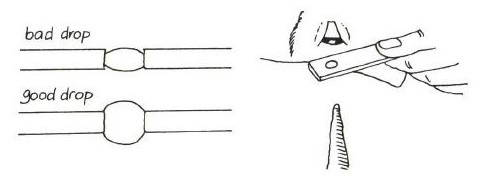
\includegraphics[width=8cm]{./img/vso/water-drop.jpg}
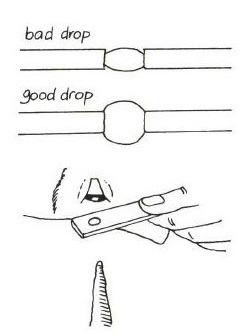
\includegraphics[width=0.45\textwidth]{./img/vso/water-drop-2.jpg}
\end{center}

\section{Slides}
A slide and even cover slip may be made from the same plastic water bottles, although being hydrophobic they will not have the same properties of glass when making wet mounts. Improvise a method for securing the punctured plastic over the slide; ideally the vertical spacing can be closely adjusted to focus.
\begin{center}
%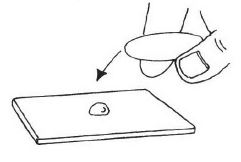
\includegraphics[width=4cm]{./img/vso/slide-cover-slip.jpg}
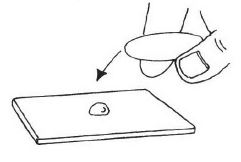
\includegraphics[width=0.45\textwidth]{./img/vso/slide-cover-slip.jpg}
\end{center}

\section{Backlighting}
On a bright day, there may not be any need for additional lighting, but in most classrooms the image will be too dim to be easily seen. The sun is a powerful light source, though not always convenient. Flashlights are generally inexpensive and available; many cell phones have one built in the end. To angle the light into the slide, find either a piece of mirror glass, wrinkle-free aluminum foil, the metalized side of a biscuit wrapper, etc.

Experiment with a variety of designs to see what works best given the materials available to your school. If you use a slide of onion cells stained with iodine solution
%(see \nameref{cha:sourcesofchemicals}, p.~\pageref{cha:sourcesofchemicals})
, your students should be able to see cell walls and nuclei.

\vfill
\columnbreak

\section{Simple Microscopes and \hfill \\ Magnifiers}

\subsection{Clear-Container Magnifiers}
\begin{center}
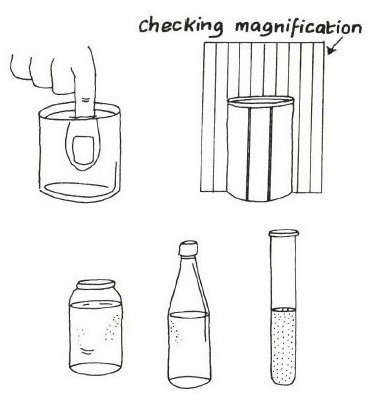
\includegraphics[width=0.4\textwidth]{./img/vso/container-microscope-2.jpg}
\end{center}

Any of these containers filled with water will make good magnifiers.

\subsection{Simple Microscope}
\begin{center}
%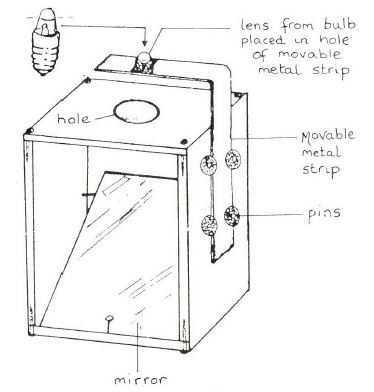
\includegraphics[width=0.49\textwidth]{./img/source/simple-microscope.jpg}
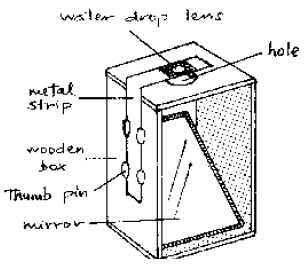
\includegraphics[width=0.49\textwidth]{./img/source/simple-microscope-2.png}
\end{center}

Construct a small wooden box from plywood as
shown (or use a small cardboard carton such as
a light bulb box). Make a round hole of 2 cm
diameter, at the top. Fit a small mirror (glass or
polished metal) in the box, angled to reflect light
up through the hole. Make a small hole (about 6
mm) in a strip of metal. Remove the round top
from a pen-torch bulb and secure it in the strip
using adhesive tape. Carefully cut off the tape
where it may cover the lens. Bend the strip, then
fix it to the side of the box, so that it can be
moved up and down. Drawing pins or nails
could be used for this. The object is focused by
moving this strip. Note the eye should be placed
as near as possible to the lens when viewing.

\vfill
\columnbreak

\subsection{Simple Compound \hfill \\ Microscope}
\begin{center}
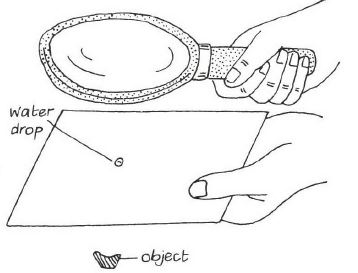
\includegraphics[width=0.4\textwidth]{./img/vso/compound-microscope.jpg}
\end{center}

\begin{itemize*}
\item Using 2 lenses together allows much greater magnification. 
\item Use a hand lens to make a water drop into a more powerful magnifier. 
\item Try using a hand lens with a lens from a torch bulb to make another simple compound microscope.
\end{itemize*}


\subsection{Card Bridge Microscope}
\begin{center}
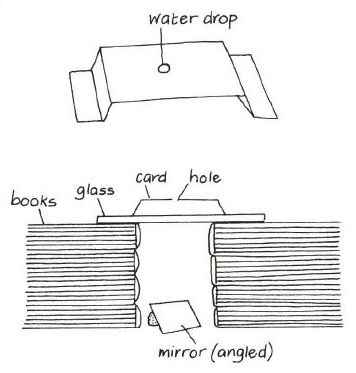
\includegraphics[width=0.4\textwidth]{./img/vso/card-microscope.jpg}
\end{center}

\begin{itemize*}
\item Place a water drop in the card `bridge'. 
\item Place this on a sheet of glass as shown. 
\item Place the object you are looking
at on the glass. This
arrangement is most suitable
for thin items, e.g. sections of leaves. 
\item Experiment with the angle of
the mirror so that light shines
up through the specimen.
\item Use this arrangement with a
hand lens to produce a
compound microscope.
\end{itemize*}

\vfill

\end{multicols}

% Part 4 - NECTA Practicals
\part{NECTA Practicals}

\chapter{Biology Practicals} \index{Practicals! Biology}

\section{Introduction to Biology Practicals} 

\subsection{Format}

%Until 2008, NECTA biology practicals contained three questions. Question 1 was required, and was a food test. Students then chose to answer either question 2 or question 3. One of these questions was usually classification.
%
%The format changed in 2008. Now, the practical contains two questions, and both are required. Food test and classification remain the most common questions, but sometimes only one of these two topics is on a given exam. The second question may cover one of a variety of topics, including respiration, transport, coordination, photosynthesis, and movement.
%
%Each question is worth 25 marks.

\subsubsection{Biology Practical Format}

The format of the Biology practical exam was revised in 2011 to keep up with the 2007 updated syllabus. As such, there will be no further Alternative to Practical exams, pending approval from the Ministry of Education.

The Biology practical has 2 questions and students must answer both. Question 1 can come from any of the following topics: Nutrition, Movement, Transport of Living Things, Respiration, Reproduction, Coordination, Regulation or Growth. Question 2 is on Classification of Living Things. Each question is worth 25 marks, and students have 2$\frac{1}{2}$ hours to complete the exam.

\subsubsection{Biology 1 Theory Format}
The theory portion of the Biology exam comprises 100 marks, while the practical carries 50 marks. A student's final grade for Biology is thus found by taking her total marks from both exams out of 150.

The theory exam for Biology contains 13 questions over 3 sections. Section A has 2 questions worth 10 marks each.  Section B has 8 short answer questions, each having two items. This section weighs a total of 60 marks, and the mark allocation for individual questions is indicated at the end of each question. Section C has 3 long answer\slash essay questions, though students only need to answer 1 of them. The answer must be comprehensive and include as many points as possible. It is worth 20 marks.

\paragraph{Note} This information is current as of the time of publication of this manual. Updated information may be obtained by contacting the Ministry of Education. 

\subsection{Notes for Teachers}

\subsubsection{NECTA Advance Instructions}
Advance instructions are given to teachers at least one month before the date of the exam, as well as 24 hour advance instructions, to enable them to prepare apparatus, equipment and materials required for the examination.

%[tips for identifying practicals from advance instructions, example advance instructions?]

%\subsubsection{Words of Advice}

%\subsection{NECTA Marking Information}
%[how NECTA marks the practicals, highlight most important parts]

\subsection{Common Practicals}
\begin{description}
\item[Food Tests]{test a food solution for starch, sugars, fats, and protein}
\item[Classification]{name and classify specimens, then answer questions about their characteristics}
\item[Respiration]{use lime water to test air from the lungs for carbon dioxide}
\item[Transport]{investigate osmosis by placing leaf petioles or pieces of raw potato in solutions of different solute concentrations}
\item[Photosynthesis]{test a variegated leaf for starch to prove that chlorophyll is necessary for photosynthesis}
\item[Coordination]{students look at themselves in the mirror and answer questions about the sense organs they see}
\item[Movement]{name bones and answer questions about their structure and position in the body}
\end{description}

\paragraph{Note} These are the most common practicals, but they are not necessarily the only practicals that can occur on the national exam. Food tests and Classification are by far the most common, but there are many eligible topics. Be sure to regularly look through \nameref{cha:past-papers-bio} (p.~\pageref{cha:past-papers-bio}) to get an idea of the kind of questions that can occur.

%==============================================================================
\section{Food Tests} \index{Practicals! Biology! food tests} \index{Food tests}

In this practical, students test a solution of unknown food substances for starch, protein, reducing sugars, non-reducing sugars, and lipids. They record their procedure, observation, and conclusions, then answer questions about nutrition and the digestive system.\\

\noindent This section contains the following:
\begin{itemize}
\item{Preparation of Chemical Solutions}
\item{Preparation of Food Solutions}
\item{Performing the Food Tests}
\item{Examination Room}
\item{Student Report}
\item{Sample Food Test Practical}
%\item{Sample Food Test Solutions}
\end{itemize}

\subsection{Preparation of Chemical Solutions}
Always make sure the chemicals work before performing the food tests with students.

\subsubsection{Benedict's Solution} \index{Benedict's solution! for food tests}
This solution can be bought at a chemical store already prepared or you can make it yourself.\\

\textbf{Using Sodium Carbonate:}
\begin{itemize*}
\item Add about 1 L of water to a plastic bottle.
\item Add 5 spoons of sodium carbonate (NaCO$_3$).
\item Add 3 spoons of citric acid.
\item Add one spoon of copper sulphate.
\end{itemize*}

\textbf{Using Bicarbonate of Soda:}
\begin{itemize*}
\item Add 1 L of water to a cooking pot.
\item Add a box (70 g) of bicarbonate of soda.
\item Boil the mixture for 5-10 minutes. This makes sodium carbonate.
\item Let cool and transfer to a plastic water bottle.
\item Add 3 spoons of citric acid.
\item Add one spoon of copper sulphate. Cap and shake to mix.
\end{itemize*}

\noindent Label as: BENEDICT'S SOLUTION FOR FOOD TESTS

\noindent The solution may be stored in any plastic or glass bottle and will keep indefinitely.

\subsubsection{Copper (II) Sulphate} \index{Copper sulphate! for food tests}
\begin{itemize*}
\item Add one spoon of copper (II) sulphate to a 1.5 L bottle.
\item Add 1 L of water and shake until chemicals are fully dissolved.
\end{itemize*}

\noindent Label as: 1\% COPPER (II) SULPHATE SOLUTION FOR FOOD TESTS

\noindent The solution may be stored in any plastic or glass bottle and will keep indefinitely.

\subsubsection{Iodine Solution} \index{Iodine solution! for food tests}
Make sure to use iodine tincture from a pharmacy. The tincture must not contain ethanol\slash alcohol\slash spirit.

\begin{itemize*}
\item Add 1 part iodine tincture to 10 parts water. Example: In a 500 mL bottle, add 40 mL iodine tincture, then and 400 mL of water.
\item Cap the bottle and shake.
\end{itemize*}

\noindent Label as: IODINE SOLUTION FOR FOOD TESTS

\noindent The solution may be stored in any plastic or glass bottle and will keep indefinitely.

\subsubsection{Dilute NaOH} \index{Sodium hydroxide! for food tests}
\begin{itemize*}
\item Using a PLASTIC teaspoon, add one level teaspoon of NaOH to a 500 mL water bottle. Caustic soda (NaOH) reacts with metal. DO NOT TOUCH.

\emph{SAFETY NOTE: Prepare about 100 mL of citric acid or ethanoic acid solution to neutralize sodium hydroxide spills on skin or lab tables. One spoon of citric acid in 100 mL of water is suitable. Ethanoic acid solutions are sold in stores as vinegar.}

\item Add 250 mL of water.

\emph{SAFETY NOTE: This reaction can cause the solution to become very warm. Avoid chemical burns by wearing gloves.}

\item Cap well and shake. This makes 1 M sodium hydroxide solution.
\end{itemize*}

\noindent Label as: 1 M SODIUM HYDROXIDE SOLUTION FOR FOOD TESTS (CORROSIVE)

\noindent The solution will react with carbon dioxide in the air if not well sealed. Do not store in glass bottles with glass stoppers as these will stick. The solution may be stored in plastic bottles indefinitely.


\subsubsection{Dilute Acid} \index{Hydrochloric acid! for food tests} \index{Citric acid! for food tests}
Your school may have dilute hydrochloric acid or you may have to make it yourself.\\

\textbf{Using Hydrochloric Acid (HCl):}
\begin{itemize*}
\item Add 1 part HCl to 9 parts water. Example: In a 1.5 L water bottle, add 900 mL of water, then add 100 mL of HCl.
\item Shake well.
\end{itemize*}

\textbf{Using Citric Acid:}
\begin{itemize*}
\item Add 500 mL of water to a 1 or 1.5 L water bottle.
\item Add 5 spoons of citric acid.
\item Cap well and shake. This makes 0.5 M citric acid.
\end{itemize*}

\noindent Label as: 0.5 M CITRIC ACID FOR FOOD TESTS

\noindent The solution may be stored in any plastic or glass bottle and will keep indefinitely.

\subsubsection{Sudan III Solution} \index{Sudan III solution! for food tests}
Using Sudan III solution takes a long time to show results. It may be replaced by iodine tincture solution for the lipids test.

\begin{itemize*}
\item Combine 0.5 g of Sudan III powder with 100 mL of 70\% ethanol solution (30 mL water and 70 mL ethanol).
\item Place the solution in a warm water bath to help the Sudan III dissolve.
\item Filter to remove any remaining solid.
\end{itemize*}

\noindent Label as: SUDAN III SOLUTION FOR FOOD TESTS

\noindent The solution may be stored in any plastic or glass bottle and will keep indefinitely.


\subsection{Preparation of Food Solutions}
For the NECTA and mock exams you may have to set up the food test solutions. The instructions will tell you which ones you'll need to prepare in order to make `Solution X.' Solution X consists of a mixture of at least 3 of the different food substances and is given to each student in at least 3 test tubes. Make sure food solutions are well-dissolved and colorless so that students don't know what is in the mixture. You don't need to measure the ingredients, but make sure to test the solutions before the practical.

\subsubsection{Reducing sugar}
Use glucose powder and dissolve in water. Make sure the substance is fully dissolved so that students don't know what is in the mixture.

\subsubsection{Non-reducing sugar}
Use sugar and dissolve in water. Make sure the substance is fully dissolved so that students don't know what is in the mixture.

\subsubsection{Lipids}
Mix sunflower oil with water. Shake immediately before use. Sunflower oil is best since it is liquid at room temperature.

\subsubsection{Protein}
Mix an egg white with water.

\subsubsection{Starch}
Save the water you use to boil potatoes, rice, or pasta. Make sure to remove the bits of food. You can also just mix flour in water, but it would be obvious.


\subsection{Performing the Food Tests}

\subsubsection{Reducing Sugars Test}
\begin{itemize*}
\item Add a small amount of Benedict's solution to the food solution. 
\item Boil the solution and allow it to cool. Observe the colour changes from blue to green, yellow, then deep orange\slash brick red precipitate if reducing sugars are present.
\end{itemize*}
Always do the reducing sugars test first because a non-reducing sugar will always test positive for a reducing sugar.

\subsubsection{Non-reducing Sugars Test}
\begin{itemize*}
\item Add a small amount of dilute acid (HCl) to the solution. 
\item Boil the solution for about 30 seconds and allow it to cool. 
\item Add a small amount of NaOH to the solution and shake.
\item Add a small amount of Benedict's solution and boil. 
\item Allow the solution to cool and observe as the solution changes from green to yellow, then to deep orange\slash brick red precipitate if non-reducing sugars are present.
\end{itemize*}

\subsubsection{Lipids Test}
\begin{itemize*}
\item Add a small amount of Sudan III or iodine solution to the food solution and shake. 
\item A red ring will form at the top of the test tube if lipids are present.
\end{itemize*}
Using Sudan III colours the whole solution red whether it contains lipids or not. Use iodine solution to get a more distinct result.

\subsubsection{Protein Test}
\begin{itemize*}
\item Add an \emph{equal} amount of sodium hydroxide (NaOH) to the solution and shake. 
\item Add a small amount of copper (II) sulphate to the solution and shake.
\item Observe the solution turn violet\slash purple in colour if protein is present.
\end{itemize*}

\subsubsection{Starch Test}
\begin{itemize*}
\item Add a small amount of iodine solution to the food solution.
\item Observe the solution turn blue-black in colour if starch is present.
\end{itemize*}


\subsection{Examination Room}
The NECTA practical exam is done in the school's lab or any other suitable room. Heat sources (jiko, etc.) should be spread evenly in the exam room so that students don't have to go far to heat their test tubes; this also cuts down on cheating. Spread students out and distribute supplies as you see fit.\\

\noindent \textbf{Each student gets:}
\begin{itemize*}
\item[-] 3 or more test tubes (to carry out 5 tests)
\item[-] A beaker containing Solution X
\item[-] A test tube rack (or a cut out water bottle with sand to hold the tubes)*
\end{itemize*}
* Students may share the racks, but shouldn't share the cut out bottles\\

\noindent \textbf{Each station should have:}
\begin{itemize*}
\item[-] Copper II sulphate
\item[-] Water
\item[-] Dilute acid (HCl, etc.)
\item[-] Dilute base (sodium hydroxide)
\item[-] Iodine solution
\item[-] Sudan III solution (can be replaced by iodine solution)
\item[-] Benedict's solution
\end{itemize*}

\subsection{Student Report}
Food test data is recorded in a table containing four columns: Test for, Procedure, Observation and Inference.

Students should write the Procedure using the passive voice in the past tense. For example, ``A small amount of Benedict's solution was added to the solution. Then the solution was boiled and allowed to cool.''

In the Observation column, the student should write what they observed using the past tense and passive voice. For example, ``A violet colour was observed.''

In the Inferences column, the students should write what they saw in the past tense and passive voice. For example, ``Reducing sugars were not (or were) present.''

Note that every column is worth marks on the exam. Even if students fail to do the food tests correctly, they can still get marks for writing what they are testing for and what the procedure should be.

An example of a completed food test results table is given below. Assume the solution contains proteins, reducing sugars, non-reducing sugars and starch.

\begin{center}
\begin{tabular}{|p{3cm}|p{5cm}|p{3cm}|p{3cm}|} \hline
\multicolumn{1}{|c|}{\textbf{Food Tested}}&\multicolumn{1}{c|}{\textbf{Procedure}}&\multicolumn{1}{c|}{\textbf{Observation}}&\multicolumn{1}{c|}{\textbf{Inference}} \\ \hline
Lipids & A few drops of Sudan III solution (or iodine solution) were added to solution X. The solution was shaken and allowed to stand. & A red ring did not form at the surface. & Lipids were not present.\\ \hline
Proteins & An equal amount of NaOH was added to solution X and shaken. A few drops of copper (II) sulphate were added to solution X and shaken again. & A violet colour was observed. & Proteins were present.\\ \hline
Reducing sugars & A small amount of Benedict's solution  was added to solution X. The solution was heated and allowed to cool. & A brick red precipitate was observed. & Reducing sugars were present.\\ \hline
Non-reducing sugars & A small amount of dilute acid was added to solution X. The solution was heated and allowed to cool. Then a small amount of NaOH solution was added, and the solution was shaken. Finally, a small amount of Benedict’s solution was added. The solution was boiled and let cool. & The solution changed from green to yellow, then to a deep orange\slash brick red precipitate. & Non-reducing sugars were present.\\ \hline
Starch & A few drops of iodine solution were added to solution X and shaken. & A blue-black colour was observed. & Starch was present.\\ \hline
\end{tabular}
\end{center}

\subsection{Sample Food Test Practical}
You have been provided with solution \textbf{B}. 

\begin{enumerate}
\item[(a)] Identify the food substances present in solution \textbf{B} by using the reagents provided. Tabulate your work as shown in the following Table:

\begin{center}
\begin{tabular}{|p{3cm}|p{3cm}|p{3cm}|p{3cm}|} \hline
\multicolumn{1}{|c|}{\textbf{Food Tested}}&\multicolumn{1}{c|}{\textbf{Procedure}}&\multicolumn{1}{c|}{\textbf{Observation}}&\multicolumn{1}{c|}{\textbf{Inference}} \\ \hline
&&& \\
&&& \\
&&& \\
&&& \\ \hline
\end{tabular} \\[10pt]
\end{center}

\item[(b)] For each food substance identified in 1(a);
\begin{enumerate}
\item[(i)] Name two common sources.
\item[(ii)] State their role in the body of human being.
\end{enumerate}
\item[(c)] The digestion of one of the identified food substance in 1(a) starts in the mouth.
\begin{enumerate}
\item[(i)] Name this food substance.
\item[(ii)] Identify the enzyme responsible for its digestion in the mouth.
\end{enumerate}
\item[(d)] The digestive system of human being has several parts.
\begin{enumerate}
\item[(i)] Name the part of digestive system in which most of digestion and absorption of food takes place.
\item[(ii)] Explain how the named part in (d) (i) is adapted for absorption of digested food substances.
\end{enumerate}
\end{enumerate}

\textbf{Additional Food Test Questions:}
See \nameref{cha:past-papers-bio} (p.~\pageref{cha:past-papers-bio}) for additional food test questions.

%\begin{enumerate*}
%\item[(e)] What is the function of each of the food substances in solution \textbf{B} to human beings? 
%\item[(f)] For each food substance identified, name the enzyme and end product of digestion 
%taking place in the:\\
%\begin{enumerate*}
%\item[(i)] Stomach
%\item[(ii)] Duodenum
%\end{enumerate*}
%\item[(g)] What deficiency diseases are caused by a lack of the identified food substances?
%\end{enumerate*}


%\subsection{Sample Food Test Solutions}



%\section{Food Tests}
%
%In this practical, students test a solution of unknown food substances for starch, protein, reducing sugars, non-reducing sugars, and fats\slash oils. They record their procedure, observation, and conclusions, then answer questions about nutrition and the digestive system.
%
%This section contains the following:
%\begin{itemize}
%\item{Preparation of test solutions}
%\item{Preparation of food solutions}
%\item{How to carry out food tests}
%\item{How to write a report}
%\item{Sample practical with solutions}
%\end{itemize}
%
%\subsection{Test for Starch}
%
%\subsubsection{Materials}
%\begin{itemize}
%\item{iodine tincture from the pharmacy (any brand)}
%\item{tap or clean river water}
%\end{itemize}
%
%\subsubsection{Procedure to make 400~mL}
%\begin{enumerate}
%\item{40~mL of iodine tincture to a 500~mL plastic water bottle.}
%\item{Add about 400~mL of water.}
%\item{Cap the bottle and shake.}
%\item{Use a permanent pen to label the bottle:\\
%IODINE SOLUTION FOR FOOD TESTS}
%
%The solution may be stored in any plastic or glass bottle and will keep indefinitely.
%\end{enumerate}
%
%\subsection{Test for protein}
%
%The best test for protein is the Biuret test. This requires two solutions: 1\% \ce{CuSO4} and 1~M \ce{NaOH}.
%
%\subsubsection{Materials}
%\begin{itemize}
%\item{copper sulfate}
%\item{sodium hydroxide}
%\item{tap or clean river water}
%\end{itemize}
%
%\subsubsection{Procedure to make 1~L copper sulfate solution}
%\begin{enumerate}
%\item{Use a small metal or plastic spoon (tea size) to transfer one level spoon of copper sulfate into a 1 or 1.5~L water bottle.}
%\item{Add about one liter of water. The amount does not have to be exact.}
%\item{Cap the bottle and shake until the copper sulfate has completely dissolved.}
%\item{Use a permanent pen to label the bottle:\\
%1\% Copper (II) Sulfate Solution\\
%For food tests}
%\end{enumerate}
%
%The solution may be stored in any plastic or glass bottle and will keep indefinitely.
%
%\subsubsection{Procedure to make 250~mL of sodium hydroxide solution}
%\begin{enumerate}
%\item{Use a small PLASTIC spoon (tea size) to transfer one level spoon of sodium hydroxide into a 500~mL water bottle. Caustic soda (sodium hydroxide) reacts with metal. DO NOT TOUCH.
%
%\textit{SAFETY NOTE: prepare about 100~mL of citric acid or ethanoic acid solution to have available to neutralize sodium hydroxide spills on skin or lab tables. One spoon of citric acid in about 100~mL of water is a suitable concentration. Ethanoic acid solutions of the proper concentration are sold in food shops as vinegar.}
%
%}%item
%
%\item{Add about 250~mL of water to the bottle. In the new 500~mL Maji Africa bottles, this is the first straight line above the curving lines. The addition of water to sodium hydroxide gets HOT.}
%\item{Cap the bottle very well and shake to mix.}
%\item{Use a permanent pen to label the bottle:\\
%1~M SODIUM HYDROXIDE SOLUTION FOR FOOD TESTS\\
%CORROSIVE. Neutralize spills with weak acid solution.}
%\end{enumerate}
%
%The hydroxide solution will react with carbon dioxide in the air if the container is not well sealed. The solution should not be stored in glass bottles with glass stoppers for overnight or longer as these will stick. The solution may be stored in plastic bottles indefinitely.
%
%\subsection{Test for lipids}
%
%\subsubsection{Materials}
%\begin{itemize}
%\item{Provodine iodine tincture from the pharmacy -- the tincture must be without ethanol\slash alcohol\slash ``spiriti''}
%\item{tap or clean river water}
%\end{itemize}
%
%\subsubsection{Procedure to make 400~mL}
%See instructions for preparing iodine solution for Test for Starch above.
%
%\subsubsection{A note on theory}
%
%Many biology books call for a chemical called Sudan III to test for lipids. Sudan III is a bright red pigment that is much more soluble in oil than in water. For this reason, Sudan III solution is usually prepared using ethanol to bring the Sudan III pigment into the solution. In mixtures of oil and water, the oil separates and moves to the top. When shaken with Sudan III, this oil absorbs the Sudan III, turns red, and produces a ``red ring'' at the top of the test tube. However, the ethanol used to make Sudan III causes the water and oil to form an emulsion. In an emulsion, the oil is broken into very small particles and it takes a long time for this emulsion to break down and form an oil layer on the top. Hence testing with Sudan III takes a long time to show a clear result.
%
%Iodine is another coloured molecule that is more soluble in oil than in water. When a mixture of oil and water is shaken with iodine solution, the iodine moves to the oil layer, colouring it orange or red. This also gives the result of a ``red ring'' at the top of the test tube. To prevent an emulsion forming -- as happens with Sudan III -- it is very important to make iodine solution from pharmacy tincture that is without ethanol. Another benefit of using iodine is that while Sudan III is always red, iodine is uniquely yellow in water and red in oil, making the difference between positive and negative results easier to see. Because there is no ethanol in iodine solution, the result also comes much faster, usually within 10-20 seconds.
%
%Note that if the oil and water mixture settles before you transfer it to the test tube, there may be too little or too much oil in the test tube. Shake the food sample solution before taking each sample.
%
%\subsection{Test for reducing sugars with Benedict's solution}
%
%\subsubsection{Materials}
%\begin{itemize}
%\item{sodium carbonate (soda ash) if available, otherwise sodium hydrogen carbonate (bicarbonate of soda)}
%\item{citric acid}
%\item{copper sulfate}
%\item{tap or clean river water}
%\item{plastic water bottle with screw cap}
%\end{itemize}
%
%\subsubsection{Procedure to make 1~L using soda ash}
%Combine the following into the bottle in order, adding slowly:
%\begin{enumerate}
%\item{about 1~L water}
%\item{five spoons of sodium carbonate}
%\item{three spoons of citric acid}
%\item{one spoon of copper sulfate.}
%\end{enumerate}
%
%All measurements with the spoon should be level to ensure that the volume measured is consistent. The final solution should have a bright blue color.
%
%\subsubsection{Procedure to make 500~mL using sodium hydrogen carbonate}
%\begin{enumerate}
%\item{Add 500~mL of water to a cooking pot.}
%\item{Add a box (70~g) of bicarbonate of soda to the water.}
%\item{Heat the pot on a stove until boiling. Let boil for ten minutes.}
%\item{Remove the pot from the stove and let cool. When cool, transfer the liquid to a plastic water bottle.}
%\item{Slowly add one and a half spoons of citric acid.}
%\item{Add half a spoon of copper sulfate. Cap and shake to mix.}
%\end{enumerate}
%
%Label the final solution:
%
%\begin{center}	
%BENEDICT'S SOLUTION FOR FOOD TESTS.
%\end{center}
%
%The solution may be stored in any plastic or glass bottle and will keep indefinitely.
%
%\subsection{Test for non-reducing sugar}
%
%\subsubsection{Materials}
%\begin{itemize}
%\item{Benedict's solution, above}
%\item{1M sodium hydroxide solution, above under protein test}
%\item{citric acid}
%\item{tap or clean river water}
%
%To perform this test, students first test their sample with Benedict's solution to eliminate the possibility of a reducing sugar. Then, they must use an acid solution to hydrolyze any non-reducing sugars and then a base solution to neutralize the sample solution. Then the students perform again the test for non-reducing sugars.
%
%\subsubsection{Procedure to make 500~mL of acid solution}
%\begin{enumerate}
%\item{Put 500~mL of water into a plastic water bottle.}
%\item{Add five spoons of citric acid.}
%\item{Cap the bottle very well and shake to mix.}
%\item{Use a permanent pen to label the bottle:\\
%0.5~M CITRIC ACID FOR FOOD TESTS}
%\end{enumerate}
%
%The solution may be stored indefinitely in any plastic or glass container.
%
%\subsection{Preparation of Food Sample Solutions}
%
%Try to make food solutions colorless so that students cannot guess what is in them, and so that they can see the colors that form during food tests. You do not need to measure the ingredients of the solution, but make sure to test solutions before the practical.
%
%\subsubsection{Starch solution}
%The easiest solution is the water left from boiling pasta or potatoes. If you have been only ugali and rice lately, add some wheat or corn flour to boiling water. Let cool. Decant the solution or filter it with a tea filter to remove the largest particles. If you are in a hurry, you can also just mix flour with cold water, but then it will be obvious that flour is present.
%
%\subsubsection{Lipids}
%Add cooking oil to water. Shake immediately before use. Sunflour oil is best – avoid fats that solidify near room temperature.
%
%\subsubsection{Protein solution}
%Combine egg whites with water. If you do not have egg whites, you can use fresh or powder milk, although this will give the solution a white color and add a reducing sugar (lactose). The water used in boiling beans also contains some protein, but it may not be enough to see a color change.
%
%\subsubsection{Reducing sugar}
%The easiest is to buy glucose powder from a shop and dissolve it in water. You can also grind pieces of onion with water and filter the resulting solution.
%
%\subsubsection{Non-reducing sugar}
%Dissolve sugar in water. Table sugar is sucrose, a non-reducing sugar.
%
%\subsection{How to Carry Out Food Tests}
%
%\subsubsection{Starch}
%Add a few drops of iodine to the solution and shake well. A blue-black color forms if starch is present
%
%\subsubsection{Lipids}
%Add a few drops of iodine to the solution and shake well. A red ring will form at the top of the test tube is lipids are present.
%
%You can also have your students do the grease spot test -- rub a drop of solution onto a piece of paper, and let dry. A translucent spot forms if fat is present. This test is great for its simplicity, but is not used on national exams.
%
%\subsubsection{Protein (Biuret test)}
%Add a few drops of 1~M \ce{NaOH} to the solution and shake well. Then add a few drops of 1\% \ce{CuSO4} solution and shake. A violet color forms if protein is present. Sometimes the color takes a minute or two to appear. 
%
%Some textbooks may recommend using Millon's reagent to test for protein. This reagent contains mercury, which is extremely poisonous and should never be handled by students.
%
%The purple colour from a positive test is the result of a complex between four nitrogen atoms and the copper (II) ion. Specifically, these nitrogen atoms are all part of peptide bonds. These peptide bonds are adjacent on a protein, either two from one protein and two from another, or two from one part of a protein and two from another part of the same protein.
%
%\subsubsection{Reducing sugar}
%Place some food solution in a test tube, and add an equal volume of Benedict’s solution. Heat to boiling, then let cool. A brick red or orange precipitate forms if a reducing sugar is present.
%
%Benedict's solution contains aqueous copper (II) sulphate, sodium carbonate, and sodium citrate. The citrate ions in Benedict's solution complex the copper (II) ions to prevent the formation of insoluble copper (II) carbonate. In the presence of a reducing sugar, however, the copper (II) ions are reduced to copper (I) ions which form a brick red precipitate of copper (I) oxide. The oxygen in the copper (I) oxide come from hydroxide; the purpose of the sodium carbonate is to provide this hydroxide by creating an alkaline environment.
%
%Normally, sugar molecules form five or six member rings and have no reducing properties. In water, however, the rings of some sugar molecules can open to form a linear structure, often with an aldehyde group at one end. These aldehyde groups react with copper (II) to reduce it to copper (I). Sugars that do not have an aldehyde group in the linear structure or that are not able to open are not able to reduce copper (II) ions and are thus called non-reducing sugars. Students do not need to understand this chemistry for their exam, but they may ask about what is happening in the reaction.
%
%\subsubsection{Non-reducing sugar}
%Do the test for a reducing sugar using Benedict's solution. Notice that no reaction occurs. Add a few drops of citric acid solution to the solution, then heat to boiling. Let solution cool. Add a few drops of 1~M \ce{NaOH}, and shake well. Then, add some Benedict’s solution (equal in volume to the liquid in the test tube). Boil the solution, and let it cool. A brick red or orange precipitate forms if a non-reducing sugar is present.
%
%This experiment will also test positive for all reducing sugars. Therefore it is important to first perform the test for reducing sugars before considering this test. If the test for reducing sugars is positive, there is no reason to perform the test for non-reducing sugars -- the conclusion will be invalid.
%
%Non-reducing sugars are a misnomer, that is, their name is incorrect. This test does not test for any sugar that is not reducing. Rather, this is a test for any molecule made of multiple reducing sugars bound together, such as sucrose or starch. When these polysaccharides are heated in the presence of acid, they hydrolyse and release monosaccharides. The presence of these monosaccharides is then identified with Benedict's solution.
%
%The purpose of the sodium hydroxide is to neutralize the citric acid added for hydrolysis. If the citric acid is not hydrolysed, it will react with the sodium carbonate in Benedict's solution, possibly making the solution ineffective.
%
%\subsection{How to Write a Report}
%Food test data is reported in a table containing four columns: test for, procedure, observation, and inference. With the exception of the `test for' column, data should be reported in full sentences written in past tense. The procedure should also be in passive voice. No, this is not the way professional scientists write. However, students here must use passive voice to get marks on the national exam.
%
%Note that every column is worth marks on the exam. Even if students fail to do the food tests correctly, they can still get marks for writing what they are testing for and what the procedure should be.
%
%See the sample practical below for an example of a report.
%
%\subsection{Sample Food Test Practical}
%
%You have been provided with Solution K. Carry out food test experiments to identify the food substances present in the solution.
%\begin{enumerate}
%
%\item{Record your experimental work as shown in the table below.}
%
%\begin{center}
%\begin{tabular}{| c | c | c | c |}
%\hline
%Test for & Procedure & Observations & Inferences\\ \hline
%Protein & & & \\ \hline
%Starch & & & \\ \hline
%Lipids & & & \\ \hline
%Reducing sugars & & & \\ \hline
%Non-reducing sugars & & & \\ \hline
%\hline
%\end{tabular}
%\end{center}
%
%\item{Suggest two natural food substances from which solution K might have been prepared.}
%\item{What is the function of each of the food substances in solution K to human beings?}
%\item{For each food substance identified, name the enzyme and end product of digestion taking place in the:}
%\begin{enumerate}
%\item{Stomach}
%\item{Duodenum}
%\end{enumerate}
%\item{What deficiency diseases are caused by a lack of the identified food substances?}
%\end{enumerate}
%
%\subsection{Sample Practical Solutions}
%(Assume Solution K contains protein and starch.)
%
%\item{The results were as follows}
%
%\begin{center}
%\begin{tabular}{| c | c | c | c |}
%\hline
%Test for & Procedure & Observations & Inferences\\ \hline
%Protein & 
%A few drops of NaOH solution & A violet color & Protein was present. \\
%& were added to Solution K. & was observed. &\\
%& The solution was shaken.& & \\
%& Then a few drops of & &\\
%& \ce{CuSO4} solution were & & \\
%& added to Solution K, and the & &\\
%& solution was shaken again. & &\\ \hline
%Starch & A few drops of iodine & A blue-black color & Starch was present. \\
%& solution were added & was observed. & \\
%& to Solution K, and & & \\
%& the solution was shaken. & & \\ \hline
%Lipids & A few drops of Sudan III & A red ring did not & Fats/oils were absent. \\
%& solution (or iodine solution) & form at the surface. & \\
%& were added to Solution K. & & \\
%& The solution was shaken & & \\ 
%& and then allowed to stand. & & \\ \hline
%Reducing & A small amount of Benedict’s & There was no & Reducing sugars  \\
%sugars & solution was added & precipitate & were absent.\\
%& to Solution K. & & \\
%& The solution was boiled & & \\
%& and allowed to cool. & & \\ \hline
%Non- & A small amount of dilute & There was no & Non-reducing \\
%reducing & acid was added to & precipitate.& sugars were absent.\\
%sugars & Solution K. The solution & &\\
%& was boiled and allowed to cool. & & \\
%& Then a small amount of & & \\
%& NaOH solution was added, & & \\
%& and the solution was shaken. & & \\
%& Finally, a small amount of & & \\
%& Benedict’s solution was added. & & \\
%& The solution was boiled & & \\
%& and let cool. & &\\ \hline
%\hline
%\end{tabular}
%\end{center}
%
%\item{Solution K could have been prepared from egg and maize. \textit{(Note: Any non-processed food containing protein or starch is correct here.)}}
%\item{Starch provides energy to the body. Proteins are used in growth and tissue repair.}
%
%\begin{center}
%\begin{tabular}{| c | c | c | c |}
%\hline
%Food Substance & Location & Enzyme & End Product of Digestion\\ \hline
%Protein & Stomach & \textit{Pepsin} & Polypeptides \\ \hline
%Protein & Duodenum & \textit{Trypsin} & Amino acids \\ \hline
%Starch & Duodenum & \textit{Pancreatic amylase} & Maltose \\ \hline
%\hline
%\end{tabular}
%\end{center}
%
%\item{A deficiency of protein causes kwashiorkor. A deficiency of starch causes marasmus.}
%\end{itemize}

%==============================================================================
\section{Classification} \index{Practicals! Biology! classification} \index{Classification}

The classification practical requires students to identify specimens of animals, plants, and fungi. The students must write the common name, kingdom, phylum, and sometimes class of each specimen. They also answer questions about the characteristics and uses of the specimens.

This section contains the following:
\begin{itemize}
\item{Common specimens}
\item{Where to find specimens}
\item{Storage of specimens}
\item{Sample practical with solutions}
\item{Additional classification questions}
\end{itemize}

\subsection{Common Specimens}
\begin{description}
\item[Fungi]{Mushroom, yeast, bread mold}
\item[Plants]{Fern, moss, bean plant, bean seed, maize plant, maize seed, pine tree, cactus, sugar cane, Irish potato1, cypress tree, acacia tree, hibiscus leaf, cassava}
\item[Animals]{Millipede, centipede, grasshopper, lizard, tilapia (fish)3, scorpion, frog, tapeworm, liver fluke, cockroach, spider}
\end{description}

\subsection{Where to Find Specimens}
\begin{itemize}
\item{Start collecting specimens several months before the NECTA exams, as some specimens can be hard to find in the dry season.}
\item{Ask your students to bring specimens! Students are especially good at finding insects and other animals. You can even find primary school children to gather insects such as grasshopper and millipedes.}
\item{Ferns, hibiscus, pines, and cypresses are used in landscaping. Try looking near nice hotelis or guestis. Ferns should have sori (sporangia) on the underside of their leaves.}
\item{Moss often grows near water tanks and in shady corners of courtyards. It is hard to find in the dry season.}
\item{Sugarcane, Irish potato, cassava, tilapia, bean seeds, and maize seeds can be found at the market. Yeast is available at shops.}
\item{Mushrooms are hard to find in the dry season. However, they are available at grocery stores in large cities, and you may be able to find dried mushrooms at the market. You can also collect mushrooms in the rainy season and dry them yourself.}
\item{Tapeworms and liver flukes may be acquired from butchers. Find out where livestock is slaughtered and ask the butchers to look for worms (minyoo). Liver flukes are found in the bile ducts inside the liver, while tapeworms are found in the intestines. You can also try going to a livestock fair\slash market (mnada) or talking to the local meat inspector (mkaguzi wa nyama).}
\item{Grow your own bread mold. Just put some bread in a plastic bag and leave it in a warm place. But do it ahead of time -- it can take two weeks to obtain bread mold with visible sporangia.}
\end{itemize}

\subsection{Storage of Specimens}
\begin{itemize}
\item{Insects and mushrooms can be dried and stored in jars. However, they become brittle and break easily.}
\item{A 10\% solution of formaldehyde is the best way of storing specimens. Formaldehyde is often sold as a 40\% solution. It should be stored in glass jars and out of the sun. Check specimens periodically for evaporation. Formaldehyde works because it is toxic; handle carefully.}
\item{In a pinch, a 70\% solution of ethanol can also be used to store insects, lizards, and worms. However, specimens sometimes decay in ethanol.}
­­\end{itemize}

\subsection{Sample Classification Practical}

You have been provided with specimens L, M, N, O, and P.
\begin{enumerate}
\item{Identify the specimens by their common names.}
\item{Classify each specimen to the phylum level.}	
\item{Further classification:}
\begin{enumerate}
\item{Write the classes of specimens L and M.}
\item{List two observable differences between specimens L and M.}
\end{enumerate}
\item{Explain why specimen P cannot grow taller.}
\item{Write down two distinctive characteristics of the phylum to which specimen O belongs.}
\item{Reproduction:}
\begin{enumerate}
\item{List the modes of reproduction in specimens M and N.}
\item{What are two differences between these modes of reproduction?}
\end{enumerate}
\end{enumerate}

\subsection{Sample Practical Solutions}

\begin{enumerate}

\item{Common names of specimens:}
\begin{itemize}
\item{L: maize plant}
\item{M: bean plant}
\item{N: yeast}
\item{O: millipede}
\item{P: moss}
\end{itemize}


\item{Classifaction by kingdom and phylum:}

\begin{center}
\begin{tabular}{| c | c | c |}
\hline
Specimen & Kingdom & Phylym \\ \hline
L (maize plant) & Plantae & Angiospermophyta \\ \hline
M (bean plant) & Plantae & Angiospermophyta \\ \hline
N (yeast) & Fungi & Ascomycota \\ \hline
O (millipede) & Animalia & Arthropoda \\ \hline
P (moss) & Plantae & Bryophyta \\ \hline
\hline
\end{tabular}
\end{center}

\item{Further classification:}
\begin{itemize}
\item{Specimen L (maize plant): Class Monocotyledonae}
\item{Specimen M (bean plant): Class Dicotyledonae}
\item{Observable differences:}

\begin{center}
\begin{tabular}{| c | c | c |}
\hline
Specimen & Vein structure & Root structure \\ \hline
L (maize plant) & Parallel veins & Fibrous roots \\ \hline
M (bean plant) & Net veins & Tap roots \\ \hline
\hline
\end{tabular}
\end{center}

\textit{The answers to this question should be differences between monocots and dicots that the student can see by observing the plants with their naked eyes. Hence answers such as ``vascular bundles in a ring'' are not correct.}

\end{itemize}

\item{Specimen P (moss) cannot grow taller because it has no xylem and phloem. If it grew taller, it would not be able to transport food and water throughout the plant.}
\item{Characteristics of phylum Arthropoda:}
\begin{itemize}
\item{jointed legs}
\item{segmented body}
\item{exoskeleton made of chitin}
\end{itemize}
\item{Reproduction}
\begin{enumerate}
\item{Specimen M (bean plant) reproduces by sexual reproduction. Specimen N (yeast) reproduces by asexual reproduction.}

\begin{center}
\begin{tabular}{| c | c | c | c |}
\hline
Method & Genetic variation & Parents & Gametes \\ \hline
Asexual & There is no genetic & Requires one & No gametes  \\
reproduction & variation between offspring. & parent only. & are involved. \\ \hline
Sexual & There is genetic & Usually requires & Involves fusion  \\
reproduction & variation between offspring. & two parents. & of two gametes.\\ \hline
\hline
\end{tabular}
\end{center}

\end{enumerate}
\end{enumerate}

\subsection{Additional Classification Questions}
\begin{itemize}
\item{Identify specimen X, Y, and Z by their common names.}
\item{Classify specimens X, Y, and Z to the class level. (This means write the kingdom, phylum, and class.)}
\item{Write the observable features of specimen X.}
\item{List three observable differences\slash similarities between specimens X and Y.}
\item{State the economic importance of specimen X.}
\item{What characteristics are common among specimens X and Y?}
\item{Why are specimens X and Y placed in different classes\slash phyla\slash kingdoms?}
\item{Why are specimens X and Y classified under the same class\slash phylum\slash kingdom?}
\item{What distinctive features place specimen X in its respective kingdom\slash phylum\slash class?}
\item{How is specimen X adapted to its way of life?}
\item{Suggest possible habitats for specimens X and Y.}
\item{Which specimen is a primary producer\slash parasite\slash decomposer?}
\item{For mushroom, yeast, bread mold, grasshopper, moss, tilapia, liver fluke, and tapeworm: Draw and label a diagram of specimen X.}
\item{For tilapia: Draw a big and well-labeled diagram showing a lateral view of specimen X.}
\item{For maize and bean:}
\begin{itemize}
\item{Mention the type of pollination in specimen X [wind pollinated or insect pollinated].}
\item{How is specimen X adapted to this type of pollination?}
\item{Mention the type of germination [hypogeal or epigeal] in specimen X.}
\end{itemize}
\item{For bean seed:}
\begin{itemize}
\item{List three observable features of specimen X and state their biological importance.}
\item{Split specimen X into two natural halves. Draw and label the half containing the embryo.}
\end{itemize}
\item{For fern:}
\begin{itemize}
\item{Observe the underside of the leaves of specimen X}
\item{What is the name of the structures you have observed?}
\item{Give the function of the structures named above.}
\item{Draw specimen X and show the structures named above.}
\end{itemize}
\end{itemize}
%==============================================================================
\section{Respiration} \index{Practicals! Biology! respiration} \index{Respiration}

The purpose of this practical is to investigate the properties of air exhaled from the lungs. This section contains the following:

\begin{itemize}
\item{Limewater (properties and preparation)}
\item{Apparatus}
\item{Cautions and advice when using traditional materials}
\item{Sample practical with solutions}
\end{itemize}

\subsection{Limewater}
Limewater is a saturated solution of calcium hydroxide. It is used to test for carbon dioxide. When carbon dioxide is bubbled through limewater, the solution becomes cloudy. This is due to the precipitation of calcium carbonate by the reaction:

\ce{CO2_{(g)}} + \ce{Ca(OH)2_{(aq)}} $\longrightarrow$ \ce{CaCO3_{(s)}}

Limewater can be prepared from either calcium hydroxide or calcium oxide. Calcium oxide reacts with water to form calcium hydroxide, so either way you end up with a calcium hydroxide solution. Calcium oxide is the primary component in cement. Calcium hydroxide is available from building supply shops as \textit{chokaa}.

To prepare lime water, add three spoons of fresh \textit{chokaa} or cement to a bottle of water. Shake vigorously and then let stand until the suspended solids precipitate. Decant the clear solution. \textit{Chokaa} produces a solution much faster than cement.

The exact mass of calcium hydroxide or calcium oxide used is not important. Just check whether some calcium hydroxide remains undissolved at the end -- a sign that you have made a saturated solution.

Test limewater by blowing air into a sample with a straw. It should become cloudy. If it does not, then the concentration of \ce{Ca(OH)2} is too low.

\subsection{Apparatus}
Many books call for delivery tubes, test tubes, and stoppers. These are totally unnecessary. Add the limewater to any small clear container and blow into it with a straw.

\subsection{Cautions and Advice When Using Traditional Materials}
If you use a delivery tube and pass it through a rubber stopper, do not use a single-holed stopper. This is what the pictures on NECTA practicals suggest, but it is a terrible idea. A single-holed stopper has no space for air to escape. So when a student blows air into the solution, the pressure in the test tube increases. The high pressure air then pushes limewater up the straw into the student's mouth. Alternatively, the student blows the stopper out of the test tube. If you use a stopper, use a double-holed stopper so that the extra air has a place to escape.

Is a glass delivery tube stuck in a rubber stopper? Do not pull hard on it. Just soak the stopper in warm water for a few minutes. The rubber will soften and the tube will come out.

Are your test tubes and delivery tubes cloudy after the practical? Clean them with dilute acid. This will dissolve any calcium carbonate that has been deposited on the glass.

\subsection{Sample Respiration Practical}

You have been provided with Solution B in a test tube. Use a delivery tube to breathe (exhale) into the solution until its color changes. (See diagram below.) 

\begin{enumerate}
\item{What is the aim of this experiment?}
\item{What is Solution B?}
\begin{enumerate}
\item{What changes did you observe after breathing into Solution B?}	
\item{What can you conclude from these changes?}
\end{enumerate}
\item{Breathe out over the palm of your hand. What do you observe?}
\item{Breathe out over a mirror. What do you observe?}
\item{Using your observations in the three experiments above, list three properties of exhaled air.}
\item{Explain why exhaled air is different from inhaled air. Where do the substances you identified in exhaled air come from?}
\end{enumerate}

\subsection{Sample Practical Solutions}

\begin{enumerate}
\item{The aim of this experiment is to test exhaled air for carbon dioxide.}
\item{Solution B is limewater.}
\begin{enumerate}
\item{Solution B became cloudy (or milky).}
\item{Conclusion: exhaled air contains carbon dioxide.}
\end{enumerate}
\item{Air breathed out over the palm of the hand is warm.}
\item{Droplets of water condense on the mirror.}
\item{Conclusions:}
\begin{itemize}
\item{exhaled air contains carbon dioxide}
\item{exhaled air contains water}
\item{exhaled air is warm}
\end{itemize}
\item{Exhaled air contains the waste products of aerobic respiration. The carbon dioxide and water in exhaled air are products of respiration.}
\end{enumerate}

%==============================================================================
\section{Transport} \index{Practicals! Biology! transport} \index{Transport}

The purpose of this practical is to investigate osmosis by observing the changes in a leaf petiole placed in a hypotonic solution (water) and a hypertonic solution (water containing salt or sugar). 

This section contains the following:
\begin{itemize}
\item{Materials}
\item{Sample practical with solutions}
\item{Additional questions}
\end{itemize}

\subsection{Materials}
The petiole is the stalk which attaches a leaf to a branch. The papaya leaf petioles in this practical should be soft petioles from young leaves, not stiff petioles from older leaves. Cut the petioles into pieces, and give each student two pieces of about 6 cm in length. Cylinders cut from a raw potato  may be used instead of petioles.

The hypertonic solution may be made with by mixing either salt or sugar with water. The hypotonic solution is tap water.

\subsection{Sample Transport Practical}

\subsubsection{Instructions}

You have been provided with two pieces of a papaya leaf petiole, Solution A, and Solution B.
 
Use a razor blade to split the pieces of petiole longitudinally, up to a half of their length. You should have four strips at one end of each petiole, while the other end remains intact. 

Place one petiole in solution A, and place the other petiole in solution B. Let the petiole  sit for about ten minutes, then touch them to feel their hardness or softness.

Draw a sketch of each petiole after sitting in its respective solution for ten minutes.

Record your observations and explanations about the petioles in the table below.

\begin{center}
\begin{tabular}{| c | c | c |}
\hline
Solution & Observation & Explanation \\ \hline
A & & \\ \hline
B & & \\ \hline
\hline
\end{tabular}
\end{center}

\subsubsection{Questions}
\begin{enumerate}
\item{What was the aim of this experiment?}
\item{What was the biological process demonstrated by this experiment?}
\item{What is the importance of this process to plants?}
\item{Which solution contained:}
\begin{enumerate}
\item{pure water}
\item{a high concentration of solutes}
\end{enumerate}
\item{What happened to the cells of the petioles in each solution? Illustrate your answer.}
\item{What would happen to the cells of the petioles in solution A if their cell walls were removed?}
\end{enumerate}

\subsection{Sample Practical Solutions}

(Assume Solution A is pure water, and Solution B is a concentrated solution of water and salt.)

\begin{center}
\begin{tabular}{| c | c | c |}
\hline
Solution & Observation & Explanation \\ \hline
A & The petiole became hard (turgid) & Water diffused into the petiole cells \\ \hline
B & The petiole became soft (flaccid) & Water diffused out of the petiole cells \\ \hline
\hline
\end{tabular}
\end{center}

\subsubsection{Answers to the questions}
\begin{enumerate}
\item{The aim of the experiment was to investigate the effect of osmosis on plant cells.}
\item{The experiment demonstrated osmosis.}
\item{Importance of osmosis in plants:}
\begin{enumerate}
\item{Water enters plant cells by osmosis so that they become turgid. Turgor helps support the plant and hold it upright.}
\item{Water diffuses into the xylem from the soil via osmosis.}
\end{enumerate}
\item{Solution identification}
\begin{enumerate}
\item{Pure water: Solution A.}
\item{High concentration of solutes: Solution B}
\end{enumerate}
\item{[Illustrations]}
\item{The petiole cells would burst in Solution A if their cell walls were removed.}
\end{enumerate}

\subsection{Additional Questions}

You can extend this experiment by giving students two pieces of meat in addition to the petioles. The piece of meat placed in pure water should expand and become soft due to the cells bursting. The piece placed in salt water should shrink and become hard due to water diffusing out of the cells. This experiment helps to teach the different effects of osmosis on plant and animal cells.

If your school has a good microscope, try observing plant cells under the microscope after letting them sit in hypotonic and hypertonic solutions. 

You can add critical thinking questions to the practical that require the student to use their knowledge of osmosis. For example:
\begin{itemize}
\item{Why does a freshwater fish die if it is placed in salt water?}
\item{Why do merchants spray vegetables with water in the market?}
\item{You can die if a doctor injects pure water into your bloodstream. Why?}
\end{itemize}

%==============================================================================
\section{Photosynthesis} \index{Practicals! Biology! photosynthesis} \index{Photosynthesis}

The purpose of this practical is to prove that chlorophyll is required for photosynthesis. This is done by using iodine to test a variegated leaf for starch. The parts of the leaf containing chlorophyll are expected to contain starch, while the parts lacking chlorophyll are expected to lack starch.

This section contains the following:
\begin{itemize}
\item{Procedure}
\item{Cautions}
\item{Materials and where to find them}
\item{Sample practical with solutions}
\item{Additional practicals}
\end{itemize}

\subsection{Procedure}
\begin{enumerate}
\item{Use iodine tincture from the pharmacy without dilution.}
\item{Prepare hot water bathes. The water should be boiling.}
\item{While the water gets hot, send the students to gather small leaves. The best have no waxy coating and are varigated (have sections without green).}
\item{The leaves should be boiled in the hot water bath for one minute.}
\item{Each group should then move its leaf into their test tube and cover it with methylated spirit.}
\item{Each group should then heat their test tube in a water bath. Over time, the leaf should decolorize and the methylated spirit will turn bight green. The chlorophyll has been extracted and moved to the spirit. A well chosen leaf should turn completely white, although this does not always happen.}
\item{After decolorization, dips the leaves briefly in the hot water.}
\item{For leaves that turn white, students should test them for starch with drops of iodine solution.}
\end{enumerate}

\subsection{Cautions}
Ethanol is flammable! It should never be heated directly on a flame. Use a hot water bath -- place a test tube or beaker of ethanol in a beaker or bowl of hot water and let it heat slowly. The boiling point of ethanol is lower than the boiling point of water, so it will start boiling before the water. If the ethanol does catch fire, cover the burning test tube with a petri dish or other non-flammable container to extinguish the flame.

\subsection{Materials and Where to Find Them}
\begin{itemize}
\item{Variegated leaf: this is a leaf that contains chlorophyll in some parts, but not in others. Often variegated leaves are green and white or green and red. Look at the flower beds around the school and at the teachers' houses -- they often contain variegated leaves. Test the leaves before the practical, as some kinds are too waxy to be decolorized by ethanol. Also, check for chlorophyll by looking at the underside of the leaves; the leaves you use have at least a small section of white on their undersides, signifying a lack of chlorophyll.}
\item{Source of heat: anything that boils water -- Motopoa is best, followed by kerosene and charcoal}
\item{Ethanol: use the least expensive strong ethanol available; this is probably methylated spirits unless your village specializes in high proof gongo.}
\end{itemize}

\subsection{Sample Photosynthsis Practical}

You have been provided with specimen G. 
\begin{enumerate}
\item{Identify specimen G.}
\item{Make a sketch showing the color pattern of specimen G.}
Carry out the following experiment:
\begin{enumerate}
\item{Place specimen G in boiling water for one minute.} 
\item{Boil specimen G in ethanol using a hot water bath. Do not heat the ethanol directly on a flame.}
\item{Remove specimen G from the ethanol. Dip it in hot water.}
\item{Spread specimen G on a white tile and drip iodine solution onto it. Use enough iodine to cover the entire specimen.}
\item{Make a sketch showing the color pattern of specimen G at the end of the experiment.}
\end{enumerate}
\item{What was the aim of this experiment?}
\item{Why was specimen G}
\begin{enumerate}
\item{Boiled in water for one minute}
\item{Boiled in ethanol}
\item{Dipped in hot water at the end of the experiment}
\end{enumerate}
\item{What was the purpose of the iodine solution?}
\item{Why was the ethanol heated using a hot water bath?}
\item{What can you conclude from this experiment? Why?}
\end{enumerate}
	 
\subsection{Sample Practical Solutions}
\begin{enumerate}
\item{Specimen G is a variegated leaf.}
\item{Drawing: See diagram above.}
\item{The aim of this experiment was to investigate whether chlorophyll is required for photosynthesis.}
\item{Specimen G was:}
\begin{enumerate}
\item{boiled in water to kill the cells and stop all metabolic processes.}
\item{boiled in ethanol to decolorize it (to remove the chlorophyll).}
\item{dipped in hot water to remove the ethanol. (If ethanol is left on the leaf it will become hard and brittle.)}
\end{enumerate}
\item{The purpose of the iodine solution was to test for starch.}
\item{The ethanol was heated using a hot water bath because ethanol is flammable.}
\item{The experiment shows that chlorophyll is required for photosynthesis. We know this because the parts of the leaf containing chlorophyll also contained starch, which is a product of photosynthesis. Thus, the parts of the leaf containing chlorophyll performed photosynthesis. The parts of the leaf lacking chlorophyll lacked starch. Hence, these parts of the leaf did not perform photosynthesis.}
\end{enumerate}

\subsection{Additional Practicals}
\subsubsection{To test if light is required for photosynthesis}

Take a live plant, and leave it in the dark for 24 hours to destarch all leaves. Then, cover some of its leaves with cardboard or aluminum foil, while leaving others uncovered. Let the plant sit in bright light for several hours. Give each group of students one leaf that was covered in cardboard, and one leaf that was uncovered. Have them use the procedure above to test for starch. They should find that the covered leaf contains no starch, while the uncovered leaf contains starch.

A cool variation on this experiment is to cover leaves with pieces of cardboard that have letters or pictures cut out of them. The area where the cardboard is cut out will perform photosynthesis and produce starch. When the students do a starch test, a blue-black letter or picture will appear on the leaf.

\subsubsection{To prove that oxygen is a product of photosynthesis}
This experiment requires a water plant. Basically, place a live water plant under water*, then cover it with an inverted funnel. Place an upside-down test tube filled with water on top of the funnel. Let the plant sit in bright light until the water in the test tube is displaced and the test tube fills with gas. Use a glowing splint to test the gas -- if it is oxygen, it will relight the splint.

*Note: some books suggest putting sodium bicarbonate (baking soda) in the water.

%\chapter{Chemistry Practicals} \index{Practicals! Chemistry}

\section{Introduction to Chemistry Practicals}

\subsection{Format}
The format of the Chemistry practical exam was revised in 2011 to keep up with the 2007 updated syllabus. As such, there will be no further Alternative to Practical exams, pending approval from the Ministry of Education.

The Chemistry practical has 3 questions and students must answer all of them. Question 1 is on Volumetric Analysis and Laboratory Techniques and Safety. Question 2 is taken from Ionic Theory and Electrolysis\slash Chemical Kinetics, Equilibrium and Energy. Question 3 is on Qualitative Analysis. Question 1 is worth 20 marks, while Questions 2 and 3 carry 15 marks each. Students have 2$\frac{1}{2}$ hours to complete the exam.

Students are allowed to use Qualitative Analysis guidesheet pamphlets in the examination room.

\subsubsection{Chemistry 1 Theory Format}
The theory portion of the Chemistry exam comprises 100 marks, while the practical carries 50 marks. A student's final grade for Chemistry is thus found by taking her total marks from both exams out of 150.

The theory exam for Chemistry contains 3 sections. Section A has 2 questions and is worth 20 marks - Question 1 is 10 multiple choice and Question 2 is 10 matching. Section B has 9 short answer questions, each having two items, for a total of 54 marks. Section C has 2 essay questions without items for a total of 26 marks. Students are required to answer all questions.

\paragraph{Note} This information is current as of the time of publication of this manual. Updated information may be obtained by contacting the Ministry of Education.

\subsection{Notes for Teachers}

\subsubsection{NECTA Advance Instructions}
Advance instructions are given to teachers at least one month before the date of the exam, as well as 24 hour advance instructions, to enable them to prepare apparatus, equipment and materials required for the examination.

%[tips for identifying practicals from advance instructions, example advance instructions?]

%\subsubsection{Words of Advice}

%\subsection{NECTA Marking Information}
%[how NECTA marks the practicals, highlight most important parts]

\subsection{Common Practicals}
\begin{description}
\item[Volumetric Analysis]{determine the concentration of a solution of a known chemical by reacting it with a known concentration of another solution}
\item[Qualitative Analysis]{systematically identify an unknown salt through a series of chemical tests}
\item[Chemical Kinetics and Equilibrium]{observe changes in chemical reaction rates by varying conditions such as temperature and concentration}
\end{description}

\paragraph{Note} These are the most common practicals, but they are not necessarily the only practicals that can occur on a NECTA exam. Although the updated exam format lists Questions 1 and 3 as Volumetric Analysis and Qualitative Analysis respectively, Question 2 can come from a variety of topics which may not yet have been used in older past papers. Be sure to regularly check the most recent past NECTA papers to get a good idea of the types of questions to expect. 

%==============================================================================

\section{Volumetric Analysis} \index{Practicals! Chemistry! volumetric analysis} \index{Volumetric analysis} \index{Titration|see{Volumetric analysis}}
%[brief 1 paragraph explanation of practical]\\

This section contains the following:
\begin{itemize}
\item Volumetric Analysis Theory
\item Substituting Chemicals in Volumetric Analysis
\item Properties of Indicators
\item Traditional Volumetric Analysis Technique
\item Sample Practical Question
\end{itemize}

\subsection{Volumetric Analysis Theory}

%Most examples of volumetric analysis involve acid-base reactions, so first is a bit of acid-base theory.
%
%\subsubsection{Acids, Bases, and pH}
%
%The Bronsted-Lowery definition of an acid is a substance that provides $\mathrm{H}^{+}$ to a solution while a base is a substance that removes $\mathrm{H}^{+}$ from a solution.
%
%It is important to remember that in a water solution, $\mathrm{H}^{+}$ does not exist. Rather, $\mathrm{H}^{+}$ binds with water to form the hydronium ion, $ \mathrm{H}_3 \mathrm{O}^{+} $ .
%
%\[ \mathrm{H}^{+} + \mathrm{H}_2 \mathrm{O} \longrightarrow \mathrm{H}_3 \mathrm{O}^{+} \]
%
%pH is defined as the power of the hydronium ion concentration. To find the pH of a solution:
%
%\[ \mathrm{pH} = \log{[\mathrm{H}^{+}]_{aq}} \]
%
%Pure water has $ 10^{7} $ moles of $\mathrm{H}_3 \mathrm{O}^{+}$ per liter, or $ \mathrm{pH} = 7 $. This is because some water molecules are always reversibly reacting with each other to form hydronium and hydroxide:
%
%\[ 2\mathrm{H}_2\mathrm{O} \longleftrightarrow \mathrm{H}_3 \mathrm{O}^{+} + \mathrm{OH}^{-} \]
%
%Acids increase the amount of $\mathrm{H}_3 \mathrm{O}^{+}$. By increasing the concentration of hydronium ion, the power of the concentration increases to a less negative number, and thus the solution will have a smaller pH. Bases decrease the amount of H3O+ and thus basic (alkaline) solutions have pH greater than 7.
%
%\subsubsection{Types of Acids and Bases}
%
%\paragraph{Strong Acids}
%
%Strong acids are acids that dissociate completely to provide $\mathrm{H}^{+}$. One can approximate the molarity of $\mathrm{H}^{+}$ (or $\mathrm{H}_3 \mathrm{O}^{+}$) as the molarity of the acid. For example, a solution of 1~M HCl has one mole of $\mathrm{H}_3 \mathrm{O}^{+}$ per liter of solution (pH 0); most of the molecules of HCl have dissociated and the $\mathrm{H}^{+}$ has reacted with water to form $\mathrm{H}_3\mathrm{O}^{+}$.
%
%\[ \mathrm{HCl} + \mathrm{H}_2\mathrm{O} \longrightarrow \mathrm{H}_3 \mathrm{O}^{+} + \mathrm{Cl}^{-} \]
%
%The most common strong acids are sulfuric acid ($\mathrm{H}_2\mathrm{SO}_4$), hydrochloric acid (HCl), and nitic acid ($\mathrm{HNO}_3$).
%
%\paragraph{Weak Acids}
%
%Weak acids, however, are reticent to contribute $\mathrm{H}^{+}$ to solution. For example, in a solution of ethanoic acid, an equilibrium forms where only one in 250 ethanoic acid molecules dissociates to form $\mathrm{H}_3 \mathrm{O}^{+}$.
%
%\[ \mathrm{CH}_3\mathrm{COOH} + \mathrm{H}_2\mathrm{O} \longleftrightarrow \mathrm{H}_3 \mathrm{O}^{+} + \mathrm{CH}_3\mathrm{COO}^{-} \]
%
%The most common weak acids are ethanoic acid or acetic acid ($\mathrm{CH}_3\mathrm{COOH}$), ethandioic acid or oxalic acid ($\mathrm{C}_2\mathrm{H}_2\mathrm{O}_4$), and citric acid ($\mathrm{COOHCH}_2\mathrm{COH(COOH)CH}_2\mathrm{COOH}$).
%
%One mole of hydrochloric acid and one mole of ethanoic acid both require the same amount of base for neutralization. The difference is how the pH of the solution changes during the titration. When hydrochloric acid is titrated, the pH remains very low until right before the endpoint when it jumps to alkaline. When ethanoic acid is titrated, the pH gradually rises through a range of acidic pH's and then jumps at the endpoint. This is why methyl orange cannot be used for titrations with weak acids – see Properties and Preparation of Indicators.
%
%\paragraph{Strong Bases}
%
%Strong bases are bases that either dissociate completely in solution to form $\mathrm{OH}^{-}$ which reacts to remove $\mathrm{H}_3\mathrm{O}^{+}$. The common strong are sodium hydroxide, NaOH, and potassium hydroxide, KOH.
%
%\paragraph{Weak Bases}
%
%Weak bases form an equilibrium with water where only a few of the molecules react to remove $\mathrm{H}_3\mathrm{O}^{+}$. Common weak bases include ammonia (ammonium hydroxide), soluble carbonates, $\mathrm{CO}_3^{2-}$ and all hydrogen carbonates, $\mathrm{HCO}_3^{-}$.
%
%Much like strong and weak acids, both strong and weak bases readily react with acids to neutralize them. As with acids, weak bases will form a buffered solution that changes pH gradually whereas strong bases will change pH abruptly when the base is neutralized fully.
%
%\subsubsection{Volumetric Analysis}

Volumetric Analysis is a method to find the concentration (molarity) of a solution of a known chemical by comparing it with the known concentration of a solution of another chemical known to react with the first.

For example, to find the concentration of a solution of citric acid, one might use a 0.1~M solution of sodium hydroxide because sodium hydroxide is known to react with citric acid.

The most common kinds of volumetric analysis are for acid-base reactions and oxidation-reduction reactions. Acid-base reactions require use of an indicator, a chemical that changes color at a known pH. Some oxidation-reduction reactions require an indicator, often starch solution, although many are self-indicating, (one of the chemicals itself has a color). 

See also the sections on \nameref{cha:prep-solutions} (p.~\pageref{cha:prep-solutions}), \nameref{cha:prep-solns-wo-bal} (p.~\pageref{cha:prep-solns-wo-bal}) and \nameref{cha:rel-stan} (p.~\pageref{cha:rel-stan}) in \nameref{prt:lab-techniques}.
%For more about indicators, read Properties and Preparation of Indicators. For more on the specific technique of volumetric analysis, read Traditional Volumetric Analysis Technique if you have burettes and Volumetric Analysis Without Burettes if you do not.

The process of volumetric analysis is often called \textit{titration.}

\subsection{Substituting Chemicals in Volumetric Analysis}
\label{cha:subchemvolana}
\subsubsection{Theory}

The volumetric analysis practical exercises sometimes call for expensive chemicals, for example potassium hydroxide or oxalic acid. As the purpose of exercises and exams is to train or test the ability of the students and not the resources of the school, it is possible to use different chemicals as long as the solutions are calibrated to give equivalent results. For example, if the instructions call for a potassium hydroxide solution, you can use sodium hydroxide to prepare this solution. It will not affect the results of the practical -- if you make the correct calibration. How to calibrate solutions when substituting chemicals is the subject of this section.

Technically, only two chemicals are required to perform any volumetric analysis practical: one strong acid and one strong base. The least expensive options are sulfuric acid, as battery acid, and sodium hydroxide, as caustic soda. To substitute one chemical for another in volumetric analysis, the resulting solution must have the same normality (N).

\begin{itemize}

\item{For all monoprotic acids (HCl, ethanoic acid), the normality is the molarity.\\
\textit{Example: 0.1~M ethanoic acid = 0.1~N ethanoic acid}}
\item{For diprotic acids (sulfuric acid, ethandiotic acid), the normality is twice the molarity, because each molecule of diprotic acid brings two molecules of $\mathrm{H}^{+}$.\\
\textit{Example: 0.5~M sulfuric acid = 1.0~N sulfuric acid}}
\item{For the hydroxides and hydrogen carbonates used in ordinary level (NaOH, KOH, NaHCO$_{3}$), the normality is the molarity.\\
\textit{Example: 0.08~M KOH = 0.08~N KOH}}
\item{For the carbonates most commonly used ($\mathrm{Na}_2\mathrm{CO}_3$, $\mathrm{Na}_2\mathrm{CO}_3 \cdot 10\mathrm{H}_2\mathrm{O}$, $\mathrm{K}_2\mathrm{CO}_3$), the normality is twice the molarity.\\
\textit{Example: $0.4~M~ \mathrm{Na}_2\mathrm{CO}_3 = 0.8~N~ \mathrm{Na}_2\mathrm{CO}_3$}}

\end{itemize}

\subsubsection{Substitution Calculations}

When instructions describe solutions in terms of molarity, calculating the molarity of the substitution is relatively simple. For example, suppose we want to use sulfuric acid to make a 0.2~M solution of ethanoic acid. 0.2~M ethanoic acid is 0.2~N ethanoic acid which will titrate the same as 0.2~N sulfuric acid. 0.2 N sulfuric acid is 0.1~M sulfuric acid, and thus we need to prepare 0.1~M sulfuric acid.

When instructions describe solutions in terms of concentration ($^\text{g}/_\text{L}$), we just need to add an extra conversion step. For example, suppose we want to use sodium hydroxide to make a $14.3~^\text{g}/_\text{L}$ solution of sodium carbonate decahydrate. $14.3~^\text{g}/_\text{L}$ sodium carboante decahydrate is 0.05~M sodium carbonate decahydrate which is 0.1~N sodium carbonate decahydrate. This will titrate the same as 0.1~N sodium hydroxide, which is 0.1~M sodium hydroxide or $4~^\text{g}/_\text{L}$ sodium hydroxide, and thus we need to prepare $4~^\text{g}/_\text{L}$ sodium hydroxide to have a solution that will titrate identically to $14.3~^\text{g}/_\text{L}$ sodium carbonate decahydrate.

\subsubsection{Common Substitutions}
\label{sec:commonsubs}
To simplify future calculations, we have prepared general conversions for the most common chemicals used in volumetric analysis. Remember to check all final solutions with relative standardization to ensure that they indeed give the correct results.

\newgeometry{margin=1cm}
\begin{landscape}
\thispagestyle{empty}

\begin{table}
\centering

%\begin{center}
\begin{tabular}{| p{3.5cm} | p{4cm} | p{8cm} | p{4cm} | p{4cm} |}
\hline

\multicolumn{1}{|c}{\textbf{Required Chemical}} & 
\multicolumn{1}{|c}{\textbf{Low Cost Alternative}} & 
\multicolumn{1}{|c}{\textbf{Substiution Method}} & 
\multicolumn{1}{|c}{\textbf{Molarity Example}} & 
\multicolumn{1}{|c|}{\textbf{Concentration Example}} \\ \hline

Hydrochloric Acid & 
Sulfuric Acid (Battery Acid) & 
If you are required to prepare an X molarity solution of HCl, prepane a X$\times 0.5$ molarity solution of battery acid & 
The instructions call for 0.12~M HCl. Instead, prepare 0.06~M sulfuric acid & 
 \\ \hline

Ethanoic (Acetic) Acid & 
Sulfuric Acid (Battery Acid) & 
If you are required to prepare an M molarity solution of ethanoic acid, prepare a M$\times 0.5$ molarity solution of sulfuric acid & 
The instructions call for 0.10~M ethanoic acid. Prepare 0.05~M sulfuric acid. & 
 \\ \hline

Ethandioic (Oxalic) Acid dihydrate (C$_{2}$H$_{2}$O$_{4} \cdot$2H$_{2}$O) & 
Sulfuric Acid (Battery Acid) & 
If you are required to prepare an M molarity solution of ethandioic acid, prepare an M molarity solution of sulfuric acid. If you are required to prepare a C concentration solution of ethandioic acid, prepare a $^\text{C}/_{126}$ molarity solution of sulfuric acid. & 
The instructions call for 0.075~M ethandioic acid. Prepare 0.075~M sulfuric acid. & 
The instructions call for 6.3 $^\text{g}/_\text{L}$ ethandioic acid. Prepare 0.05~M sulfuric acid. \\ \hline

Potassium Hydroxide & 
Sodium Hydroxide (Caustic Soda) & 
For M molarity potassium hydroxide, make M molarity sodium hydroxide. For C concentration potassium hydroxide, make C$\times ^{40}/_{56}$ concentration sodium hydroxide. & 
The instructions call for 0.1~M potassium hydroxide. Just prepare 0.1~M sodium hydroxide. &
The instructions call for 2.8 $^\text{g}/_\text{L}$ potassium hydroxide. Prepare 2 $^\text{g}/_\text{L}$ sodium hydroxide. \\ \hline

Anhydrous Sodium Carbonate & 
Sodium Carbonate Decahydrate (Soda Ash) &  
For M molarity anhydrous sodium carbonate, make M molarity sodium carbonate decahydrate. For C concentration anhydrous sodium carbonate, make C$\times ^{286}/_{106}$ sodium carbonate decahydrate. & 
The instructions call for 0.09~M anhydrous sodium carbonate. Make 0.09~M sodium carbonate decahyrate. & 
The instructions call for 5.3 $^\text{g}/_\text{L}$ anhydrous sodium carbonate. Make 14.3 $^\text{g}/_\text{L}$ sodium carbonate decahydrate. \\ \hline

Anhydrous Sodium Carbonate & 
Sodium Hydroxide (caustic soda) & 
For M molarity anhydrous sodium carbonate, make M$\times 2$ molarity sodium hydroxide. For C concentration anhydrous sodium carbonate, make C$\times 2 \times ^{40}/_{106}$ sodium hydroxide. & 
The instructions call for 0.09~M anhydrous sodium carbonate. Make 0.18~M sodium hydroxide. & 
The instructions call for 5.3 $^\text{g}/_\text{L}$ anhydrous sodium carbonate. 4.0 $^\text{g}/_\text{L}$ sodium hydroxide. \\ \hline

Sodium Carbonate Decahydrate (Na$_2$CO$_3\cdot$10H$_2$O) &
sodium hydroxide (caustic soda) &
For M molarity sodium carbonate ecahydrate, make M$\times 2$ molarity sodium hydroxide. For C concentration sodium carbonate decahydrate, make C$\times 2 \times ^{40}/_{286}$ sodium hydroxide. &
The instructions call for 0.09~M sodium carbonate decahydrate. Make 0.18~M sodium hydroxide. &
The instructions call for 14.3 $^\text{g}/_\text{L}$ sodium carbonate decahydrate. Make 4.0 $^\text{g}/_\text{L}$ sodium hydroxide. \\ \hline

Anhydrous Potassium Carbonate & 
Sodium Carbonate decahydrate (Soda Ash) & 
For M molarity potassium carbonate, make M molarity sodium carbonate decahydrate. For C concentration potassium carbonate, make C$\times ^{286}/_{122}$ concentration sodium carbonate. & 
The instructions call for 0.08~M anhydrous potassium carbonate. Prepare 0.08~M sodium carbonate decahydrate. & 
The instructions call for 6.1 $^\text{g}/_\text{L}$ anhydrous potassium carbonate. Prepare 14.3 $^\text{g}/_\text{L}$ sodium carbonate decahydrate. \\ \hline

Anhydrous Potassium Carbonate & 
Sodium Hydroxide (caustic soda) & 
For M molarity potassium carbonate, make M$\times 2$ molarity sodium hydroxide. For C concentration potassium carbonate, make C$\times 2 \times ^{40}/_{122}$ concentration sodium hydroxide. & 
The instructions call for 0.08~M anhydrous potassium carbonate. Prepare 0.16~M sodium hydroxide. & 
The instructions call for 6.1 $^\text{g}/_\text{L}$ anhydrous potassium carbonate. Prepare 4.0 $^\text{g}/_\text{L}$ sodium hydroxide. \\ \hline

\end{tabular}
%\end{center}

\end{table}
\end{landscape}
\restoregeometry

\subsubsection{Additional Notes}

\begin{itemize}

\item{In volumetric analysis experiments with two indicators, it is not possible to substitute one chemical for another as the acid/base dissociation constant is critical and specific for each chemical. It is still possible to substitute sodium carbonate decahydrate for anhydrous sodium carbonate with the above conversion.}

\item{These substitutions only work for volumetric analysis. In qualitative analysis, the nature of the chemical matters. If the instructions call for sodium carbonate, you cannot provide sodium hydroxide and expect the students to get the right answer!}

\end{itemize}

\subsection{Properties of Indicators} \index{Indicators! properties of}

\subsubsection{Acid-base Indicators}\label{sss:acid-baseind}
These indicators are chemicals that change colors in a specific pH range, which makes them suited to use in acid-base reactions. When the pH of changes from low pH to high pH or from high to low, the color of the solution changes. 

Four common acid-base indicators are methyl orange (MO), phenolphthalein (POP), bromothymol blue (BB), and universal indicator (U)

\begin{itemize}

\item{Methyl Orange, MO, is always used when titrating a strong acid against a weak base. The pH range of MO is 4.0-6.0 and thus no color change is observed until the base is completely neutralized. If you use MO with a weak acid, the color might start to change before completely neutralizing the acid.}

\item{Phenolphthalein, POP, is always used when titrating a weak acid against a strong base. The pH range of POP is 8.3-10.0, and thus no color change is observed until the weak acid is completely neutralized. If you use POP with a weak base, the color might start to change before completely neutralizing the base.}

\item{Bromothymol Blue, BB, is used in the same manner as methyl orange.}

\item{Universal indicator, U, is not suitable for volumetric analysis involving either weak acids or bases as it changes color continuously rather than in a limited pH range. It is very useful for tracking the pH continuously over a titration, perhaps by performing two titrations side by side, one with a standard indicator and another with universal indicator.}

\end{itemize}

Any indicator can be used when titrating a strong acid against a strong base. Universal indicator, however, will not produce very accurate results.

No indicator is suitable for titrating a weak acid against a weak base.

In some experiments, more than one indicator may be used in the same flask, for example when titrating a mixture of strong and weak acids or bases.

\paragraph{Colors of Indicators}
The colors of the above indicators in acid and base are:

\begin{center}
\begin{tabular}{| c | c | c | c |}
\hline
Indicator & Acid & Neutral & Base \\ \hline
Methyl Orange & Red & Orange & Yellow \\ \hline
Phenolphthalein & Colorless & Colorless & Pink \\ \hline
Bromothymol Blue & Yellow & Blue & Blue \\ \hline
Universal Indicator & Red, Orange, Yellow & Yellow/Green & Green, Blue, Indigo  \\
\hline
\end{tabular}
\end{center}

Titration is finished when the indicator starts a permanent color change. For example, when methyl orange turns orange, the titration is finished. If students wait until methyl orange turns pink (or yellow) they have overshot the endpoint of the titration, and their volume will be incorrect. Likewise, POP indicates that the titration is finished when it turns light pink. If students wait until they have an intensely pink solution, they will use too much base and get the wrong answer. 

Note that light pink POP solutions may turn colorless if left for a few minutes. This is due to carbon dioxide in the air reacting to neutralize bases in solution.

\paragraph{Note on technique}
Students should use as little acid-base indicator as possible. This is because some acid or base is required to react with the indicator so that it changes color. If a lot of indicator is used, students will add more acid or base than they need.

\subsubsection{Other Indicators}
Starch indicator is used in oxidation-reduction titrations involving iodine. This is because iodine forms an intense blue to black colored complex in the presence of starch. Thus starch allows a very sensitive assessment of the presence of iodine in a solution.

It is important to add the starch indicator close to the end point when there is an acid present. The acid will cleave the starch and that will prevent the starch from working properly. Students using starch should use a pilot run to get an idea when to add the starch indicator.

\subsubsection{Preparation of Indicators} \index{Indicators! preparation of}
\begin{itemize}

\item{Methyl orange (MO): if you have a balance, weigh out about 1~g of methyl orange powder and dissolve it in about 1~L of water. Store the solution in a 
plastic water bottle with a screw on cap and it will keep for years. If it gets thick and cloudy, add a bit more water and shake. If you do not have a balance, add half of a small tea spoon to a liter of water.}

\item{Phenolphthalein (POP)\index{Phenolphthalein! preparation of} Dissolve about 0.2~g of phenolphthalein powder in 100~mL of pure ethanol; then add 100~mL water with constant stirring. If you use 
much more water than ethanol, solid phenolphthalein will precipitate. Store POP in a plastic water bottle with a screw on cap. We recommend making POP in smaller quantities than MO as it does not keep as well, mostly due to the evaporation of ethanol. If the solution develops a precipitate, add a bit of ethanol and shake. We do not recommend using purple methylated spirits as a source of ethanol for making POP. You can distill purple spirits to make clear spirits. For clear methylated spirits, use 140ml of spirit and 60ml of water, as spirits generally are already 30\% water.}

\item{Starch: place about 1~g of starch in 10~mL of water in a test tube. Mix well. Pour this suspension into 100~mL of boiling water and continue to boil for 
one minute or so. Alternatively, use the water leftover after boiling pasta or potatoes. If this is too concentrated, dilute it with regular water.}

\item{The authors have never prepared bromothymol blue or universal indicator from powder, but suspect their preparation is similar to methyl orange.}

\end{itemize}

Note that the exact mass of indicator used is not very important. You just need to use enough so that the color is clearly visible. Students use very little indicator in each titration, and a liter of indicator solution should last you a long time.

\subsection{Traditional Volumetric Analysis Technique}
\label{cha:volanatech}

The Volumetric Analysis practical consists of an acid that is being titrated acid against a base until neutralization, in order to determine the concentration of the base.

On NECTA practical exams, titrations are done four times: a pilot followed by three trials. The pilot is done quickly and is used to determine the approximate volume needed for neutralization to speed up the following trials.\\

Ex: If the pilot gives an end point of 25.00 mL, then for the three subsequent trials, 20.00 mL can quickly be added from the burette. Then begin to add solution slowly until the endpoint is reached.\\

Results from the pilot are not accurate and are not included when doing calculations.  


\subsubsection{Volumetric Analysis Using Burettes}

\paragraph{Preparation}

\begin{enumerate}
\item After washing Burettes thoroughly, rinse the Burette with 3 mL of the acidic solution that will
be used during the titration (Acid usually goes in the Burette).
	\begin{itemize}
	\item Cover the entire inside surface of the Burette.
	\item Discard 3 mL of solution properly when finished  .
	\item Why? This prevents dilution of acid by water.
	\end{itemize}
\item After washing the flask thoroughly, rinse the flask with 3 mL of solution that will
be used during the titration (Base usually goes in the flask).
	\begin{itemize}
	\item Cover the entire inside surface of the flask.
	\item Discard 3 mL of solution properly when finished.
	\end{itemize}	
\end{enumerate}

\paragraph{Procedure}
\begin{enumerate}
\item Clean the burette with water.
\item Rise the burette with the acid that will be used for the titration.
\item Fill the burette with the acid. Let a little run out through the stopcock.
\item Record the initial burette reading.
\item Use a syringe to transfer the base solution into a conical flask.
\item Record the volume moved by the syringe.
\item If you are using an indicator, add a few drops to the flask.
\item Slowly add the acid from the burette to the flask. Swirl the flask as you titrate. Be careful. Avoid acid drops landing on the sides of the flask.
\item Stop titration when the slight color change become permanent. This is the end point.
\item Record final reading of the burette.
\item Repeat for remaining titrations.
\end{enumerate}

\paragraph{Notes}
\begin{itemize}
\item Burettes tell you the volume of solution used, not the volume present.\\
\textbf{Ex:} Initial Reading - 4.23 mL\\
Final Reading - 20.57 mL\\
You used 16.34 mL of acid during the titration.

\item Reading Measurements
	\begin{itemize} 
	\item Always read burettes at eye level.
	\item Always read from the bottom of the meniscus. In a plastic apparatus, there is often no meniscus.
	\item Burettes are accurate to 2 decimal places. Students should estimate to the nearest 0.01 mL
	\end{itemize}

\item For Acid-Base indicators: The less indicator used, the better. To change color, the indicator must react with fluid in the burette. If you add too much, it uses more chemical than necessary for neutralization, creating an indicator error.
		
\item For starch indicators: use 1 mL. Starch is not titrated; indicators are, and you must use more to get a good color change.

\end{itemize}


\subsubsection{Volumetric Analysis Without Using Burettes}

Use plastic syringes instead of burettes.\\

As of late 2010, the most precise syringes available are the 10 mL NeoJect brand - you should use these
(A titration with 2 plastic syringes is more accurate than a titration with a burette and a cheap glass pipette).

If use of these syringes is new to you, read \nameref{cha:usesyringe} (p.~\pageref{cha:usesyringe}) before continuing.\\

If students are using syringes in place of burettes, they require two syringes for the practical: one to use as a burette (for acid) and one to use as a pipette to transfer base into the flask.
It may be useful to label the different syringes ``burette'' /``flask'' or ``acid''/``base''.

\paragraph{Preparation (without burettes)}
\begin{enumerate}
\item Clean the ``pipette'' syringe with water.
\item Rinse the ``pipette'' syringe with base solution that will be put into the flask.
\item Use the ``pipette'' syringe to transfer base into the flask. To do this accurately, first add 1 mL of air to the syringe and then suck up the base beyond the desired amount. Push back the plunger until the top of the fluid is at the required volume.
\item Record the total volume transferred (multiple transfers with the 1 syringe may be required to react the desired volume).
\item If you are using indicator, add a few drops to the flask.
\item Clean the ``burette'' syringe with water.
\item Rinse the ``burette'' syringe with the acid solution that will be used for titration.
\end{enumerate}

\paragraph{Procedure (without burettes)}
\begin{enumerate}
\item Add 1 mL of air to the syringe and suck up the acid beyond the 10 mL mark. Slowly push back the plunger until the top of the fluid is exactly at the 10 mL line.
\item Slowly add acid from the ``burette'' syringe into the flask. Swirl the flask as you titrate. Be careful. Make sure the acid lands in the base, avoid acid drops landing on the sides of the flask.
\item Stop titration when the slight color change become permanent. This is the end point.
\item Often, more than 10 mL of acid will need to be used. This is not a problem. Once 10 mL is finished in the syringe, students should just fill it up again and continue the titration.
\item Record final volume of acid transferred by the ``burette'' syringe.
\end{enumerate}

\paragraph{Notes for when using syringes in place of burettes}
\begin{itemize}
\item Students must record their results in a manner that is consistent with traditional reporting.
\item On rough paper, students should calculate the volume of solutions used during titration. If they only used one syringe and the initial volume in the syringe was 10.00 mL and the final volume was 2.55 mL, the student used 7.45 mL of solution. If they used two full syringes and then part of a third (which had the initial reading of 10.00 mL and a final reading of 4.65 mL), the student used 5.35 mL + 10.00 mL + 10.00 mL = 25.35 mL total.
\item In the table of results, the student should write 25.35 mL for Volume Used. If they had used a burette, the initial reading would have been 0.00 mL and the final reading would have been 25.35 mL. This is what they should write in their table of results.
\item When using a syringe as a burette, students should write 0.00 mL as the Initial Volume and then, for the Final Volume, they should write the number they calculated for the total volume used.
\end{itemize}


%\subsubsection{Burettes}
%
%In most acid-base titrations, the acid comes from the burette, although sometimes the burette holds the base. Prior to use, the student should thoroughly wash the burette to remove any residue from previous use. Then, the student should close the stopcock and add about 5ml of the solution that they will use in the burette. With their thumb over the open end of the burette they should make sure the solution covers every surface of the burette. They should then run this solution out into a waste container. This step is to replace the residue of water from the first washing with a layer of the titration solution. If students do not perform this step, the water reside will dilute their titration solution.
%
%Most burettes have a volume of 50 mL. The 0 mL mark is at the top, and the 50 mL mark is at the bottom. This is because the burette tells you the volume of solution used, not the volume of solution present. If you start at 0 mL, and finish at 20 mL, then you have used 20 mL of acid.
%
%Many burettes do not have stopcocks. Instead, they have a piece of rubber tubing at the bottom, which has a glass tip inserted into it. Either a metal clip is used to hold the rubber tubing closed or there is a small bead in the tubing around which fluid may pass when the tube is squeezed at that point. Broken burettes can often be repaired; see the section on Repairing Burettes.
%
%\subsubsection{Reading Measurements}
%
%\begin{itemize}
%
%\item{Always read burettes at eye-level. If the burette is clamped to a stand, remove it from the stand so you can hold it at eye-level. Or move the stand.}
%
%\item{Always read from the bottom of the meniscus. Students often forget this; it helps to remind them at the beginning of a practical. In plastic apparatus, there is often no meniscus.}
%
%\item{Burettes are accurate to 2 decimal places. Many times, students are taught that the last number should be either 5 or 0, like 15.55 or 15.50. This is incorrect – students should estimate the fluid level in the burette to the nearest 0.01 mL.}
%
%\end{itemize}
%
%\subsubsection{Titration Procedure}
%
%\begin{itemize}
%
%\item{Clean the burette with water. Then rinse it with the solution you will be using for titration.}
%
%\item{Fill the burette with the solution. Allow a little solution to run out of the tip until the top of the fluid is at either 0.00 mL exactly or any value below. An initial volume of 1.32 mL is completely acceptable, at least from a scientific point of view. Your country may have specific expectations for marking exams.}
%
%\item{Record the initial burette reading.}
%
%\item{Use a syringe to transfer the other solution into a conical flask. Record the volume moved by the syringe.}
%
%\item{If you are using indicator, add a few drops to the conical flask. For acid-base indicators, the less indicator used the better. In order to change color the indicator itself must react with some of the fluid from the burette. This consumes more chemical than is technically needed for neutralization; the additional chemicals required for titrating the indicator is called indicator error. One or two drops is really all you need. For starch indicator, use about 1 mL. The starch is not titrated, unlike acid-base indicators, so you can use more and often must to get a good color.}
%
%\item{Slowly add solution from the burette to the conical flask. As you titrate, swirl the flask to mix. Do not shake it back and forth, because the solution in the flask will splatter onto the sides of the flask and thus will not be part of the neutralization reaction. Much the same, be careful to add the drops from the burette so they fall into the solution and are not stuck on the side of the flask. Stop titration when the indicator starts a permanent, slight color change. This is the endpoint. Again, the slightest change in color to the appropriate color indicates the endpoint, as long as the color remains after a few swirls.}
%
%\item{Record the final burette reading.}
%
%\end{itemize}
%
%Titration is often done four times: a pilot followed by three trials. The purpose of the pilot is to find the approximate volume from the burette. The pilot is done quickly, and often overshoots the endpoint. In subsequent titration, use the results of the pilot to avoid overshooting while speeding up the work. For example, if the pilot gave an endpoint of 26 mL, add your volume rapidly from the burette until about 20 mL. Then add drop by drop until you find the endpoint.
%
%The result from the pilot is not considered in calculations, as it is not expected to be accurate. Do not include it when finding the average volume or the variance.
%
%\subsection{Volumetric Analysis without Burettes}
%
%\subsubsection{Theory}
%
%Burettes are not necessary to perform volumetric analysis with reasonable precision. Students may use plastic syringes in place of burettes. These should be the most precise syringes available, which as of late 2010 were the 10~mL NeoJect brand plastic syringes. These syringes are more accurate than the low cost glass pipettes that many schools purchase. As the accuracy of the titration is no better than its least accurate instrument, a titration with two plastic syringes is more accurate than a titration with a burette and a cheap glass pipette.
%
%If use of these syringes is new to you, please read \nameref{cha:usesyringe} (p.~\pageref{cha:usesyringe}) before proceeding.
%
%To get maximum precision from plastic syringes, students should learn how to estimate values between the lines on the syringe body. The NeoJect syringes are marked with lines every 0.2~mL. Students should observe the top of the fluid and decide if it is on the line exactly, half way in between, or in between half way and one of the lines. This allows them to divide the space between lines into four parts, giving them a precision of 0.05~mL. Estimation between gradations is standard practice with scientific instruments; even students using burettes should estimate the fluid height between the lines to at least 0.05~mL. Syringes have the capacity to deliver the precision required by most if not all  national exams.
%
%If students are using syringes in place of burettes, they require two syringes for the practical, one as a burette and a different one as the pipette. We recommend that you label the syringes, for example, on one syringe writing ‘Burette’ with a permanent pen to help students remember which is which.
%
%\subsubsection{Titration Procedure without Burettes}
%
%\begin{enumerate}
%
%\item{Clean the ‘pipette’ syringe with water. Then rinse it with the acid or base solution you will be putting in the flask.}
%
%\item{Use a syringe to transfer the required amount of acid or base to the flask. To do this transfer accurately, add first 1 mL of air to the syringe and then suck up the fluid to beyond the desired amount. Push back the plunger until the top of the fluid is exactly the volume required. Delivering the required volume to the flask may take multiple transfers with the single syringe. Record the total volume transferred to the flask as the ‘volume of pipette used’}
%
%\item{Add one or two drops of indicator to the flask.}
%
%\item{Clean the ‘burette’ syringe with water. Then rinse it with the acid or base solution you will be using to titrate.}
%
%\item{Add 1~mL of air to the syringe and then suck up the acid or base solution to beyond the 10~mL mark. Slowly push back the plunger until the top of the fluid is exactly at the 10 mL line.}
%
%\item{Slowly add the solution from the syringe to the flask. As you titrate, swirl the flask to mix. As described above, swirl instead of shaking to keep all of the liquid together. Make sure that each drop from the syringe hits the liquid rather than getting suck on the edge of the container. Stop titration when the indicator starts a permanent color change. Just as with a burette, this is the endpoint.}
%
%\item{Often the volume required from the ‘burette’ is greater than 10~mL. This is no problem – after finishing the syringe students should simply fill it again as they did the first time and continue. On their rough paper (scratch paper), they should note that they have already consumed 10~mL.}
%
%\end{enumerate}
%
%\subsubsection{Table of Results when using syringes in place of burettes}
%
%At present, many national exam marking boards expect students to use burettes. The obvious problem is that while the top line on a burette is 0~mL, the top of the syringe reads 10~mL. For students to get the marks their careful technique deserves, they must record their results in a manner consistent with traditional reporting. On rough paper, students should calculate the volume of solution used in their titration. This is easy -- if the syringe started at 10.00 mL and ended at 2.55~mL, the student used $10.00~\mathrm{mL} - 2.55~\mathrm{mL} = 7.45~\mathrm{mL}$ of solution. If the student used two full syringes and the third finished at 4.65~mL, then the student used $10.00~\mathrm{mL} - 4.65~\mathrm{mL} = 5.35~\mathrm{mL}$ in the last syringe plus 10~mL in each of the first two syringes, so $5.35~\mathrm{mL} + 10~\mathrm{mL} + 10~\mathrm{mL} = 25.35~\mathrm{mL}$ total.
%
%In the Table of Results, the student should then write 25.35~mL for the Volume Used. If this volume had been used in a burette, the student would have found an initial volume of 0.00~mL and a final volume of 25.35~mL. The rest of the table should be filled in this manner. When using a syringe as a burette, the student should always write 0.00~mL for the Initial Volume and then for Final Volume they should write the total number they calculated for Volume Used. This method will ensure that the students gets the marks he or she deserves for careful titration – and likewise ensure that he or she loses the appropriate marks for mistakes.

\subsection{Sample Practical Question}
The following is a sample practical question from 2012.\\


\noindent You are provided with the following solution:\\

\noindent \textbf{TZ}: Containing 3.5 g of impure sulphuric acid in 500 cm$^3$ of solution;\\
\textbf{LO}: Containing 4 g of sodium hydroxide in 1000 cm$^3$ of solution;\\
Phenolphthalein and Methyl indicators.\\

\textbf{Questions}:\\
\begin{enumerate}
\item[(a)]
\begin{enumerate}
\item[(i)] What is the suitable indicator for the titration of the given solutions?\\
Give a reason for your answer.
\item[(ii)] Write a balanced chemical equation for the reaction between \textbf{TZ} and \textbf{LO}.
\item[(iii)] Why is it important to swirl or shake the contents of the flask during the addition of the acid?\\
\end{enumerate}

\item[(b)] Titrate the acid (in a burette) against the base (in a conical flask) using two drops of your indicator and obtain three titre values.\\

\item[(c)] 
\begin{enumerate}
\item[(i)] \_\_\_\_ cm$^3$ of acid required \_\_\_\_ cm$^3$ of base for complete reaction.
\item[(ii)] Showing your procedures clearly, calculate the percentage purity of \textbf{TZ}. \hfill \textbf{(20 marks)}
\end{enumerate}
\end{enumerate}


\subsubsection{Discussion}
This practical question requires students to know and understand how to use volumetric analysis apparatus and technique. Since this question involves the titration of sulphuric acid (strong acid) and sodium hydroxide (strong base), either phenolphthalein or methyl orange are acceptable indicators to use. An explanation of suitable indicators can be found in \nameref{sss:acid-baseind} (p.~\pageref{sss:acid-baseind}).

Make sure that students create a table for the first pilot titration and three titre values, for a total of four titrations. Only the titre values (not the pilot) that are within $\pm$0.02 ml of each other will be used to calculate the average titrated volume. Students should also be swirling the contents of the volumetric flask in order to thoroughly mix the acid and base together. The titration is complete only when there is permanent color change in the indicator.

Note that although this procedure states the number of drops of indicator and how many number of titre values, it does not indicate what volume to use in the flask. The typical volume is 25 ml, but students can use any volume as long as they are consistent for each trial.

The practical question for volumetric analysis will always ask students to either determine percentage purity, molecules of crystallization of water, unknown concentration of one of the solutions, or molar mass of one of the solutions. %See ----- for more explanation on volumetric analysis calculations.


%\subsection{Sample Practical Solutions}


%==============================================================================
%==============================================================================

\section{Qualitative Analysis} \index{Practicals! Chemistry! qualitative analysis} \index{Qualitative analysis}
\label{cha:qualana}
%[brief 1 paragraph explanation of practical]\\

This section contains the following:
\begin{itemize}
\item Overview of Qualitative Analysis
\item Local Materials in Qualitative Analysis
\item The Steps of Qualitative Analysis
\item Hazards and Cleanliness
\item Sample Practical: Preparation of Copper Carbonate for Qualitative Analysis
\end{itemize}

%==============================================================================

\subsection{Overview of Qualitative Analysis}

The salts requiring identification have one cation and one anion. Generally, these are identified separately although often knowing one helps interpret the results of tests for the other. For ordinary level in Tanzania, students are confronted with binary salts made from the following ions:

\begin{itemize}
\item{Cations: NH$_{4}^{+}$, 
Ca$^{2+}$, 
Fe$^{2+}$, 
Fe$^{3+}$, 
Cu$^{2+}$, 
Zn$^{2+}$, 
Pb$^{2+}$, 
Na$^{+}$}
\item{Anions: CO$_{3}^{2-}$, 
HCO$_{3}^{-}$, 
NO$_{3}^{-}$, 
SO$_{4}^{2-}$, 
Cl$^{-}$}
\end{itemize}
At present, 
ordinary level students receive only one salt at a time. The teacher may also make use of qualitative analysis to identify unlabeled salts.

The ions are identified by following a series of ten steps, divided into three stages. These are:
\begin{itemize}
\item{Preliminary tests:
These tests use the solid salt. They are: appearance, action of heat, action of dilute H$_{2}$SO$_{4}$, action of concentrated H$_{2}$SO$_{4}$, flame test, and solubility.}
\item{Tests in solution: The compound should be dissolved in water before carrying out these tests. If it is not soluble in water, use dilute acid (ideally \ce{HNO3}) to dissolve the compound. The tests in solution involve addition of NaOH and NH$_{3}$.}
\item{Confirmatory tests: These tests confirm the conclusions students draw from the previous steps. By the time your students start the confirmatory tests, they should have a good idea which cation and which anion are present. Have students do one confirmatory test for the cation they believe is present, and one for the anion you believe is present. Even if several confirmatory tests are listed, students only need to do one. When identifying an unlabelled container, however, you might be moved to try several, especially if you are new to this process.}
\end{itemize}

%==============================================================================

\subsection{Local Materials in Qualitative Analysis}
For all low-cost local material substitutes, consult the section on \nameref{cha:labequip} (p.~\pageref{cha:labequip}).
%\subsubsection{General Suggestions}
\begin{itemize}
\item{\nameref{sec:heatsources}: Motopoa burners cost nothing to make (soda bottle caps) and consume only a small amount of fuel. They give a non-luminous flame ideal for flame tests and still produce enough heat for the other tests.}
\item{\nameref{sec:testtubes}: Plastic test tubes suffice.}
\item{Litmus paper: Rosella flowers give very good results.}
\item{Low-cost \nameref{cha:sourcesofchemicals} (p.~\pageref{cha:sourcesofchemicals}).}
\end{itemize} 
Share expensive chemicals among many schools. A single container of potassium ferrocyanide, for example, can supply ten or even twenty schools for several years. Schools should consider bartering 10~g of one chemical for 10~g of another. Another alternative is for all of the schools in a district or town to pool money to buy one container of each required imported reagent, and then divide the chemicals evenly. 


%===================
%\subsubsection{Timeline of Lessons}
%
%To teach qualitative analysis, first make sure the students know how to use the apparatus: test tubes, droppers, and motopoa burners. All of these apparatus are used in other experiments throughout this book.
%
%Once the students are familiar with the apparatus, teach them each step separately, using the activities outlined below. Give adequate time to each step; each one can be used to review chemistry learned in previous topics.
%
%Once the students are proficient at the individual steps, practice the whole process with example unknown salts. Sodium carbonate and locally manufactured copper (II) carbonate are good options for practice.
%
%Finally, as the exam approaches, get some lead nitrate, a small amount of fully concentrated sulphuric acid, and some borosilicate test tubes. Use these materials to teach:
%\begin{description}
%\item[Conformation of sulphates by addition of lead nitrate solution]{Prepare this solution by dissolving about one level tea spoon of lead nitrate in about 100~mL of distilled (rain) water. Use only 2-3 \textit{drops} to confirm sulphates.}
%\item[Thermal decomposition of nitrates to form nitrogen dioxide]{Nitrogen dioxide is a poisonous brown gas. Add a very small amount of lead nitrate to a borosilicate test tube and head strongly over a motopoa burner.}
%\item[Flame test for lead]{See the instructions for flame tests below. Only a very small amount of lead nitrate is required for the test.}
%\item[Conformation of nitrates by brown ring test]{Add a very small amount of lead nitrate to a test tube and dissolve in 2~mL of distilled (rain) water. In a separate test tube prepare about 1~mL of iron (II) sulphate solution from locally manufactured iron (II) sulphate (make sure it is still light green and not yellow!) in distilled water. Mix the solutions and note that lead sulphate will precipitate. Use this to teach the conformation of lead by precipitation with sulphate. Note that the nitrate remains in solution. Decant the liquid into a borosilicate test tube. Hold the test tube at an angle and carefully add about 1~mL of fully concentrated sulphuric acid down the inside. The acid will form a separate layer at the bottom. If nitrates are present, in a few minutes a brown ring should form where the two layers meet. Remember to neutralize this waste before disposal.}
%\end{description}
%
%Note that lead nitrate is poisonous. Add some dilute sulphuric acid* to all waste containing lead nitrate to precipitate any soluble lead. Note also that fully concentrated sulphuric acid is very dangerous. Only use it for the brown ring test. Dissolve one box of bicarbonate of soda in 500~mL of water and have this solution available wherever concentrated acid is being used. In the advent of acid spills, use this solution to neutralize the acid to stop burns.

%==============================================================================

\subsection{The Steps of Qualitative Analysis}
\setcounter{secnumdepth}{3}
\subsubsection{Appearance}

Three properties of the salt may be observed directly: colour, texture, and smell.
\begin{description}

\item[Colour]{While most salts are white, salts of transition metals are often colored. Thus colour is an easy way to identify iron and copper cations in salts.}

\item[Texture]{Carbonates and hydrogen carbonates generally form powders although sometimes they can form crystals. Sulphate, nitrates, and chlorides are almost always founds as crystals.}

\item[Smell]{Some ammonium salts smell distinctly like ammonia. Some, however, have no smell. Therefore the smell of ammonia can confirm the presence of ammonium cations, but its absent can not be used to prove the absence of ammonium.}

\end{description}

\paragraph{Materials}
soda bottle caps, table salt, bicarbonate of soda, soda ash (sodium carbonate), copper (II) sulphate*, ammonium sulphate*, locally manufactured iron (II) sulphate*, locally manufactured iron (III) sulphate*, locally manufactured copper (II) carbonate

\paragraph{Preparation}
\begin{enumerate}
\item{Place a small amount of each sample in a different soda bottle cap for observation.}
\end{enumerate}

\paragraph{Activity Steps}
\begin{enumerate}
\item{Look at the samples. Describe their colour, texture, and smell. Do not touch or inhale the salts.}
\end{enumerate}

\paragraph{Results and Conclusion}
\begin{itemize}
\item{Colour}
\begin{description}
\item[White]{Copper and iron absent}
\item[Blue]{Copper cation present}
\item[Green]{Iron (II) or copper present}
\item[Light green]{Iron (II) present}
\item[Yellow or red-brown]{Iron (III) present}
\end{description}
\item{Texture}
\begin{description}
\item[Powder]{Carbonate or hydrogen carbonate anion present}
\item[Crystals]{Sulphate, chloride, or nitrate anion probably present}
\item[Wet crystals]{Chloride or nitrate anion present}
\end{description}
\item{Smell}
\begin{description}
\item[Smell of ammonia]{Ammonium cation present}
\item[No smell of ammonia]{Inconclusive -- some ammonium compounds have no smell}
\end{description}
\end{itemize}

\paragraph{Clean Up}
\begin{enumerate}
\item{Collect salts for use another day. Do not mix.}
\item{Wash and return soda bottle caps.}
\end{enumerate}

\paragraph{Notes}
%Note that ions by themselves have no colour. The colour in all colored salts are transition metal complex compounds. For example, copper (II) salts are blue because

Wet crystals are the result of the salt absorbing water from the atmosphere. Qualitative analysis salts with this property are not locally available. However, caustic soda (sodium hydroxide) has this property, so samples of caustic soda can be used to show the absorption of water from the air and how this changes the appearance of the salt. Note that caustic soda burns skin, blinds in eyes and corrodes metal, so care is required.
%======================================
\subsubsection{Action of heat}

Many salts thermally decompose when heated. When these salts decompose, they produce gases that may be identified to identify the anion of the salt. After decomposition, many salts also leave a residue that may identify the cation.

\paragraph{Materials}
soda bottle caps, motopoa, matches, long handled metal spoons, steel wool, sand, beaker*, water, table salt, copper (II) sulphate*, bicarbonate of soda, locally prepared copper (II) carbonate*, soda ash (sodium carbonate), locally prepared zinc carbonate*

%locally prepared iron (II) sulphate* OR locally prepared iron (III) sulphate* (a mixture will also suffice), -- ?? use carbonate?? does iron (II) carbonate exist??

\paragraph{Hazards and Safety}
\begin{itemize}
\item{Ammonium nitrate explodes when heated. For this reason, ammonium nitrate should never be used in qualitative analysis when the Action of Heat test is used.}
\item Test tubes should be pointed away from the student holding them and
from other students by holding them at an angle. This will prevent
injuries due to splashing chemicals, and will also minimize inhalation
of any gases produced. Teach students to never to fill test tubes or
any other container more than half.
\end{itemize}

\paragraph{Preparation}
\begin{enumerate}
\item{Fill a beaker with water.}
\item{Make a small pile of sand on the table for resting the hot spoon.}
\item{Place a small amount of each sample in a different soda bottle cap.}
\item{Add motopoa to another soda bottle cap to use as a burner.}
\end{enumerate}

\paragraph{Activity Steps}
\begin{enumerate}
\item{Light the motopoa. Note that the flame will be invisible.}
\item{Place a very small amount of a sample on the spoon. Generally, the smallest amounts of sample give the best results because they are easier to heat to a hotter temperature.}
\item{Heat the sample strongly, observing all changes.}
\item{Place the hot spoon on the sand to cool.}
\item{Once the spoon has mostly cooled, dip it in the beaker of water to remove the rest of the heat.}
\item{Use the steel wool to remove all residue from the spoon.}
\item{Repeat these steps with each sample.}
\end{enumerate}

\paragraph{Results and Conclusion}
\begin{itemize}
\item{Gas released}
\begin{description}
\item[Brown gas]{Nitrogen dioxide, nitrates present, confirmed}
\item[Colourless gas with smell of ammonia]{Ammonia, ammonium present, confirmed}
\item[Colourless gas with no smell]{Very likely carbon dioxide, especially if the compound decomposes near the start of heating, carbonate or hydrogen carbonate present}
\item[No change]{Salt probably a chloride, sulphate (very high temperatures are required to decompose many sulphates), or sodium carbonate}
\end{description}
\item{Residue}
\begin{description}
\item[No residue]{Ammonium cation present}
\item[Black residue]{Copper cation probably present}
\item[Red residue when hot, dark when cool]{Iron cation present}
\item[Yellow residue when hot, white when cool]{Zinc cation present}
\item[Red residue when hot, yellow when cool]{Lead cation present}
\end{description}
\item{Sound}
\begin{description}
\item[Cracking sound]{Sodium chloride or lead nitrate present}
\end{description}
\end{itemize}

\paragraph{Clean Up}
\begin{enumerate}
\item{Thoroughly remove all residues from the spoons.}
\end{enumerate}

\paragraph{Notes}
Sodium carbonate is the only carbonate used in qualitative analysis that does not thermally decompose. Therefore a white powder that does not decompose when heated is probably sodium carbonate.

%======================================
\subsubsection{Action of dilute \texorpdfstring{\ce{H2SO4}}{H2SO4}}

Carbonates and hydrogen carbonates react with dilute acid. Sulphates, chlorides and nitrates do not. Therefore reaction with dilute acid is useful test to help identify the anion. Sulphuric acid is used because it is the least expensive.

\paragraph{Materials}
dilute sulphuric acid*, droppers*, bicarbonate of soda, table salt

\paragraph{Hazards and Safety}
\begin{itemize}
\item{Use only a few drops of acid. These are all that are necessary and using more can be dangerous.}
\end{itemize}

\paragraph{Preparation}
\begin{enumerate}
\item{Place a small amount of each sample in a different soda bottle cap.}
\item{Fill droppers with 1-2~mL dilute acid.}
\end{enumerate}

\paragraph{Activity Steps}
\begin{enumerate}
\item{Add a few drops of acid to each sample. Observe the results.}
\end{enumerate}

\paragraph{Results and Conclusion}
\begin{description}
\item[Bubbles of gas]{Carbon dioxide produces; carbonate or hydrogen carbonate anion present}
\item[No bubbles of gas]{Carbonate and hydrogen carbonate absent}
\end{description}

\paragraph{Clean Up}
\begin{enumerate}
\item{Neutralize spills of dilute sulphuric acid with bicarbonate of soda.}
\item{Mix the remains from the reactions together so the extra bicarbonate of soda can neutralize the acid used to test table salt. Dilute the resulting mixture with a large amount of water and dispose down a sink, into a waste storage tank, or into a pit latrine.}
\end{enumerate}

\paragraph{Notes}
You can confirm that the gas produced is carbon dioxide by testing to see if it extinguishes a glowing splint. To do this, light a match, use about 0.5~mL of acid (rather than a few drops), and see if the gas released will extinguish the match.

%======================================
\subsubsection{Action of concentrated \texorpdfstring{\ce{H2SO4}}{H2SO4}}

Concentrated sulphuric acid can convert chloride anions to hydrogen chloride gas and some nitrates to nitrogen dioxide. Because both of these gases are easy to detect, the addition of concentrated acid is used to distinguish between nitrates, chlorides, and sulphates. The concentrated acid used in this experiment should be about 5~M, similar to battery acid.

\paragraph{Materials}
battery acid, droppers*, spoons, test tubes*, test tube rack*, test tube holder*, heat source*, hot water bath*, table salt (sodium chloride), gypsum (calcium sulphate)*, ammonium sulphate*, blue litmus paper*, beaker*, water

\paragraph{Hazards and Safety}
\begin{itemize}
\item{Use battery acid or another source of 5~M sulphuric acid for this experiment. Do not use fully concentrated 18~M sulphuric acid directly from either industry or laboratory supply. 18~M is too concentrated and very dangerous to use.}
\item{Concentrate acid reacts violently with carbonates and hydrogen carbonates. The previous test -- the addition of dilute acid -- will detect carbonates and hydrogen carbonates. If that test is positive, do not test the sample with concentrated sulphuric acid.}
\item Test tubes should be pointed away from the student holding them and
from other students by holding them at an angle. This will prevent
injuries due to splashing chemicals, and will also minimize inhalation
of any gases produced. Teach students to never to fill test tubes or
any other container more than half.
\end{itemize}

\paragraph{Preparation}
\begin{enumerate}
\item{Place a small amount of each sample in a different soda bottle cap.}
\item{Add about 1~mL of air to each dropper syringe (no needle!) and then 2~mL of battery acid. Distribute the dropper syringes in the test tube racks so they stand with the outlet pointing down. The goal is to prevent the battery acid from reacting with the rubber plunger.}
\end{enumerate}

\paragraph{Activity Steps}
\begin{enumerate}
\item{Light the heat source and start heating the hot water bath. The water in the hot water bath should boil.}
\item{Use the spoon to add a small amount of a sample to a test tube.}
\item{Add two drops of battery acid to the sample to make sure there is no violent reaction.}
\item{Add just enough battery acid to cover the sample. Avoid spilling drops of acid on the inside walls of the test tube.}
\item{If a brown gas is released, stop at this step.}
\item{Moisten the blue litmus paper by quickly dipping it in the water of the hot water bath.}
\item{Place the litmus paper over the mouth of the test tube to receive any gases produces. If the litmus paper changes colour, stop at this step.}
\item{Hold the test tube in the hot water bath and heat for a while. Stop heating before the acid in the test tube boils. If the litmus paper changes colour before the acid boils, this is a useful result. If the acid boils, fumes from the acid itself will change the colour of the litmus paper -- this result is not useful, and acid fumes are dangerous.}
\end{enumerate}

\paragraph{Results and Conclusion}
\begin{description}
\item[Bubbles with a few drops of acid]{Carbonate or hydrogen carbonate anion  present}
\item[Brown gas produced]{Nitrate anion present}
\item[Litmus changes to red]{Hydrogen chloride gas produced; chloride anion present}
\item[No effect observed]{Sulphate anion probably present}
\end{description}

\paragraph{Clean Up}
\begin{enumerate}
\item{Fill a large beaker half way with room temperature water. This will be the waste beaker.}
\item{Pour waste from the test tubes into the waste beaker.}
\item{Fill each test tube half way with water and add this water to the waste beaker.}
\item{Return unused battery acid from the droppers to a well-labelled storage container for future use. Immediately fill each dropper (syringe) with water and transfer this water to the waste beaker.}
\item{Slowly add bicarbonate of soda to the waste beaker until addition no longer causes bubbling. This is to neutralize the acid in the waste.}
\item{Dilute the resulting mixture with a large amount of water and dispose down a sink, into a waste storage tank, or into a pit latrine.}
\item{Thoroughly wash all apparatus, including the test tubes and droppers, and return them to the proper places.}
\end{enumerate}

%======================================
\subsubsection{Flame test}

Some metal ions produce a characteristically coloured flame when added to fire.

\paragraph{Materials}
soda bottle caps, motopoa, metal spoons, beaker*, steel wool, water, table salt (sodium chloride), gypsum (calcium sulphate)*, copper (II) sulphate*, ammonium sulphate*

\paragraph{Preparation}
\begin{enumerate}
\item{Fill a beaker with water.}
\item{Place a small amount of each sample in a different soda bottle cap.}
\item{Add motopoa to another soda bottle cap to use as a burner.}
\end{enumerate}

\paragraph{Activity Steps}
\begin{enumerate}
\item{Light the motopoa. Note that the flame will be invisible.}
\item{Place a small amount of sample on the edge of the spoon. For some spoons, it is better to hold the spoon by the wide part and to place the sample on the end of the handle.}
\item{Hold the sample into the hottest part of the flame, 1-2~cm above the motopoa. If necessary, tilt the spoon so that the sample touches the flame directly. Do not spill the sample into the flame.}
\item{Dip the hot end of the spoon into the beaker of water to cool it and remove the sample. If necessary, clean the spoon with steel wool.}
\item{Repeat these steps with each sample.}
\end{enumerate}

\paragraph{Results and Conclusion}
\begin{description}
\item[Blue or green flame]{Copper present, confirmed}
\item[Golden yellow flame]{Sodium present, confirmed}
\item[Brick red flame]{Calcium present}
\item[Bluish white flame]{Lead present}
\item[No flame colour]{Copper and sodium absent; calcium and lead probably absent; cation is probably ammonia, iron, or zinc}
\end{description}

\paragraph{Clean Up}
\begin{enumerate}
\item{Collect unused samples for use another day.}
\item{Wash and return all apparatus.}
\end{enumerate}

%======================================
\subsubsection{Solubility}

\paragraph{Materials}
soda bottle caps, two spoons, test tubes*, test tube rack*, hot water bath*, heat source*, distilled (rain) water*, table salt (sodium chloride), soda ash (sodium carbonate)*, gypsum (calcium sulphate)*, powdered coral rock (calcium carbonate)* or locally manufactured calcium carbonate* or locally manufactured copper (II) carbonate*

\paragraph{Preparation}
\begin{enumerate}
\item{Fill a beaker with water.}
\item{Place a small amount of each sample in a different soda bottle cap.}
\end{enumerate}

\paragraph{Activity Steps}
\begin{enumerate}
\item{Light the heat source and start heating the hot water bath. The water in the hot water bath should boil.}
\item{Decide which spoon will be used for transferring samples and which will be used for stirring.}
\item{Use the transfer spoon to transfer a very small amount of a sample to a test tube.}
\item{Add 3-5~mL of distilled water to the test tube.}
\item{Use the handle of the stirring spoon to thoroughly mix the contents of the test tube.}
\item{If the sample does not dissolve, heat the test tube in the water bath until the contents of the test tube are almost boiling (small bubbles rise from the bottom). Mix.}
\item{Repeat these steps with each sample.}

\end{enumerate}

\paragraph{Results and Conclusion}
\begin{description}
\item[Sample dissolves in room temperature water]{Soluble salt present}
\item[Sample dissolves only in hot water]{Calcium sulphate or lead chloride present}
\item[Sample does not dissolve in even hot water]{Insoluble salt present}
\end{description}

Solubility Rules
\begin{itemize}
\item{All Group I (sodium, potassium, etc) and ammonium salts are soluble (sodium borate is an exception but not relevant to qualitative analysis)}
\item{All nitrates and hydrogen carbonates are soluble}
\item{Most chlorides are soluble (silver and lead chlorides are exceptions, 
although the latter is soluble in hot water)}
\item{Carbonates of metals outside of Group I are generally insoluble (note that aluminum and iron (III) carbonate do not exist)}
\item{Lead sulphate is insoluble and calcium sulphate is soluble only in hot water. Magnesium sulphate is completely soluble while sulphates of the Group II metals heavier than calcium 
(strontium and barium) are insoluble. All other sulphates used in qualitative analysis are soluble}]
\end{itemize}

Table of Solubility for Qualitative Analysis
\begin{center}
\begin{tabular}{ | c | c | c | c | c | c | c | c | } \hline
& ammonium & sodium & copper & iron & zinc & calcium & lead \\ \hline
nitrate & O & O & O & O & O & O & O \\ \hline
chloride & O & O & O & O & O & O & $\Delta$ \\ \hline
sulphate & O & O & O & O & O & $\Delta$ & X \\ \hline
carbonate & O & O & X & X & X & X & X \\ \hline
hydrogen carbonate & O & O & -- & -- & -- & -- & -- \\ \hline
\end{tabular}
\end{center}

KEY:
\begin{itemize}
\item{O = soluble at room temperature}
\item{$\Delta$ = soluble only when heated}
\item{X = insoluble in water}
\item{-- = salt does not exist}
\end{itemize}

\paragraph{Clean Up}
\begin{enumerate}
\item{Collect all unused (dry) samples for use another day.}
\item{Unless copper carbonate is used, none of the salts listed in the materials section of this activity are harmful to the environment.}
\item{Dispose of solutions in a sink, waste tank, or pit latrine.}
\item{Dispose of solids and liquid wastes with precipitates in a waste tank or pit latrine -- never dispose of solids in sinks.}
\item{If using copper carbonate, collect all waste containing copper carbonate and filter to recover the copper carbonate. Save for use another day.}
\item{If you do this activity with a lead nitrate or lead chloride, collect these wastes in a separate container. Add dilute sulphuric acid dropwise until no further precipitation is observed. Neutralize with bicarbonate of soda. Dispose this mixture in a waste tank or a pit latrine. The lead sulphate precipitate is highly insoluble will not enter the environment.}
\item{Wash and return all apparatus.}
\end{enumerate}

\paragraph{Notes}
Calcium carbonate or copper carbonate are recommended qualitative analysis salts to use as examples of insoluble salts. If these are difficult to get, other insoluble compounds may be used for teaching this specific step (but not for other parts of qualitative analysis). Examples of other insoluble compounds include sulphur power, manganese (IV) oxide from batteries, and chokaa (calcium hydroxide, which is only slightly soluble so a significant precipitate will remain).
%========================================
\subsubsection{Addition of NaOH solution}

\paragraph{Materials}
soda bottle caps, two spoons, test tubes*, test tube rack*, beakers*, medium droppers (5~mL syringes without needles)*, large droppers (10~mL syringes without needles), caustic soda (sodium hydroxide)*, table salt (sodium chloride), ammonium sulphate*, copper (II) sulphate*, locally manufactured iron (II) sulphate*, locally manufactured iron (III) sulphate*, locally manufactured zinc sulphate*, distilled (rain) water

\paragraph{Preparation}
\begin{enumerate}
\item{Fill a 500~mL water bottle about half way with distilled (rain) water.}
\item{Add one level tea spoon of caustic soda and then wash the spoon.}
\item{Label the bottle ``1~M sodium hydroxide -- corrosive''}
\item{Place a small amount of each sample in a different soda bottle cap.}
\item{Pour some of the sodium hydroxide solution into a clean beaker.}
\item{For each small dropper syringe, suck in about 1~mL of air and then add about 4~mL of sodium hydroxide solution. Distribute the dropper syringes in the test tube racks so they stand with the outlet pointing down. The goal is to prevent the sodium hydroxide from reacting with the rubber plunger.}
\end{enumerate}

\paragraph{Activity Steps}
\begin{enumerate}
\item{Decide which spoon will be used for transferring samples and which will be used for stirring.}
\item{Use the transfer spoon to transfer a very small amount of a sample to a test tube.}
\item{Use the large dropper syringe to add 3-5~mL of distilled water to the test tube.}
\item{Use the handle of the stirring spoon to thoroughly mix the contents of the test tube.}
\item{Use the small dropper to add a few drops of sodium hydroxide solution to the test tube.}
\item{Observe the colour of any precipitate formed. Also waft the air from the top of the test tube towards your nose to test for smell.}
\item{If a white precipitate forms, use the stir spoon to transfer a very small quantity of the precipitate to a clean test tube. Add 1-2~mL of sodium hydroxide directly to this sample to see if the precipitate is soluble in excess sodium hydroxide solution.}
\end{enumerate}

\paragraph{Results and Conclusion}
\begin{description}
\item[No precipitate and smell of ammonia]{Ammonium cation present, confirmed}
\item[No precipitate and no smell]{Sodium cation probably present}
\item[Blue precipitate]{Copper (II) cation present}
\item[Green precipitate]{Iron (II) cation present}
\item[Red-brown precipitate]{Iron (III) cation present}
\item[White precipitate not soluble in excess NaOH]{Calcium cation present}
\item[White precipitate soluble in excess NaOH]{Lead or zinc cation present}
\end{description}

\paragraph{Clean Up}
\begin{enumerate}
\item{Save all waste from this experiment, labeling it ``basic qualitative analysis waste, no heavy metals'' and leave it in an open container. Over time atmospheric carbon dioxide will react with the sodium hydroxide to make less harmful carbonates. After 2-3 days, dispose of the waste in a waste tank or a pit latrine.}
\end{enumerate}

%======================================
\subsubsection{Addition of \texorpdfstring{\ce{NH3}}{NH3} solution}

This test is very similar to the addition of sodium hydroxide solution. The useful difference is that zinc forms a precipitate in ammonia that is soluble in excess ammonia whereas lead forms a precipitate in ammonia that is not soluble in excess ammonia. Therefore, this test is mainly used to separate lead and zinc. Neither lead salts nor ammonia are locally available in Tanzania. Because the process of this test is the same as the addition of NaOH and the results so similar, students can adequately learn about the Addition of \ce{NH3} test by practicing the Addition of NaOH. For the national exam, a small amount of ammonia solution can be obtained.

Note also that the addition of ammonia to a solution of copper (II) will produce a blue precipitate that dissolves in excess ammonia to form a deep blue solution. This is a useful conformation of the presence of copper, but such conformation is generally unnecessary because the flame test for copper is so reliable.

If you have ammonia solution, store it in a well-sealed container to prevent the ammonia from escaping. A good container for this is a well labeled plastic water bottle with a screw on cap.

%======================================
\subsubsection{Confirmatory Tests}
\setcounter{secnumdepth}{4}

Every cation and anion has at least one specific test that can be used to prove its presence. Not all of these tests are possible with local materials, but many of them are. The following list shows how to confirm each possible cation and anion.

\paragraph{Confirmatory Tests for the Cation}

\subparagraph{Ammonium}
\begin{itemize}
\item{Example salt: ammonium sulphate*}
\item{Procedure: add sodium hydroxide solution and heat in a water bath}
\item{Confirming result: smell of ammonia} 
\item{Reagents: NaOH solution as used above}
\end{itemize}

\subparagraph{Calcium}
\begin{itemize}
\item{Example salt: calcium sulphate}

\item{Procedure: Two options
\begin{enumerate}
\item{flame test}
\item{addition of NaOH solution}
\end{enumerate}
} % Procedure

\item{Confirming results:
\begin{enumerate}
\item{flame test: brick red flame}
\item{addition of NaOH: white precipitate insoluble in excess}
\end{enumerate}
} % Confirming results

\item{Reagents:
\begin{enumerate}
\item{none}
\item{NaOH solution}
\end{enumerate}
} % Reagents

\end{itemize} % Calcium

\subparagraph{Copper}
\begin{itemize}
\item{Example salt: copper sulphate}
\item{Procedure: flame test}
\item{Confirming result: blue/green flame}
\item{Reagents: none}
\end{itemize}

\subparagraph{Iron (II)}
\begin{itemize}
\item{Example salt: locally manufactured iron sulphate 
(keep away from water and air)}
\item{Procedure: addition of sodium hydroxide solution 
and then transfer of precipitate to the table surface}
\item{Confirming result: green precipitate 
that oxidizes to brown when exposed to air}
\item{Reagent: sodium hydroxide solution from above}
\end{itemize}

\subparagraph{Iron (III)}
\begin{itemize}
\item{Example salt: locally manufactured iron sulphate 
(oxidized by water and air)}
\item{Procedure: addition of sodium ethanoate solution}
\item{Confirming result: yellow to red solution}
\item{Reagent: slowly add bicarbonate of soda to vinegar; stop adding when further addition does not cause bubbles; label the solution ``sodium ethanoate for detection of iron (III)''}
\end{itemize}

\subparagraph{Lead}
\begin{itemize}
\item{Example salt: no local sources for safe manufacture, consider purchasing lead nitrate}

\item{Procedure: Three options
\begin{enumerate}
\item{flame test} 
\item{addition of dilute sulphuric acid}
\item{addition of potassium iodide solution}
\end{enumerate}
} % Procedure

\item{Confirming results:
\begin{enumerate}
\item{flame test: blue/white flame}
\item{addition of dilute sulphuric acid: white precipitate}
\item{addition of KI solution: yellow precipitate that dissolves when heated and reforms when cold}
\end{enumerate}
} % Confirming results

\item{Reagents:
\begin{enumerate}
\item{none but a very hot flame, e.g. Bunsen burner, is required} 
\item{dilute sulphuric acid used in Step 5 above}
\item{obtain pure potassium iodide by evaporating iodine tincture until only white crystals remain; do this outside and do not breathe the fumes; it might also be possible to use the KI solution prepared for electrolysis in the chapter on ionic theory}
\end{enumerate}
} % Reagents

\end{itemize} % Lead

\subparagraph{Sodium}
\begin{itemize}
\item{Example salts: sodium chloride, sodium carbonate, sodium hydrogen carbonate}
\item{Procedure: flame test}
\item{Confirming result: golden yellow flame}
\item{Reagents: none}
\end{itemize}

\subparagraph{Zinc}
\begin{itemize}
\item{Example salt: locally manufactured zinc carbonate 
or zinc sulphate}
\item{Procedure: addition of 0.1~M potassium ferrocyanide solution}
\item{Confirming result: gelatinous gray precipitate}
\item{Reagents: no local source of potassium ferrocyanide -- consider collaborating with many schools to share a container; only a very small quantity is required}
\end{itemize}

\paragraph{Confirmatory Tests for the Anion} 

\subparagraph{Hydrogen carbonate}
\begin{itemize}
\item{Example salt: sodium hydrogen carbonate}
\item{Procedure: add magnesium sulphate solution and then boil in a water bath}
\item{Confirming result: white precipitate forms only after boiling}
\item{Reagent: dissolve Epsom salts (magnesium sulphate)* in distilled (rain) water*}
\end{itemize}

\subparagraph{Carbonate}
\begin{itemize}
\item{Example salt: sodium carbonate}
\item{Procedure for soluble salts: addition of magnesium sulphate solution}
\item{Confirming result: white precipitate forming in cold solution}
\item{Reagent: dissolve Epsom salts (magnesium sulphate)* in distilled (rain) water*}

\item{Note that insoluble salts that effervesce with dilute acid are likely carbonates. 
None of the other anions described here produce gas with dilute acid. Note also that all hydrogen carbonates are soluble.}

\end{itemize}

\subparagraph{Chloride}
\begin{itemize}
\item{Example salt: sodium chloride}
\item{Procedure: Three Options
\begin{enumerate}
\item{addition of silver nitrate solution}
\item{addition of manganese (IV) oxide and concentrated sulphuric acid followed by heating in a water bath}
\item{addition of weak acidified potassium permanganate solution followed by heating in a water bath}
\end{enumerate}
} % Procedure
\item{Confirming results:
\begin{enumerate}
\item{silver nitrate: white precipitate of silver chloride} 
\item{manganese (IV) oxide: production of chlorine gas that bleaches litmus} 
\item{acidified permanganate: decolourization of permanganate}
\end{enumerate}
} % Confirming results
\item{Reagents:
\begin{enumerate}
\item{Silver nitrate has no local source but may be shared among many schools as only a very small amount is required.}
\item{Manganese dioxide may be purified from used batteries and battery acid is concentrated sulphuric acid. Note that careful purification is required to remove all chlorides from the battery powder. This method is useful because of its low cost, but remember that chlorine gas is poisonous! Students should use very little sample salt in this test.}
\item{Prepare a solution of potassium permanganate, dilute with distilled water until the colour is light pink, and then add about 1 percent of the solution's volume in battery acid. Note that this solution will cause lead to precipitate, and will also be decolourized by iron II, so it is not a perfect substitute for silver nitrate. This final option is also not yet recognized by examination boards, i.e. NECTA}
\end{enumerate}
} % Reagents
\end{itemize}

\subparagraph{Sulphate}
\begin{itemize}
\item{Example salt: copper sulphate, calcium sulphate, iron sulphate}
\item{Procedure: addition of a few drops of a solution of lead nitrate, 
barium nitrate, or barium chloride}
\item{Confirming result: white precipitate}
\item{Reagents: none of these chemicals have local sources. Because lead nitrate is also an example salt, it is the most useful and the best to buy. The ideal strategy is to share one of these chemicals among many schools. Remember that all are quite toxic.}
\end{itemize}

\setcounter{secnumdepth}{2}
\paragraph{Notes}

Emphasize to students that they need to carry out only one confirmatory test for the cation, 
and one for the anion. If the test gives the expected result, then they can be sure that the ion they have identified is present. If the test does not give the expected result, they have probably made a mistake, and they should revisit the results of their previous tests 
and choose a different possibility to confirm.

%==============================================================================

\subsection{Hazards and Cleanliness}

Qualitative analysis practicals are full of hazards, 
from open flames to concentrated acids. 
Here are some ways to reduce the risk of accidents:

\begin{itemize}
\item Teach students how to use their flame source 
before the day of the practical.

%\item If you have choice about what salts are offered, 
%do away with those requiring concentrated acid, and poisonous reagents like lead and barium.

\item Have students hold their test tubes at an angle pointed away from them and other students to prevent splashing chemicals and  minimize inhalation of any gases produced.

\item Teach students never to fill test tubes or any other container more than halfway in order to minimize spills and boiling over of chemicals during heating.

\item Teach students that if they get chemicals on their hands, they should wash them off immediately, without asking for permission first. 

\item Teach students to tell you immediately when chemicals are spilled. 
Sometimes they hide chemical spills for fear of punishment. Do not punish them for spills -- legitimate accidents happen. Do punish them for unsafe behavior of any kind, even if it does not result in an accident. 

\item Practicals involving nitrates, chlorides, ammonium compounds, and some sulphates produce harmful gases. Open the lab windows to maximize airflow.

\item Make absolutely sure that students clean their tables and glassware before they leave.
\end{itemize}

%==============================================================================

%\subsection{Sample Practical: Preparation of Copper Carbonate for Qualitative Analysis}
%
%After teaching students all of the individual steps of qualitative analysis, it is good to allow them to practice all of the step on one practical session, as they will have to do for NECTA. The following activity describes how to prepare copper carbonate and how to perform qualitative analysis on it. The teacher should try this activity alone first to review qualitative analysis and then students should perform this activity in groups.
%
%\paragraph{Objective}
%\begin{itemize}
%\item{To perform all steps of qualitative analysis to identify an unknown salt}
%\end{itemize}
%
%\subsubsection{Materials}
%plastic water bottles, filter funnel*, heat source* and take-away tray (optional), plastic spoon, copper (II) sulphate*, soda ash (sodium carbonate)*
%
%\subsubsection{Preparation}
%\begin{enumerate}
%\item{Combine 5 spoons of copper (II) sulphate and 200 mL water in a plastic bottle. Cap and shake until the copper (II) sulphate has fully dissolved.}
%\item{Combine 10 spoons of sodium carbonte and 200 mL water in a separate plastic bottle. Cap and shake until the sodium carbonate has fully dissolved.}
%\item{Combine the two solutions. A green/blue precipitate should form.}
%\item{Alternatively, if another form is practising precipitation reactions using copper (II) sulphte and sodium carbonate, save their solid waste.}
%\item{Pour the mixture into a filter funnel. Let sit until all liquid has passed through.}
%\item{Transfer the solid to a plastic bottle and add about half a litre of water. Shake thoroughly. This is to remove any sodium or sulphate from the original chemicals.}
%\item{Pour the mixture into a filter funnel. Let sit until all liquid as passed through.}
%\item{Dry the precipitate, either in the sun or by heating very gentle in a take-away container over a heat source. If heating, stir often, and remove from the heat before all the water has evaporated or else the copper carbonate will start to thermally decompose.}
%\item{Transfer the dry blue powder to a clean container and label it ``copper (II) carbonate.''}
%\end{enumerate}
%
%\subsubsection{Activity Procedure}
%\begin{enumerate}
%\item{Perform the qualitative analysis steps described above on the sample.}
%\end{enumerate}
%
%\subsubsection{Notes}
%Because copper carbonate is insoluble in water, add a little dilute sulphuric acid solution to bring the ion into solution for the NaOH test. Add the acid drop by drop and avoid adding excess.

\subsection{Sample Practical Question}
The following is a sample practical question from 2012.\\[6pt]


Substance \textbf{V} is a simple salt which contains one cation and one anion. Carry our the experiments described below. Record carefully your observations and make appropriate inferences and hence identify the anion and cation present in sample \textbf{V}.\\

\begin{center}
\begin{tabular}{|l|p{8cm}|l|l|}
\hline
\textbf{S/n}&\textbf{Experiment}&\textbf{Observation}&\textbf{Inference}\\ \hline
1&Observe the appearance of sample \textbf{V}.&&\\ \hline
2&Put a little amount of sample \textbf{V} in a test tube then add water and shake.&&\\ \hline
3&Heat a little amount of \textbf{V} in a dry test tube.&&\\ \hline
{\multirow{4}{*}{4}}&To a little sample \textbf{V} in a test tube add dilute Hydrochloric acid. Add more of the acid until the test tube is half full. Divide the resulting solution into three portions and add the following:&&\\ \cline{2-4}
&\begin{enumerate}
\item[a)] To the one portion add NaOH solution drop wise then excess.
\end{enumerate}&&\\ \cline{2-4}
&\begin{enumerate}
\item[b)] To the second portion add ammonia solution drop wise then in excess.
\end{enumerate}&&\\ \cline{2-4}
&\begin{enumerate}
\item[c)] To the third portion add ammonium oxalate solution.
\end{enumerate}&&\\ \hline
5&Perform flame test.&&\\ \hline
\end{tabular}\\

\end{center}

Conclusion\\

\begin{enumerate}
\item[(i)] The cation in sample \textbf{V} is \_\_\_\_ .\\
\item[(ii)] The anion in sample \textbf{V} is \_\_\_\_ .\\
\item[(iii)] The chemical formula of \textbf{V} is \_\_\_\_ .\\
\item[(iv)] The name of compound \textbf{V} is \_\_\_\_ . \hfill \textbf{(20 marks)} \\
\end{enumerate}

\subsubsection{Discussion}
This particular example was to identify calcium carbonate; however, the above procedure follows the same format commonly used for other unknown salts. The only differences may be the specific solutions used in some of the steps.

At times, the procedure may not be explicit or indicated whatsoever and the student is required to write the detailed procedure in addition to the observations and inferences. %The proper way to write the procedure, observations, and inferences can be found in ------ 

Emphasize to students that in addition to the qualitative analysis procedure they have to do only one confirmatory test for cations and one for anions.


%==============================================================================
%==============================================================================

\section{Chemical Kinetics and Equilibrium} \index{Practicals! Chemistry! chemical kinetics and equilibrium} \index{Chemical kinetics} \index{Equilibrium|see{Chemical kinetics}}
%[brief 1 paragraph explanation of practical]\\

%This section contains the following:
%\begin{itemize}
%\item 
%\end{itemize}

\subsection{Theory}
Compared to the other two NECTA chemistry practicals - Acid/Base Titration (i.e. Volumetric Analysis) and Qualitative Analysis - Chemical Kinetics has few alternative chemicals that can be used.\\

The chemical reaction in the NECTA exam is a precipitation of sulphur. 

\[ \mathrm{Na_2S_2O_3}_{(aq)} + \mathrm{2HCl}_{(aq)} \longrightarrow \mathrm{2NaCl}_{(aq)} + \mathrm{H}_{2}\mathrm{O}_{(l)} + \mathrm{SO_2}_{(g)} + \mathrm{S}_{(s)} \]

The preparation and procedure for Chemical Kinetics is very simple.

\subsection{Preparation}

\begin{enumerate}
\item Prepare solution of Sodium Thiosulphate by placing appropriate mass of crystals (in accordance with desired concentration) in a water bottle and shake vigorously until completely dissolved.
\item Prepare acid solution using hydrochloric acid (preferable) or sulphuric acid. (Remember for calculations that sulphuric acid will have two H$^+$ ions to hydrochloric acid's one.)
\item Take a white piece of paper and draw a large black X on it
\end{enumerate}

\subsection{Procedure}

The procedure can change depending on whether the variable of the reaction rate is temperature or concentration. The procedure outlined here will be focused on concentration. The sample NECTA question below is based on having a temperature variable.

\begin{enumerate}
\item Place in a beaker or glass the amount of sodium thiosulphate solution and clean water prescribed in the table.
\item Ready the stopwatch and pour in the prescribed amount of hydrochloric acid, starting the stopwatch as you do so.
\item Gently swirl the glass and place it over the paper with an X on it.
\item When the solution has precipitated enough sulphur to the point where the X is no longer visible, stop the stopwatch. Record the time.
\item The resulting solution is already neutralized, and can be merely diluted and disposed of as is. (Unless you wish to obtain the salt/sulphur mixture by evaporation for another day.)
\item Thoroughly rinse the glass and repeat, changing the amounts of sodium thiosulphate and water as prescribed by the problem.
\item Graph the results to calculated the desired variables
\end{enumerate}

This practical is consistent and easy to practice, but it requires sodium thiosulphate which can be expensive and hard to get a hold of. (As mentioned, the hydrochloric acid can be replaced with sulphuric (battery) acid.) An alternative reaction to demonstrate chemical kinetics (that can be performed very cheaply) is the iodization of acetone, seen in the reaction below.

\[ \mathrm{CH_3COCH_3}_{(aq)} + \mathrm{I_2} \longrightarrow \mathrm{CH_3COCH_2I}_{(aq)} + \mathrm{H}^{+}_{(aq)} + \mathrm{I}^{-}_{(aq)} \]

This reaction starts as a dark opaque solution and eventually proceeds to a colorless, transparent solution. It requires an acidic environment to occur (both hydrochloric or sulphuric acid suffice). The amount of time it takes to reach the point of colorlessness varies depending on the concentration of the acetone. It is easy to demonstrate the relationship between concentration and rate of reaction. (By varying the temperature or amount of acid catalyst the reaction visibly proceeds at differing rates.)

\subsection{Performing the Practical}

\subsubsection{Materials}
7 beakers, 3 syringes, stopwatch

\subsubsection{Chemicals}
Nail polish remover, iodine tincture, sulphuric (battery) acid, water

\subsubsection{Preparation}
\begin{enumerate}
\item Prepare an iodine solution using iodine tincture. Solutions purchased in the local drugstores are often 0.2 M Iodine (with several other chemicals as well). Create a 0.02 M solution by adding 9 parts water to one part tincture. Put this solution in the first beaker.
\item Prepare an acidic acetone solution by mixing one part nail polish remover to one part 1 M Sulphuric acid solution. Put this solution in the second beaker. This is roughly a 5 M solution of acetone.
\item In the third beaker place clean water.
\end{enumerate}

\subsubsection{Procedure}
\begin{enumerate}
\item Pour 8 ml of the acetone solution in a clean beaker. Clear a stopwatch and add 8 ml of iodine to the beaker, swirl the solution, and stop the watch when the solution becomes colorless. 
\item Record the value and then perform the experiment again. This time start with 6 ml of acetone solution and 2 ml of clean water in a clean beaker. Clear a stopwatch and add 8 ml of iodine to the beaker, swirl the solution, and stop the watch when the solution becomes colorless.
\item  Repeat the above steps with 4 ml of acetone solution, 4 ml of water, and 8 ml of iodine, and then finally one more time with 2 ml of acetone solution, 6 ml of water and 8 ml of iodine.
\end{enumerate}

\begin{center}
\begin{tabular}{|c|p{2cm}|p{2cm}|p{2cm}|p{2cm}|p{2cm}|p{1.5cm}|} \hline
Test&Volume of Iodine Solution (mL)&Volume of Acetone Solution (mL)&Volume of Water (mL)&Molarity of Acetone Solution ($^{\text{mol}}/_\text{L}$)&Time for color to disappear (s)&Reciprocal of time ($^1/_\text{s}$) \\ \hline
1&8&8&0&5 M&& \\ \hline
2&8&6&2&3.75 M&& \\ \hline
3&8&4&4&2.5 M&& \\ \hline
4&8&2&6&1.25 M&& \\ \hline
\end{tabular} \\[10pt]
\end{center}

This data can then be used to plot a graph of concentration of acetone against the rate of reaction.

\subsubsection{Notes}
\begin{itemize}
\item Patience is required for the tests using lower concentrations as they can take over 4 minute to complete.
\item Concentrations may vary depending on where the tincture and remover are purchased.
\item The endpoint of this reaction can be somewhat ambiguous depending on the color of the nail polish remover. Criteria for determining the endpoint may vary.
\item It should be noted that if the nail polish remover is already a specific color it will affect the final color of the solution. Some solutions may never become fully colorless.
\item The reaction used in the NECTA exams goes from transparent to opaque while this alternative goes from opaque to transparent. Make sure students understand this difference.
\item The reaction used in NECTA exams is a neutralization reaction so there is little that needs to be done to process the waste. This alternative reaction is very acidic when finished so be prepared to 	neutralize it before disposal.
\end{itemize}

\subsection{Sample Practical Question}
The following is a sample practical question from 2012.\\[6pt]

Your are provided with the following materials:\\
\begin{enumerate}
\item[ ] \textbf{ZO}:  A solution of 0.13 M Na$_2$S$_2$O$_3$ (sodium thiosulphate);
\item[ ] \textbf{UU}:  A solution of 2 M HCl;
\item[ ] Thermometer;
\item[ ] Heat source/burner;
\item[ ] Stopwatch.\\
\end{enumerate}

Procedure:\\
\begin{enumerate}
\item[(i)] Place 500 cm$^3$ beaker, which is half-filled with water, on the heat source as a water bath.
\item[(ii)] Measure 10 cm$^3$ of \textbf{ZO} and 10 cm$^3$ of \textbf{UU} into two separate test tubes.
\item[(iii)] Put the two test tubes containing \textbf{ZO} and \textbf{UU} solutions into a water bath.
\item[(iv)] When the solutions attain a temperature of 60$^o$C, remove the test tubes from the water bath and pour both solutions into 100 cm$^3$ empty beaker and immediately start the stop watch.
\item[(v)] Place the beaker with the contents on top of a piece of paper marked \textbf{X}.
\item[(vi)] Note the time taken for the mark \textbf{X} to disappear.
\item[(vii)] Repeat step (i) to (vi) at temperature 70$^o$C, 80$^o$C and 90$^o$C.
\item[(viii)] Record your results as in Table 1.
\end{enumerate}

\begin{center}
\begin{tabular}{|p{5cm}|p{5cm}|p{3cm}|}
\multicolumn{1}{l}{Table 1}&\multicolumn{1}{l}{ }&\multicolumn{1}{l}{ }\\ \hline
\textbf{Experiment}&\textbf{Temperature}&\textbf{Time (s)}\\ \hline
1&60$^o$C&\\ \hline
2&70$^o$C&\\ \hline
3&80$^o$C&\\ \hline
4&90$^o$C&\\ \hline
\end{tabular}
\end{center}

\textbf{Questions:}\\
\begin{enumerate}
\item Write a balanced chemical equation for reaction between \textbf{UU} and \textbf{ZO}.
\item What is the product which causes the solution to cloud the letter \textbf{X}?
\item Plot a graph of temperature against time (s).
\item What conclusion can you draw from you graph? \hfill \textbf{(20 marks)} \\
\end{enumerate}


\subsubsection{Discussion}
This particular example was to investigate how temperature affects the rate of chemical reaction. %add more for surface area, concentration, and catalyst variations of chemical kinetics...
\chapter{Preparation of Solutions} \index{Solutions! preparation of}
\label{cha:prep-solutions}

For many exercises, solutions do not need to be prepared accurately. Even a 50\% error in the preparation will still allow an effective experiment. For other activities, the solutions should be prepared with a great deal of accuracy. This is especially true for volumetric analysis and conductivity experiments. This section deals with the preparation of solutions when accuracy counts.

%==============================================================================
\section{Measure the Water}

\begin{itemize}

\item{Calculate the total volume of solution you need to prepare. For example, if you are doing a practical with 100 students and each requires 150~mL of solution you should make at least 15~L of solution. Making 20~L is probably wise, to have some extra.}

\item{Find a container large enough for the total volume. Plan ahead to ensure you have a large enough container.}

\item{Add the required volume of ordinary water.}

\item{If your syllabus encourages you to often practice acid-base titrations, designate a pair of suitably large buckets as your permanent ACID and BASE buckets and label them as such with a permanent pen. Then, use a 1 liter container to add water to these buckets, one liter at a time. Use the permanent pen to mark the water height after each liter. Use these marks when adding water to make solutions. Round up the volume you need to the nearest liter (e.g. 71 students $\times$ 200 mL per student = 14.2 L, so make 15 L). As long as you use relative standardization when you finish preparing the solutions, any errors you make when measuring the volume will not affect your students' results.}

\item{Distilled water is rarely necessary. If you are preparing solutions for volumetric analysis, read the section on Relative Standardization to learn how to correct small errors caused by the composition of the tap or river water. If the water forms a precipitate when making solutions of hydroxide or carbonate, allow the precipitate to settle and decant the solution. If you are making a dilute solution, you might add hydroxide or carbonate gradually with mixing until precipitation stops and then add the amount you actually need to the liquid after decantation. If the only water supply if muddy, let the dirt settle and decant or use a cloth filter. If the particles are very fine, add a chemical like potassium aluminum sulfate (alum) or iron sulfate to precipitate the dirt. If you think that you do need distilled water, rain water is almost always sufficient.}
\end{itemize}

What comes next depends on the nature of your stock chemical. In general, there are two kinds of solutions:
\begin{itemize}
\item{Solutions prepared from solid stock chemicals, e.g. sodium hydroxide, citric acid}
\item{Solutions prepared from liquid stock chemicals, e.g. sulfuric acid}
\end{itemize}

%==============================================================================
\section{Preparing solutions from solid stock chemicals}

\begin{itemize}

\item{Calculate the amount of solid chemical required. If the instructions give the required concentration in grams per liter (e.g. $ 4~^\text{g}/_\text{L} $ NaOH solution), multiple the total volume by the required concentration (e.g. $ 4~^\text{g}/_\text{L} \times 10~\text{L} = 40~\text{g} $). If the instructions give the required concentration in molarity or moles per liter (e.g. 0.1 M~NaOH solution), multiple the required molarity by the molecular mass of the compound to find the required concentration in grams per liter (e.g. $ 0.1~ ^\text{mol}/_\text{L} \times 40~^\text{g}/_\text{mol} = 4~^\text{g}/_\text{L} $). Then, multiple the required concentration by the total volume ($ 4~^\text{g}/_\text{L} \times 10~\text{L} = 40~\text{g} $).}

\item{Use a balance to weigh the solid chemical. Remember to weigh the chemical in a plastic container or on a sheet of paper and not on the scale pan directly. Some chemicals (e.g. sodium hydroxide) react with the metal pan. If you are unfamiliar with how to use a balance, read \nameref{cha:use-beam-balance} (p.~\pageref{cha:use-beam-balance}). If you do not have a balance, read the section on \nameref{cha:prep-solns-wo-bal} (p.~\pageref{cha:prep-solns-wo-bal}).}

\item{Carefully add the solid chemical to the water and stir with something unreactive (e.g. glass rod, broken burette, thick copper wire) until it has completely dissolved.}

\end{itemize}

%==============================================================================
\section{Preparing solutions from liquid stock solutions}

\begin{itemize}

\item{Calculate the amount of liquid chemical required. To do this, you need to know the molarity of your stock chemical. See the section on \nameref{cha:mol-bottle-liq} (p.~\pageref{cha:mol-bottle-liq}). If the instructions give the required concentration in molarity or moles per liter, use the dilution equation to calculate the amount of concentrated required:

\[ (M_{concentrated})(V_{concentrated}) = (M_{dilute})(V_{dilute}) \]

rearranging

\[ V_{dilute} = \frac{(M_{concentrated})(V_{concentrated})}{M_{dilute}} \]

For example, if you need 10~L of 0.1~M HCl and you have 12~M stock solution, the required volume of concentrated acid is

\[ V_{dilute} = \frac{(12~\text{M})(10~\text{L})}{0.1~\text{M}} \]

}

\item{If the instructions give the required concentration in grams per liter, divide this concentration by the molecular mass to get molarity (e.g. $ \frac {3.65~^\text{g}/_\text{L}}{36.5~^\text{g}/_\text{mol}} = 0.1~^\text{mol}/_\text{L}$) and then use the dilution equation as above.}

\item{Use a DRY measuring cylinder the measure the required amount of liquid chemical. Concentrated acids may be measured in standard lab grade plastic measuring cylinders – there is no need for glass. If you do not have a measuring cylinder, you can use a plastic syringe. Be sure to use the Air Cushion Method for measuring volumes with syringes (see the section on \nameref{cha:usesyringe}, p.~\pageref{cha:usesyringe}) – concentrated acids will rapidly corrode the rubber in the syringe on contact, causing the syringe to jam and become dangerous. Also, please read the description of \nameref{sub:conc-acids} in \nameref{cha:dangerchem} (p.~\pageref{sub:conc-acids}).}

\item{Carefully pour the liquid chemical into the container of water. Stir with something non reactive (glass rod, broken burette, thick copper wire) for about one minute.}

\end{itemize}

Then, for all volumetric analysis solutions, use the instructions in the \nameref{cha:rel-stan} (p.~\pageref{cha:rel-stan}) section to perfect the mole ratio of your solutions.
\input{./tex/volumetric-analysis-theory.tex}
\input{./tex/indicators.tex}
\input{./tex/volumetric-analysis-technique.tex}
\input{./tex/volumetric-analysis-without-burettes.tex}
\chapter{Relative Standardization} \index{Relative standardization}
\label{cha:rel-stan}

Preparing large volumes of solution is difficult with great accuracy. Relative standardization is a technique to correct the concentration of solutions so that they give the correct results for practical exercises. Note that this technique is only useful in educational situations where the purpose is to prepare a pair of solutions for titration that give an answer known by the teacher. In scientific research, the aforementioned technique -- absolute standardization -- is used because the concentration of one of the solutions is truly unknown.

All schools should use relative standardization to check the concentration of the solutions they prepare for the national examinations. This ensures that the tests measure the ability of the students to perform the practical, and not the quality of the school's balance, water supply, glassware, etc. While useful for all schools, relative standardization is particularly helpful for schools with few resources, as it allows the preparation of high quality solutions with extremely low cost apparatus and chemicals.

\section{General Theory}

The principle of a titration is that the chemical in the burette is added until it exactly neutralizes the chemical in the flask. If the two chemicals react 1:1, e.g. 

\[ \mathrm{HCl}_{(aq)} + \mathrm{NaOH}_{(aq)} \longleftarrow \mathrm{NaCl}_{(aq)} + \mathrm{H}_{2}\mathrm{O}_{(l)} \]

then exactly one mole of the burette chemical is required to neutralize one mole of the chemical in the flask. If the two chemicals react 2:1, e.g. 

\[ 2\mathrm{HCl}_{(aq)} + \mathrm{Na}_{2}\mathrm{CO}_{3(aq)} \longleftarrow 2\mathrm{NaCl}_{(aq)} + \mathrm{H}_{2}\mathrm{O}_{(l)} + \mathrm{CO}_{2(g)} \]

then exactly two moles of the burette chemical is required to neutralize one mole of the chemical in the flask. Let us think of this reaction as a mole ratio.

\[ \frac{\mbox{moles of }A}{\mbox{moles of }B} = \frac{n_{A}}{n_{B}} \]

Where $ n_{A} $ and $ n_{B} $ are the stoichiometric coefficients of A and B respectively.

\[ \mathrm{moles} = \mathrm{molarity} \times \mathrm{volume} = M \times V \mbox{ (so long as V is measured in liters)} \]

By substitution,

\[ \frac{(M_{A})(V_{A})}{(M_{B})(V_{B})} = \frac{n_{A}}{n_{B}} \]

A student performing a titration might rearrange this equation to get

\[ M_{A} = \frac{(n_{a})(M_{B})(V_{B})}{(n_{B})(V_{A})} \]

or

\[ M_{B} = \frac{(n_{B})(M_{A})(V_{A})}{(n_{A})(V_{B})} \]

As teachers, however, we care with something else: making sure that our students find the required volume in the burette. Solving the equation for $ V_{A} $ we find that

\[ V_{A} = \frac{(n_{a})(M_{B})(V_{B})}{(n_{B})(M_{A})} \]

As $ n_{A} $ and $ n_{B} $ are both set by the reaction, as long as we use the correct chemicals there is no problem here.

$ V_{B} $ is measured by the students -- it is the volume they transfer into the flask. As long as the students know how to use plastic syringes accurately, they should get this value almost perfectly correct.

The remaining term, $ \frac{M_{B}}{M_{A}} $ is for the teacher, not the student, to make correct. If we prepare the solutions poorly, our students can do everything right but still get the wrong value for $ V_{A} $. It is very important that we ensure that our solutions have the correct ratio of $ \frac{M_{B}}{M_{A}} $ so that the exercise properly assesses the ability of our students.

Many people look at this ratio and decide that they therefore need to prepare both solutions perfectly, so that $ M_{B} $ and $ M_{A} $ are exactly what is required. This not true. The actual values for $ M_{B} $ and $ M_{A} $ are not important; what matters is the ratio $ M_{B} $ to $ M_{A} $!

For example, if the titration requires 0.10~M HCl and 0.10~M NaOH, our expected mole ratio is:

\[ \frac{M_{HCl}}{M_{NaOH}} = \frac{0.10}{0.10} = 1 \]

Preparing 0.11 M HCl and 0.09 M NaOH will cause the students to get the wrong answer:

\[ \frac{M_{HCl}}{M_{NaOH}} = \frac{0.11}{0.09} = 1.22 \]

However, preparing exactly 0.05 M HCl and 0.05 M NaOH results in the same molar ratio:

\[ \frac{M_{HCl}}{M_{NaOH}} = \frac{0.05}{0.05} = 1 \]

Thus the students can get exactly the right answer if they use the right technique even though neither solution was actually the correct concentration.

How can we ensure that we have the correct molar ratio between our solutions? Titrate your solutions against each other. If the volume is not the expected value, one of your solutions is too concentrated relative to the other. You can calculate exactly how much too concentrated and add the exact amount of water necessary to perfect the ratio. This process is called relative standardization, because you are standardizing one solution relative to the other.

\section{Procedure for Relative Standardization}

In some titrations the acid is in the burette and in some it is the base is in the burette. So let us not use ``acid'' and ``base'' to refer to the solutions, but rather ``solution 1'' and ``solution 2'' where solution 1 is the solution measured in the burette and solution 2 is measured by pipette (syringe).

You should have prepared a bucket or so of each. The volume you have prepared is $ V_{1} $ liters of solution 1 and $ V_{2} $ liters of solution 2.

Titrate the solutions against each other. Call the volume you measure in the burette ``actual titration volume'' You know the desired molarity of each solution, so from the above student equations you can calculate the burette volume you expect, which you might call ``theoretical titration volume.''

After the titration, there are three possibilities. If the actual titration volume equals the theoretical titration volume, your solutions are perfect. Well done.

If the actual titration volume is smaller than the theoretical titration volume, solution 1 is too concentrated and must be diluted. Use the ratio:

\[ \frac{V_{1} \mbox{ (before dilution)}}{V_{1} \mbox{ (after dilution)}} = \frac{\mbox{actual titration volume}}{\mbox{theoretical titration volume}} \]

If the actual titration volume is larger than the theoretical titration volume, solution 2 is too concentrated and must be diluted. Use the ratio:

\[ \frac{V_{2} \mbox{ (before dilution)}}{V_{2} \mbox{ (after dilution)}} = \frac{\mbox{theoretical titration volume}}{\mbox{actual titration volume}} \]

After diluting one of your solutions, repeat the process. After a few cycles, the solutions should be perfect. Remember that the volume ``before dilution'' is the volume actually in the bucket, so the amount you made less the amount used for these test titrations.
\chapter{Preparation of Solutions Without a Balance} \index{Solutions! preparation of! without a balance}
\label{cha:prep-solns-wo-bal}

The procedure in the section on \nameref{cha:rel-stan} (p.~\pageref{cha:rel-stan}) allows us to do something seemingly impossible – prepare solutions for volumetric analysis that allow students to get perfect results without using either a balance or volumetric glassware in the preparation. All that you have to do is make two solutions that are close, and then use several cycles of relative standardization to prefect the molarity ratio. 

To measure volume, we can use marks on plastic water bottles as described in the entry for volumetric glassware in the \nameref{cha:labequip} (p.~\pageref{cha:labequip}) section.

\section{To make 0.05~M sulphuric acid (equivalent to 0.1~M HCl) for fifty students} \index{Sulphuric acid! preparation of}
\begin{enumerate}
\item{Put 9.9 liters of water into a bucket.}
\item{Add 110~mL of battery acid. This may be accomplished easily by filling a 10~mL plastic syringe eleven times.}
\end{enumerate}

\section{To make 0.033~M citric acid (equivalent to 0.1~M HCl) for fifty students} \index{Citric acid! preparation of}
\begin{enumerate}
\item{Put 10 liters of water into a bucket.}
\item{Add 64~g of citric acid. In the absence of a balance, one can often have $^1/_8$ of a kilogram (125~g) measured in the market. Dissolve this in 20~L of water to produce a 0.033~M solution.}
\end{enumerate}

\section{To make 0.1~M sodium hydroxide for fifty students} \index{Sodium hydroxide! preparation of}
\begin{enumerate}
\item{Put 10 liters of water into a bucket.}
\item{Add 40~g of caustic soda. In the absence of a balance, use a plastic syringe to find the volume of a plastic spoon. Fill the spoon with caustic soda and use it to add a total of 19 $\mathrm{cm}^3$ or $\mathrm{mL}$ caustic soda knowing the volume of each spoonful. Please read the safety note in \nameref{cha:dangerchem} (p.~\pageref{cha:dangerchem}).}
\end{enumerate}

\section{To make 0.1~M sodium hydrogen carbonate for fifty students} \index{Sodium hydrogen carbonate! preparation of}
\begin{enumerate}
\item{Put 10 liters of water into a bucket.}
\item{Add 84~g of bicarbonate of soda. In the absence of a balance, find the volume of a spoon as above and add 39 $\mathrm{cm}^3$ or $\mathrm{mL}$ of bicarbonate of soda. Alternately, if 8.33 liters of solution is sufficient, measure this volume of water and then add one whole box of bicarbonate of soda. A box is 70~g.}
\end{enumerate}
\input{./tex/substituting-chemicals.tex}
\chapter{Qualitative Analysis}
\label{cha:qualana}

Qualitative analysis is the systematic identification of an unknown salt through a series of chemical tests.

\section{Overview of Qualitative Analysis}

The salts requiring identification have one cation and one anion. Generally, these are identified separately although often knowing one helps interpret the results of tests for the other. For ordinary level in Tanzania, students are confronted with binary salts made from the following ions:

\begin{itemize}
\item{Cations: NH$_{4}^{+}$, 
Ca$^{2+}$, 
Fe$^{2+}$, 
Fe$^{3+}$, 
Cu$^{2+}$, 
Zn$^{2+}$, 
Pb$^{2+}$, 
Na$^{+}$}
\item{Anions: CO$_{3}^{2-}$, 
HCO$_{3}^{-}$, 
NO$_{3}^{-}$, 
SO$_{4}^{2-}$, 
Cl$^{-}$}
\end{itemize}
At present, 
ordinary level students receive only one salt at a time. The teacher may also make use of qualitative analysis to identify unlabelled salts.

The ions are identified by following a series of ten steps, divided into three stages. These are:
\begin{itemize}
\item{Preliminary tests:
These tests use the solid salt. They are: appearance, action of heat, action of dilute H$_{2}$SO$_{4}$, action of concentrated H$_{2}$SO$_{4}$, flame test, and solubility.}
\item{Tests in solution: The compound should be dissolved in water before carrying out these tests. If it is not soluble in water, use dilute acid (ideally \ce{HNO3}) to dissolve the compound. The tests in solution involve addition of NaOH and NH$_{3}$.}
\item{Confirmatory tests: These tests confirm the conclusions students draw from the previous steps. By the time your students start the confirmatory tests, they should have a good idea which cation and which anion are present. Have students do one confirmatory test for the cation they believe is present, and one for the anion you believe is present. Even if several confirmatory tests are listed, students only need to do one. When identifying an unlabelled container, however, you might be moved to try several, especially if you are new to this process.}
\end{itemize}

%====================================
\section{Teaching Qualitative Analysis with Local and Low Cost Materials}

\subsection{General Suggestions}
\begin{itemize}
\item{Heat sources: Motopoa burners cost nothing to make (soda bottle caps) and consume only a small amount of fuel. They give a non-luminous flame ideal for flame tests and still produce enough heat for the other tests.}
\item{Test tubes: Most of the tests do not involve heating, so students may perform these experiments in plastic tubes made from disposable plastic syringes. Many of the tests requiring heating use the salt in solution and thus can be performed by holding the plastic test tube in a hot water bath. For the Action of Heat test, salts may be heating in metal spoons to observe residue products, although it is difficult to test the gases produced. Do not wait for test tubes to start teaching qualitative analysis. Do try to find at least one borosilicate (Pyrex, 
Borosil) test tube for each student before the national exams.}
\item{Litmus paper: Make your own. See the instructions in chapter on Acids and Bases. Rosella flowers give very good results.}
\item{Low cost sources of chemicals. Many chemicals have low cost alternatives, for example table salt (sodium chloride), gypsum powder (calcium sulphate), ammonium sulphate (sulphate of ammonia fertilizer), cautic soda (sodium hydroxide), soda ash (sodium carbonate), battery acid (sulphuric acid), and copper (II) sulphate (the local medicine mlutulutu). Other chemicals can be manufactured locally in small quantities, for example iron (II) sulphate, iron (III) sulphate, calcium carbonate, copper carbonate, zinc sulphate, and zinc carbonate. Indeed the preparations several of these compounds are described in the chapter on Compounds of Metals. For more information about any specific chemical, read its entry in the Sources of Chemicals section.}
\item{Share expensive chemicals among many schools. A single container of potassium ferrocyanide, for example, can supply ten or even twenty schools for several years. Schools should consider bartering 10~g of one chemical for 10~g of another. Schools without any expensive chemicals could produce Benedict's solution from local materials, for example, and exchange this for 10~g samples of expensive salts. Another alternative is for all of the schools in a district or town to pool money to buy one container of each required imported reagent, and then divide the chemicals evenly. Remember to keep chemicals in air-tight containers and out of sunlight. Also remember to label containers very clearly.}
\end{itemize} 

%===================
\subsection{Timeline of Lessons}

To teach qualitative analysis, first make sure the students know how to use the apparatus: test tubes, droppers, and motopoa burners. All of these apparatus are used in other experiments throughout this book.

Once the students are familiar with the apparatus, teach them each step separately, using the activities outlined below. Give adequate time to each step; each one can be used to review chemistry learned in previous topics.

Once the students are proficient at the individual steps, practice the whole process with example unknown salts. Sodium carbonate and locally manufactured copper (II) carbonate are good options for practice.

Finally, as the exam approaches, get some lead nitrate, a small amount of fully concentrated sulphuric acid, and some borosilicate test tubes. Use these materials to teach:
\begin{description}
\item[Conformation of sulphates by addition of lead nitrate solution]{Prepare this solution by dissolving about one level tea spoon of lead nitrate in about 100~mL of distilled (rain) water. Use only 2-3 \textit{drops} to confirm sulphates.}
\item[Thermal decomposition of nitrates to form nitrogen dioxide]{Nitrogen dioxide is a poisonous brown gas. Add a very small amount of lead nitrate to a borosilicate test tube and head strongly over a motopoa burner.}
\item[Flame test for lead]{See the instructions for flame tests below. Only a very small amount of lead nitrate is required for the test.}
\item[Conformation of nitrates by brown ring test]{Add a very small amount of lead nitrate to a test tube and dissolve in 2~mL of distilled (rain) water. In a separate test tube prepare about 1~mL of iron (II) sulphate solution from locally manufactured iron (II) sulphate (make sure it is still light green and not yellow!) in distilled water. Mix the solutions and note that lead sulphate will precipitate. Use this to teach the conformation of lead by precipitation with sulphate. Note that the nitrate remains in solution. Decant the liquid into a borosilicate test tube. Hold the test tube at an angle and carefully add about 1~mL of fully concentrated sulphuric acid down the inside. The acid will form a separate layer at the bottom. If nitrates are present, in a few minutes a brown ring should form where the two layers meet. Remember to neutralize this waste before disposal.}
\end{description}

Note that lead nitrate is poisonous. Add some dilute sulphuric acid* to all waste containing lead nitrate to precipitate any soluble lead. Note also that fully concentrated sulphuric acid is very dangerous. Only use it for the brown ring test. Dissolve one box of bicarbonate of soda in 500~mL of water and have this solution available wherever concentrated acid is being used. In the advent of acid spills, use this solution to neutralize the acid to stop burns.
%==============================================================================
\section{The Steps of Qualitative Analysis}

\subsection{Appearance}

Three properties of the salt may be observed directly: colour, texture, and smell.
\begin{description}

\item[Colour]{While most salts are white, salts of transition metals are often colored. Thus colour is an easy way to identify iron and copper cations in salts.}

\item[Texture]{Carbonates and hydrogen carbonates generally form powders although sometimes they can form crystals. Sulphate, nitrates, and chlorides are almost always founds as crystals.}

\item[Smell]{Some ammonium salts smell distinctly like ammonia. Some, however, have no smell. Therefore the smell of ammonia can confirm the presence of ammonium cations, but its absent can not be used to prove the absence of ammonium.}

\end{description}

\subsubsection{Materials}
soda bottle caps, table salt, bicarbonate of soda, soda ash (sodium carbonate), copper (II) sulphate*, ammonium sulphate*, locally manufactured iron (II) sulphate*, locally manufactured iron (III) sulphate*, locally manufactured copper (II) carbonate

\subsubsection{Preparation}
\begin{enumerate}
\item{Place a small amount of each sample in a different soda bottle cap for observation.}
\end{enumerate}

\subsubsection{Activity Steps}
\begin{enumerate}
\item{Look at the samples. Describe their colour, texture, and smell. Do not touch or inhale the salts.}
\end{enumerate}

\subsubsection{Results and Conclusion}
\begin{itemize}
\item{Colour}
\begin{description}
\item[White]{Copper and iron absent}
\item[Blue]{Copper cation present}
\item[Green]{Iron (II) or copper present}
\item[Light green]{Iron (II) present}
\item[Yellow or red-brown]{Iron (III) present}
\end{description}
\item{Texture}
\begin{description}
\item[Powder]{Carbonate or hydrogen carbonate anion present}
\item[Crystals]{Sulphate, chloride, or nitrate anion probably present}
\item[Wet crystals]{Chloride or nitrate anion present}
\end{description}
\item{Smell}
\begin{description}
\item[Smell of ammonia]{Ammonium cation present}
\item[No smell of ammonia]{Inconclusive -- some ammonium compounds have no smell}
\end{description}
\end{itemize}

\subsubsection{Clean Up}
\begin{enumerate}
\item{Collect salts for use another day. Do not mix.}
\item{Wash and return soda bottle caps.}
\end{enumerate}

\subsection{Notes}
%Note that ions by themselves have no colour. The colour in all colored salts are transition metal complex compounds. For example, copper (II) salts are blue because

Wet crystals are the result of the salt absorbing water from the atmosphere. Qualitative analysis salts with this property are not locally available. However, caustic soda (sodium hydroxide) has this property, so samples of caustic soda can be used to show the absorption of water from the air and how this changes the appearance of the salt. Note that caustic soda burns skin, blinds in eyes and corrodes metal, so care is required.
%======================================
\subsection{Action of heat}

Many salts thermally decompose when heated. When these salts decompose, they produce gases that may be identified to identify the anion of the salt. After decomposition, many salts also leave a residue that may identify the cation.

\subsubsection{Materials}
soda bottle caps, motopoa, matches, long handled metal spoons, steel wool, sand, beaker*, water, table salt, copper (II) sulphate*, bicarbonate of soda, locally prepared copper (II) carbonate*, soda ash (sodium carbonate), locally prepared zinc carbonate*

%locally prepared iron (II) sulphate* OR locally prepared iron (III) sulphate* (a mixture will also suffice), -- ?? use carbonate?? does iron (II) carbonate exist??

\subsubsection{Hazards and Safety}
\begin{itemize}
\item{Ammonium nitrate explodes when heated. For this reason, ammonium nitrate should never be used in qualitative analysis when the Action of Heat test is used.}
\end{itemize}

\subsubsection{Preparation}
\begin{enumerate}
\item{Fill a beaker with water.}
\item{Make a small pile of sand on the table for resting the hot spoon.}
\item{Place a small amount of each sample in a different soda bottle cap.}
\item{Add motopoa to another soda bottle cap to use as a burner.}
\end{enumerate}

\subsubsection{Activity Steps}
\begin{enumerate}
\item{Light the motopoa. Note that the flame will be invisible.}
\item{Place a very small amount of a sample on the spoon. Generally, the smallest amounts of sample give the best results because they are easier to heat to a hotter temperature.}
\item{Heat the sample strongly, observing all changes.}
\item{Place the hot spoon on the sand to cool.}
\item{Once the spoon has mostly cooled, dip it in the beaker of water to remove the rest of the heat.}
\item{Use the steel wool to remove all residue from the spoon.}
\item{Repeat these steps with each sample.}
\end{enumerate}

\subsubsection{Results and Conclusion}
\begin{itemize}
\item{Gas released}
\begin{description}
\item[Brown gas]{Nitrogen dioxide, nitrates present, confirmed}
\item[Colourless gas with smell of ammonia]{Ammonia, ammonium present, confirmed}
\item[Colourless gas with no smell]{Very likely carbon dioxide, especially if the compound decomposes near the start of heating, carbonate or hydrogen carbonate present}
\item[No change]{Salt probably a chloride, sulphate (very high temperatures are required to decompose many sulphates), or sodium carbonate}
\end{description}
\item{Residue}
\begin{description}
\item[No residue]{Ammonium cation present}
\item[Black residue]{Copper cation probably present}
\item[Red residue when hot, dark when cool]{Iron cation present}
\item[Yellow residue when hot, white when cool]{Zinc cation present}
\item[Red residue when hot, yellow when cool]{Lead cation present}
\end{description}
\item{Sound}
\begin{description}
\item[Cracking sound]{Sodium chloride or lead nitrate present}
\end{description}
\end{itemize}

\subsubsection{Clean Up}
\begin{enumerate}
\item{Thoroughly remove all residues from the spoons.}
\end{enumerate}

\subsubsection{Notes}
Sodium carbonate is the only carbonate used in qualitative analysis that does not thermally decompose. Therefore a white powder that does not decompose when heated is probably sodium carbonate.

%======================================
\subsection{Action of dilute \texorpdfstring{\ce{H2SO4}}{H2SO4}}

Carbonates and hydrogen carbonates react with dilute acid. Sulphates, chlorides and nitrates do not. Therefore reaction with dilute acid is useful test to help identify the anion. Sulphuric acid is used because it is the least expensive.

\subsubsection{Materials}
dilute sulphuric acid*, droppers*, bicarbonate of soda, table salt

\subsubsection{Hazards and Safety}
\begin{itemize}
\item{Use only a few drops of acid. These are all that are necessary and using more can be dangerous.}
\end{itemize}

\subsubsection{Preparation}
\begin{enumerate}
\item{Place a small amount of each sample in a different soda bottle cap.}
\item{Fill droppers with 1-2~mL dilute acid.}
\end{enumerate}

\subsubsection{Activity Steps}
\begin{enumerate}
\item{Add a few drops of acid to each sample. Observe the results.}
\end{enumerate}

\subsubsection{Results and Conclusion}
\begin{description}
\item[Bubbles of gas]{Carbon dioxide produces; carbonate or hydrogen carbonate anion present}
\item[No bubbles of gas]{Carbonate and hydrogen carbonate absent}
\end{description}

\subsubsection{Clean Up}
\begin{enumerate}
\item{Neutralize spills of dilute sulphuric acid with bicarbonate of soda.}
\item{Mix the remains from the reactions together so the extra bicarbonate of soda can neutralize the acid used to test table salt. Dilute the resulting mixture with a large amount of water and dispose down a sink, into a waste storage tank, or into a pit latrine.}
\end{enumerate}

\subsubsection{Notes}
You can confirm that the gas produced is carbon dioxide by testing to see if it extinguishes a glowing splint. To do this, light a match, use about 0.5~mL of acid (rather than a few drops), and see if the gas released will extinguish the match.

%======================================
\subsection{Action of concentrated \texorpdfstring{\ce{H2SO4}}{H2SO4}}

Concentrated sulphuric acid can convert chloride anions to hydrogen chloride gas and some nitrates to nitrogen dioxide. Because both of these gases are easy to detect, the addition of concentrated acid is used to distinguish between nitrates, chlorides, and sulphates. The concentrated acid used in this experiment should be about 5~M, similar to battery acid.

\subsubsection{Materials}
battery acid, droppers*, spoons, test tubes*, test tube rack*, test tube holder*, heat source*, hot water bath*, table salt (sodium chloride), gypsum (calcium sulphate)*, ammonium sulphate*, blue litmus paper*, beaker*, water

\subsubsection{Hazards and Safety}
\begin{itemize}
\item{Use battery acid or another source of 5~M sulphuric acid for this experiment. Do not use fully concentrated 18~M sulphuric acid directly from either industry or laboratory supply. 18~M is too concentrated and very dangerous to use.}
\item{Concentrate acid reacts violently with carbonates and hydrogen carbonates. The previous test -- the addition of dilute acid -- will detect carbonates and hydrogen carbonates. If that test is positive, do not test the sample with concentrated sulphuric acid.}
\end{itemize}

\subsubsection{Preparation}
\begin{enumerate}
\item{Place a small amount of each sample in a different soda bottle cap.}
\item{Add about 1~mL of air to each dropper syringe (no needle!) and then 2~mL of battery acid. Distribute the dropper syringes in the test tube racks so they stand with the outlet pointing down. The goal is to prevent the battery acid from reacting with the rubber plunger.}
\end{enumerate}

\subsubsection{Activity Steps}
\begin{enumerate}
\item{Light the heat source and start heating the hot water bath. The water in the hot water bath should boil.}
\item{Use the spoon to add a small amount of a sample to a test tube.}
\item{Add two drops of battery acid to the sample to make sure there is no violent reaction.}
\item{Add just enough battery acid to cover the sample. Avoid spilling drops of acid on the inside walls of the test tube.}
\item{If a brown gas is released, stop at this step.}
\item{Moisten the blue litmus paper by quickly dipping it in the water of the hot water bath.}
\item{Place the litmus paper over the mouth of the test tube to receive any gases produces. If the litmus paper changes colour, stop at this step.}
\item{Hold the test tube in the hot water bath and heat for a while. Stop heating before the acid in the test tube boils. If the litmus paper changes colour before the acid boils, this is a useful result. If the acid boils, fumes from the acid itself will change the colour of the litmus paper -- this result is not useful, and acid fumes are dangerous.}
\end{enumerate}

\subsubsection{Results and Conclusion}
\begin{description}
\item[Bubbles with a few drops of acid]{Carbonate or hydrogen carbonate anion  present}
\item[Brown gas produced]{Nitrate anion present}
\item[Litmus changes to red]{Hydrogen chloride gas produced; chloride anion present}
\item[No effect observed]{Sulphate anion probably present}
\end{description}

\subsubsection{Clean Up}
\begin{enumerate}
\item{Fill a large beaker half way with room temperature water. This will be the waste beaker.}
\item{Pour waste from the test tubes into the waste beaker.}
\item{Fill each test tube half way with water and add this water to the waste beaker.}
\item{Return unused battery acid from the droppers to a well-labelled storage container for future use. Immediately fill each dropper (syringe) with water and transfer this water to the waste beaker.}
\item{Slowly add bicarbonate of soda to the waste beaker until addition no longer causes bubbling. This is to neutralize the acid in the waste.}
\item{Dilute the resulting mixture with a large amount of water and dispose down a sink, into a waste storage tank, or into a pit latrine.}
\item{Thoroughly wash all apparatus, including the test tubes and droppers, and return them to the proper places.}
\end{enumerate}

%======================================
\subsection{Flame test}

Some metal ions produce a characteristically coloured flame when added to fire.

\subsubsection{Materials}
soda bottle caps, motopoa, metal spoons, beaker*, steel wool, water, table salt (sodium chloride), gypsum (calcium sulphate)*, copper (II) sulphate*, ammonium sulphate*

\subsubsection{Preparation}
\begin{enumerate}
\item{Fill a beaker with water.}
\item{Place a small amount of each sample in a different soda bottle cap.}
\item{Add motopoa to another soda bottle cap to use as a burner.}
\end{enumerate}

\subsubsection{Activity Steps}
\begin{enumerate}
\item{Light the motopoa. Note that the flame will be invisible.}
\item{Place a small amount of sample on the edge of the spoon. For some spoons, it is better to hold the spoon by the wide part and to place the sample on the end of the handle.}
\item{Hold the sample into the hottest part of the flame, 1-2~cm above the motopoa. If necessary, tilt the spoon so that the sample touches the flame directly. Do not spill the sample into the flame.}
\item{Dip the hot end of the spoon into the beaker of water to cool it and remove the sample. If necessary, clean the spoon with steel wool.}
\item{Repeat these steps with each sample.}
\end{enumerate}

\subsubsection{Results and Conclusion}
\begin{description}
\item[Blue or green flame]{Copper present, confirmed}
\item[Golden yellow flame]{Sodium present, confirmed}
\item[Brick red flame]{Calcium present}
\item[Bluish white flame]{Lead present}
\item[No flame colour]{Copper and sodium absent; calcium and lead probably absent; cation is probably ammonia, iron, or zinc}
\end{description}

\subsubsection{Clean Up}
\begin{enumerate}
\item{Collect unused samples for use another day.}
\item{Wash and return all apparatus.}
\end{enumerate}

%======================================
\subsection{Solubility}

\subsubsection{Materials}
soda bottle caps, two spoons, test tubes*, test tube rack*, hot water bath*, heat source*, distilled (rain) water*, table salt (sodium chloride), soda ash (sodium carbonate)*, gypsum (calcium sulphate)*, powdered coral rock (calcium carbonate)* or locally manufactured calcium carbonate* or locally manufactured copper (II) carbonate*

\subsubsection{Preparation}
\begin{enumerate}
\item{Fill a beaker with water.}
\item{Place a small amount of each sample in a different soda bottle cap.}
\end{enumerate}

\subsubsection{Activity Steps}
\begin{enumerate}
\item{Light the heat source and start heating the hot water bath. The water in the hot water bath should boil.}
\item{Decide which spoon will be used for transferring samples and which will be used for stirring.}
\item{Use the transfer spoon to transfer a very small amount of a sample to a test tube.}
\item{Add 3-5~mL of distilled water to the test tube.}
\item{Use the handle of the stirring spoon to thoroughly mix the contents of the test tube.}
\item{If the sample does not dissolve, heat the test tube in the water bath until the contents of the test tube are almost boiling (small bubbles rise from the bottom). Mix.}
\item{Repeat these steps with each sample.}

\end{enumerate}

\subsubsection{Results and Conclusion}
\begin{description}
\item[Sample dissolves in room temperature water]{Soluble salt present}
\item[Sample dissolves only in hot water]{Calcium sulphate or lead chloride present}
\item[Sample does not dissolve in even hot water]{Insoluble salt present}
\end{description}

Solubility Rules
\begin{itemize}
\item{All Group I (sodium, potassium, etc) and ammonium salts are soluble (sodium borate is an exception but not relevant to qualitative analysis)}
\item{All nitrates and hydrogen carbonates are soluble}
\item{Most chlorides are soluble (silver and lead chlorides are exceptions, 
although the latter is soluble in hot water)}
\item{Carbonates of metals outside of Group I are generally insoluble (note that aluminum and iron (III) carbonate do not exist)}
\item{Lead sulphate is insoluble and calcium sulphate is soluble only in hot water. Magnesium sulphate is completely soluble while sulphates of the Group II metals heavier than calcium 
(strontium and barium) are insoluble. All other sulphates used in qualitative analysis are soluble}]
\end{itemize}

Table of Solubility for Qualitative Analysis
\begin{center}
\begin{tabular}{ | c | c | c | c | c | c | c | c | } \hline
& ammonium & sodium & copper & iron & zinc & calcium & lead \\ \hline
nitrate & O & O & O & O & O & O & O \\ \hline
chloride & O & O & O & O & O & O & $\Delta$ \\ \hline
sulphate & O & O & O & O & O & $\Delta$ & X \\ \hline
carbonate & O & O & X & X & X & X & X \\ \hline
hydrogen carbonate & O & O & -- & -- & -- & -- & -- \\ \hline
\end{tabular}
\end{center}

KEY:
\begin{itemize}
\item{O = soluble at room temperature}
\item{$\Delta$ = soluble only when heated}
\item{X = insoluble in water}
\item{-- = salt does not exist}
\end{itemize}

\subsubsection{Clean Up}
\begin{enumerate}
\item{Collect all unused (dry) samples for use another day.}
\item{Unless copper carbonate is used, none of the salts listed in the materials section of this activity are harmful to the environment.}
\item{Dispose of solutions in a sink, waste tank, or pit latrine.}
\item{Dispose of solids and liquid wastes with precipitates in a waste tank or pit latrine -- never dispose of solids in sinks.}
\item{If using copper carbonate, collect all waste containing copper carbonate and filter to recover the copper carbonate. Save for use another day.}
\item{If you do this activity with a lead nitrate or lead chloride, collect these wastes in a separate container. Add dilute sulphuric acid dropwise until no further precipitation is observed. Neutralize with bicarbonate of soda. Dispose this mixture in a waste tank or a pit latrine. The lead sulphate precipitate is highly insoluble will not enter the environment.}
\item{Wash and return all apparatus.}
\end{enumerate}

\subsubsection{Notes}
Calcium carbonate or copper carbonate are recommended qualitative analysis salts to use as examples of insoluble salts. If these are difficult to get, other insoluble compounds may be used for teaching this specific step (but not for other parts of qualitative analysis). Examples of other insoluble compounds include sulphur power, manganese (IV) oxide from batteries, and chokaa (calcium hydroxide, which is only slightly soluble so a significant precipitate will remain).
%========================================
\subsection{Addition of NaOH solution}

\subsubsection{Materials}
soda bottle caps, two spoons, test tubes*, test tube rack*, beakers*, medium droppers (5~mL syringes without needles)*, large droppers (10~mL syringes without needles), caustic soda (sodium hydroxide)*, table salt (sodium chloride), ammonium sulphate*, copper (II) sulphate*, locally manufactured iron (II) sulphate*, locally manufactured iron (III) sulphate*, locally manufactured zinc sulphate*, distilled (rain) water

\subsubsection{Preparation}
\begin{enumerate}
\item{Fill a 500~mL water bottle about half way with distilled (rain) water.}
\item{Add one level tea spoon of caustic soda and then wash the spoon.}
\item{Label the bottle ``1~M sodium hydroxide -- corrosive''}
\item{Place a small amount of each sample in a different soda bottle cap.}
\item{Pour some of the sodium hydroxide solution into a clean beaker.}
\item{For each small dropper syringe, suck in about 1~mL of air and then add about 4~mL of sodium hydroxide solution. Distribute the dropper syringes in the test tube racks so they stand with the outlet pointing down. The goal is to prevent the sodium hydroxide from reacting with the rubber plunger.}
\end{enumerate}

\subsubsection{Activity Steps}
\begin{enumerate}
\item{Decide which spoon will be used for transferring samples and which will be used for stirring.}
\item{Use the transfer spoon to transfer a very small amount of a sample to a test tube.}
\item{Use the large dropper syringe to add 3-5~mL of distilled water to the test tube.}
\item{Use the handle of the stirring spoon to thoroughly mix the contents of the test tube.}
\item{Use the small dropper to add a few drops of sodium hydroxide solution to the test tube.}
\item{Observe the colour of any precipitate formed. Also waft the air from the top of the test tube towards your nose to test for smell.}
\item{If a white precipitate forms, use the stir spoon to transfer a very small quantity of the precipitate to a clean test tube. Add 1-2~mL of sodium hydroxide directly to this sample to see if the precipitate is soluble in excess sodium hydroxide solution.}
\end{enumerate}

\subsubsection{Results and Conclusion}
\begin{description}
\item[No precipitate and smell of ammonia]{Ammonium cation present, confirmed}
\item[No precipitate and no smell]{Sodium cation probably present}
\item[Blue precipitate]{Copper (II) cation present}
\item[Green precipitate]{Iron (II) cation present}
\item[Red-brown precipitate]{Iron (III) cation present}
\item[White precipitate not soluble in excess NaOH]{Calcium cation present}
\item[White precipitate soluble in excess NaOH]{Lead or zinc cation present}
\end{description}

\subsubsection{Clean Up}
\begin{enumerate}
\item{Save all waste from this experiment, labelling it ``basic qualitative analysis waste, no heavy metals'' and leave it in an open container. Over time atmospheric carbon dioxide will react with the sodium hydroxide to make less harmful carbonates. After 2-3 days, dispose of the waste in a waste tank or a pit latrine.}
\end{enumerate}

%======================================
\subsection{Addition of \texorpdfstring{\ce{NH3}}{NH3} solution}

This test is very similar to the addition of sodium hydroxide solution. The useful difference is that zinc forms a precipitate in ammonia that is soluble in excess ammonia whereas lead forms a precipitate in ammonia that is not soluble in excess ammonia. Therefore, this test is mainly used to separate lead and zinc. Neither lead salts nor ammonia are locally available in Tanzania. Because the process of this test is the same as the addition of NaOH and the results so similar, students can adequately learn about the Addition of \ce{NH3} test by practicing the Addition of NaOH. For the national exam, a small amount of ammonia solution can be obtained.

Note also that the addition of ammonia to a solution of copper (II) will produce a blue precipitate that dissolves in excess ammonia to form a deep blue solution. This is a useful conformation of the presence of copper, but such conformation is generally unnecessary because the flame test for copper is so reliable.

If you have ammonia solution, store it in a well-sealed container to prevent the ammonia from escaping. A good container for this is a well labelled plastic water bottle with a screw on cap.

%======================================
\subsection{Confirmatory tests}

Every cation and anion has at least one specific test that can be used to prove its presence. Not all of these tests are possible with local materials, but many of them are. The following list shows how to confirm each possible cation and anion.

\subsubsection{Ammonium}
\begin{itemize}
\item{Example salt: ammonium sulphate*}
\item{Procedure: add sodium hydroxide solution and heat in a water bath}
\item{Confirming result: smell of ammonia} 
\item{Reagents: NaOH solution as used above}
\end{itemize}

\subsubsection{Calcium}
\begin{itemize}
\item{Example salt: calcium sulphate}

\item{Procedure: Two options
\begin{enumerate}
\item{flame test}
\item{addition of NaOH solution}
\end{enumerate}
} % Procedure

\item{Confirming results:
\begin{enumerate}
\item{flame test: brick red flame}
\item{addition of NaOH: white precipitate insoluble in excess}
\end{enumerate}
} % Confirming results

\item{Reagents:
\begin{enumerate}
\item{none}
\item{NaOH solution}
\end{enumerate}
} % Reagents

\end{itemize} % Calcium

\subsubsection{Copper}
\begin{itemize}
\item{Example salt: copper sulphate}
\item{Procedure: flame test}
\item{Confirming result: blue/green flame}
\item{Reagents: none}
\end{itemize}

\subsubsection{Iron (II)}
\begin{itemize}
\item{Example salt: locally manufactured iron sulphate 
(keep away from water and air)}
\item{Procedure: addition of sodium hydroxide solution 
and then transfer of precipitate to the table surface}
\item{Confirming result: green precipitate 
that oxidizes to brown when exposed to air}
\item{Reagent: sodium hydroxide solution from above}
\end{itemize}

\subsubsection{Iron (III)}
\begin{itemize}
\item{Example salt: locally manufactured iron sulphate 
(oxidized by water and air)}
\item{Procedure: addition of sodium ethanoate solution}
\item{Confirming result: yellow to red solution}
\item{Reagent: slowly add bicarbonate of soda to vinegar; stop adding when further addition does not cause bubbles; label the solution ``sodium ethanoate for detection of iron (III)''}
\end{itemize}

\subsubsection{Lead}
\begin{itemize}
\item{Example salt: no local sources for safe manufacture, consider purchasing lead nitrate}

\item{Procedure: Three options
\begin{enumerate}
\item{flame test} 
\item{addition of dilute sulphuric acid}
\item{addition of potassium iodide solution}
\end{enumerate}
} % Procedure

\item{Confirming results:
\begin{enumerate}
\item{flame test: blue/white flame}
\item{addition of dilute sulphuric acid: white precipitate}
\item{addition of KI solution: yellow precipitate that dissolves when heated and reforms when cold}
\end{enumerate}
} % Confirming results

\item{Reagents:
\begin{enumerate}
\item{none but a very hot flame, e.g. Bunsen burner, is required} 
\item{dilute sulphuric acid used in Step 5 above}
\item{obtain pure potassium iodide by evaporating iodine tincture until only white crystals remain; do this outside and do not breathe the fumes; it might also be possible to use the KI solution prepared for electrolysis in the chapter on ionic theory}
\end{enumerate}
} % Reagents

\end{itemize} % Lead

\subsubsection{Sodium}
\begin{itemize}
\item{Example salts: sodium chloride, sodium carbonate, sodium hydrogen carbonate}
\item{Procedure: flame test}
\item{Confirming result: golden yellow flame}
\item{Reagents: none}
\end{itemize}

\subsubsection{Zinc}
\begin{itemize}
\item{Example salt: locally manufactured zinc carbonate 
or zinc sulphate}
\item{Procedure: addition of 0.1~M potassium ferrocyanide solution}
\item{Confirming result: gelatinous gray precipitate}
\item{Reagents: no local source of potassium ferrocyanide -- consider collaborating with many schools to share a container; only a very small quantity is required}
\end{itemize}

\subsection{Confirmatory Tests for the Anion} 

\subsubsection{Hydrogen carbonate}
\begin{itemize}
\item{Example salt: sodium hydrogen carbonate}
\item{Procedure: add magnesium sulphate solution and then boil in a water bath}
\item{Confirming result: white precipitate forms only after boiling}
\item{Reagent: dissolve Epsom salts (magnesium sulphate)* in distilled (rain) water*}
\end{itemize}

\subsubsection{Carbonate}
\begin{itemize}
\item{Example salt: sodium carbonate}
\item{Procedure for soluble salts: addition of magnesium sulphate solution}
\item{Confirming result: white precipitate forming in cold solution}
\item{Reagent: dissolve Epsom salts (magnesium sulphate)* in distilled (rain) water*}

\item{Note that insoluble salts that effervesce with dilute acid are likely carbonates. 
None of the other anions described here produce gas with dilute acid. Note also that all hydrogen carbonates are soluble.}

\end{itemize}

\subsubsection{Chloride}
\begin{itemize}
\item{Example salt: sodium chloride}
\item{Procedure: Three Options
\begin{enumerate}
\item{addition of silver nitrate solution}
\item{addition of manganese (IV) oxide and concentrated sulphuric acid followed by heating in a water bath}
\item{addition of weak acidified potassium permanganate solution followed by heating in a water bath}
\end{enumerate}
} % Procedure
\item{Confirming results:
\begin{enumerate}
\item{silver nitrate: white precipitate of silver chloride} 
\item{manganese (IV) oxide: production of chlorine gas that bleaches litmus} 
\item{acidified permanganate: decolourization of permanganate}
\end{enumerate}
} % Confirming results
\item{Reagents:
\begin{enumerate}
\item{silver nitrate has no local source but may be shared among many schools as only a very small amount is required.}
\item{Manganese dioxide may be purified from used batteries and battery acid is concentrated sulphuric acid. Note that careful purification is required to remove all chlorides from the battery powder. This method is useful because of its low cost, but remember that chlorine gas is poisonous! Students should use very little sample salt in this test.}
\item{Prepare a solution of potassium permanganate, dilute with distilled water until the colour is light pink, and then add about 1 percent of the solution's volume in battery acid. Note that this solution will cause lead to precipitate, and will also be decolourized by iron II, so it is not a perfect substitute for silver nitrate. This final option is also not yet recognized by examination boards, i.e. NECTA}
\end{enumerate}
} % Reagents
\end{itemize}

\subsubsection{sulphate}
\begin{itemize}
\item{Example salt: copper sulphate, calcium sulphate, iron sulphate}
\item{Procedure: addition of a few drops of a solution of lead nitrate, 
barium nitrate, or barium chloride}
\item{Confirming result: white precipitate}
\item{Reagents: none of these chemicals have local sources. Because lead nitrate is also an example salt, it is the most useful and the best to buy. The ideal strategy is to share one of these chemicals among many schools. Remember that all are quite toxic.}
\end{itemize}

\subsubsection{Notes}

Emphasize to students that they need to carry out only one confirmatory test for the cation, 
and one for the anion. If the test gives the expected result, then they can be sure that the ion they have identified is present. If the test does not give the expected result, they have probably made a mistake, and they should revisit the results of their previous tests 
and choose a different possibility to confirm.

%==============================================================================	
\section{Hazards and Cleanliness}
Qualitative analysis practicals are full of hazards, 
from open flames to concentrated acids. 
To reduce the risk of accidents, 
teach students how to use their flame source 
before the day of the practical, 
especially if you are using Bunsen burners. 
Most students have never used gas before, 
and do not know the basic safety precautions involved in using gas. 
If you have choice about what salts are offered, 
do away with those requiring concentrated acid, and poisonous reagents like lead and barium.

Teach students to hold their test tubes at an angle when they heat them or perform reactions in them. Test tubes should be pointed away from the student holding them and from other students. 
This will prevent injuries due to splashing chemicals, and will also minimize inhalation of any gases produced.

Teach students never to fill test tubes or any other container more than half. That way, 
they minimize spills and boiling over of chemicals during heating. In addition, this also prevents bumping in the test tubes (when a gas bubble forms suddenly), which can cause dangerous spray.

Teach students that if they get chemicals on their hands, they should wash them off immediately, without asking for permission first. Some students have been taught to wait for a teacher's permission before doing anything in the lab, even if concentrated acid is burning their hands. On the first day, give them permission to wash their hands if they ever spill chemicals on them. Also, teach students to tell you immediately when chemicals are spilled. 
Sometimes they hide chemical spills for fear of punishment. Do not punish them for spills -- legitimate accidents happen. Do punish them for unsafe behavior of any kind, even if it does not result in an accident. 

Practicals involving nitrates, chlorides, ammonium compounds, and some sulphates produce harmful gases. Open the lab windows to maximize airflow. Kerosene stoves also produce noxious fumes -- it is much better to use motopoa. If students feel dizzy or sick from the fumes, let them go outside to recover.

Make absolutely sure that students clean their tables and glassware before they leave. Leaving chemicals lying around is dangerous, especially when they are not labelled. Qualitative analysis experiments can leave residues in glass test tubes that are difficult to clean with brushes alone. If possible, heat samples in metal spoons. To remove stubborn residues in glass test tubes, pour a little dilute nitric acid into the test tube. The acid should dissolve the precipitate and leave a clean test tube behind. Remember that the utility of nitric acid -- 
that it will dissolve almost anything -- is also a serious hazard.

%==============================================================================
\section{Preparation of Copper Carbonate for Qualitative Analysis}

After teaching students all of the individual steps of qualitative analysis, it is good to allow them to practice all of the step on one practical session, as they will have to do for NECTA. The following activity describes how to prepare copper carbonate and how to perform qualitative analysis on it. The teacher should try this activity alone first to review qualitative analysis and then students should perform this activity in groups.

\subsubsection{Objective}
\begin{itemize}
\item{To perform all steps of qualitative analysis to identify an unknown salt}
\end{itemize}

\subsection{Materials}
plastic water bottles, filter funnel*, heat source* and take-away tray (optional), plastic spoon, copper (II) sulphate*, soda ash (sodium carbonate)*

\subsection{Preparation}
\begin{enumerate}
\item{Combine 5 spoons of copper (II) sulphate and 200 mL water in a plastic bottle. Cap and shake until the copper (II) sulphate has fully dissolved.}
\item{Combint 10 spoons of sodium carbonte and 200 mL water in a separate plastic bottle. Cap and shake until the sodium carbonate has fully dissolved.}
\item{Combine the two solutions. A green/blue precipitate should form.}
\item{Alternatively, if another form is practising precipitation reactions using copper (II) sulphte and sodium carbonate, save their solid waste.}
\item{Pour the mixture into a filter funnel. Let sit until all liquid has passed through.}
\item{Transfer the solid to a plastic bottle and add about half a litre of water. Shake thoroughly. This is to remove any sodium or sulphate from the original chemicals.}
\item{Pour the mixture into a filter funnel. Let sit until all liquid as passed through.}
\item{Dry the precipitate, either in the sun or by heating very gentle in a take-away container over a heat source. If heating, stir often, and remove from the heat before all the water has evaporated or else the copper carbonate will start to thermally decompose.}
\item{Transfer the dry blue powder to a clean container and label it ``copper (II) carbonate.''}
\end{enumerate}

\subsubsection{Activity Procedure}
\begin{enumerate}
\item{Perform the qualitative analysis steps described above on the sample.}
\end{enumerate}

\subsubsection{Notes}
Because copper carbonate is insoluble in water, add a little dilute sulphuric acid solution to bring the ion into solution for the NaOH test. Add the acid drop by drop and avoid adding excess.

\chapter{Physics Practicals}

\section{Introduction to Physics Practicals}

\subsection{Format}
The format of the Physics practical exam was revised in 2011 to keep up with the 2007 updated syllabus. As such, there will be no further Alternative to Practical exams, pending approval from the Ministry of Education.

The Physics practical has 2 questions and students must answer both. Question 1 comes from Mechanics, and Question 2 can come from Heat, Light, Waves or Electricity. Each question is worth 25 marks, and students have 2$\frac{1}{2}$ hours to complete the exam.

\subsubsection{Physics 1 Theory Format}
The theory portion of the Physics exam comprises 100 marks, while the practical carries 50 marks. A student's final grade for Physics is thus found by taking her total marks from both exams out of 150.

The theory exam for Physics contains 3 sections. Section A has 3 questions and is worth 30 marks - Question 1 is 10 multiple choice, Question 2 is 10 matching, and Question 3 is 10 fill-in-the-blank. Section B has 6 long answer questions and is worth 60 marks. Section C has 2 questions regarding the use of apparatus and simple technological appliances in everyday life, though students must answer \textbf{only 1} of these questions. It is worth 10 marks.

\paragraph{Note} This information is current as of the time of publication of this manual. Updated information may be obtained by contacting the Ministry of Education. 

\subsection{Notes for Teachers}

\subsubsection{NECTA Advance Instructions}
Advance instructions are given to teachers at least one month before the date of the exam. However, unlike Biology and Chemistry, \textbf{there are no 24 hour advance instructions given for Physics}.

%[tips for identifying practicals from advance instructions, example advance instructions?]

\subsubsection{Words of Advice}
%Even for the experienced teacher, the physics practical can seem a daunting task.
%It has multiple sections spanning four years of a dense, unrelenting syllabus, combining
%physics and math topics alike that might or might not have been taught by previous
%teachers. Furthermore, the typical student in a secondary school will have little to no
%experience with common apparatus.

The Physics practical is different from the Chemistry and Biology practicals in that
the exams feature a greater variety of questions. That means we need to teach it all, even if the teacher before you never found his or her way into the classroom and you realize at the end of Form Four that the students still have not studied the Form Two syllabus. If you are teaching all forms, do not wait to start practicals until later forms; always do a practical when the corresponding topic comes up. In addition, train the students well in the general principles of collecting data, graphing data, and writing up experimental points. These skills are required in every physics practical, and carry most of the points.

The practical section of the exam is a third of a student’s total score, and fully half
of that is graphing and labeling experimental data. 
%There are typically three questions on
%the same general topics: mechanics, light and electricity. The students must answer the
%mechanics question, but they can choose between light and electricity. Most students tend
%to choose the light experiment as it is easier to understand and is generally taught more
%than the electricity topics. It is also easier to prepare as a teacher. However, this does not
%mean that the electricity practical is too difficult; if prepared well, it can actually be the
%easiest to perform provided the students have a clear understanding of the apparatus, and you have prepared and tested it well. This is where you come in.
Though the practical is varied, a student does not necessarily need a deep
understanding of the concept in question. If they are familiar with the apparatus and the
process of drawing and interpreting a graph, the practical should be quite simple.
Whenever possible, allow the students to play and experiment with the apparatus,
whether it is a metre bridge, mirror, pendulum, etc. If they have done each of these experiments several times, they will be confident in their ability.

The more familiar your students are with these techniques, the better they will do.
Perform these practicals as often as possible: when the topic comes up, when preparing
for the mock and NECTA exams, and any time you can get them to come in for an
evening session or a weekend. They will make many, many mistakes the first couple of
times through but that is exactly what you want as they will learn from their mistakes and
remember them.

%\subsection{NECTA Marking Information}
%[how NECTA marks the practicals, highlight most important parts]

\subsection{Common Practicals}
\begin{description} \itemsep1pt \parskip0pt \parsep0pt
\item[Mathematics]{a brief overview of some of the mathematical and graphing skills required to perform many of the common physics practicals}
\item[Mechanics] \hfill 
\begin{description} 
\item[Hooke's Law (Form 1)]{use a spring and various masses to determine either the spring constant or the value of an unknown mass graphically}
\item[Simple Pendulum (Form 2)]{find the acceleration due to gravity using a pendulum and stopwatch}
\item[Principle of Moments (Form 2)]{verify the Principle of Moments using masses and a ruler on a knife edge, or calculate the mass of a metre rule}
%\item[Archimedes' Principle (Form 1)]{verify Archimedes' Principle by measuring the volume of water displaced by an object submerged in a Eureka can}
\end{description}
\item[Light] \hfill 
\begin{description}
\item[Plane Mirror (Reflection) (Form 1)]{generally 3 varieties: find image distance, verify the Laws of Reflection, or find the number of images produced by two plane mirrors placed at different relative angles}
\item[Rectangular Prism (Refraction) (Form 3)]{find the refractive index or critical angle for a glass block by varying the angle of incidence and measuring the corresponding angles of refraction}
\end{description}
\item[Electricity] \hfill 
\begin{description} 
\item[Potentiometers]{find the drop in potential along a length of resistance wire}
\item[Metre Bridges]{determine the value of an unknown resistor using a known resistor and a galvanometer to find a point of equal potential along a resistance wire}
\item[Ohm's Law (Form 2)]{verify Ohm's Law or determine the internal resistance of a cell}
\end{description}
\end{description}

\paragraph{Note} These are the most common practicals, but they are not necessarily the only practicals that can occur on a NECTA exam. Physics practical questions can come from a variety of topics which may not yet have been used in older past papers. Be sure to regularly check the most recent past NECTA papers to get a good idea of the types of questions to expect. 

\subsection{Recent Practicals}
Given below is an attempt to characterize the Physics practical questions from recent years according to category and topic. Each question is given with its corresponding topic on top and the objective, or what is to be solved for, on bottom. This information can be used to try and find trends in what exam writers like to test students on, and what topics are most likely to occur on an exam. However, nothing should be assumed to be a guarantee, and students should be well-prepared in all practicals so that they can take on any question they may face on the NECTA.

Note a few things from the table below:
\begin{itemize*}
\item Beginning in 2011, the format of the exam changed to consist of only 2 problems, one of which must come from Mechanics.
\item The exam committee has a tendency to repeat some problems. For example, the Mechanics questions from 2004 and 2011 are nearly identical, as are the Light questions from 2004 and 2008.
\end{itemize*}

\begin{center}
\begin{tabular}{|c|c|c|c|} \hline
\textbf{Year} & \textbf{Mechanics} & \textbf{Light} & \textbf{Elasticit}y \\ \hline
\multirow{2}{*}{2013} & Principle of Moments & Plane Mirror & \multirow{2}{*}{-----} \\
& \emph{verify} & \emph{object, image dist.} & \\ \hline
\multirow{2}{*}{2012} & Density & Plane Mirror & \multirow{2}{*}{-----} \\
& \emph{verify} $\rho = \frac{m}{V}$ & \emph{number of images} & \\ \hline
\multirow{2}{*}{2011} & Principle of Moments & \multirow{2}{*}{-----} & Ohm's Law \\
& \emph{mass of ``AA'' battery} & & \emph{e.m.f., int. resistance} \\ \hline
\multirow{2}{*}{2010} & Elasticity & Refraction & Ohm's Law \\
& \emph{unknown mass, $k$} & \emph{refr. index of water} & \emph{$\rho$ of a wire} \\ \hline
\multirow{2}{*}{2009} & Simple Pendulum & Refraction & Ohm's Law \\
& \emph{relate $l \rightarrow T$} & \emph{refr. index of glass} & \emph{verify $V = IR$} \\ \hline
\multirow{2}{*}{2008} & Elasticity & Refraction & Ohm's Law \\
& \emph{verify $F=kx$, find $k$} & \emph{$\cfrac{d\cos{r}}{\sin{(i-r)}}$}  & \emph{verify $V=IR$} \\ \hline
\multirow{2}{*}{2007} & Elasticity & Refraction & Potentiometer \\
& \emph{unknown mass, $k$} & \emph{refr. index of glass} & \emph{$\Delta V$ along wire} \\ \hline
\multirow{2}{*}{2006} & Elasticity & Plane Mirror & Metre Bridge \\
& \emph{unknown mass, $F = kx$} & \emph{object, image dist.} & \emph{unknown $R$} \\ \hline
\multirow{2}{*}{2005} & Elasticity & Refraction & Ohm's Law \\
& \emph{unknown mass, $k$} & \emph{critical angle} & \emph{e.m.f., int. resistance} \\ \hline
\multirow{2}{*}{2004} & Principle of Moments & Refraction & Potentiometer \\
& \emph{mass of ``AA'' battery} & \emph{$\cfrac{d\cos{r}}{\sin{(i-r)}}$} & \emph{$\rho$ of wire, int. res.} \\ \hline
\end{tabular}
\end{center}

%For a collection of NECTA past papers from the Physics Practical exam, see []

%==============================================================================

\section{Mathematics}

No physics experiment is complete without a healthy dose of graphing and
formulas. As math is typically the worst subject for most students, it is often upon the
physics teacher to drive home the understanding of how to draw and interpret graphs, as
well as how to apply formulas to those graphs. It comes down to a few simple things:
correctly setting up a graph (scales, units, labels, etc.), plotting points from a table of
data, and fitting a best-fit line. After this, the students need to find the slope of this line
and its $y$-intercept.

\subsection{Graphing}
Most of the graphs will be linear, meaning the slope is constant, so we apply the standard
equation for a line
$$y=mx + c$$
where $y$ represents the vertical axis, $x$ represents the horizontal axis, $m$ is the slope of the line and $c$ is the point on the vertical axis where the line crosses. Almost every practical will make use of this equation, so be sure that your students understand it inside and out. It often helps to do repetitive practice using just the mathematical symbols before introducing physics concepts. Note that very rarely non-linear graphs appear, e.g. cooling curves in heat practicals. In this case students will not have to find a mathematical relationship, just describe and explain the trend in the data.

\subsection{Formulas}
Now comes the physics; all the practicals will involve an equation that can be
rewritten in this linear form. The exam question will dictate which variable is
independent ($x$) and which is dependent ($y$). It is up to the student to simply rewrite the
formula with each variable on its respective side and then infer what $m$, the slope, and $c$,
the $y$-intercept, must be.

The most common formulas used for mechanics, light and electricity are as follows:

\begin{center}
\begin{tabular}{ | c | c | }
\hline
Hooke's Law & $ F = ke $ or $ F = ke - B $ \\ \hline
Period of a Pendulum & $T = 2\pi\sqrt{\frac{l}{g}}$ \\ \hline
Principle of Moments & $(F \times d)_{\mathrm{clockwise}} = (F \times d)_{\mathrm{anticlockwise}}$ \\ \hline
Snell's Law & $n_1 \times \sin{i} = n_2 \times \sin{r}$ \\ \hline
Ohm's Law & $V=IR$ or $V = I(R + r)$\\ \hline
Resistance of a Wire & $R = \frac{\rho l}{A}$ \\ \hline
Wheatstone Bridge & $\cfrac{R_1}{L_1} = \cfrac{R_2}{L_2}$ \\ \hline
\end{tabular}
\end{center}

In each case, one quantity will be changed (independent) and another will be
measured (dependent) over the course of the experiment. The student will therefore need
to rearrange the equation so that the dependent variable is the subject in the form
$$y = mx + c$$

\subsubsection{Example Problem - Snell's Law}
As an example, in an experiment to measure the index of refraction of a glass block, a
student will be measuring angles of incidence and refraction. This means we need to use
Snell’s Law $$n_1 \times \sin{i} = n_2 \times \sin{r}$$
The question will typically ask students to plot a graph of their measurements, with $\sin{i}$
on the $y$-axis and $\sin{r}$ on the $x$-axis, or vice-versa. To rewrite Snell’s law in the form of
$y = mx + c$ is simple; we get $$\sin{i} = \sin{r} \times \frac{n_2}{n_1}$$
and we can see that the value corresponding to $m$ is the ratio $\frac{n_1}{n_2}$, and $c$ must be zero.

Since we are trying to find $n_2$ (the refractive index of glass), and we know $n_1$ is 1.0, we
simply measure the slope and solve to find $n_2$.

The approach itself is relatively simple, but students will need lots of practice
with graphing, rewriting equations in linear form, and determining what corresponds to $m$
and $c$ in each case. The same approach is used to find the quantities in each of the
equations above. 

A complete list of each equation in its most commonly found $y = mx + c$ form, along with its corresponding dependent variable $y$, independent variable $x$, slope
$m$ and $y$-intercept $c$, is given below. Note that these equations are not always used in the given form on practicals. It is up to the student to determine how each equation must be analyzed during an exam. The variables used and methods of graphing change from year to year, and so the following table should by no means be memorized or assumed to be applicable for a given problem.

%TABLE OF EQUATIONS
\begin{center}
\begin{tabular}{|c|c|c|c|c|c|c|} \hline
\textbf{Name of Law} & \textbf{Equation} & \textit{\textbf{y = mx + c}} & \textit{\textbf{y}} & \textit{\textbf{x}} & \textit{\textbf{m}} & \textit{\textbf{c}} \\ \hline \hline
Hooke's Law & $ F = ke $ & $ F = ke - B $ & $F$ & $e$ & $k$ & $-B$\\ \hline
Period of a Pendulum & $T = 2\pi\sqrt{\frac{l}{g}}$ & $T^2 = 4\pi \frac{l}{g}$ & $T^2$ & $l$ & $\frac{4\pi}{g}$ & 0\\ \hline
Principle of Moments & $(F \times d)_{\mathrm{cw}} = (F \times d)_{\mathrm{acw}}$ & $a = \left(\frac{m_2 + x}{m_1}\right)b$ & $a$ & $b$ & $\left(\frac{m_2 + x}{m_1}\right)$ & 0\\ \hline
Snell's Law & $n_1 \times \sin{i} = n_2 \times \sin{r}$ & $\sin{i} = \frac{n_2}{n_1}\sin{r}$ & $\sin{i}$ & $\sin{r}$ & $\frac{n_2}{n_1}$ & 0\\ \hline
\multirow{2}{*}{Ohm's Law} & $V=IR$ & $V=IR$ & $V$ & $I$ & $R$ & 0 \\ 
& $V = I(R + r)$ & $R = \frac{E}{I} - r$ & $R$ & $\frac{1}{I}$ & $E$ & $-r$ \\ \hline
\multirow{2}{*}{Resistance of a Wire} & \multirow{2}{*}{$R = \cfrac{\rho l}{A}$} & \multirow{2}{*}{$V = \cfrac{I\rho l}{A}$} & $V$ & $l$ & $\frac{I\rho}{A}$ & 0\\ 
& & & $V$ & $I$ & $\frac{\rho l}{A}$ & 0 \\ \hline
Wheatstone Bridge & $\cfrac{R_1}{L_1} = \cfrac{R_2}{L_2}$ & $R_2 = \frac{100R_1}{L_1} - R_1$ & $R_2$ & $\frac{100}{L_1}$ & $R_1$ & $-R_1$ \\ \hline
\end{tabular}
\end{center}

\subsection{Units}
Be sure to always stress the importance of units when performing practicals, especially in graphing. Using the wrong units can lead to inaccurate interpretations of graphical data. For example, when using Hooke's Law, a spring constant is typically given in units of $^{\text{N}}/_{\text{m}}$. But if a student is graphing mass (in g) against extension (in cm), then the slope will be in units of $^{\text{g}}/_{\text{cm}}$. In order to get units of $^N/_{\text{m}}$, one would have to first convert the slope into units of $^{\text{kg}}/_{\text{m}}$ and then multiply by the acceleration of gravity ($g = 10$ $^N/_{\text{kg}}$). A problem may or may not ask for specific units in its answers, but regardless, students should always be conscious of what units they are using when making calculations.

Thinking of units can also help students to understand a problem they are struggling with. If they can remember that slope is \emph{change in y over change in x}, then they may be able to deduce the meaning of the slope of a graph by looking at the units of the $y$ and $x$ axes.

The most important part of any experiment, though, is following directions. If a
student can follow directions, which usually are clearly provided by the exam, and can
graph data, they can easily perform any experiment. If anything, the practical exam is a
test in a student’s ability to follow instructions.

%==============================================================================
\section{Mechanics}

The mechanics section is mandatory on every exam and typically falls into three
categories: Hooke’s Law, Simple Pendulum, and Principle of Moments. However, other topics are possible, as evidenced by a question on Archimedes' Principle on the 2012 exam. These experiments use the following materials:
\begin{description}
\item[Metre Rules]{If unavailable, go to a local fundi to mass produce them.}
\item[Masses]{See \nameref{cha:labequip} for local varieties.}
\item[Springs]{Can be bought at lab stores, or can use substitutes such as rubber bands or strips of elastic from a tailor.}
\item[Retort Stands]{May be available or can be made using a filled 1.5 L water bottle with a bamboo stick taped at the top and extending to one side.}
\item[Eureka Can]{Cut off the bottom of a 500 mL water bottle and cut a slit at the top that can be folded downward to make a curved spout.}
\end{description}

\subsection{Hooke’s Law (Form 1)}

This is the most common practical, usually involving a spring but sometimes a
rubber band or piece of string. This experiment can be tricky simply because NECTA
likes to switch it up every year; try to give your students as much practice with different
variations. It is likely that NECTA will require a spring of known spring constant, and
you will need known masses. Either can be bought at a laboratory supply store in town,
but it is possible to make your own. The practical is simple to perform, but there are
some common mistakes: be sure the students understand that the extension is the change
in length, not the ultimate length shown on the ruler. Also, do not confuse mass and
weight, as is common.

An example question from the 2007 NECTA is shown below. After reviewing
the topic with your students, let them try this on their own. You will need to repeat it
several times before they are comfortable, using different springs and masses each time.

%\subsubsection{Sample Practical - 2010 (1)}
%
%\begin{enumerate}
%\item The aim of this experiment is to find the mass of the unknown load labeled ``$W$'' and the spring constant $K$. Proceed as follows:
%
%\begin{center}
%\includegraphics[width=14cm]{./img/2010-1.jpg}
%\end{center}
%
%Set up the apparatus as shown in Figure 1. Put a mass of 50 g on the scale pan and record the equilibrium position $X_0$ of the pointer. Put on the scale pan the unknown weight marked $W$. Without removing $W$ and the 50 g mass in the scale pan, add a load $L$ of 50 g and record the new position of the pointer $X$. Calculate the extension $E = (X - X_0)$. Repeat this process for $L$ = 100 g, 150 g, 200 g and 250 g.
%\begin{enumerate}
%\item Record you conclusions as shown in Table 1.\\[10pt]
%
%Equilibrium position $X_0$..................\\[10pt]
%
%Table 1\\[10pt]
%
%%\begin{center}
%\begin{tabular}{|p{3cm}|p{3cm}|p{3cm}|} \hline
%\multicolumn{1}{|c|}{Load (g)} & \multicolumn{1}{c|}{$X$ (cm)} & \multicolumn{1}{c|}{$E = X - X_0$ (cm)} \\ \hline
%\multicolumn{1}{|c|}{50} & & \\ \hline
%\multicolumn{1}{|c|}{100} & & \\ \hline
%\multicolumn{1}{|c|}{150} & & \\ \hline
%\multicolumn{1}{|c|}{200} & & \\ \hline
%\multicolumn{1}{|c|}{250} & & \\ \hline
%\end{tabular}\\[10pt]
%%\end{center}
%
%\item Plot the graph of load L against absolute value of extension E. The scale of the vertical axis should be chosen to range from 200 g to 300 g.
%\item From the graph, determine the unknown weight marked W, given that L = KE + W where K is a constant.
%\item What does the gradient of the graph represent?
%\item State the sources of errors and precautions that should be taken in the experiment.
%\end{enumerate}
%\end{enumerate}
%\flushright \textbf{(25 marks)}
%\flushleft

\subsubsection{Sample Practical Question}

The aim of this experiment is to determine the mass of a given object ``B'', and the constant of the spring provided.

\begin{center}
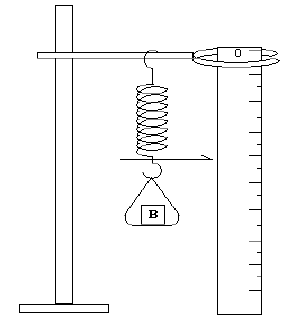
\includegraphics{./img/spring-practical.png}
\end{center}

\begin{itemize}
\item[]
\begin{itemize}
\item[(i)] Set up the apparatus as shown in the figure with zero mark of the metre-rule at the top of the rule and record the scale reading by the pointer, $S_0$.
\item[(ii)] Place the object ``B'' and standard weight (mass) W equal to 20 g in the pan and record the new pointer reading $S_1$. Calculate the extension, $e = S_1 - S_0$ in cm.
\item[(iii)] Repeat the procedure in (ii) above with W = 40 g, 60 g, 80 g and 100 g.
\end{itemize}
\item[(a)] Record your results in tabular form as shown below:\\
Table of Results:

\begin{tabular}{|p{2cm}|p{3cm}|p{3cm}|p{3cm}|}\cline{1-1}
\multicolumn{1}{|p{2cm}|}{$S_0 = $}&\multicolumn{2}{c}{} & \multicolumn{1}{p{2.5cm}}{} \\ \hline
\multicolumn{1}{|c|}{Mass} & \multicolumn{1}{c|}{Force, F (N)} & \multicolumn{1}{c|}{Pointer reading $S_1$} & \multicolumn{1}{c|}{Extension}\\
\multicolumn{1}{|c|}{(kg)} & \multicolumn{1}{c|}{} & \multicolumn{1}{c|}{(cm)} & \multicolumn{1}{c|}{$= S_1 - S_0$ (cm)}\\ \hline
\multicolumn{1}{|c|}{0} & \multicolumn{1}{c|}{} & \multicolumn{1}{c|}{} & \multicolumn{1}{c|}{}\\ 
\multicolumn{1}{|c|}{0.02} & \multicolumn{1}{c|}{} & \multicolumn{1}{c|}{} & \multicolumn{1}{c|}{}\\ 
\multicolumn{1}{|c|}{0.04} & \multicolumn{1}{c|}{} & \multicolumn{1}{c|}{} & \multicolumn{1}{c|}{}\\ 
\multicolumn{1}{|c|}{0.06} & \multicolumn{1}{c|}{} & \multicolumn{1}{c|}{} & \multicolumn{1}{c|}{}\\ 
\multicolumn{1}{|c|}{0.08} & \multicolumn{1}{c|}{} & \multicolumn{1}{c|}{} & \multicolumn{1}{c|}{}\\ 
\multicolumn{1}{|c|}{0.10} & \multicolumn{1}{c|}{} & \multicolumn{1}{c|}{} & \multicolumn{1}{c|}{}\\ \hline
\end{tabular}
\item[(b)] Plot graph of Force F (vertical axis) against extension $e$ (horizontal axis).
\item[(c)] Use your graph to evaluate
\begin{itemize}
\item[(i)] mass of B
\item[(ii)] spring constant, K, given that force, extension, constant and weight of B are related as follows:\\
F = K$e$ - B
\end{itemize}
\end{itemize}

%The aim of this experiment is to determine the mass of a given object $B$, and the
%constant of the spring provided.
%
%\begin{center}
%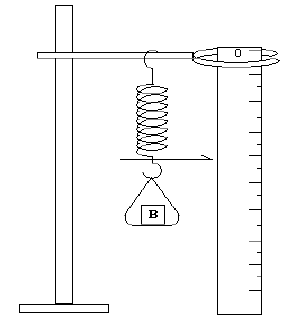
\includegraphics{./img/spring-practical.png}
%\end{center}
%
%\begin{enumerate}
%\item{Set up the apparatus as shown with the zero mark of the meter-rule at the top
%of the rule and record the scale reading, as shown by the pointer, $S_0$.}
%\item{Place the object $B$ and standard weight (mass) $W$ equal to 20~g in the pan
%and record the new pointer reading, $S_1$. Calculate the extension, $e = S_1 - S_0$ in
%cm.}
%\item{Repeat the procedure above with $W$ = 40~g, 60~g, 80~g and 100~g.}
%\item{Record your results in tabular form as shown below:
%
%\begin{center}
%\begin{tabular}{ | c | c | c | c | c | }
%\hline
%$S_0$ & Mass (kg) & Force, $F$ (N) & Pointer Reading $S_1$ (cm) & Extension, $e = S_1 - S_0$ (cm) \\ \hline
%& 0 & & & \\ \hline
%& 0.02 & & & \\ \hline
%& 0.04 & & & \\ \hline
%& 0.06 & & & \\ \hline
%& 0.08 & & & \\ \hline
%& 0.1 & & & \\ \hline
%\end{tabular}
%\end{center}
%
%}%Record your results...
%\item{Plot a graph of force $F$ (vertical axis) against extension $e$ (horizontal axis).}
%\item{Use your graph to evaluate
%\begin{enumerate}
%\item{mass of $B$}
%\item{spring constant, $K$, given that the force, extension, constant and
%weight of $B$ are related as follows: $$F = Ke - B$$}
%\end{enumerate}
%}%Use your graph...
%\end{enumerate}

\subsubsection{Discussion}

This practical has two parts: the first is to find the spring constant $k$, the second is
to find the mass of an unknown object $B$. By looking at the equation above, we
can see that $F$ is the dependent variable, $e$ is the independent variable, $K$ is the slope and
$-B$ is the intercept. When the graph is drawn, $K$ and $B$ can be found easily. Note that the
intercept on the graph will be negative.

The procedure is simply to start from a certain point on the metre rule (it does not
need to be a specific number) and to add masses one at a time, measuring the distance
from your starting point to the new position. This distance is called the extension, $e$. Be
sure that you are not simply reading the metre rule, but are measuring the distance from
the starting point.

\subsection{Simple Pendulum (Form 2)}

With some practice, this experiment should be simple for anyone to perform. The
trick comes with the math and graphing (again, an example is shown below). The
materials can all be local (string, stones, ruler) except for the stopwatches (for which you
should consult the materials section).

The practical usually has one objective: to find the acceleration due to gravity, $g$.
We know that the mass of a pendulum and its angle of deflection (for small angles) do
not affect its period. Therefore we vary only the length $L$ of the pendulum and measure
its period, as shown in the following example question.

\subsubsection{Sample Practical Question}

The aim of this experiment is to determine the magnitude of the acceleration due to
gravity, $g$. Proceed as follows:

\begin{center}
\includegraphics{./img/pendulum.png}
\end{center}


\begin{enumerate}
\item{Make a simple pendulum by suspending a weight on a string 10~cm long from a retort
stand.}
\item{Allow the pendulum to swing for twenty oscillations, using a stopwatch to record the
time. Repeat this procedure for pendulum lengths of 20~cm, 30~cm, 40~cm, and 50~cm.}
\item{Record your results in tabular form as shown below}

\begin{center}
\begin{tabular}{ | c | c | c | c | }
\hline
Pendulum Length l (m) & Time for 20 oscillations (s) & Period $T = \frac{t}{20}$ (s) & $T^2$ ($s^2$) \\ \hline
0.1 & & & \\ \hline
0.2 & & & \\ \hline
0.3 & & & \\ \hline
0.4 & & & \\ \hline
0.5 & & & \\ \hline
\end{tabular}
\end{center}

\item{Plot a graph of $T^2$ (vertical axis) against Pendulum Length (horizontal axis).}
\item{Calculate the slope of the graph.}
\item{Use the slope to calculate the value of $g$.}
\item{What are possible sources of error in this experiment?}

\end{enumerate}

\subsubsection{Discussion}

The period of a pendulum can be calculated using $$T = 2\pi\sqrt{\frac{l}{g}}$$
where $l$ is the length of the pendulum, $T$ is the period and $g$ is the acceleration due to
gravity. By squaring both sides, we get a much easier equation to graph: $$T^2 = 4\pi\frac{l}{g}$$ In this equation we see that $T^2$ is the dependent variable (y-axis) and $l$ is the
independent variable (x-axis), so the slope must be $$\mathrm{slope} = \frac{4\pi}{g}$$ 
When the graph is complete, the value of $g$ can be calculated easily.

Many students are confused by the difference between the time for many oscillations and
the period, which is the time for one oscillation. Be sure that they can change between
the two easily.

Note that pendulum practicals do not always require students to find $g$. Sometimes they are just required to find the relationship between $l$ and $t$. Again, it is essential that students read and understand the examination question, rather than memorize past solutions, and that they have lots of practice in collecting, organizing, and graphing data from a variety of experiments.

\subsection{Principle of Moments (Form 2)}

This experiment is used to verify the Principle of Moments, or equilibrium, by
balancing a meter rule on a knife-edge with masses at various distances. For this experiment, students need
a solid understanding of the Center of Gravity, the Moment of a force, and equilibrium.
Questions can range from finding the mass of an object to asking for
the mass of the metre rule. They are all
variations on the same practical: using the condition of equilibrium to find mass.

The following example is from the 2011 NECTA exam and asks students to find the mass of a battery using the Principle of Moments. Following is a brief explanation of the alternative practical of finding the mass of a metre rule.

\subsubsection{Finding the Mass of an Object}

\noindent \textbf{Sample Practical Question}\\

\noindent The aim of this experiment is to determine the mass of a given dry cell size ``AA''. Proceed as follows:
\begin{itemize}
\item[(a)] Locate and note the centre of gravity $C$ of the metre rule by balancing it on the knife edge.
\item[(b)] Suspend the 50 g mass at length `$a$' cm on one side of the metre rule and the 20 g mass together with the dry cell at length `$b$' cm on the other side of the metre rule. Fix the 50 g mass at length 30 cm from the fulcrum and adjust the position of the 20 g mass together with the dry cell until the metre rule balances horizontally. Read and record the values of $a$ and $b$ as $a_0$ and $b_0$ respectively.
\item[(c)] Draw the diagram for this experiment.
\item[(d)] By fixing $a = 5$ cm from fulcrum $C$, find its corresponding length $b$.
\item[(e)] Repeat the procedure in (d) above for $a = 10$ cm, 15 cm, 20 cm and 25 cm. Tabulate your results.
\item[(f)] Draw a graph of `$a$' against `$b$' and calculate its slope $G$.
\item[(g)] Calculate $X$ from the equation $50 = \cfrac{b_0}{a_0}(20 + X)$.
\item[(h)] Comment on the value of $\cfrac{b_0}{a_0}$.
\item[(i)] Sate the principle governing this experiment.
\end{itemize}

\noindent \textbf{Discussion}\\
This practical utilizes the Principle of Moments to find the mass of a ``AA'' battery. Initially, a known mass of 50 g is balanced with the (battery $+$ 20 g mass) system. Note that `$a$' and `$b$' are measured \emph{from the fulcrum} and so students should be careful not to just read the cm mark on the ruler where each object is suspended.

Also note that students are required to actually find the centre of gravity $C$ of the ruler rather than assuming it to be the 50 cm mark. This measured value of $C$ is to be used as the starting point for all future measurements of $a$ and $b$.

In part (g), students should recognize the equation $50 = \cfrac{b_0}{a_0}(20 + X)$ as coming from the Principle of Moments. Starting with
$$F_{\mathrm{clockwise}} \times d_{\mathrm{clockwise}} = F_{\mathrm{anticlockwise}} \times d_{\mathrm{anticlockwise}}$$
we get $$(mg)_{\mathrm{clockwise}} \times d_{\mathrm{clockwise}} = (mg)_{\mathrm{anticlockwise}} \times d_{\mathrm{anticlockwise}}$$
or $$(50 \text{g})(g) \times a_0 \text{ cm} = (20 \text{g} + X \text{g})(g) \times b_0 \text{ cm}$$
Canceling $g$ and dividing by $a_0$ reveals
$$50 = \cfrac{b_0}{a_0}(20 + X)$$
where $\cfrac{b_0}{a_0}$ is the ratio of the lever arm distances for the two weights being used. If the mass of the battery $X$ is less than 30 g, this ratio should be greater than 1, but if the mass is greater than 30 g, the ratio should be less than 1.

\subsubsection{Finding the Mass of a Metre Rule}

This question is less frequently seen on NECTA exams as compared to finding an unknown mass. However, it utilizes the same principles of equilibrium and balancing moments, and therefore is a useful alternative practical to ensure that students understand the concept rather than memorizing solutions to one version of the problem.

The mass of a uniform solid object, like a metre rule, is assumed to be at the
center of the object. In the case of the metre rule, we can say that the center of mass is at
the 50~cm mark, directly in the center. If we want it to be in equilibrium, the moments on
either side of a pivot must be equal, or $$ \mathrm{\text{Clockwise moment}} = \mathrm{\text{Anticlockwise moment}}$$
To find the mass of the metre rule itself, we begin by placing a known mass at one
point on the metre rule. We then move the pivot to one side or another until the metre
rule is perfectly balanced in equilibrium. As shown in the diagram below, the pivot will
not be at the 50~cm mark.

\begin{center}
\includegraphics{./img/meter-rule.png}
\end{center}

If the metre rule is in equilibrium, we know that the moments must be equal, or
that $$F_{\mathrm{clockwise}} \times d_{\mathrm{clockwise}} = F_{\mathrm{anticlockwise}} \times d_{\mathrm{anticlockwise}}$$
In this case, the anticlockwise force is the weight of the object, and the distance is that
from the pivot to the object. The clockwise force is the weight of the metre rule, and the
distance is that from the 50~cm mark (center of mass) to the pivot. Therefore our
equation is: $$ W_{\mathrm{rule}} \times d_{\mathrm{rule}} = W_{\mathrm{object}} \times d_{\mathrm{object}} $$
Because the weight of the object is known, and the two distances can be measured, we
can easily calculate the mass and therefore the weight of the metre rule:
$$W_{\mathrm{rule}} = \frac{W_{\mathrm{object}} \times d_{\mathrm{object}}}{d_{\mathrm{rule}}}$$
From this we can calculate mass of the metre rule using $F = mg$.

%==============================================================================
\section{Light}
The light practical typically involves plane mirrors or glass blocks (rectangular
prisms). Presumably you will have already done these practicals with the students in Form
three (refraction) and Form 1 (plane mirrors), but a little practice will make the theory and
execution clear, especially if they can work in groups. The materials you will need are as
follows:
\begin{description}
\item[Cork Board]{Use cardboard for this, about 0.5 to 0.75~cm thick.}
\item[Optical pins]{Use sewing pins or syringe needles. If using syringe needs, be
sure to crimp the ends so students do not prick themselves.}
\item[Protractors]{These are cheap and students are supposed to have them anyway.
Small ones come in local mathematical sets.}
\item[Glass Block / Rectangular Prism]{A simple rectangular piece of 6~mm glass,
about 8~cm by 12~cm, will work.}
\item[Plane Mirror]{You can buy mirror glass in town in small sections for 200/= or
less; it should be available in villages through the local craftsmen if they work on
windows. Alternately, you can smoke one side of a piece of glass to make the
other side like a mirror.}
\end{description}

\subsection{Plane Mirror (Reflection) (Form 1)}

These are not as common as the rectangular prism, but they come in a variety of
questions:
\begin{itemize}
\item{Placing pins in front of a mirror at different distances and finding the distance of
the image.}
\item{Verifying the Law of Reflection at plane mirrors.}
\item{Placing two mirrors at different relative angles to find the number of images
produced.}
\end{itemize}
These are not overly complicated, but you should definitely practice with your students creating images in
mirrors -- they are not as accustomed to playing with mirrors as you might be.

Given below is an example practical from the 2006 NECTA exam which asks students to find a relationship between object distance and image distance in a plane mirror.

\subsubsection{Sample Practical Question}

Set up the experiment as shown in the diagram below using plane mirror, soft board, three pins and a white sheet of paper.

\begin{center}
\includegraphics[width=8cm]{./img/2006-2-alt.png}
\end{center}

Fix a white sheet of paper on the soft board. Draw a line across the width at about the middle of the white sheep (MP). Draw line ONI perpendicular to MP.

Fix optical pin O to make ON = U = 3 cm. By using plasticine or otherwise, fix plane mirror along portion of MP with O in front of the mirror. With convenient position of eye, E, look into the mirror and fix optical pins A and B to be in line with image, I, of pin O.

Measure and record NI = V. Repeat procedure for U = 6 cm, 9 cm and 12 cm.

\begin{enumerate}
\item[]
\begin{enumerate}
\item[(a)] Tabulate your results as follows:

\quad \begin{tabular}{|c|c|c|c|c|} \hline
U (cm) & 3 & 6 & 9 & 12 \\ \hline
V (cm) & & & & \\ \hline
\end{tabular}

\item[(b)] Plot graph of U against V.
\item[(c)] Calculate slope, $m$ of the graph to the nearest whole number.
\item[(d)] State relationship between U and V.
\item[(e)] Write equation connecting U and V using numerical value of $m$ with symbols U and V.
\item[(f)] From your equation give position of the image when object is touching the face of the mirror.
\end{enumerate}
\end{enumerate}

\subsubsection{Discussion}
For a plane mirror, object distance and image distance are equal. That is, U and V should be approximately equal values for this practical. Note that students should extend line ONI far behind the mirror since they don't know where exactly the image I is going to be. The location of I is found at the intersection of the extended line ONI and the extended line AB connecting the two optical pins.

From the graph, the slope should be found to be 1 after rounding to the nearest whole number. From this, we can see that U = V. When the object is touching the face of the mirror, the object distance U is 0, and so the image distance V will also be 0.

\subsection{Rectangular Prism (Refraction) (Form 3)}

Students will be asked to find the refractive index and/or critical angle of the glass block by varying
the angle of incidence $i$ and measuring the corresponding angles of refraction $r$ as
described in the Mathematics section earlier. They will do this by placing two pins in
front of the prism, which together form a `ray' (the light ray), and then placing two more
pins on the other side of the prism so that, when observed through the prism from either
side, the four pins line up exactly. By drawing the lines that the pins make on the paper,
the refracted ray inside the prism can be easily traced, and the refracted angle measured.
An example question from the 2007 NECTA is given below.

\subsubsection{Sample Practical Question}

The aim of this experiment is to find the refractive index of a glass block. Proceed
as follows:\\

Place the given glass block in the middle of the drawing paper on the drawing
board. Draw lines along the upper and lower edges of the glass block. Remove the
glass block and extend the lines you have drawn. Represent the ends of these line
segments as $SS_1$ and $TT_1$. Draw the normal $NN_1$ to the parallel lines $SS_1$ and
$TT_1$ as shown in the figure below:

\begin{center}
\includegraphics{./img/light-block-1.png}
\end{center}

Draw five evenly spaced lines from O to represent incident rays at different
angles of incidence (10$^\circ$, 20$^\circ$, 30$^\circ$, 40$^\circ$, and 50$^\circ$ from the normal). Replace the
glass block carefully between $SS_1$ and $TT_1$. Stick two pins $P_1$ and $P_2$ as shown in
the figure as far apart as possible along one of the lines drawn to represent an
incident ray. Locate an emergent ray by looking through the block and stick pins
$P_3$ and $P_4$ exactly in line with images $I_1$ and $I_2$ of pins $P_1$ and $P_2$. Draw the
emergent ray and repeat the procedure for all the incident rays you have drawn. Finally draw in the corresponding refracted rays.

\begin{center}
\includegraphics{./img/light-block-2.png}
\end{center}

\begin{enumerate}
\item[]
\begin{enumerate}
\item[(a)]{Record the angles of incidence $i$ and the measured corresponding angles of
refraction $r$ in a table. Your table of results should include the values of
$\sin{i}$ and $\sin{r}$.}
\item[(b)]{Plot the graph of $\sin{i}$ (vertical axis) against $\sin{r}$ (horizontal axis).}
\item[(c)]{Determine the slope of the graph.}
\item[(d)]{What is the refractive index of the glass block used?}
\item[(e)]{Mention any sources of errors in this experiment.}
\end{enumerate}
\end{enumerate}

\subsubsection{Discussion}

In this experiment, pins are used to simulate a ray of light. If all of the pins are
aligned as you look through the block, they act as a single ray. It takes practice to be able
to align the pins while looking through the block, so practice often with your students.

Light slows down as it enters a denser medium, so in order to minimize the time
required to pass through that medium, it changes direction until it moves back into its
original medium. In this case, light is moving from air into glass and then back into air,
so its direction changes while inside the glass, then returns to its original direction when
passing back into air. This effect is called refraction and it depends on the nature of the
media, in this case air and glass. Snell’s law gives us the relationship between the nature
of the media and the resulting angles of incidence and refraction:
$$n_1 \times \sin{i} = n_2 \times \sin{r}$$

In this experiment, the incident angle $i$ is being changed and the refracted angle $r$
is being measured. The refractive index of medium 1 (air) is known as 1.0, so we can use
these three to find the refractive index of medium 2 (glass). On the graph, $\sin{i}$ is the
dependent variable and $\sin{r}$ is the independent variable, so the equation becomes
$$\sin{i} = \sin{r} \frac{n_2}{n_1}$$
In this case the slope must be $\frac{n_2}{n_1}$.

The refractive index of medium air is simply 1.0, so the slope is the refractive index of
medium 2.

This practical is one of the easiest to perform with students because it does not
require much preparation. Syringe needles should be readily available and glass blocks are
cheap, so it is possible to have every students try this themselves many times before
taking the exam.

\subsubsection{Finding the Critical Angle}
Some questions may ask students to find the critical angle of a glass block in addition to its refractive index. The relationship between critical angle, $C$, and refractive index, $n$, for a particular medium is given by 
$$n = \frac{1}{\sin{C}}$$ or $$\frac{\sin{i}}{\sin{r}} = \frac{1}{\sin{C}}$$.

Thus a graph of $\sin{i}$ against $\sin{r}$ can be used to find the critical angle. However, take care to note that we must first take the reciprocal of the slope, i.e.
$$\sin{C} = \frac{1}{n}$$.

This gives us $\sin{C}$, so to get $C$ by itself, we need to use mathematical tables. Turn to the page for Natural Sines and search the table for the 4-figure value you obtained above by taking $\frac{1}{\text{slope}}$. The corresponding row gives the angle in degrees and the column gives the additional minutes of the angle.

For example, say we plot our graph of $\sin{i}$ ($y$-axis) against $\sin{r}$ ($x$-axis) and we calculate the slope to be 1.43. This is the refractive index of the glass block (since we can remember that glass has a refractive index of 1.5, we can do a quick mental check to make sure this makes sense). Then $\sin{C} = \frac{1}{1.43} = 0.6993$. From the mathematical tables, we get $C = 44^\circ 22'$ [6993 falls between 6984 ($18'$) and 6997 ($24'$), so we use the Mean Differences table to add on $4'$ giving a total of $22'$].

Note that the method of finding $n$ and $C$ changes if we are instead told to graph $\sin{r}$ ($y$-axis) against $\sin{i}$ ($x$-axis). Be sure to practice both versions with students to ensure their understanding.

%==============================================================================
\section{Electricity}

This is by far the least attempted practical on the exam, but not because it is
difficult. The electricity practical, if properly set up, is one of the easiest to perform. It
can appear in many different forms but will typically involve a simple circuit and some
kind of variable resistor in order to measure current or EMF for different resistances. The
materials you will probably need are as follows:

\begin{description}
\item[Connecting Wires]{Use speaker wire; it is cheap and available in most villages
and towns.}
\item[Voltmeters, Ammeters, Galvanometers]{This is unavoidable; you can get full
digital multimeters in town for about 10,000/=, galvanometers can be found in
any lab store or can be made using a compass and insulated copper wire.}
\item[Batteries]{Two to four D-size batteries should easily be enough for these experiments. Try to avoid Tiger brand if possible. Panasonic is highly superior in quality for roughly the same price.}
\item[Resistance Wire]{These are used to make small resistors for
the metre bridge or potentiometer. The most common type of wire to use is
nichrome, which can be found in a hardware or lab store. Steel will also work, though it
is less resistant and therefore harder to measure.}
\item[Metre Bridges]{See the activity that describes the construction of a metre bridge
and potentiometer. It is best to make both together as the construction is almost
identical and both are used frequently.}
\item[Variable Resistor (Rheostat)]{This is optional as it is typically only used to set a
level that can be easily read by the voltmeter. However, if you are using a
multimeter, you can simply change the magnitude setting on the multimeter to
account for unusually low or high resistances.}
%See How to Use a Rheostat
\item[Soldering Iron]{Not required, but may be a good investment for making reliable battery connections. Using electrical tape can lead to inconsistencies. Check large towns, prices should range from 10,000/= to 20,000/=.}
\end{description}

\subsection{Potentiometers (Form 3)}

This experiment is very simple but requires the correct materials, namely the
meter bridge/potentiometer described above. A complete circuit is created with a switch
(optional), power source, variable resistor and 1~m of bare resistance wire, all in series.

The potentiometer itself is simple to construct; all preparation is done by the teacher, so
the student simply follows the instructions as shown in the following example from the 2007 NECTA.

\subsubsection{Sample Practical Question}

The aim of this experiment is to determine the potential fall along a uniform
resistance wire carrying a steady current. Proceed as follows:

\begin{center}
\includegraphics[width=10cm]{./img/meter-bridge-1.png}
\end{center}


Connect up the circuit as shown in the figure. Adjust the rheostat so that when the sliding
contact J is near B and the key is closed the voltmeter V indicates an almost full scale
of deflection. Do not alter the rheostat again.

Close key K and make contact with J, so that AJ = 10~cm. Record the potential
difference V volts between A and J as registered on the voltmeter.

Repeat this procedure for AJ = 20~cm, 30~cm, 50~cm, and 70~cm.

\begin{enumerate}
\item[]
\begin{enumerate}
\item[(a)]{Tabulate your results for the values of AJ and V.}
\item[(b)]{Plot a graph of V (vertical axis) against AJ (horizontal axis).}
\item[(c)]{Calculate the slope of the graph.}
\item[(d)]{What is your comment on the slope?}
\item[(e)]{State any precautions on the experiment.}
\end{enumerate}
\end{enumerate}

\subsubsection{Discussion}

This is a simple test of the relationship between the length of a wire and its
resistance, which we know is $$R=\frac{\rho l}{A} $$

Where $l$ is the length of the wire, $\rho$ is the resistivity of the wire, and $A$ is the cross-sectional
area of the wire. We expect that as the length of wire increases, its potential difference
will also increase. This is because the resistance (and therefore potential difference) of a wire is
directly related to its length. The voltmeter in this experiment is measuring just the
potential difference over the length of wire (10~cm, 20~cm, etc.), so if we use Ohm’s Law to say that $V = IR$, we can write:\\
$$ V = \frac{I \rho l}{A} $$
In this experiment, $I$, $\rho$ and $A$ are all constant, so the slope is
$$\mathrm{slope} = \frac{I \rho}{A} $$
Though it is not asked for directly in the question, we can find the resistivity, $\rho$, by measuring $I$ with an ammeter/galvanometer and $A$ with vernier calipers or a micrometer screw gauge.

\subsection{Metre Bridges (Form 3)}

A metre bridge resembles a potentiometer, except that it uses a galvanometer to
measure the difference in current between two points on the circuit, hence the name
``bridge.'' The same materials can be used as with the potentiometer, though it is best to
use small coils of resistance wire for the small resistors (between 3$\Omega$ and 20$\Omega$ is a good resistance). A galvanometer can be made easily if one is not available.

\begin{center}
\includegraphics[width=10cm]{./img/meter-bridge-2.png}
\end{center}

Resistors $R_1$ and $R_2$ have different resistances, but they should be somehow similar so
that one resistor does not take all of the current (this will make it difficult to measure the
length to the galvanometer). About 5$\Omega$ and 10$\Omega$, for example, would work well.

However, for the sake of the practical, one resistor should not be known; the objective of
the practical is to find the unknown resistance. The long wire along the bottom edge is a
metre of nichrome wire or other resistance wire. One terminal of the galvanometer is
connected between the two resistors, and the other terminal is connected to a flying wire (or jockey)
that is free to move along the length of the nichrome wire.

The practical instructs you to move the galvanometer's flying wire back and forth
along the nichrome wire until it reads zero. At this point, we know that no current is
passing through the galvanometer, so the potential difference across it is zero. This
means that the current flowing through $R_1$ is the same as that current flowing through $R_2$,
and the current flowing through the nichrome wire is constant. From this we can
conclude that
$$ \frac{R_1}{L_1} = \frac{R_2}{L_2} $$
or that the ratio of the two resistors is equal to the ratio of distances from the flying wire
to either end of the nichrome wire. The resistance of one resistor (say, $R_1$) is known and
the lengths $L_1$ and $L_2$ can be measured from the flying wire to either side of the
nichrome wire. Using the ratio above, we can easily calculate the unknown resistance $R_2$.

An example is given below from the 2006 NECTA exam.

\subsubsection{Sample Practical Question}
You are required to determine the unknown resistance labeled X using a metre bridge circuit. Connect your circuit as shown below, where $R$ is a resistance box, G is a galvanometer, J is a jockey and others are common circuit components.

\begin{center}
\includegraphics[width=12cm]{./img/2006-3-alt.png}
\end{center}

Procedure:\\

With $R$ = 1 $\Omega$, obtain a balance point on a metre bridge wire AB using a jockey J. Note the length $l$ in centimetres. Repeat the experiment with R equal to 2 $\Omega$, 4 $\Omega$, 7 $\Omega$ and 10 $\Omega$.\\

Tabulate your results for $R$, $l$ and $^1/_l$.

\begin{itemize}
\item[(a)]
\begin{itemize}
\item[(i)] Plot a graph of $R$ (vertical axis) against $^1/_l$ (horizontal axis).
\item[(ii)] Determine the slope S of your graph.
\item[(iii)] Using your graph, find the value of $R$ for which $^1/_l = 0.02$.
\end{itemize}
\item[(b)] Read and record the intercept $R_0$ on the vertical axis.
\item[(c)] Given that,\\
\quad \quad $R = \cfrac{100 \text{X}}{l} - \text{X}$\\
Use the equation and your graph to determine the value of X.
\item[(d)] Comment on your results in (a)(iii), (b) and (c) above.
\end{itemize}

\subsubsection{Discussion}
The procedure for this question is similar to most other wheatstone bridge problems: vary a known resistor and see how it affects the relative lengths in resistance wire required to balance the potential difference and give no current through the galvanometer. It may not be obvious at first, however, where the equation $R = \frac{100 \text{X}}{l}$ - X comes from.

Starting with the balancing ratio for a wheatstone bridge, $$ \frac{R_1}{L_1} = \frac{R_2}{L_2} $$ we can solve for the unknown resistor $$R_2 = R_1\left(\frac{L_2}{L_1}\right)$$. 

Recall that $L_1$ and $L_2$ are the corresponding lengths from either end of the metre rule to the jockey (in cm), and so taking them together, we get $$L_1 + L_2 = 100$$. Dividing both sides by $L_1$ gives $$1 + \frac{L_2}{L_1} = \frac{100}{L_1}$$. Then solving for $\frac{L_2}{L_1}$, $$\frac{L_2}{L_1} = \frac{100}{L_1} - 1$$. Now substitute this into our previous equation for $R_2$: $$R_2 = R_1\left(\frac{100}{L_1} - 1\right)$$. Replacing $R_2$ with $R$, $L_1$ with $l$ and $R_1$ with X for this problem and distributing gives, $$R = \frac{100 \text{X}}{l} - \text{X}$$.

From this equation, we have dependent variable $R$, independent variable $\frac{1}{l}$, slope $100 \text{X}$ and $y$-intercept $-\text{X}$. So we can obtain the value of the unknown resistor X either by using the $y$-intercept (note the resistance is a positive value) or by taking the slope divided by 100.

\subsection{Ohm’s Law (Form 2)}

The practical may give any kind of experiment to use or verify Ohm’s Law in a
simple circuit. Finding the e.m.f. and internal resistance of cells appears frequently. Students should be very familiar with the law, as well as the factors that determine resistance in a wire and the effect of internal resistance of a cell on a circuit. Given below is an example problem taken from the 2011 NECTA exam.

\subsubsection{Sample Practical Question}
You are provided with an ammeter, A, resistance box, R, dry cell, D, a key, K and connecting wires. Proceed as follows:
\begin{enumerate}
\item[]
\begin{enumerate}
\item[(a)] Connect the circuit in series.
\item[(b)] Put $R$ = 1 $\Omega$ and quickly read the value of current $I$ on the ammeter.
\item[(c)] Repeat procedure (b) above for $R$ = 2 $\Omega$, 3 $\Omega$, 4 $\Omega$ and 5 $\Omega$. Record your results in a tabular form.
\item[(d)] Draw the circuit diagram for this experiment.
\item[(e)] Plot the graph of $R$ against $\cfrac{1}{I}$.
\item[(f)] Determine the slope of the graph.
\item[(g)] If the graph obeys the equation $R=\cfrac{E}{I}-r$, then
\begin{enumerate}
\item[(i)] suggest how $E$ and $r$ may be evaluated from your graph.
\item[(ii)] compute $E$.
\item[(iii)] compute $r$.
\end{enumerate}
\item[(h)] State one source of error and suggest one way of minimizing it.
\item[(i)] Suggest the aim of this experiment.
\end{enumerate}
\end{enumerate}

\subsubsection{Discussion}
To see where the equation $R=\cfrac{E}{I}-r$ comes from, first start with Ohm's Law, $V = IR$. Accounting for the internal resistance of the cell, $r$, this becomes $$V = I(R + r)$$. To solve for resistance, we divide both sides by $I$, which gives $$(R + r) = \frac{V}{I}$$. From this we can see that, using $E$ as e.m.f. for this problem, $$R=\cfrac{E}{I}-r $$. 

In this form, the equation resembles the classic $y = mx + c$, where $R$ is the dependent variable, $\frac{1}{I}$ the independent variable, $E$ is the slope and $-r$ is the y-intercept (note the internal resistance is a positive value).

%\pagebreak
%
%\section{NECTA Past Papers}
%\setcounter{secnumdepth}{1}
%\subsection{2011 - PHYSICS 2A ACTUAL PRACTICAL A}

\begin{enumerate}
\item The aim of this experiment is to determine the mass of a given dry cell size ``AA''. Proceed as follows:
\begin{itemize}
\item[(a)] Locate and note the centre of gravity $C$ of the metre rule by balancing it on the knife edge.
\item[(b)] Suspend the 50 g mass at length `$a$' cm on one side of the metre rule and the 20 g mass together with the dry cell at length `$b$' cm on the other side of the metre rule. Fix the 50 g mass at length 30 cm from the fulcrum and adjust the position of the 20 g mass together with the dry cell until the metre rule balances horizontally. Read and record the values of $a$ and $b$ as $a_0$ and $b_0$ respectively.
\item[(c)] Draw the diagram for this experiment.
\item[(d)] By fixing $a = 5$ cm from fulcrum $C$, find its corresponding length $b$.
\item[(e)] Repeat the procedure in (d) above for $a = 10$ cm, 15 cm, 20 cm and 25 cm. Tabulate your results.
\item[(f)] Draw a graph of `$a$' against `$b$' and calculate its slope $G$.
\item[(g)] Calculate $X$ from the equation $50 = \cfrac{b_0}{a_0}(20 + X)$.
\item[(h)] Comment on the value of $\cfrac{b_0}{a_0}$.
\item[(i)] Sate the principle governing this experiment.
\end{itemize}
\end{enumerate}

\flushright \textbf{(25 marks)}
\begin{enumerate}
\item[2.] You are provided with an ammeter, A, resistance box, R, dry cell, D, a key, K and connecting wires. Proceed as follows:
\begin{enumerate}
\item[(a)] Connect the circuit in series.
\item[(b)] Put $R$ = 1 $\Omega$ and quickly read the value of current $I$ on the ammeter.
\item[(c)] Repeat procedure (b) above for $R$ = 2 $\Omega$, 3 $\Omega$, 4 $\Omega$ and 5 $\Omega$. Record your results in a tabular form.
\item[(d)] Draw the circuit diagram for this experiment.
\item[(e)] Plot the graph of $R$ against $\cfrac{1}{I}$.
\item[(f)] Determine the slope of the graph.
\item[(g)] If the graph obeys the equation $R=\cfrac{E}{I}-r$, then
\begin{enumerate}
\item[(i)] suggest how $E$ and $r$ may be evaluated from your graph.
\item[(ii)] compute $E$.
\item[(iii)] compute $r$.
\end{enumerate}
\item[(h)] State one source of error and suggest one way of minimizing it.
\item[(i)] Suggest the aim of this experiment.
\end{enumerate}

\end{enumerate}

\flushright \textbf{(25 marks)}
\flushleft
%\pagebreak
%\section{2010 - PHYSICS 2A ALTERNATIVE A PRACTICAL}

\begin{enumerate}
\item[1.] The aim of this experiment is to find the mass of the unknown load labeled ``$W$'' and the spring constant $K$. Proceed as follows:

\begin{center}
\includegraphics[width=14cm]{./img/2010-1-alt.png}
\end{center}

Set up the apparatus as shown in Figure 1. Put a mass of 50 g on the scale pan and record the equilibrium position $X_0$ of the pointer. Put on the scale pan the unknown weight marked $W$. Without removing $W$ and the 50 g mass in the scale pan, add a load $L$ of 50 g and record the new position of the pointer $X$. Calculate the extension $E = (X - X_0)$. Repeat this process for $L$ = 100 g, 150 g, 200 g and 250 g.
\begin{enumerate}
\item[(a)] Record you conclusions as shown in Table 1.\\[10pt]

Equilibrium position $X_0$..................\\[10pt]

Table 1\\[10pt]

%\begin{center}
\begin{tabular}{|p{3cm}|p{3cm}|p{3cm}|} \hline
\multicolumn{1}{|c|}{Load (g)} & \multicolumn{1}{c|}{$X$ (cm)} & \multicolumn{1}{c|}{$E = X - X_0$ (cm)} \\ \hline
\multicolumn{1}{|c|}{50} & & \\ \hline
\multicolumn{1}{|c|}{100} & & \\ \hline
\multicolumn{1}{|c|}{150} & & \\ \hline
\multicolumn{1}{|c|}{200} & & \\ \hline
\multicolumn{1}{|c|}{250} & & \\ \hline
\end{tabular}\\[10pt]
%\end{center}

\item[(b)] Plot the graph of load L against absolute value of extension E. The scale of the vertical axis should be chosen to range from 200 g to 300 g.
\item[(c)] From the graph, determine the unknown weight marked W, given that L = KE + W where K is a constant.
\item[(d)] What does the gradient of the graph represent?
\item[(e)] State the sources of errors and precautions that should be taken in the experiment.
\end{enumerate}
\end{enumerate}
\flushright \textbf{(25 marks)}

\pagebreak

\begin{enumerate}
\item[2.] The aim of this experiment is to determine the refractive index of water. Proceed as follows:

\begin{center}
\includegraphics[width=10cm]{./img/2010-2-alt.png}
\end{center}

\begin{enumerate}
\item[(a)] Arrange your apparatus as in Figure 2. Put about 150 cm$^3$ of clear water in the measuring cylinder. Drop an office pin at the bottom so that it rests touching the wall of the cylinder.
\item[(b)] Look in the cylinder from Figure 2. Use another office pin as a search pin, move it up and down outside the cylinder, and locate the image position by no parallax method. Locate the image position of the ruler. Measure and record the depth ($H_1$) of the image. Measure and record the depth ($H_2$) of water. Repeat the experiment with 175 cm$^3$, 200 cm$^3$, 225 cm$^3$ and 250 cm$^3$ of water in the measuring cylinder.
\item[(c)] 
\begin{enumerate}
\item[(i)] Record in Table 2 your values of $H_1$ and $H_2$ corresponding to the volumes of water in the measuring cylinder.\\[10pt]

Table 2\\[10pt]

%\begin{center}
\begin{tabular}{|p{3cm}|p{3cm}|p{3cm}|} \hline
\multicolumn{1}{|c|}{Volume of water V (cm)} & \multicolumn{1}{c|}{$H_1$} & \multicolumn{1}{c|}{$H_2$} \\ \hline
\multicolumn{1}{|c|}{150} & & \\ \hline
\multicolumn{1}{|c|}{175} & & \\ \hline
\multicolumn{1}{|c|}{200} & & \\ \hline
\multicolumn{1}{|c|}{225} & & \\ \hline
\multicolumn{1}{|c|}{250} & & \\ \hline
\end{tabular}\\[10pt]
%\end{center}

\item[(ii)] Plot the graph of $H_2$ versus $H_1$.
\item[(iii)] Determine the slope of the graph.
\item[(iv)] What is the physical meaning of the slope?
\item[(v)] State sources of error in this experiment.
\end{enumerate}
\end{enumerate}
\end{enumerate}
\flushright \textbf{(25 marks)}

\pagebreak

\begin{enumerate}
\item[3.] The aim of this experiment is to determine the resistivity of an electrical conductor $P$.

\begin{center}
\includegraphics[width=10cm]{./img/2010-3-alt.png}
\end{center}

With $P$ having a length $l = 50$ cm, connect up the circuit as shown in Figure 3. Close one key S and adjust the rheostat R so that the current in $P$ is 0.20 A. Record the current $I$ and the potential difference $V$ between its ends.\\[10pt]

Repeat the procedure with current $I = $0.30 A, 0.40 A, 0.50 A and 0.60 A.
\begin{enumerate}
\item[(a)] Record your results in Table 3.\\[10pt]

Table 3\\[10pt]

%\begin{center}
\begin{tabular}{|p{3cm}|p{3cm}|} \hline
\multicolumn{1}{|c|}{Current $I$ (A)} & \multicolumn{1}{c|}{P.d. (volts)} \\ \hline
\multicolumn{1}{|c|}{0.20} &  \\ \hline
\multicolumn{1}{|c|}{0.30} &  \\ \hline
\multicolumn{1}{|c|}{0.40} &  \\ \hline
\multicolumn{1}{|c|}{0.50} &  \\ \hline
\multicolumn{1}{|c|}{0.60} &  \\ \hline
\end{tabular}\\[10pt]
%\end{center}

\item[(b)] Plot a graph of $V$ against $I$ and calculate the slope $G$.
\item[(c)] Deduce the resistivity of the conductor $P$ given that; $\rho = \cfrac{G\pi d^2}{4l}$.\\[10pt]
Where $\rho$ = resistivity\\
$d$ = diameter of $P$ (measured using the micrometer screw gauge provided).
\end{enumerate}
\end{enumerate}

\flushright \textbf{(25 marks)}
\flushleft
%\pagebreak
%\subsection{2009 - PHYSICS 2A ALTERNATIVE A PRACTICAL}

\begin{enumerate}
\item[1.] In this experiment you are required to find the relationship between the length of a simple pendulum and its period. Proceed as follows:
\begin{itemize}
\item[(a)] Suspend a simple pendulum of length L = 100 cm. Displace the pendulum through a small angle so that it swings parallel to the edge of the bench or table, determine the time for 20 oscillations. Continue reducing the length of the pendulum by 10 cm each time and obtain a total of six readings.
\item[(b)] Record your readings in a table as shown below.


\begin{tabular}{|p{2.5cm}|p{2.5cm}|p{2.5cm}|p{2.5cm}|p{2.5cm}|} \hline
Length of pendulum L (cm) & Log$_{10}$L & Time for 20 oscillations & Period T & Log$_{10}$T \\ \hline
&&&& \\ 
&&&& \\ 
&&&& \\ 
&&&& \\ 
&&&& \\ 
&&&& \\ 
&&&& \\ 
&&&& \\ \hline
\end{tabular}\\[10pt]

\noindent Assuming that T $ \propto $ L$^a$, we have T = $k$L$^a$ and taking logarithms to base ten on both sides we get $\log_{10}$T = $a\log_{10}$L + $\log_{10}k$.

\begin{itemize}
\item[(i)] Plot a graph of $\log_{10}$T (vertical axis) against $\log_{10}$L (horizontal axis) hence determine the values of $a$ and $k$ each correct to one decimal place.
\item[(ii)] From your answer in (i) above write down the values of $a$ and $k$ each in the form of $\cfrac{b}{c}$ where $b$ and $c$ are integers (i.e. whole numbers).
\item[(iii)] From the assumption and your answer in (ii) deduce the form of the equation governing the motion of the simple pendulum.
\end{itemize}

\end{itemize}
\end{enumerate}
\flushright \textbf{(25 marks)}


\begin{enumerate}
\item[2.] The aim of this experiment is to determine the refractive index $\eta$ of a given glass block.

\begin{center}
\includegraphics[width=8cm]{./img/2009-2-alt.png}
\end{center}

Place the rectangular glass block on the white paper on a drawing board. Using a pencil trace the outline of the block. Remove the glass block and draw a normal NOM near the left end of the block (Figure 1).\\[10pt]

\noindent Using a protractor and a pencil measure $\theta = 20^\circ$, draw a line making the angle $20^\circ$ with the surface RR of the block. Erect two pins T$_1$ and T$_2$ on this line and at a suitable distance from one another. Return the block and erect the pins T$_3$ and T$_4$ at positions such that they lie in a straight line with pins T$_1$ and T$_2$ as seen through the block. Now remove the block and draw a complete path of the ray (Figure 1).\\[10pt]

\noindent Measure the length MN$'$ and ON$'$: Repeat the procedure for values of $\theta = 30^\circ, 40^\circ$ and $60^\circ$ respectively. In each case make a drawing on a fresh part of the drawing paper.

\begin{itemize}
\item[(a)] Record the values of $\theta$, MN$'$, ON$'$, $\cfrac{\text{MN}'}{\text{ON}'}$ and $\cos \theta$ in a tabular form.
\item[(b)] Plot a graph of $\cfrac{\text{MN}'}{\text{ON}'}$ against $\cos \theta$.
\item[(c)] Find the slope $G$ of the graph.
\item[(d)] Calculate the value of the refractive index $\eta$; given that $G = \cfrac{1}{\eta}$.
\item[(e)] State two sources of errors. \hfill \textbf{(25 marks)}
\end{itemize}

\end{enumerate}


\begin{enumerate}
\item[3.] The aim of this experiment is to verify Ohm's Law.

\begin{center}
\includegraphics[width=7cm]{./img/2009-3-alt.png}
\end{center}

\begin{itemize}
\item[(a)] Set up the apparatus as shown on Figure 2, close switch S. Adjust the Rheostat Rh by sliding slowly from one end, read and record the value V of the voltmeter and current I of the ammeter.
\item[(b)] Repeat the experiment by changing the Rheostat slider to obtain about five pair of readings.\\[10pt]

\textbf{NB:} Adjust the Rheostat until when the pointer is exactly on the division of the metre scale.\\[10pt]

Table of results\\[10pt]
\begin{tabular}{|c|c|c|c|c|c|c|c|}\hline
V (V)&&&&&&&\\ \hline
I (A)&&&&&&& \\ \hline
\end{tabular}

\item[(c)] Plot a graph of V (vertical axis) against I (horizontal axis).
\item[(d)] 
\begin{itemize}
\item[(i)] Find the slope of the graph.
\item[(ii)] What is the relation between V and I?
\item[(iii)] Find the resistance R. \hfill \textbf{(25 marks)}
\end{itemize}
\end{itemize}

\end{enumerate}
\flushleft

%\pagebreak
%\section{2007 - PHYSICS 2A ALTERNATIVE A PRACTICAL}

\begin{enumerate}
\item[1.] The aim of this experiment is to determine the mass of a given object ``B'', and the constant of the spring provided.

\begin{center}
\includegraphics[width=7cm]{./img/2007-1-alt.png}
\end{center}

\begin{itemize}
\item[]
\begin{itemize}
\item[(i)] Set up the apparatus as shown in Fig. 1 with zero mark of the metre-rule at the top of the rule and record the scale reading by the pointer, $S_0$.
\item[(ii)] Place the object ``B'' and standard weight (mass) W equal to 20 g in the pan and record the new pointer reading $S_1$. Calculate the extension, $e = S_1 - S_0$ in cm.
\item[(iii)] Repeat the procedure in (ii) above with W = 40 g, 60 g, 80 g and 100 g.
\end{itemize}
\item[(a)] Record your results in tabular form as shown below:\\
Table of Results:

\begin{tabular}{|p{2cm}|p{3cm}|p{3cm}|p{3cm}|}\cline{1-1}
\multicolumn{1}{|p{2cm}|}{$S_0 = $}&\multicolumn{2}{c}{} & \multicolumn{1}{p{2.5cm}}{} \\ \hline
\multicolumn{1}{|c|}{Mass} & \multicolumn{1}{c|}{Force, F (N)} & \multicolumn{1}{c|}{Pointer reading $S_1$} & \multicolumn{1}{c|}{Extension}\\
\multicolumn{1}{|c|}{(kg)} & \multicolumn{1}{c|}{} & \multicolumn{1}{c|}{(cm)} & \multicolumn{1}{c|}{$= S_1 - S_0$ (cm)}\\ \hline
\multicolumn{1}{|c|}{0} & \multicolumn{1}{c|}{} & \multicolumn{1}{c|}{} & \multicolumn{1}{c|}{}\\ 
\multicolumn{1}{|c|}{0.02} & \multicolumn{1}{c|}{} & \multicolumn{1}{c|}{} & \multicolumn{1}{c|}{}\\ 
\multicolumn{1}{|c|}{0.04} & \multicolumn{1}{c|}{} & \multicolumn{1}{c|}{} & \multicolumn{1}{c|}{}\\ 
\multicolumn{1}{|c|}{0.06} & \multicolumn{1}{c|}{} & \multicolumn{1}{c|}{} & \multicolumn{1}{c|}{}\\ 
\multicolumn{1}{|c|}{0.08} & \multicolumn{1}{c|}{} & \multicolumn{1}{c|}{} & \multicolumn{1}{c|}{}\\ 
\multicolumn{1}{|c|}{0.10} & \multicolumn{1}{c|}{} & \multicolumn{1}{c|}{} & \multicolumn{1}{c|}{}\\ \hline
\end{tabular}
\item[(b)] Plot graph of Force F (vertical axis) against extension $e$ (horizontal axis).
\item[(c)] Use your graph to evaluate
\begin{itemize}
\item[(i)] mass of B
\item[(ii)] spring constant, K, given that force, extension, constant and weight of B are related as follows:\\
F = K$e$ - B
\end{itemize}
\end{itemize}

\end{enumerate}
\flushright \textbf{(25 marks)}



\begin{enumerate}
\item[2.] The aim of this experiment is to find the refractive index of a glass block. Proceed as following:\\[10pt]

Place the given glass block in the middle of the drawing paper on the drawing board. Draw lines along the upper and lower edge of the glass block. Remove the glass block and extend the line you have drawn. Represent the ends of those line segments as SS$^1$ and TT$^1$. Draw the normal NN$^1$ to the parallel lines SS$^1$ and TT$^1$ as shown in Fig. 2(a).

\begin{center}
\includegraphics[width=8cm]{./img/2007-2a-alt.png}
\end{center}

Draw five evenly spaced lines from O to represent incident rays at different angles of incidence (10$^\circ$, 20$^\circ$, 30$^\circ$, 40$^\circ$ and 50$^\circ$ from the normal). Replace the glass block carefully between SS$^1$ and TT$^1$. Stick two pins P$_1$ and P$_2$ as shown in Fig. 2(b) as far apart as possible along one of the lines drawn to represent an incident ray. Locate an emergent ray by looking through the block and stick pins P$_3$ and P$_4$ exactly in line with images I$_1$ and I$_2$ of pins P$_1$ and P$_2$. Draw the emergent ray and repeat the procedure for all the incident rays you have drawn. Finally draw in the corresponding refracted rays.\\[10pt]

NOTE: The drawing paper should be handed in together with other answer sheets.

\begin{center}
\includegraphics[width=10cm]{./img/2007-2b-alt.png}
\end{center}

\begin{itemize}
\item[(a)] Record the angles of incidence I and the measured corresponding angles of refraction ``r'' in a table. Your table of results should include the values of $\sin$ I and $\sin$ r.
\item[(b)] Plot the graph of $\sin$ I (vertical - axis) against $\sin$ r (horizontal - axis).
\item[(c)] Determine the slope of the graph.
\item[(d)] What is the refractive index of the glass block used?
\item[(e)] Mention any sources of errors in this experiment.
\end{itemize}

\end{enumerate}
\flushright \textbf{(25 marks)}


\begin{enumerate}
\item[3.] The aim of this experiment is to determine the potential fall along a uniform resistance wire carrying a steady current.\\[10pt]

Proceed as follows:

\begin{center}
\includegraphics[width=12cm]{./img/2007-3-alt.png}
\end{center}

Connect up the circuit as shown in Fig. 3. Adjust the rheostat so that when the sliding contact J is near B, and the key is closed the voltmeter V indicates an almost full scale deflection. Do not alter the rheostat again.\\

Close key K and make contact with J, so that AJ = 10 cm. Record the potential different V volts between A and J as registered on the voltmeter.\\

Repeat this procedure for AJ = 20 cm, 30 cm, 50 cm and 70 cm.

\begin{itemize}
\item[(a)] Tabulate your results for the values of AJ and V.
\item[(b)] Plot a graph of V (vertical axis) against AJ (horizontal axis).
\item[(c)] Calculate the slope of the graph.
\item[(d)] What is your comment on the slope?
\item[(e)] State any precautions on the experiment.
\end{itemize}

\end{enumerate}
\flushright \textbf{(25 marks)}
\flushleft
%\pagebreak
%\section{2006 - PHYSICS 2A ALTERNATIVE A PRACTICAL}

\begin{enumerate}
\item[1.] In this experiment you are required to determine the mass of unknown object ``X''.

\begin{center}
\includegraphics[width=10cm]{./img/2006-1-alt.png}
\end{center}

Assemble the pieces of apparatus as shown in Figure 1, with zero mark scale of the rule at the lower most end.\\

Record the reading of the position of pointer on the scale of metre-rule when the pan is empty as $S_0$.\\

Put 20 g to the pan and record pointer reading $S$.\\

Find extension $e = S - S_0$ cm.\\

Repeat the procedure for mass of 40 g, 60 g, 80 g and 100 g. Put object X on the pan and record its pointer reading.

\begin{itemize}
\item[(a)] Summarize your results in a table as follows:\\[10pt]
\begin{center}
\begin{tabular}{|l|c|c|c|c|c|c|} \hline
Mass on pan (g) &20&40&60&80&100&X \\ \hline
Pointer reading (cm) &&&&&& \\ \hline
Extension, $e = S - S_0$ (cm) &&&&&& \\ \hline
\end{tabular} \\[10pt]
\end{center}
\item[(b)] Plot graph of mas against extension (m Vs. $e$).
\item[(c)] Find slope, P, of your graph.
\item[(d)] Find mass X.
\item[(e)] Find Q, given that Q = P $\times$ $e_\text{x}$, where $e_\text{x}$ is extension of X.
\item[(f)] Comment on Q and X.
\end{itemize}


\end{enumerate}

\begin{enumerate}
\item[2.] Set up the experiment as shown in the diagram below using plane mirror, soft board, three pins and a white sheet of paper.

\begin{center}
\includegraphics[width=6cm]{./img/2006-2-alt.png}
\end{center}

Fix a white sheet of paper on the soft board. Draw a line across the width at about the middle of the white sheep (MP). Draw line ONI perpendicular to MP.\\

Fix optical pin O to make ON = U = 3 cm. By using plasticine or otherwise, fix plane mirror along portion of MP with O in front of the mirror. With convenient position of eye, E, look into the mirror and fix optical pins A and B to be in line with image, I, of pin O.\\

Measure and record NI = V. Repeat procedure for U = 6 cm, 9 cm and 12 cm.

\begin{itemize}
\item[(a)] Tabulate your results as follows:\\[10pt]

\quad \quad \begin{tabular}{|l|c|c|c|c|} \hline
U (cm) &3&6&9&12 \\ \hline
V (cm) &&&& \\ \hline
\end{tabular} \\[10pt]

\item[(b)] Plot graph of U against V.
\item[(c)] Calculate slope, m, of the graph to the nearest whole number.
\item[(d)] State relationship between U and V.
\item[(e)] Write equation connecting U and V using numerical value of m with symbols U and V.
\item[(f)] From your equation give position of the image when object is touching the face of the mirror.
\end{itemize}

\end{enumerate}


\begin{enumerate}
\item[3.] You are required to determine the unknown resistance labeled X using a metre bridge circuit. Connect your circuit as shown below, where R is a resistance box, G is a galvanometer, J is a jockey and others are common circuit components.

\begin{center}
\includegraphics[width=14cm]{./img/2006-3-alt.png}
\end{center}

Procedure:\\

With R = 1 $\Omega$, obtain a balance point on a metre bridge wire AB using a jockey J. Note the length $l$ in centimetres. Repeat the experiment with R equal to 2 $\Omega$, 4 $\Omega$, 7 $\Omega$ and 10 $\Omega$.\\

Tabulate your results for R, $l$ and $^1/_l$.

\begin{itemize}
\item[(a)]
\begin{itemize}
\item[(i)] Plot a graph of R (vertical axis) against $^1/_l$ (horizontal axis).
\item[(ii)] Determine the slope S of your graph.
\item[(iii)] Using your graph, find the value of R for which $^1/_l = 0.02$.
\end{itemize}
\item[(b)] Read and record the intercept R$_0$ on the vertical axis.
\item[(c)] Given that,\\
\quad \quad R = $\cfrac{100\text{X}}{l}$ - X\\
Use the equation and your graph to determine the value of X.
\item[(d)] Comment on your results in (a)(iii), (b) and (c) above.
\end{itemize}

\end{enumerate}
%\pagebreak
%\subsection{2005 - PHYSICS 2A ALTERNATIVE A PRACTICAL}

\begin{enumerate}
\item[1.] The aim of this experiment is to determine the mass of unknown weight labelled \textbf{X} and the force constant of the spring \textbf{k}.

\begin{center}
\includegraphics[width=12cm]{./img/2005-1-alt.png}
\end{center}

Set up the apparatus provided as shown in figure 1 above. Add 50 g mass on to the weight pan so that any ``kinks'' in the spring are removed. Leave this weight for the whole experiment but ignore it in all readings. Record the scale reading $S_0$. Add 50 g on to the weight pan and record the new scale reading $S$. Calculate the extension ($e = S - S_0$) caused by the weight. Repeat with different weights ($W$) to obtain at least five readings. Tabulate your results. Replace the weights ($W$) by the weight \textbf{X} provided and find the corresponding extension.\\[10pt]

Record this extension as $S_{\text{X}}$ ............. cm

\begin{enumerate}
\item[(a)] Plot a graph of load against extension.
\item[(b)]
\begin{enumerate}
\item[(i)] Find the gradient (G) of your graph.
\item[(ii)] What is the physical meaning of the gradient?
\end{enumerate}
\item[(c)] From the graph, what is the mass of the weight labelled \textbf{X}?
\end{enumerate}

\item[2.] The aim of this experiment is to find the critical angle \textbf{C} of the given glass block.

\begin{center}
\includegraphics[width=10cm]{./img/2005-2-alt.png}
\end{center}

\textbf{Proceed as follows:}\\[10pt]

Place a white sheet of paper on the drawing board. Place the glass block, with one of its largest surfaces top most on top of the white paper. Mark the outline of the glass block on the paper with a pencil. Then remove the glass block and draw a line which cuts its largest sides normally at E and F as shown in figure 2 above. \\[10pt]

Using a protractor draw an angle $\alpha = 30^\circ$ with the glass block. Replace the glass block in its original position and stick the first pin P$_1$ and second pin P$_2$ along the line of angle $\alpha = 30^\circ$. Stick the third and fourth pins P$_3$ and P$_4$ respectively on the opposite side of the glass block such that P$_3$ and P$_4$ fall on a straight line with P$_1$ and P$_2$ when viewed through side CD of the glass block. \\[10pt]

Remove the glass block and trace the straight path taken by the ray G P$_3$ P$_4$. Using a ruler, join G and E. \\[10pt]

Measure the angle of refraction $r^\circ$, then calculate the values of $\cos{\alpha}$ and $\sin{r^\circ}$. Repeat the same procedure for values $\alpha = 40^\circ$, $50^\circ$, $60^\circ$, $70^\circ$ and $80^\circ$. Record your results in tabular form for the values of $\alpha$, $r^\circ$, $\sin{r^\circ}$ and $\cos{\alpha}$.

\begin{enumerate}
\item[(a)] Plot a graph of $\sin{r^\circ}$ (vertical axis) against $\cos{\alpha}$ (horizontal axis).
\item[(b)] Find the slope of the graph.
\item[(c)] Calculate the value of $C$ where slope = $\sin{C}$.
\item[(d)] State the possible sources of error and precautions you have taken during the experiment.
\end{enumerate}

\item[3.] The aim of this experiment is to determine the \textbf{e.m.f. E} and internal resistance \textbf{r} of a cell.

\begin{center}
\includegraphics[width=7cm]{./img/2005-3-alt.png}
\end{center}

\begin{enumerate}
\item[(a)] Connect the circuit as shown in figure 3 above. Put $R = 1 \Omega$ and quickly read the value of $i$ on the ammeter.
\item[(b)] Repeat the procedure in 3 (a) above, for values of $R = 2 \Omega$, $3 \Omega$, $4 \Omega$ and $5 \Omega$ respectively.
\item[(c)] Tabulate your results and complete the following table.
\begin{center}
\begin{tabular}{|c|c|c|} \hline
\textbf{Resistance $R$ ($\Omega$)} & \textbf{Current $i$ (A)} & \textbf{$\cfrac{1}{i} \left(\text{A}^{-1}\right)$ } \\ \hline
1&& \\
2&& \\
3&& \\
4&& \\
5&& \\ \hline
\end{tabular} \\[10pt]
\end{center}
\item[(d)] Plot the graph of $R$ against $\cfrac{1}{i}$.
\item[(e)] The graph uses the equation $R = \cfrac{E}{i} - r$.
\begin{enumerate}
\item[(i)] Suggest how $E$ and $r$ may be evaluated from your graph.
\item[(ii)] Evaluate $E$ for one cell.
\item[(iii)] Evaluate $r$ for one cell.
\end{enumerate}
\item[(f)] State one source of error and suggest one way of minimizing it.
\end{enumerate}

\end{enumerate}
%\pagebreak
%\subsection{2004 - PHYSICS 2A ALTERNATIVE A PRACTICAL}

\begin{enumerate}
\item[1.] The aim of this experiment is to determine the mass of a given dry cell, size ``AA''.\\[5pt]

You are provided with a dry cell, a knife edge, two weights 50 g and 20 g, and a metre rule.\\[5pt]

Proceed as follows:
\begin{enumerate}
\item[(a)] Locate and note the centre of gravity C of the metre rule by balancing on the knife edge.
\item[(b)] Suspend the 50 g mass on one side of the metre rule, and 20 g together with the dry cell on the other side of the metre rule adjusting their position until the metre rule balances horizontally, as shown in Figure 1 below.

\begin{center}
\includegraphics[width=10cm]{./img/2004-1-alt.png}
\end{center}

\item[(c)] By fixing a = 5 cm from C find its corresponding length, b, from C.
\item[(d)] Repeat and tabulate your results using a = 10 cm, 15 cm, 20 cm and 25 cm.
\item[(e)] Draw a graph of ``a'' against ``b'' and calculate its slope G.
\item[(f)] Calculate X from the equation $\text{G} = \cfrac{20 + \text{X}}{50}$. \hfill \textbf{(25 marks)}
\end{enumerate}


\item[2.] You are provided with a glass block, drawing board, optical pins and plane papers.\\

Place a white piece of paper on the drawing board. Place the glass block with one of its largest surface top most on top of the white paper. Mark the outline of the glass block on the paper with a pencil. Remove the glass block and draw a normal as shown in Figure 2 below.

\begin{center}
\includegraphics[width=10cm]{./img/2004-2-alt.png}
\end{center}

\begin{enumerate}
\item[(a)] Draw a line making an angle of incidence, $i$ of $30^\circ$. Erect two pins P$_1$ and P$_2$ on this line at a suitable distance apart. Replace the glass block and erect two more pins P$_3$ and P$_4$ at positions which appear to be in a straight line with the other two pins as seen through the glass block from the other side.\\[10pt]

Remove the glass block and draw the complete path of the ray (see Fig. 2). Measure the angle of refraction, $r$.
\item[(b)]
\begin{enumerate}
\item[(i)] Extend the direction of the incident ray as shown by the dotted line.
\item[(ii)] Measure the perpendicular distance `$d$' between extended incident ray and the emergent ray.
\end{enumerate}
\item[(c)] Repeat the procedure in (a) and (b) above for angles of incidence of $30^\circ$, $40^\circ$, $50^\circ$, $60^\circ$ and $70^\circ$. (In each case make your drawings on a fresh part of the drawing paper).
\item[(d)] Tabulate your results as shown in Table 1 below.
\begin{center}
\begin{tabular}{|p{0.15\textwidth}|p{0.15\textwidth}|p{0.15\textwidth}|p{0.15\textwidth}|p{0.15\textwidth}|} \hline
\multicolumn{1}{|c|}{$i$ (deg)} & \multicolumn{1}{c|}{$r$ (deg)} & \multicolumn{1}{c|}{$d$ (cm)} & \multicolumn{1}{c|}{$d\cos{r}$} & \multicolumn{1}{c|}{$\sin{(i-r)}$} \\ \hline
\multicolumn{1}{|c|}{30}&&&& \\
\multicolumn{1}{|c|}{40}&&&& \\
\multicolumn{1}{|c|}{50}&&&& \\
\multicolumn{1}{|c|}{60}&&&& \\
\multicolumn{1}{|c|}{70}&&&& \\ \hline
\end{tabular}\\[10pt]
\end{center}
\begin{enumerate}
\item[(i)] Plot a graph of $d\cos{r}$ against $\sin{(i-r)}$.
\item[(ii)] Find the gradient of the graph.
\item[(iii)] Measure the width of the glass block.
\item[(iv)] How is the gradient of the graph in 2 (a)(ii) and the width of the glass block in 2 (a)(iii) related?\\[5pt]
\end{enumerate}
\item[] NB: \quad Hand in your diagrams (drawings) together with your answer booklet. 
\item[] \flushright \textbf{(25 marks)}

\end{enumerate}

\item[3.] Determine the resistivity $\rho$ of the wire labelled W and the internal resistance of the battery provided.\\

Proceed as follows:

\begin{center}
\includegraphics[width=10cm]{./img/2004-3-alt.png}
\end{center}

Connect the circuit as shown in fig. 3 above. With the plug key open adjust the length of wire W to a value of 20 cm. Note the ammeter reading.\\[10pt]

\noindent NB: The plug key should remain open throughout the experiment.

\begin{enumerate}
\item[(a)] Repeat the procedure above for $L_W$ = 40 cm, 60 cm, 80 cm and 100 cm each time recording the ammeter reading.
\item[(b)] Tabulate your results as shown in Table 2 below.

\begin{tabular}{|p{2.5cm}|c|c|} \hline
Length $L_W$ of wire (cm)& Current $I$ (A)& $\cfrac{1}{I} \left(\text{A}^{-1}\right)$ \\ \hline
&& \\
&& \\
&& \\
&& \\ \hline
\end{tabular}\\[10pt]

\item[(c)]
\begin{enumerate}
\item[(i)] Plot a graph of $\cfrac{1}{I}$ (vertical) against $L_W$ (horizontal).
\item[(ii)] Determine the slope G.
\item[(iii)] Determine the intercept $Y$ on the vertical axis.
\end{enumerate}
\item[(d)] Measure and record the diameter at four different places on the wire. Hence find the mean value of diameter $d$.
\item[(e)] Given that $G = \cfrac{4\rho}{\pi d^2E}$ and $Y = \cfrac{R + r}{E}$\\[10pt]
Where $E$ is the emf of the battery, and $R = 2 \Omega$, Find the
\begin{enumerate}
\item[(i)] Resistivity $\rho$ of the wire.
\item[(ii)]	Internal resistance $r$ of the battery. \hfill \textbf{(25 marks)}
\end{enumerate}
\end{enumerate}

\end{enumerate}
%\pagebreak
%\setcounter{secnumdepth}{2}

% Part 5 - Hands-On Activities
\part{Hands-On Activities}

\chapter{Biology Activities}

\section{Anatomy}

\subsection{Animal Dissection}
\begin{itemize}
\item{Preparation time: 30 minutes}
\item{Materials: razor blades or scalpel, animal parts, wood board, pins}
\item{Procedure: Find a local butcher and ask for intact eyes, hearts, lungs, liver, and other parts. If you have an iron stomach, purchase a goat yourself and take it apart. The meat can be eaten, the organs studied, and the bones buried for a month and then exhumed to give a complete skeleton. Use a razor blade or a scalpel to dissect each of the different parts. To make a scalpel, take a small piece wood, stick, plastic, or anything that will not break under a little pressure, and line up a razor blade at the end and tape the blade. Make sure to tape all the way around the bottom part of the razor blade to secure it properly to the handle. Dissect on a wood board and use pins from tailor to hold back different tissues.}
\item{Theory: By using fresh anatomical parts from animals, students can get the full experience of each of these organs. Be sure to have students to look into the differences between organs in terms of size, tissues, textures, colors, and more.}
\end{itemize}

\subsection{Volume of the Lungs}
\begin{itemize}
\item{Preparation time: 20 minutes}
\item{Materials: IV line, water, large container, if available a large graduated cylinder}
\item{Procedure: Fill a shallow container with water. Fill a small plastic water bottle to the full with water. Quickly invert the water bottle or cylinder into the shallow dish so that the mouth is in the water of the shallow dish. This prevents the water in the water bottle or the cylinder from coming out. Insert an IV line in the cylinder or water bottle. Have a student blow all the air in their lungs through the IV line into the water bottle or cylinder. Record the volume of air in each student’s lungs.}
\item{Theory: It is easy to talk about a human’s breath. In this activity, the students put a value with their breath. As the lungs fill with air, their volume expands. Through displacement of volume, we can find the volume of each student’s lungs. Make a table for each class listing all the volumes of each student. Find the average volume for each student.}
\end{itemize}

\subsection{Fingerprints, Part A -- Identification}
\begin{itemize}
\item{Preparation time: 10 minutes}
\item{Materials: Ink pad, white paper}
\item{Procedure: One a piece of white paper, have students make a table with 10 boxes: one for each finger. Using an inkpad, have students carefully cover their fingers with ink. Press each of their fingers one at a time on the paper without smudging the prints. Roll the fingers without moving them in order to create a good print. Have students compare prints with each other (they should notice differences).}
\item{Theory: Each person’s fingerprints are different. It is one of the unique features that can distinguish between people. This is one of the more common techniques used in finding the culprits in crimes.}
\end{itemize}

\subsection{Fingerprints, Part B -- Soot Prints}
\begin{itemize}
\item{Preparation time: 10 minutes}
\item{Materials: Small pieces of glass, candles, white paper}
\item{Procedure: If there are no inkpads on hand, fingerprints can be made from the soot of candles. Take a piece of glass and hold it above the candle flame until it becomes black with soot. Have a student carefully press their finger into the soot. Then, press the print on white paper.}
\item{Theory: The soot from candles also works for making fingerprints. This method is more difficult and easier to smudge than ink.}
\end{itemize}

\subsection{Human Symmetry}
\begin{itemize}
\item{Preparation time: 10 minutes}
\item{Materials: mirrors, students}
\item{Procedure: Give students mirrors and use them to identify symmetry of their faces. Have one student put the mirror down half of their face, and see if the other students can see the symmetry.}
\item{Theory: The human body is interestingly symmetric. The easiest place to see symmetry is on the face. This symmetric line runs down from the middle of the face all the way down the body.}
\end{itemize}

\subsection{Peristalsis, Part A -- Upside Down Eating}
\begin{itemize}
\item{Preparation time: 5 minutes}
\item{Materials: bread, students, wall, kanga}
\item{Procedure: Have a student stand on their head or hands with their feet on the wall. Be mindful that this could be a problem for students wearing skirts -- have a kanga available for students with skirts to wrap around their skirts.]. With a student upside down, give them a small piece of bread and let them chew and swallow.}
\item{Theory: Food does not move through the human body by gravity alone. While gravity may assist, it is not required in order to move food from the mouth to the stomach. Lining the sides esophagus are muscles. These muscles contract to move food along the throat from the mouth to the stomach. These muscles can even move food to the stomach when it has to go up to arrive!}
\end{itemize}

\subsection{Peristalsis, Part B -- The Movement}
\begin{itemize}
\item{Preparation time: 10 minutes}
\item{Materials: 1 sock or tire tube, 1 small ball}
\item{Procedure: Hold the sock or tube vertically. Put the ball in the bottom opening. Use your hands to close just underneath the ball to push it farther up the sock. Slowly repeat this motion to move the ball up through the sock or tube.}
\item{Theory: This follow up activity shows what is happening inside the esophagus. The hand motion illuminates the work the muscles are doing in order to move to the stomach. Note that this is the same motion that works throughout the digestive system.}
\end{itemize}

\subsection{Pulse}
\begin{itemize}
\item{Preparation time: 0 minutes}
\item{Materials: students, stopwatch, rubber snakes}
\item{Procedure: Have a student sit and record their pulse. Have a student walk around the school, and record his or her pulse on return. Have a student run for a few minutes and then record his or her pulse. Lastly, scare a student and record his or her pulse. A rubber snake is highly recommended.}
\item{Theory: The heart pumps blood to distribute oxygen to the body. When the body needs more oxygen, the heart begins to pump faster. This is shown by comparing the pulse rate between the different activities: sitting, walking, and running. Sitting requires little oxygen, while walking needs more, and running need even more.The body also pumps more blood depending upon the possible need of oxygen. When humans get scared, the body enters a fight or flight response. In order to run away or fight, the body will need more oxygen. Therefore, when a person becomes scared, the pulse will rise since the body thinks it will need more oxygen.}
\end{itemize}

\section{Cells}
\subsection{Rotting Food}
\begin{itemize}
\item{Preparation time: 5 minutes}
\item{Materials: 2 tomatoes, 1 plastic container with well fitting lid}
\item{Procedure: Take 1 tomato and seal inside a plastic container. Leave a second tomato next to the container. Wait for both to rot. Observe the smell, the color, and texture of the bacteria and fungi growing on the tomatoes.}
\item{Theory: In the air, there are different bacteria and fungal spores. Differences in air circulation, moisture, and temperature favor different organisms -- the two tomatoes should look pretty different. In this activity, the tomato in the sealed container will rot faster and possibly have different colors or odors from the decomposition of the fruit.}
\end{itemize}


\subsection{Yeast Fun, Part A}
\begin{itemize}
\item{Preparation time: 5 minutes}
\item{Materials: 1 sealed syringe shell or test tube, balloon, sugar, water}
\item{Procedure: Pour about 5~mL of water in the syringe shell\slash test tube. Add 5 grams of sugars and 1 gram of yeast. Cover the tube with the balloon. After a few hours, the balloon should fill with carbon dioxide, and the contents of the tube should smell like alcohol}
\item{Theory: Yeast is actually a fungus. This organism eats sugar and breaks it down into alcohols and carbon dioxide. In this activity, this living organism feed on sugar and produce carbon dioxide and alcohol. This process is the fundamental process behind making beers, wines, and other spirits.}
\end{itemize}


\subsection{Yeast Fun, Part B -- Temperature}
\begin{itemize}
\item{Preparation time: 10 minutes}
\item{Materials: 3 sealed syringe shells, 3 balloons, sugar, water}
\item{Procedure: Take 1 syringe shell and follow the procedure from Yeast Fun, Part A. Fill a second and third syringe in the similar way. However, heat the second and the third in a water bath. Remove the second one around 50 C, or until it is too hot to keep your hand in the water. Boil the third syringe. Finally, put balloons on all syringes.}
\item{Theory: Biological organisms tend to be vulnerable to temperature changes. Most organisms cannot live in temperatures where the water boils. This is the reason we need to boil water: to kill all bacteria and fungus in water. It is not enough to heat water, but boil it completely; we are demonstrating this fact in this activity. The syringe left at room temperature slowly fills with gas but the syringe that was heated part way should accelerate the work of the yeast. If the yeast is more active at higher temperature, you will see the he balloon on the second syringe fill with gas faster than the room temperature one. However, the syringe that was boiled should produce no carbon dioxide. This is because the temperature of the boiling water was too high and killed the yeast.}
\end{itemize}


\subsection{Yeast Fun, Part C -- Food}
\begin{itemize}
\item{Preparation time: 10 minutes}
\item{Materials: 2 sealed syringe shells or test tubes, water, sugar, salt, balloons, yeast}
\item{Procedure: Place sugar, water, and yeast in a test tube. The second test tube, use only salt, yeast, and water. Cap both with a balloon.}
\item{Theory: The proper food is necessary for organisms to grow. The wrong food prevents, and possibly kills organism. The yeast’s normal food is sugars or starches. Salt and sugar are very different. In fact, while the syringe with sugar will produce carbon dioxide as usual, the syringe with salt produces no carbon dioxide because there is no food for the yeast to eat.}
\end{itemize}


\subsection{Yeast Fun, Part D -- Light}
\begin{itemize}
\item{Preparation time: 10 minutes}
\item{Materials: 2 sealed syringe shells, water, sugar, yeast, balloons}
\item{Procedure: Fill both syringes similarly as before in Yeast Fun, Part A. Cap both with balloons. Place 1 syringe shell in the sun and place the other in box or dark cabinet.}
\item{Theory: Some organisms require light in order to thrive. Many green leafy plants are a good example. Yeast however does not require sunlight to eat sugar. In this activity, both balloons will fill with carbon dioxide.}
\end{itemize}


\subsection{Yeast Fun, Part E -- Living Environment}
\begin{itemize}
\item{Preparation time: 10 minutes}
\item{Materials:  3 sealed syringe shells, sugar, yeast, balloon, methylated spirits, cooking oil.}
\item{Procedure: Prepare one syringe as before in Yeast Fun, Part A. Follow the procedure two more times with variations: instead of water, use methylated spirits in one and cooking oil in the other. Observe the size of the balloon after a few hours.}
\item{Theory: The environments that microorganisms live in are very important. Some organisms have a small threshold for change in the environment. Yeast is a rather tolerant organism and will endure through many different changes in its environment. In this demonstration, the first syringe acts like a control for use in comparing with other variations. The second syringe changes water for methylated spirits. Methylated spirits is a mixture of 70\% by volume of ethanol to water. Ethanol is a product of yeast fermentation, however at certain concentrations it actually becomes lethal to yeast. This is around 15\% by volume. This second syringe should have a much smaller balloon. This is not due to the yeast formation, but ethanol evaporating and filling the balloon. The last syringe will also have a small balloon or none at all. This is because the oil is not a good medium for yeast to thrive. The sugar becomes bound together in the oil layer while the yeast does not survive well in it. Therefore, little or no fermentation can occur.}
\end{itemize}

\section{Classification}

\subsection{Scavenger Hunt}
\begin{itemize}
\item{Preparation time: 5 minutes}
\item{Materials: --}
\item{Procedure: Prior lessons about classification, find different animals, plants, fungi, or more that is available around the school. Look especially for mosses (wet places) and fungi (decaying material in the shade). After teaching students about classification, send them to find different specimen around the school. If they do not find something you know is there, give them hints about where to look. They will also probably find specimens you have not seen. You could even ask them to bring specimens from near their homes to class the next day. When the students return with their specimens, have them classify what has been found. Keep the best specimens for the school collection.}
\item{Theory: One of the biggest problems about learning classification is that students rarely use the process, and often do not connect it do their daily lives. A scavenger hunt to find examples to classify is a very effective way to encourage students to utilize and retain information about classification. Further, encourage discussion and debate if there are any doubts as students work on classification. Encourage students to think about their specimen, and then have them defend their rationale.}
\end{itemize}


\subsection{Leaf Game}
\begin{itemize}
\item{Preparation time: 20 minutes}
\item{Materials: leaves from around the school}
\item{Procedure: Send students to collect three leaves from each tree around the school. Place them in a pile and let students observe the differences in size, color, texture, and more. Mix up the pile, and time the time it takes students to separate all the leaves. Repeat this experiment, but separate them on based on certain traits, like size or color or texture.}
\item{Theory: Leaves provide an interesting opportunity for students to experience the act of classification. By collecting a pile of different leaves, let students organize the leaves based on different traits. This process is the basics of classification: taking many different organisms, identifying a specific trait, and grouping from them.}
\end{itemize}

\section{Counting in the Ecosystem}


\subsection{Age of Trees}
\begin{itemize}
\item{Preparation time: 0 minutes}
\item{Materials: 1 branch or cut stump. A clean cut is very important.}
\item{Procedure: Look at the cut of the branch. Find the concentric rings. Count each ring.}
\item{Theory: Trees grow slowly, but their age is easy to find. Each concentric ring of the branch or tree relates to 1 growing year. Therefore, each ring represents one year. Use this activity to determine the age of different trees and branches. However, this will not work on fibrous trees, like the baobab tree. Furthermore, proper cutting is important. If you are cutting, use a saw and not a machete.}
\end{itemize}

\subsection{Age of Fish}
\begin{itemize}
\item{Preparation time: 0 minutes}
\item{Materials: Fish}
\item{Procedure: Certain fish have different colored scales depending on the growing season. Find a fish that has different colored bands. Count each repeating color.}
\item{Theory: The growing seasons for fish can sometimes lead to different colors in the scales of fish. This is helpful to learn how long fish have been living. Identifying the bands in a fish can tell students how long some fish have been living.}
\end{itemize}

\subsection{Crickets to Tell Temperature}
\begin{itemize}
\item{Preparation time: 0 minutes}
\item{Materials: crickets, stopwatch.}
\item{Procedure: Wait until crickets are chirping for extended periods of time. Count the amount of chirps in 1 minute. Take the number of chirps, subtract 40, and then divide the subtotal by four. Add 50. This is the temperature in degrees F. Convert to degrees C.}
\item{Theory:  Crickets are more or less active depending on the temperature. This is an approximate calculation to determine the temperature from the crickets.}
\end{itemize}

\section{Ecology}
\subsection{Food Chain, Part A -- Interconnectedness}
\begin{itemize}
\item{Preparation time: 5 minutes}
\item{Materials: one long bundle of rope or twine, students}
\item{Procedure: Organize the students into a circle. Holding on to the rope tightly at the end, throw the rope to another student. Pull the rope tight and the student throws the rope to another student. These throws do not need to be immediately adjacent; the more cross-circle passes the better. Pull the rope taut after each throw.}
\item{Theory: The food chain illuminates the interconnected nature of all the different living organisms in an ecosystem. Organisms eat other organisms, or the products of the organisms. Generally, organisms are connected to other organisms in very many different ways. In this activity, each student acts is a member of the food chain.}
\end{itemize}

\subsection{Food Chain, Part B -- Extinction}
\begin{itemize}
\item{Preparation time: 0 minutes}
\item{Materials: a complete Food Chain, Part Interconnectedness}
\item{Procedure: Once the food chain is complete, have one student let go of all rope.}
\item{Theory: The food chain in an ecosystem is a fragile thing. If one species becomes extinct or dies, then it impacts the entire food chain. In this activity, when a student lets go of the rope it represents the death of a species. The entire chain may not fall apart, but other species may find themselves with only one connection or no connections to the chain. In that case, those students are in jeopardy of extinction themselves. Alternatively, you can select students sit down but still holding their rope. This means that they died as a species. This causes strain in the system. The more students sit down, the more difficult it is for everyone to keep standing. This can represent the strain of many species going extinct in the food chain}
\end{itemize}

\subsection{Balance of Nature}
\begin{itemize}
\item{Preparation time: 1 hour}
\item{Materials: 2 plastic water bottles, soil, beans, water from a nearby stream or lake}
\item{Procedure: Poke holes in the bottle of the first water bottle. Fill the bottom third of the second water bottle with soil. Plant the bean sprouts in the soil. Cut the top off the second water bottle. Fill it $^1/_3$ full of nearby stream water or lake water. Close the lid on the top bottle. Push the first water bottle into the second bottle. It will fit, and form an incomplete seal. If available, tape the bottles. It will help form a better seal. Open the top cap and thoroughly water the soil. Then seal it shut and place the system where it will receive sunlight. Observe the system over time.}
\item{Theory: Large ecosystems are difficult to contain and control. Smaller ecosystems are better for observing the growth and interaction. In this activity, a small ecosystem is made from the plant growth in the upper water bottle and the liquid environment in the lower bottle. The plants and soil will interact with the water, algae, and organisms in the lower bottle. This ecosystem should sustain itself for more than a few weeks if properly balanced. It might even rain inside.}
\end{itemize}

\subsection{Organisms in Soil, Part A -- The Square}
\begin{itemize}
\item{Preparation time: 10 minutes}
\item{Materials: jembe, soil with plants or grass}
\item{Procedure: Carefully dig a small square of soil with a shovel or jembe. Dig down at least 15~cm and drag up the square completely not to damage the layering in the soil. Observe the soil, noting different colors, textures, moisture, organisms and more.}
\item{Theory: It is easy to forget that the ground that we walk on is a rather complex ecosystem. It is possible to observe this ecosystem in action through properly exhuming the soil. The different colors or layers in the soil suggest different types of soil, from loose top soil or darker, deeper soil. Try to identify as many different layers as possible. As time passes, it is possible to identify insects and other organisms growing in the soil.}
\end{itemize}

\subsection{Organisms in Soil, Part B -- Forcing Them Out}
\begin{itemize}
\item{Preparation time: 30 minutes}
\item{Materials: 1 large plastic water bottle, 1 smaller plastic water bottle, some mosquito screen, freshly dug soil, lamp}
\item{Procedure: Cut off the top of the large plastic water bottle. This will act as a funnel to hold the soil. Put some mosquito screen in the funnel to hold back the soil. Again, cut off the top of the smaller plastic water bottle. Put the larger lid into the smaller bottle. Add soil to the top funnel. Place a lamp, or out in the hot sun, to heat up the soil. This may take 30 minutes up to 2 hours depending on the heat of the sun or the lamp. Plan ahead of time so that it this activity is ready for observation in the lesson. Observe the small organisms coming out of the soil to escape the heat.}
\item{Theory: In freshly dug soil, lots of different small creatures and organisms live and thrive. This activity shows the large amount of organisms insects that live in a small piece of freshly dug soil. Normally soil an environment has a much lower temperature than the air above it. The organisms prefer living in temperature that is similar to the soil. In this activity, a lamp, or sunlight is employed to heat the soil. As the soil slowly rises, it becomes a non ideal environment for organisms in the soil. From this rise in temperature, the organisms will escape the soil to find a cooler place to live. Observe the exodus of the organisms from the soil heating up. You might also put some soil in a metal pot and heat gently over a fire. That should do the trick.}
\end{itemize}

\subsection{Terrarium}
\begin{itemize}
\item{Preparation time: 30 minutes}
\item{Materials: 1 square plastic water bottle, rocks, soil, moss, plants, an extra water bottle lid, board, insects if available}
\item{Procedure: Cut a capped plastic water bottle just below the neck, and cut all the way down the side. This allows the bottle to lie flat on a board and lifts like a lid. This allows it to act as a terrarium. Fill with rocks, sticks, moss, insects, or anything else. Be sure to put in an upside down plastic water bottle cap. Fill this cap with water. Place this terrarium some place sunny. Observe this ecosystem over time.}
\item{Theory: Using a clear plastic water bottle allows us to view inside of the terrarium. This becomes a miniature ecosystem. With plants, moss, and possibly bugs, a small temporary community can thrive. Cut the bottle properly so that it lies flat completely and the ecosystem becomes sealed. It may be necessary to poke a small hole or two in the water bottle to allow for air flow. Now you will have a small scale ecosystem and observe the changes in the system over time. An ecosystem is a natural unit consisting of all plants, animals, and micro-organisms (biotic factors) in an area functioning together with all of the non-living physical (abiotic) factors of the environment. A terrarium can be considered as an ecosystem because it has plants, animals (mice, worms, bugs, insects, frogs), bacteria, and non-living physical factors (soil, rocks, leaf litter).}
\end{itemize}

\subsection{Ant Farm}
\begin{itemize}
\item{Preparation time: 10 minutes}
\item{Materials: 1 large glass jar with lids, 1 small glass jar with lids or replace both with plastic water bottles, dirt, ants, 2 plastic water bottle lids, dirt, kanga}
\item{Procedure: Place a small glass jar with the lid on inside the larger glass jar. Go out and find an ant hill. Dig up some ants look for a queen, larva, and eggs. This ant will be larger than the rest and possibly has wings. Be careful if you start digging up siafu or safari ants. Their bites hurt. Fill the larger jar carefully with dirt with the ants. Fill $^2/_3$ of the way full. On top of the soil, put two plastic water bottle lids: one filled half way with water and the other with a small amount of bread, fruit, crumbs, sugar, or honey. Screw on the lid with many air holes -- make sure they are smaller than the ants! Observe the activities of the ants. Cover with a kanga or another piece of cloth when not observing.}
\item{Theory: Ants are remarkably industrious insects. Immediately the ants will start to dig out a new home in the dirt. The smaller jar on the inside forces the ants on the outside where we can view their work. Do not forget to feed and water your pets.}
\end{itemize}

\subsection{Pond\slash Ocean Aquarium}
\begin{itemize}
\item{Preparation time: 30 minutes}
\item{Materials: Large plastic water bottle or glass container, pond\slash ocean water (not tap water!)}
\item{Procedure: Use a plastic container to collect a fish or other water animal. Collect some rocks or soil from the bottom and gently place it on container. Observe the fish over a course of a day, and then return to the water. Observe the movements, the color, body, and more features of the organism.}
\item{Theory: Unlike the terrarium, the aquarium is not a long term possibility because aquatic organisms often require more oxygen dissolved in the water than a small volume can hold. If you can balance the ecosystem with enough water plants to oxygenate it during the day, but not so many they consume all the oxygen at night, you can keep fish living for a long time, if they are small fish that require little oxygen and subside on the other smaller (invisible) organisms living in your pond water.}
\end{itemize}

\section{Enzymes}
\subsection{Enzymes in the Mouth, Part A -- Sweetness}
\begin{itemize}
\item{Preparation time: 10 minutes}
\item{Materials: crackers, bread, or another starchy substance}
\item{Procedure: Give students the bread and have them chew without swallowing. Chew for a long time. As time passes, the students will start to taste something sweet in their mouths.}
\item{Theory: In human mouths, there is an enzyme called salivary amylase. Amylases are enzymes that break down starches into simpler sugars. Remember, starch is a polysaccharide or a compound that is a long chain of sugars. The enzyme cuts the starches into smaller sugars. The students will taste these sugars -- hence the sweet taste from the bread as time goes on.}
\end{itemize}

\subsection{Enzymes in the Mouth, Part B -- Testing}
\begin{itemize}
\item{Preparation time: 10 minutes}
\item{Materials: crackers, bread, or another starchy substance, iodine}
\item{Procedure: After the students have let the bread in their mouth become sweet from Enzymes in the Mouth, Part A -- Sweetness, have them spit out the remaining bread. Put a few drops of iodine on the slush. Also, drop some iodine on an uneaten piece of bread for comparison.}
\item{Theory: Dropping iodine on starch is the food test for determining presence of starch. Iodine binds to starch to form a blue complex. The iodine test will show starch on the bread, but should not show starch on the bread the students spit out. This is because salivary amylase has cut the starches into simple sugars.}
\end{itemize}

\subsection{Catalase, Part A}
\begin{itemize}
\item{Preparation time: 10 minutes}
\item{Materials: 1 plastic water bottle with a lid, yeast, hydrogen peroxide, water}
\item{Procedure: Place about 10~mL of hydrogen peroxide in a small plastic water bottle. Crush the bottle and add some yeast. Cap the bottle and gently invert to make sure all of the yeast is in contact with the hydrogen peroxide. The bottle should expand. Once the bottle is full, test for oxygen using the splint test; roll a piece of paper into a thin tube, lighting it on fire, and then blowing out the flame so the paper is just glowing orange. Open the bottle and put the glowing paper inside near the top -- it should relight.}
\item{Theory: In yeast there is an enzyme called catalase. This enzyme is responsible for the break down of hydrogen peroxide into oxygen. Hydrogen peroxide is a poisonous byproduct of metabolism. This enzyme protects the organism by eating the peroxide.}
\end{itemize}

\subsection{Catalase, Part B -- Temperature}
\begin{itemize}
\item{Preparation time: 10 minutes}
\item{Materials: 3 plastic water bottles with lids, yeast, hydrogen peroxide, water, glass jar, heat source}
\item{Procedure: This demonstration is slightly different from Catalase Enzyme, Part A. Prepare one bottle just as in Catalase Enzyme, Part A -- this is your control. Then take some yeast, place it in water, and boil it. Let the yeast solution cool, and transfer to a plastic water bottle. Add some hydrogen peroxide, crush the bottle, and observe.}
\item{Theory: Boiling the yeast causes catalase -- a protein – to denature (lose its special shape). This is the same reason egg white turn white and solid when heated. This means that after boiling, catalase produces little or no oxygen. By doing both procedures, the normal procedure and the boiled procedure, students can see that the normal one produces lots of oxygen and the boiled produces almost none. This shows that biological enzymes are susceptible to temperature. A good comparison between biological catalysts, enzymes, and inorganic catalysts is to do this demonstration. See Oxygen Production, Part A in the Chemistry Section.}
\end{itemize}

\subsection{Catalase, Part C -- Other Sources}
\begin{itemize}
\item{Preparation time: 10 minutes}
\item{Materials: 2 water bottles with cap, liver, potatoes, hydrogen peroxide}
\item{Procedure: Into one bottle, cut some potatoes into small pieces. A fresh potato is necessary. Crush the bottle, pour in hydrogen peroxide, and cap the bottle. Repeat this procedure but instead of potato, place small pieces of freshly cut liver instead.}
\item{Theory: Catalase is present in many different locations. It is present in starchy foods; it is the enzyme that allows organisms to convert stored energy, starches, into usable energy, glucose. It is also present in the livers of different animals. In these demonstrations, the catalase present in both potatoes and liver will slowly produce oxygen by decomposing hydrogen peroxide. The bottle will slowly refill. Prove the gas is indeed oxygen by doing the glowing splint test. In addition, they could compare with cooked potato or liver.}
\end{itemize}

\section{Genetics}
\subsection{DNA Extraction}
\begin{itemize}
\item{Preparation time: 20 minutes}
\item{Materials: salt, soap (liquid hand soap is best, but laundry soap also works), water, methylated spirits}
\item{Procedure: Use drinking water to prepare a saturated salt solution -- there should be a little extra salt on the bottom of the container after mixing. Have students swish the solution in their mouths for at least 60 seconds -- 90 is better if the students can take it -- and then spit the solution into a small container. Add about a third of this spittle to a soap solution. Gently rock the bottle back and forth for two to five minutes. Finally, carefully pour methylated spirits down the inside of the container so it forms a separate layer on top. Add no more than $^1/_4$ of the total volume as methylated spirits. Transparent strings of DNA should precipitate at the boundary between the two layers.}
\item{Theory: Salt provides the DNA with a favorable environment; it contributes positively charged atoms that neutralize the normal negative charge of DNA. In the experiment, the enzymes in the soap are breaking down the lipid molecules of the cell and nuclear membranes, releasing the contents of the cell, including the DNA. These enzymes in the soap are what break down grease while washing dishes. In this experiment, the DNA will slowly rise from the watery lower layer up into the alcohol layer above it. The DNA will look stringy and have small bubbles attached to it. It will be a clear substance and may be hard to see. You may slowly twist this substance onto a toothpick. (Do not scoop up cell scum from the lower layer.)}
\end{itemize}

\subsection{Mendelian Genetics}
\begin{itemize}
\item{Preparation time: 30 minutes}
\item{Materials: lots of beans and maize seeds}
\item{Procedure: Provide an ample but equal amount of beans and maize seeds to each student group. The beans represent the dominant allele (Z) and the maize seeds represent the recessive allele (z). In this activity, students are going to cross two heterozygotes (Zz x Zz). Let students make a mixture of Zz, in this case, 50\% beans and 50\% maize seeds. Label this the Mother. Repeat this to make the Father pile. In order to make the offspring, take one seed from each pile. Repeat this procedure at least 20 times and record each off spring and its genotype.}
\item{Theory: In sexual reproduction, each parent gives the offspring one copy of each gene. Thus for a particular gene “zed” every individual has two copies of the gene, one from the mother and one from the father. In this activity, we assume that there are only two alleles for this trait, Z, a dominant allele, and z, a recessive allele. If an offspring has ZZ, Zz, or zZ, it will have the trait associated with Z. If an offspring has zz, it will have the trait associated with z. Homozygous means having the same alleles, ZZ or zz. Heterozygous means different alleles, Zz or zZ. An example of a dominant trait in humans is polydactyl -- an extra finger on the hand. An example of a recessive trait is cycle cell anemia. Another example is eye color -- blue eyes are recessive while brown are dominant, but the gene for blue eyes is so rare in many countries that this example is not very helpful.}
\end{itemize}

\section{Germ Growth}
\subsection{Making Petri Dishes}
\begin{itemize}
\item{Preparation time: 1 hour}
\item{Materials: 5 shallow plastic or glass dishes, 1 bouillon cube (any flavor), sugar, water, 1 envelope of gelatin}
\item{Procedure: Boil together 250 mL of water. Add 10 grams of sugar and 1 bouillon cube. Once mixed thoroughly, remove from heat. Let the solution cool for a few minutes and then add 1 envelope of gelatin. Mix completely then divide among different shallow containers. Let the containers cool in a cold place or overnight. If available, use a fridge.}
\item{Theory: The gelatin mixture forms a nice gel that is a perfect place for germ growth. There are proteins, salts, sugars, and water. This is a prime growing ground for bacteria. Use these Petri dishes as a starting point for other germ activities.}
\end{itemize}

\subsection{Why Wash Your Hands}
\begin{itemize}
\item{Preparation time: 10 minutes}
\item{Materials: Petri dishes, water, soap, dirty hands}
\item{Procedure: For each group, give the students 3 Petri dishes. They should have their lids on until use. One Petri dish should not be contaminated; it is the control. Have one student with dirty hands touch one Petri dish many times. Have the very same student wash their hands vigorously for 5 or 10 minutes, with soap. Watch them, and ensure that they do a good job of washing their hands. Rinse their hands and have them touch the third Petri dish. Cover the dishes with clean lids and put aside in a place that will keep them safe. Observe what happens over the next few days or over the weekend.}
\item{Theory: Most people wash their hands quite infrequently. This demonstration is meant to teach people the reason for hand washing. Ideally, students will observe that while the second dish grows many bacteria, the third dish looks like the first -- no or very little bacterial growth. The bacteria growing might not be the same ones that cause disease in people, but you can assure students that hand washing has the same effect on pathogenic bacteria. If everyone just washed their hands before eating, touching their faces, and every time after visiting the toilet, there would be much less disease in the world.}
\end{itemize}

\subsection{Bacteria in humans}
\begin{itemize}
\item{Preparation time: 30 minutes}
\item{Materials: Petri dishes, q-tips or cotton swabs}
\item{Procedure: In this demonstration, we need many Petri dishes. Have students swab various parts of the body, e.g. nostrils, ears, mouth, hands, armpits, knees, feet, in between toes, hair, with a q-tip. Then brush each q-tip on a different Petri dish. For each dish, make several strokes in one direction and then several strokes in a perpendicular direction. Observe the dishes over the next few days to see the growth. Be sure to have a control dish.}
\item{Theory: Bacteria grow all over the human body. Different bacteria thrive in different environments on the human body. Utilizing this fact, many different Petri dishes can culture the different bacteria growing all over the human body. Identify the different Petri dishes and compare their growths. Look at different colors, shapes, even number of different colonies. From this information, the students can identify which parts of the body have greater amounts of bacteria growing in them. Further, this should tell the students where they need to wash, or wash more vigorously, on their bodies. This demonstration shows the utility of skin in protecting the human body from infection. There may be bacterial all over our outsides, but they cannot invade healthy skin. Some of these bacteria cause acne when they grown in a clogged sweat pore. More importantly, many of these bacteria can cause serious infections if the skin is cut. This is why it is always important to wash cuts thoroughly with soap. This is why doctors use sterile needle and use iodine or alcohol to clean the skin before giving injections. This demonstration can be hybridized with Why Wash Your Hands by taking swabs on one part of the body, then wash it, and swab it a second time. For example, take swaps in between a students toe. Have the student wash their feet and toes quite well and swab a second time. Observe the different bacteria growths.}
\end{itemize}

\subsection{Germs in Other Organisms}
\begin{itemize}
\item{Preparation time: 1 hour}
\item{Materials: Petri dishes, 1 specimen like a frog, q-tips}
\item{Procedure: Dissect a frog to open up the different parts of the body: brain, heart, lungs, digestive system, and skin. Swap each part of the frog with a q-tip and transfer to a Petri dish. Observe the dishes over time to see the different colonies in each dish from the different parts of the body. Be sure to have a control. A frog is not necessary, in fact it is recommended to do this with a variety of different organisms to see what bacteria are growing in their bodies.}
\item{Theory: Bacteria grow all over every living organism. By using the Petri dishes, the different bacteria cultures can be identified in different organisms. Further, this can be used to analyze which parts of the bodies contain bacteria. Find which parts.}
\end{itemize}

\subsection{Germs All Around}
\begin{itemize}
\item{Preparation time: 10 minutes}
\item{Materials: Petri dishes, q-tips}
\item{Procedure: Use the q-tips to swab different items in the classroom or the school. Swab desks, the chalkboard, the door handle, the door to the restroom, the choo, and more. Let the students test everything they want. Observe the bacteria growth over the next few days. Be sure to have a control.}
\item{Theory: Not only do bacteria live all over organisms, they also grow over everything in the world. This can be used to create bacteria colonies from all over the school, and to show which places have the most. This should also tell the students where they need to wash their hands after visiting in order to reduce the amount of bacteria that starts to grown on their hands.}
\end{itemize}

\section{Home Microscopes}

\subsection{Water Magnification}
\begin{itemize}
\item{Preparation time: 5 minutes}
\item{Materials: water, clear glass test tube}
\item{Procedure: Fill the test tube with water. Put your thumb over the top of the test tube and turn it horizontal. Look through the water in the test tube to whatever needs magnifying.}
\item{Theory: The light that passes through water refracts and gives rise to a magnifying effect. This magnifying effect is not terribly strong; maybe it magnifies things by a factor of two. This is better than nothing in terms of seeing small things.}
\end{itemize}

\section{Other Educational Resources}

\subsection{Field Trip}
\begin{itemize}
\item{Preparation time: --}
\item{Materials: --}
\item{Procedure: Take students to see the local dispensary or hospital. Ask doctors if students can see slides of malaria infected blood or slides showing worms. Be sure to coordinate ahead of time with the hospital or dispensary.}
\item{Theory: Many schools do not have a microscope available for use. However, dispensaries and hospitals almost certainly have them. If the dispensary is both nearby and open to hosting a field trip, the hospital can provide a real life example of the lessons in your biology class.}
\end{itemize}

\subsection{Guest Speaker}
\begin{itemize}
\item{Preparation time: --}
\item{Materials: --}
\item{Procedure: Invite a doctor or nurse to the school to talk about a variety of different topics that coincide with the lessons. Some possible topics are basic hygiene, disease prevention, malaria prevention, AIDS prevention, and the importance of boiling or otherwise cleaning water.}
\item{Theory: Guest speakers provide an excellent opportunity for the students to learn more about the importance of the lessons being taught. Not only that, guest speaks provide a life path or even a role model for many students to aspire towards. Be careful, some guest speakers are better than others.}
\end{itemize}

\section{Plants}

\subsection{Seed Germination}
\begin{itemize}
\item{Preparation time: 10 minutes}
\item{Materials: seed or beans, small paper cups or bottles of small plastic water bottles or plastic bag containers with holes in the bottom, water}
\item{Procedure: Plant some seeds in a handful of different small cups. Be sure to use some good soil. Water the plants every day. Each day, take out one of the seeds. Have the students identify the different stages of germination.}
\item{Theory: Since seeds sprout underground, it is hard to see what is happening to the seed as it germinates. By uprooting a seed after each day, every stage of the germination can be observed and sketched. Ask students to classify the germination as hypgeal or epigeal . Have students draw pictures of the sprouting seeds and identify each part. When a bean seedling emerges from the soil it is curved (this is the hypocotyl) and it pushes through the soil. As the seedling continues to grow, the hypocotyls straightens and carries the cotyledons and the plumule above the soil surface. This type of germination, where the cotyledons are carried above the soil, is called EPIGEAL germination. Examples: bean seeds, castor oil seeds, groundnuts, cotton, and bambara nuts. A few monocotyledonous seeds, such as onions and lilies, exhibit epigeal germination. Germination of a maize seed follows a different pattern from that of a bean seed. The plumule pushes its way out of the soil while the cotyledon remains underground. The plumule does not form a hook as in bean seeds. This type of germination in which the cotyledons remain underground is called HYPOGEAL germination. Examples: maize seeds, wheat, sorghum, and millet. A few dicotyledonous seeds, such as kidney beans and broad beans, exhibit hypogeal germination.}
\end{itemize}

\subsection{Avocado Germination}
\begin{itemize}
\item{Preparation time: 10 minutes}
\item{Materials: Avocado pits, water, small cups or bottoms of plastic water bottles with holes in the bottom, toothpicks}
\item{Procedure: Fill the container mostly full of water. Using toothpicks, keep the avocado seed half under water and half exposed. Each day, examine the avocado seed.}
\item{Theory: This germination is an example of hydroponic germination. Instead of soil, the pit or seed is sprouted by water, air, and sunlight only. In this example, it is easy to see the changes the seed undergoes.}
\end{itemize}

\subsection{Potato Germination}
\begin{itemize}
\item{Preparation time: 10 minutes}
\item{Materials: Potato, water, cups with holes in the bottom, soil}
\item{Procedure: Follow the same procedure as Avocado Germination, except with a potato. After the potato sprouts, bury it in the ground and wait for the potato plant to grow.}
\item{Theory: Avocadoes are very difficult to sprout and grow into a tree. However, potatoes make great substitute to see the plant go from beginning stages until complete plant growth.}
\end{itemize}

\subsection{Discovering Factors Affecting Plant Growth, Part A - Soil}
\begin{itemize}
\item{Preparation time: 30 minutes}
\item{Materials: beans, water, plastic water bottle bottoms or cups with holes in the bottom, top soil, deeper soil, sand}
\item{Procedure: In one water bottle bottom, fill $^2/_3$ full of top soil from the surface of the ground. In a second bottle bottom, repeat but take a darker soil from 1 meter down from the surface. In a third, repeat but fill with sand. In a forth, fill with a 50:50 sand soil mixture. Plant each with 2 bean seeds with at least 5~cm apart. Place in a location with lots of sunlight. Water gently each day. Observe growth each day over the course of 2 weeks, paying particular attention to date of sprouting, size, color, condition and more.}
\item{Theory: Soil has a major effect on seed germination and plant growth. Soil contains a small ecosystem that allows the seeds to flourish; healthy soils lead to healthy plants. Healthy soil has the proper pH balance, water, salinity, nutrients, and microorganisms to promote plant growth. Every soil is different. Sand, for example, has few of the important factors involved in germination. By varying the soil factors, students can learn about how what factors are involved in the germination process. Connect discussion of different kinds of soil to environmental issues, like the relationship between desertification and plant germination}
\end{itemize}

\subsection{Discovering Factors of Plant Growth, Part B - Salinity}
\begin{itemize}
\item{Preparation time: 30 minutes}
\item{Materials: beans, water, plastic water bottle bottoms or cups with holes in the bottom, top soil, deeper, salt}
\item{Procedure: In the first and second plastic bottle bottom, fill $^2/_3$ full with soil. In the third and forth plastic bottle bottom, fill $^2/_3$ with soil mixed with 100 grams of salt each. Plant each with 2 seeds at least 5~cm apart. Water the first and the third plastic bottle bottom with normal water every day. Water the second and the forth plastic bottle bottom with a salt water solution made from 100~g salt in 1000~mL of water. Observe growth each day over the course of 2 weeks, paying particular attention to date of sprouting, size, color, condition and more}
\item{Theory: Salts and other electrolytes are necessary to live. However, too much salt makes the soil inhospitable for plants to germinate or grow. Ask students why this is so – get them thinking about osmotic pressure, why they get thirsty after eating salty food, and why it hurts to get salt in cuts. In the first variant, the plant should grow well. The second variant has normal soil but is watered with salt water. This plant will suffer from the added salinity from the watering. The third variant is watered with normal water, but is trying to grow in soil with high salinity. This plant will also not thrive. Lastly, the forth variant has a plant trying to grow in saline soil with salty water. Sadly, this plant has no chance at survival.}
\end{itemize}

\subsection{Discovering Factors of Plant Growth, Part C -- Water}
\begin{itemize}
\item{Preparation time: 30 minutes}
\item{Materials: beans, water, plastic water bottle bottoms or cups with holes in the bottom, soil}
\item{Procedure: Have each group of students fill 5 plastic bottle bottoms $^2/_3$ full with soil and plant with 2 beans 5~cm apart. In the first cup, do not water at all. In the second cup, water the cup with 25~mL of water once a day. For the third cup, water with 100~mL once a day. In the forth cup, water with 50~mL twice a day. In the last cup, water with 50~mL four times a day. Observe growth each day over the course of 2 weeks, paying particular attention to date of sprouting, size, color, condition and more.}
\item{Theory: This activity explores different watering amounts for plant growth. Every plant requires varying amounts of water to survive. Some grasses need very little, some plants need almost complete watering. In this demonstration, all the variants will have different growth rates. Some may even receive too much water.}
\end{itemize}

\subsection{Discovering Factors of Plant Growth, Part D -- Sunlight}
\begin{itemize}
\item{Preparation time: 10 minutes}
\item{Materials: beans, water, plastic water bottle bottoms or cups with holes in the bottom, soil}
\item{Procedure: Have students fill 2 plastic water bottle bottoms $^2/_3$ full with soil and plant 2 beans 5~cm apart. Place one seedling in a location that receives sunlight. Put the other in a cupboard, under a bucket, or in another place that receives no sunlight. Observe growth each day over the course of 2 weeks, paying particular attention to date of sprouting, size, color, condition and more.}
\item{Theory: Green leafy plants require sunlight to germinate and grow properly. If the seedlings are denied sunlight, their growth will be stunted or even nonexistent. However, not all plants require the same amount of sunlight. Some plants only need a few hours of indirect sunlight at most while some require 6 or more hours of direct sunlight. As a variation on this experiment, keep some plants in the dark for most of the day but receiving various controlled amounts of sunlight -- one hour, two hours, etc. Make sure to water all plants throughout the experiment!}
\end{itemize}

\subsection{Discovering Factors of Plant Growth, Part E -- Chemical Fertilizers}
\begin{itemize}
\item{Preparation time: 10 minutes}
\item{Materials: beans, water, plastic water bottle bottoms or cups with holes in the bottom, soil, fertilizer}
\item{Procedure: Have students fill 2 plastic water bottle bottoms $^2/_3$ full with soil and plant 2 beans 5~cm apart in each one. In one of the bottoms, mix in a small amount of fertilizer in the soil before planting. Water each day. Observe growth each day over the course of 2 weeks, paying particular attention to date of sprouting, size, color, condition and more.}
\item{Theory: Plants require certain nutrients for growth. Fertilizers provide some of these nutrients in a direct and highly concentrated form. Soils with fertilizer may allow plants to grow much faster than they would otherwise. Have students discuss the implication of this to farming. You might also put a lot of fertilizer in another container -- use enough and it will kill the plant (``fertilizer burn''), another good lesson with relevance to farming, and for teaching about moderation in general.}
\end{itemize}

\subsection{Soil Retention}
\begin{itemize}
\item{Preparation time: 20 minutes}
\item{Materials: different examples of soil, packed, loose, sand, clay, and more, one coffee can, water}
\item{Procedure: Remove both ends of a coffee tin. Place the tin on different soils. Fill with water, and observe the time required for the water to drain out of the tin completely. Repeat this with different types of soil.}
\item{Theory: Water moves through different soils at different rates. This ability for soil to let water move or hold on to water is important for plants to grow. If water passes too quickly, like soil, plants have no chance at grabbing water. If water does not pass at all, it may be too packed for plants to grow easily in the soil.}
\end{itemize}

\subsection{Tropic Movements}
\begin{itemize}
\item{Preparation time: 10 minutes}
\item{Materials: bean seedlings in plastic water bottle bottoms or cups with holes in the bottom, box}
\item{Procedure: In the box, put one medium sized hole in the top. Put two or three seedlings in the box. Be sure that one is directly under the sunlight while the rest around the center plant so they receive directional sunlight. Water each plant every day and observe the growth of the seedlings.}
\item{Theory: Green leafy plants grow in a direction to maximize the exposure to sunlight. The seedling directly under the sunlight will grow upwards like normal. However, each of the plants that surround the center plant will grow towards the center plant so that it will increase their exposure to sunlight. }
\end{itemize}

\subsection{Seed Window}
\begin{itemize}
\item{Preparation time: 30 minutes}
\item{Materials: 1 plastic cup or plastic water bottle bottom, soil, water, bean seeds}
\item{Procedure: Cut small segments around the outside of the water bottle and put a few holes in the bottom. Use tape or paper clips to hold the segments on the plastic bottles. Fill the bottom of the plastic water bottle with soil. Plant bean seeds around the outside of the plastic water bottle container. Water the plants. As the plants grow, open up the flaps and see how the plant is working its way through the soil.}
\item{Theory: The purpose of the flaps on the germination container is to view the bean seeds as they germinate in the soil. Taking the seeds outside the soil is nice, but it does not help to see what it looks like in the soil. In this case, the flaps allow to view the germination in process}
\end{itemize}

\subsection{Making a Greenhouse}
\begin{itemize}
\item{Preparation time: 10 minutes}
\item{Materials: 1 large plastic water bottle, 2 small plastic water bottle, soil, bean seeds, water}
\item{Procedure: Cut off the top from both water bottles. Put a few holes in the smaller water bottle. Fill lower bottle $^2/_3$ full with soil and plant bean seeds. Water and turn the large plastic water bottle upside and cover the smaller plastic bottle. Use the second smaller plastic water bottle}% for what?
\item{Theory: A green house works by containing heat and moisture around the plant. In a slightly warmer, moister environment, plants will grow faster. This demonstration is most effective in the cold season and in cooler regions.}
\end{itemize}

\subsection{Leaf Outlines}
\begin{itemize}
\item{Preparation time: 10 minutes}
\item{Materials: white paper, leaves, pencils}
\item{Procedure: Have every student take a leaf and place a piece of paper over it. They should gently run a pencil over the paper. As the pencil colors the entire page, the border and veins of the leaf become visible. Repeat this process for different leaves, and create a book of all the different leaves around the school.}
\item{Theory: The structure of the leaves of different trees will also be different. This activity is a good way to start to look at the differences in the trees around the school and how the leaves are different. Let the students keep a book of all the different trees from the school.}
\end{itemize}

\section{Transport}

\subsection{Powder Diffusion}
\begin{itemize}
\item{Preparation time: 0 minutes}
\item{Materials: powdered food coloring or kool-aid like product, water, plastic water bottle}
\item{Procedure: Fill the plastic water bottle with water. Quickly add the powdered food color, but do not shake. Observe the color diffuse through the water.}
\item{Theory: Mixing does not occur immediately. Without shaking or stirring, it occurs slowly. By using a colored compound, it is easy to see how the molecules are slowly dissolving into the solution.}
\end{itemize}

\subsection{Orange Diffusion, Part A -- Sweet Smells}
\begin{itemize}
\item{Preparation time: 5 minutes}
\item{Materials: one orange or other citrus fruit}
\item{Procedure: Have students sit in their seats. Start to peel the orange. When students begin to smell oranges, have them raise their hands. Be sure the students only raise their hands as they smell the orange and not before.}
\item{Theory: Diffusion happens in not only liquids but also gases. Peeling oranges or other citrus fruits releases small compounds that diffuse through gases. When these compounds come in contact with out noses, we smell oranges. However, we cannot smell oranges immediately on peeling; the compounds must migrate towards our noses. In this case, the compounds will slowly diffuse in the classroom with the students closest to the orange smelling it first. The students in the back of the classroom will smell it last. The effects of wind should be considered.}
\end{itemize}

\subsection{Orange Diffusion, Part B -- Trapped}
\begin{itemize}
\item{Preparation time: 5 minutes}
\item{Materials: a box, one orange or other citrus fruit}
\item{Procedure: Turn the box upside down. Without turning the box over, peel the orange inside of the box. When students begin smelling oranges, have them raise their hands.}
\item{Theory: Diffusion can only occur when the molecules can move freely. Some objects will not allow compounds through. In this activity, the cardboard box prevents the compounds in the orange to diffuse out through the classroom. This time, students not smell oranges or it will take a long time for students to start smelling.}
\end{itemize}

\subsection{Osmosis}
\begin{itemize}
\item{Preparation time: 10 minutes}
\item{Materials: 1 potato or carrot, water, salt, two water bottle bottoms}
\item{Procedure: Cut two equal sized pieces of potato. Put one piece is normal water and the other in a salt-water solution. Observe over the next few hours.}
\item{Theory: In all cells and plants, there is a proper balance of different concentrations of salts and sugars. Osmosis is the process where the salts move from a high concentration either to a low concentration or where water moves from a low concentration to a high concentration. In this activity, placing the potato in pure water will cause the potato to swell. Inside the potato, there is a higher concentration of salts and sugars compared to the water surrounding it. The water moves into the potato in order to make the concentrations inside the potato more similar to the water. The potato swelling is visual evidence of this phenomenon. The potato in salt water has exactly the opposite effect. The concentration of salts inside the potato is much lower compared to the concentration of salt in the water surrounding the potato. The water in the potato moves out of the potato to dilute the salt solution.}
\end{itemize}

\subsection{Water Transport in Flowers}
\begin{itemize}
\item{Preparation time: 15 minutes}
\item{Materials: white flowers with stems, food coloring, water}
\item{Procedure: Cut on the bias along the bottom of the stem of a flower. Place this flower in colored water. Observe over the next few days.}
\item{Theory: Plants need to move water into its flowers. In this activity, the white flowers will change color to match the color of the colored water. This activity should work with colored flowers; however, it will be much more difficult to see the color change with the transport.}
\end{itemize}

\section{Trash and Pollution}
\subsection{Pollution Catcher}
\begin{itemize}
\item{Preparation time: 15 minutes}
\item{Materials: coffee filters, paper towels, sticks}
\item{Procedure: Roll the coffee filters or paper towels into a cone. Attach to a stick. Place these around the school or other locations on a dry sunny day, for example near trash burning pits, around the school kitchens, or near roads. Collect the cones at the end of the day. Observe what you find caught in the paper. Identify the most polluted areas around the school.}
\item{Theory: Air pollution is a common problem. This activity uses paper towels to catch whatever is floating in the air. Certain activities produce pollution and this pollution is sometimes harmful. For example, the smoke from cooking fires causes eyes to tear and people to cough; the smoke from burning trash smells bad for you because it is.}
\end{itemize}

\subsection{Trash Journal}
\begin{itemize}
\item{Preparation time: 60 minutes}
\item{Materials: each student needs a notebook, balance.}
\item{Procedure: Have each student create a journal. In this journal, students need to write down all of the trash that they make every day for 2 weeks. If possible, have students collect all of their trash and weigh it every day.}
\item{Theory: Trash is a rather interesting problem facing society today. Too many goods have small plastic wrapping or pieces that are cast aside easily. This means it is very likely people do not understand the volume or weight of trash that each person uses every day. This journal is used to encourage students to be mindful of the waste they make. This activity would be very interesting to compare students of different locals, like the trash generated by students from villages compared to towns. How much of the trash produces is biodegradable? Help students to discuss the difference between different kinds of trash -- how they are disposed of, how long they remain in the environment, what the effect is of burning them, etc.}
\end{itemize}

\subsection{Landfill Jar}
\begin{itemize}
\item{Preparation time: 10 minutes}
\item{Materials: trash of different types like plastic or food waste or metal, glass jar with lid, soil}
\item{Procedure: Fill the jar with a mixture of trash and soil. Trash can be paper, food scraps, plastic, metals, etc. Close the jar with the lid. Observe the jar and identify which trash remains after a week, a month, a year.}
\item{Theory: Trash is not just plastic trash. Trash can be food scraps or metals. Therefore, trash is divided into two general categories: biodegradable and non-biodegradable. Biodegradable trash will break down in the environment. Non-biodegradable trash does not. That is a problem with many types of plastic trash; it does not break down. Since it does not break down, it just piles up. Generally, this can be seen on the sides of roads when people just throw plastic water bottles out of the window.}
\end{itemize}

\subsection{Backwards Garden}
\begin{itemize}
\item{Preparation time: 10 minutes}
\item{Materials: area for garden, trash}
\item{Procedure: Follow the same procedure as the Landfill Jar, but instead of planting in a jar, plant outside in a garden bed. }
\item{Theory: This activity is very similar to Landfill Jar. Proper disposal of trash is very important. Without handling of trash properly, it will build up in the environment. That is both harmful to the environment and humans. Use these activities to teach students about proper stewardship of their environment and to deal with trash properly.}
\end{itemize}

\chapter{Chemistry Activities}

\section{Black Light}

A black light is a lamp whose light has wavelengths between 400 and 315~nm. They have some mercury atoms surrounded by helium so that when a high voltage is applied, the lamp produces photons in the ultraviolet spectrum. This system will release UVA and UVB light. UVB light is cancer causing, because camphors painted on the inside of the bulb absorb the UVB light and fluoresce visible purple, hence the color of these lights. Black lamps are useful because some chemical compounds fluoresce when hit with UV light. Fortunately, in Tanzania black lights are very common -- just about any purple tube light in town. If some white object looks unnaturally white, the light hitting it is probably from a UV lamp. Ask the store or bar owner where the light was purchased, and track one down. A small lamp should not be very expensive.  Black lights are particularly useful for helping students understand and explore the concept of light waves, especially as lasers and other optical devices are more difficult to obtain. The properties of fluorescence helps to explain that there are indeed different types of lights. Under normal light, the objects behave normally; under UV light, things change. This section is devoted to helping students experience different types of light and to talk about electronic transitions.

\subsection{Secret Messages}
\begin{itemize}
\item{Preparation time: 0 minutes}
\item{Materials: black light, yellow highlighters}
\item{Procedure: Let students write on their arms with a yellow highlighter. The writing should be difficult to read over dark skin pigments. In a dark place, turn on a black light and bring it close to the highlighter writing. The writing will be very easy and clear to read}
\item{Theory: When some compounds have light shown on them, they can fluoresce. Fluorescence is a series of electron transitions. Much like Balmer series in the hydrogen spectrum, fluorescence is electrons moving from high energy levels to low energy levels and releasing the extra energy as light. In the Balmer series with a hydrogen atom, the photons are released from a single electron movement, from the fourth energy level to the second, for example. Fluorescence has intermediate steps that release photons in the visible spectrum. The electrons absorb light in from photons in the UV spectrum. If the electrons move from one energy level and then drop to the initial energy level, then the photons released would have the same wavelength as the UV light. In other words, it would not be possible to see the light released from the electron transition. That is not the case since some compounds show pretty intense light. What actually occur are intermediate energy transitions; the electrons fall to a nearby energy level before falling down to the initial energy level. Each of these transitions last for a short time and the photons released from these shorter transitions may have wavelengths in the visible spectrum. This is the reason there are some interesting colors in different objects.}
\end{itemize}

\subsection{Chlorophyll Colors}
\begin{itemize}
\item{Preparation time: 10 minutes}
\item{Materials: green leaf, konyagi, 2 jam jars, pen, black light}
\item{Procedure: We need to extract the chlorophyll from a green leaf. Tear the green leaf into small pieces and place into a jam jar. Add enough konyagi to cover the leaves. Using the bottom end of a pen, mash the leaves in the alcohol. The idea is to break the plant cellular structure so that the chlorophyll comes out. After mashing for five minutes, let the leaves sit in the alcohol for another five minutes. Pour off the liquid but remove any green leafy pieces. Take the liquid and place near a black light. The solution will glow red.}
\item{Theory: Chlorophyll is the compound that lets plant absorb visible light for as energy in a cell. This energy is stored as glucose. This is due to a large modified conjugated heme group with a magnesium atom. A conjugated system is a system of bonding orbitals that have similar energies. This allows the electrons to travel not just in its own bond, but also into other adjacent bonds of similar energies. The electrons are free to travel and this allows them to absorb different wavelengths of light and even fluoresce. This modified heme group not only absorbs normal visible light, but it also fluoresces. Under UV light, the green chlorophyll produces a red color. The ability for the electrons to move so easily under UV light is the exact reason plants can convert solar energy into sugars. By moving electrons around, the plant can store electrons for future use in the form of starches.}
\end{itemize}

\subsection{Quinine Blue, Part A -- The Tonic}
\begin{itemize}
\item{Preparation time: 5 minutes}
\item{Materials: bottle of tonic water, black light}
\item{Procedure: Under visible light, the tonic water is clear. Place the bottle of tonic water near the black light. The tonic water will glow a slight blue color.}
\item{Theory: One of the flavorings of tonic water is quinine. Quinine is a common medicine against malaria. Quinine has a conjugated system of pi-orbitals that give the molecule molecular orbitals with electron transitions able to fluoresce when hit by UV. This fluorescence is in the blue spectrum. Note that there are no electron transitions that are forced by visible light -- hence quinine has no visible color under normal light.}
\end{itemize}

\subsection{Quinine Blue, Part B -- Blue Water}
\begin{itemize}
\item{Preparation time: 20 minutes}
\item{Materials: water, clear plastic water bottle, tablet of quinine, black light}
\item{Procedure: Dissolve one or two tablets of quinine in some clean water. Shake well and let the solution sit to allow the tablets to dissolve completely. Place the bottle near a black light. It will glow blue.}
\item{Theory: The quinine from the medicine tablets dissolve readily in solution. The solution glows a bright blue color. This is the same color as the tonic water. The water is has no color in visible light, but when the UV light is applied, the quinine fluoresces brightly.}
\end{itemize}

\subsection{Petroleum Jelly Glow}
\begin{itemize}
\item{Preparation time: 0 minutes}
\item{Materials: petroleum jelly, black light}
\item{Procedure: Let the students put some petroleum jelly on their hands and then have them walk over to the black light. Their hands will glow slightly purple.}
\item{Theory: Petroleum jelly consists of long hydrocarbon chains that are one of the last products of crude oil distillation. Its molecular mass is very high and it has some conjugation in its structure. For reasons similar to those of quinine, these conjugated systems absorb UV light and fluoresce a purple light. }
\end{itemize}

\subsection{Alum Crystals Fluorescence}
\begin{itemize}
\item{Preparation time: 3 hours}
\item{Materials: same supplies from Growing Giant Crystals, fluorescent highlighters, black light}
\item{Procedure: Follow the same procedure as Growing Giant Crystals. When adding the alum to the hot water, add the ink of a water-soluble fluorescent highlighter. When the crystal is formed, let it dry completely. Once dry, place near a black light. The crystal should glow in the UV light.}
\item{Theory: As the crystal cools, some impurities will be trapped inside the crystal. This time, we want impurities trapped in the crystals. The fluorescing agent from the highlighters will be trapped inside the alum crystals. Even though it is inside of the crystals, it will still fluoresce when placed near a black light. The alum crystal will glow the color of the highlighter when it fluoresces. It is a good comparison to have two highlighters of the same color: one for use in making the crystal and one to show that the fluorescing light of the crystal is the same as the highlighter.}
\end{itemize}

\section{Chromatography}

\subsection{Paper Chromatography}
\begin{itemize}
\item{Preparation time: 5 minutes}
\item{Materials: Jam jar with lid, white paper, colored markers, alcohol either methylated spirits or isopropyl}
\item{Procedure: Cut a thin piece of paper so it forms a 6~cm by 2~cm rectangle. One cm from end of a paper, put a mark with the marker. Put 10~mL of alcohol in the bottom of the jam jar. We want to add just enough to have a small layer of solvent at the bottom, which does not reach the marker spot. Add the paper, and cover the lid. After a few minutes, the solvent will climb the paper and separate out the inks in the marker.}
\item{Theory: Chromatography is the process where compounds are separated by different solvents. In this case, the alcohol acts as the solvent. The solutes, the different pigments that combine to give the marker its color, dissolve in the alcohol. However, only some of the compounds in the marker dissolve in the alcohol. As the alcohol climbs up the paper, it will carry the dissolved compounds. Depending on how well the compounds in the marker ink dissolve in the alcohol the colored compounds will move up to different heights on the paper. The better the compound dissolves in the alcohol, the farther the ink will move. With markers, at least four different colors can be separated out from the marker ink.}
\end{itemize}

\subsection{Chalk Chromatography}
\begin{itemize}
\item{Preparation time: 5 minutes}
\item{Materials: Jam Jar with lid, white chalk, colored markers, alcohol either methylated spirits or isopropyl}
\item{Procedure: Follow the same procedure as Paper Chromatography, except instead of using paper, use a piece of chalk. Take the piece of chalk out when the solvent has reached the top of the chalk and let it dry. The chalk remains usable for writing on blackboards.}
\item{Theory: This style of chromatography has two distinct phases: a stationary solid phase and a mobile liquid phase. The solid phase is chalk, which is calcium sulfate, an ionic solid. The mobile phase is the alcohol, a non-polar liquid. The solute, the marker ink, has both polar and non polar compounds. The polar compounds are attracted to the ionic chalk while the non-polar compounds dissolve in the alcohol. As the alcohol moves up the piece of the chalk, the different colored compounds will move up the piece of chalk. These colored compounds will not make the chalk colored, but the outside will have a rainbow appearance.}
\end{itemize}

\section{Clouds}

\subsection{Cloud in a Jar}
\begin{itemize}
\item{Preparation time: 10 minutes}
\item{Materials: 1 wide mouth glass jar, 1 latex glove, water, matches}
\item{Procedure: In the bottom of a glass jar, fill with a small amount of water. Take the glove and put it so the fingers are inside of the jar. Seal the jar with the glove. Put your hand into the glove and pull the glove out. Be sure not to break the seal. Quickly open the seal on the glove and drop in a lit match. Quickly cover the seal with the glove just like before, fingers pointing in the jar. Pull the glove out of the jar once again and observe the cloud inside the jar.}
\item{Theory: The clouds in the sky are formed when water vapor is cooled enough to form tiny water droplets. When moist, cool air rises to a higher altitude, it cools water droplets form and aggregate to form clouds. In this activity, we duplicate this same process by causing air in a bottle to rapidly cool. By putting the glove on the jar and pulling it out, the volume of the gas inside the container increases. Some of the water on the bottom of the jar turns into a gas and the temperature drops. This primes the jar. Dropping a match in the jar creates smoke and other particles that act as nucleation sites for the rain to form. Pulling out the glove a second time lowers the temperature by decreasing the volume enough to start forming clouds.}
\end{itemize}

\section{Colligative properties}

\subsection{Boiling Point Elevation, Part A -- Salt Water}
\begin{itemize}
\item{Preparation time: 20 minutes}
\item{Materials: water, salt, battery acid, heat source, thermometers, 3 metal pots}
\item{Procedure: In one metal pot, add water only. In the second pot, make a salt solution. The more concentrated the better. Heat both pots and record the temperature when they start to boil.}
\item{Theory: Pure solutions boil at a lower temperature than solutions that have dissolved salts. The first pot acts as the pure solution of water. It should boil around 100$^\circ$C. Depending on the amount of salt added, the second pot will boil slightly higher, around 102-105$^\circ$C. The impurities of salt prevent the water from boiling at its normal temperature. It increases the temperature required to boil.}
\end{itemize}

\subsection{Boiling Point Elevation, Part B -- Electrolytes}
\begin{itemize}
\item{Preparation time: 20 minutes}
\item{Materials: glucose, salt, water, balance, jam jars, heat source}
\item{Procedure: In two jam jars, fill each with 150~mL of water. To one, add 30~g of salt. The other, add 90~g of glucose. It may look like there is too much glucose, but it will dissolve in the water upon heating. Heat both solutions slowly and record the temperature at which they boil.}
\item{Theory: Colligative properties depend not on the actual makeup of the impurities, but the number of impurity particles. In this variant, we are adding about 0.5~M of salt to one jar and 0.5~M sugar to the second. Upon heating, the salt solution will boil at 102$^\circ$C while the sugar solution will boil at 101$^\circ$C. This discrepancy is due to the fact that salt is a strong electrolyte and glucose is a non electrolyte. This means that salt will dissolve completely in water to form two ions: a sodium and a chlorine. Glucose does not dissociate. Comparing the number of particles in both the salt and sugar solution, we can see that there is twice the number of impurity particles in the salt solution compared to the sugar solution. This means that the salt solution boils at a higher temperature than the sugar solution.}
\end{itemize}

\section{Combustion}

\subsection{Products of Combustion, Part A – \texorpdfstring{\ce{H2O}}{H2O}}
\begin{itemize}
\item{Preparation time: 5 minutes}
\item{Materials: A glass jam jar or the bottom half of a plastic water bottle, a candle, water}
\item{Procedure: Find a flame or ignition source. A candle works best for this activity. Take the beaker fill it with water. Place this over the candle not to touch the flame just above the tip of the flame. The gases from the candle should collect bottom on the container. After a minute or two, condensation will form on the outside of the glass. This shows one of the products of organic combustion: water.}
\item{Theory: When organic compounds burn in excess air, they form two main compounds: carbon dioxide and water according to the formula:. If we collect the gases from the candle, we are collecting carbon dioxide gas and water vapor. As the water cools on contact with the cold container, it will undergo a phase transition from gaseous to liquid. In this activity, the water vapor is captured on the jar. It cools and then condenses on the side of the container.}
\end{itemize}

\subsection{Products of Combustion, Part B – \texorpdfstring{\ce{CO2}}{CO2}}
\begin{itemize}
\item{Preparation time: 5 minutes}
\item{Materials: A glass jam jar or the bottom half of a plastic water bottle, a larger container like a plastic bucket or metal bowl, a candle}
\item{Procedure: Now we are going to collect the other product of combustion, carbon dioxide. For this, we will place our candle on an upside down container. Then place these two inside of a larger container. After ten to thirty minutes, we have collected enough carbon dioxide. Remove the candle from the container and place it next to the large container. Now pour the gas products gently from the large beaker on top of the candle so that there is no rush of air. The candle should gently go out.}
\item{Theory: From the reaction, carbon dioxide is produced from combustion. When compared to air, carbon dioxide has a greater density. By placing the candle on in a container, the carbon dioxide produced falls down to the bottom of the container instead of dispersing away. Now, if carbon dioxide displaces the oxygen that is normally used for combustion, the organic compounds can no longer combust. By pouring the carbon dioxide on the candle, we prevent any oxygen participating in combustion and the candle goes out, since the flame is the sign of combustion of a candle.}
\end{itemize}

\subsection{Reactants of Combustion, Part A – \texorpdfstring{\ce{O2}}{O2}}
\begin{itemize}
\item{Preparation time: 5 minutes}
\item{Materials: a clear glass jam jar or the bottom half of a plastic water bottle, a candle}
\item{Procedure: Place the candle on the table so it burns freely. Turn the container upside and place over the candle on the table. A transparent container works best for this activity. This traps the gases inside the container. After a minute, the candle should go out.}
\item{Theory:  Combustion requires oxygen,. If there is no more oxygen for use in the combustion reaction, the combustion ends. When we trap the candle under our beaker, no more oxygen can come in from the surrounding air. That means we have a set amount of oxygen inside the upside down container. As the candle burns, it will consume all the oxygen trapped in the candle. When there is no more oxygen to burn, the reaction stops and the candle go out. Note that before the candle goes out, a lot of smoke is produced. This is because as oxygen becomes scarce the combustion becomes incomplete and unburned hydrocarbons are formed.}
\end{itemize}

\subsection{Reactants of Combustion, Part B}
\begin{itemize}
\item{Preparation time: 5 minutes}
\item{Materials: radio antenna tube, kerosene single wick burner (kibatari)}
\item{Procedure: Light the burner on the table. Take a radio antenna tube and place it at an angle inside the bottom part of the flame. The gases from the flame will travel up the pen. Take a match and ignite the flame at the end of the ratio antenna tube. }
\item{Theory: The purpose of this activity is to show that the hydrocarbons in combustion reaction are in the gaseous state, not the liquid state. We can show this with a kerosene flame. When kerosene burns, the liquid changes to the gaseous state. Through the entire length of the flame, the gases are burning, not the liquid kerosene. By providing an alternate path for the gases to travel, up the radio antenna, these gases do not burn immediately. Now at the end of the tube, we can light a match and ignite the gases as they reach the end of the tube. There is no liquid kerosene traveling in the tube to burn in the second flame, only the gas from the first flame. This shows that it is the hydrocarbons, or kerosene in the case of a burner, are gases not liquids.}
\end{itemize}

\subsection{Burning Money}
\begin{itemize}
\item{Preparation time: 10 minutes}
\item{Materials: jam jars, methylated spirits, water, matches, paper money or ordinary paper, tongs}
\item{Procedure: Make a mixture of 3 parts methylated spirits to 2 parts water. Soak the money in the mixture. Remove the note with the tongs and take a match to it. The bill should flame up and after 5 seconds drop the bill into the extra water. If the blue flames are difficult to see, repeat the activity in a darker space.}
\item{Theory: Methylated spirits are a mixture of ethanol and water. Ethanol is a very volatile compound while water is much less volatile. This means that the flash point of ethanol is low compared to paper. The water regulates the temperature of the flame such that it is higher than the flash point of ethanol and lower than the flash point of paper. This is why we can take a flame to the bill and let it burn for a short period of time without any damage to the bill. The ethanol is burning at a low temperature while the water protects the bill from combusting. However if there is a lot of ethanol and it burns for a long time, the water will evaporate away and then the bill will start burning. Do not be a criminal; just like in the United States, destruction of currency is a crime. Do not let the note to start burning.}
\end{itemize}

\subsection{Rusting of Steel Wool, Part A}
\begin{itemize}
\item{Preparation time: 15 minutes}
\item{Materials: Iron wool, plastic syringe with the top fused shut or a graduated cylinder, a dish, water}
\item{Procedure: A plastic 10~mL syringe is highly recommended for this procedure. Remove the metal needle and the plunger part of the syringe leaving the graduated shell. Then use a flame to fuse closed the narrow opening where the needle joined. If the steel wool has a detergent coating, wash it off before use with soapy water. Then take a piece of steel wool, wet it in water, and stuff it up the shell so it stays in place at the top. Hold the shell upright and place the syringe shell onto of a dish of water. Wait for three days, checking each day to replace the water lost due to evaporation. The water should move up the syringe.}
\item{Theory: Rusting is a form of combustion. When iron is in contact with both water and oxygen, it will rust in a complicated set of reactions. This is the formation of two products, iron (III) oxide, \ce{Fe2O3}, and iron (III) hydroxide, \ce{Fe(OH)3}. Inside the syringe, there is a trapped volume of oxygen. The reaction consumes the oxygen as time goes on. This will lower the pressure inside of the syringe and atmospheric pressure pushes the water up the syringe shell. For the more advanced, this activity can be used to show the percent by volume, and then percent by mole, of oxygen in the atmosphere. Prior to the reaction, measure the volume of the steel wool. Find this by water displacement in a fused 10~mL syringe shell. Then place the steel wool in the syringe and ensure the water level is in the gradations of the syringe volume. Record the initial volume. The reaction finishes when the water layer stops rising. Record the final volume. By comparing the initial volume minus the volume of the steel wool and the volume of oxygen used indicated by the rise in the water level, we can see the composition of oxygen in air as a ratio of volumes. Further, since Avogadro’s law states volume is proportional to the number of moles, the percent of oxygen in the atmosphere by volume is also the percent of oxygen in the atmosphere by moles.}
\end{itemize}

\subsection{Rusting of Steel Wool, Part B -- Hard Water}
\begin{itemize}
\item{Preparation time: 30 minutes}
\item{Materials: Iron wool, 2 plastic syringes with top fused shut, 2 dishes, hard water, soft water}
\item{Procedure: This procedure works well if the local water is hard water. Hard water may be prepared by dissolving magnesium sulfate in ordinary water. Use the procedure from Rusting of Steel Wool, Part A with hard water. Repeat the same procedure with one small change: use soft water at the same time. Soft water can be found from collecting the water when distilling water in a teapot or rainwater. After sufficient time passes, the rusting with hard water will have the water at a higher level than the rusting with soft water.}
\item{Theory: Just like Rusting of Steel Wool, Part A, the reaction consumes the air inside of the syringe. The difference between the two rusting variations is the hard water and soft water. Hard water contains dissolved \ce{Ca2+} (and \ce{Mg2+}) ions; soft water has none. These ions will react with the iron (III) hydroxides to form calcium hydroxides (and \ce{Mg}) and iron calcium oxide hydroxides. Due to these side reactions, the presence of \ce{Ca2+} ions speeds up the rusting reactions. As it speeds up the reactions, the oxygen is consumed faster and the atmospheric pressure compensates by pushing more water up the syringe shell. This is reason that the hard water rusting will have a higher water level than the soft water.}
\end{itemize}

\subsection{Rusting of Steel Wool, Part C -- Salt Water}
\begin{itemize}
\item{Preparation time: 10 minutes}
\item{Materials: table salt, iron wool, two syringe shells, distilled or soft water}
\item{Procedure: Follow the same procedure to from Rusting of Steel Wool, Part A for one of the syringe shells. For the other, make a concentrated salt solution. Use this salt solution in place of the normal water. Observe which iron will rust first.}
\item{Theory: This activity tests how iron rusts in the presence of other ions. Rusting is not a completely understood reaction. This variant of the activity tests the effect of electrochemical forces, the presence of salt, as it affects the rate of rusting.}
\end{itemize}

\subsection{Rusting of Steel Wool, Part D -- Heat of Rusting}
\begin{itemize}
\item{Preparation time: 30 minutes}
\item{Materials: a thermometer, iron wool, vinegar, a container with cap large enough to hold the thermometer like a 1 or 1.5~L empty plastic water bottle}
\item{Procedure: Place the thermometer in the empty plastic water bottle. Wait 10 minutes for the temperature to stabilize. Take a small piece of steel wool soak it in vinegar while the temperature stabilizes. Record the temperature and remove the thermometer. Squeeze the iron wool to release any vinegar. Wrap the bulb of the thermometer with the iron wool that was soaked vinegar, replace them in the plastic water bottle, and cap. Record the temperature every 10 minutes for the next 2 hours. As time proceeds, the temperature will rise.}
\item{Theory: The rusting of iron is an exothermic reaction. An exothermic reaction is a chemical change that is accompanied with the release of heat. In this particular activity, the rusting of the iron releases heat that is recorded by the thermometer. The rise in temperature is a representation of the exothermic nature of this particular reaction. In order to have the reaction proceed quickly and without problems, vinegar is used to clean the surface allowing the iron metal to react easily, especially if there is any detergent coating the iron as wells as any surface iron oxides.}
\end{itemize}

\subsection{Rust prevention}
\begin{itemize}
\item{Preparation time: 30 minutes}
\item{Materials: oil, water, syringes shells fused at the top, iron (non galvanized) nails, paint (if desired), syringe plungers}
\item{Procedure: In this activity, different aspects of the rusting process will be examined. Each part of this activity requires a syringe shell with the top fused. These are all recommended activities but any combination of the aspects maybe conducted. First, make a control syringe. Place the nail in the syringe shell and cover with water. If the nail has some rust on it to begin with, use some iron wool and rub the nail to remove the rust. Stand the syringe shell upright so to leave the nail is submerged in the water but open to the air. Once we have our control, other aspects can be tested of the rusting reaction. Examine each experiment each day for a week for rust on the nail. Here are six different variations to test:}

\begin{enumerate}
\item{Place a nail in a syringe and fill with water. Leave open to air. This is the control.}
\item{Place a nail in a syringe and fill with water. Place the plunger back to seal the syringe to prevent oxygen from entering the shell.}
\item{Place a nail in a syringe and cover with oil. Leave open to air.}
\item{Place a nail in a syringe and cover with oil. Replace plunger to seal the syringe.}
\item{Place a nail in a syringe cover with water. Make an oil layer with a thickness of at least 2~cm.}
\item{Take a nail and paint the nail to cover the metal completely. Now place in a syringe and fill with water.}
\end{enumerate}

\item{Theory: The reaction for the rusting of iron consists of a reaction between iron, oxygen, and water. In this activity, each variety tests a different aspect of the rusting reaction. Experiment 1 is the control experiment. This will be the normal rusting of the iron nail. Experiment 2 now prevents any oxygen from participating in the rusting reaction. This nail should have little or no rust. Experiment 3 allows oxygen to encounter the oil for rusting; however, there is no water since it is filled with oil. In addition, oxygen migrates through oil very poorly that also limits the available oxygen for rusting on the surface of the nail. There should be little or no rusting on the nail. Experiment 4 has no oxygen or water available for rusting. This nail should have no rusting. Experiment 5 allows water available to react, but now there is an oil layer. This oil layer prevents oxygen from entering the water layer and rusting the iron nail. This nail should have little or no rust. Experiment 6 is much like the control, but since we have painted the nail, there is no iron available to react since it is protected by the paint. In each of these experiments, the availability of the iron, oxygen, and water change and the effects of the lack of availability of each component slow down or even prevent the rusting reaction.}
\end{itemize}

\subsection{Oxidation of Iron, Part A -- Burning in Air}
\begin{itemize}
\item{Preparation time: 0 minutes}
\item{Materials: lighter, fresh iron wool, iron oxide or rusted iron wool from a previous activity}
\item{Procedure: With a lighter, place the rusted steel wool in the flame from the lighter. There no be no reaction or change other than a rise in temperature. Now, do this activity again with fresh iron wool. The iron wool should burn brightly and oxidize in the air readily, producing a bright light, much like fireworks. Lastly, let the iron wool cool for 2 minutes. Place the iron wool back into a lighter flame. There should be no reaction this time.}
\item{Theory: Iron, when heated in the presence oxygen, oxidizes to iron (III) oxide. The reaction is as follows:. With the rusted iron wool, the iron metal has undergone oxidation to form the iron (III) oxide and iron (III) hydroxides. If the rusted iron wool is heated, there is no reaction since the iron is already been oxidized. The iron metal has all been consumed. The entire iron wool will burn and produce a bright light from the oxidization. Now as the iron wool burns and then cools, it should turn a darker color that shows the presence of iron (III) oxide. This means that there is no more iron available to oxidize. This activity is a good example of the different pathways of oxidation. Oxidization can occur through rusting or it can be direct oxidization in air.}
\end{itemize}

\subsection{Oxidation of Iron, Part B -- New Mass}
\begin{itemize}
\item{Preparation time: 5 minutes}
\item{Materials: fresh iron wool, lighter, balance}
\item{Procedure: Take a piece of iron wool and find its mass. Record the mass. Place the iron wool in the lighter flame as to oxidize it according to the procedure in Oxidation of Iron, Part A. Let the iron wool cool to room temperature. Record the mass a second time. The mass of the oxidized iron will be larger than the fresh iron wool}
\item{Theory: From the reaction, the iron wool is just iron metal. As it undergoes oxidation, the iron reacts to form iron (III) oxide. The molecular mass of iron (III) oxide is larger than iron metal due to the additional oxygen. Since the number of moles of iron is not changing, the mass of the entire solid is increasing from the addition of the oxygen.}
\end{itemize}

\subsection{Oxidation of Iron, Part C -- In the World}
\begin{itemize}
\item{Preparation time: 30 minutes}
\item{Materials: Nearby metalworker}
\item{Procedure: Arrange a field trip to a nearby metalworker who grinds metal. Observe the technician grind the metal and watch the sparks fly from the metal being grinded.}
\item{Theory: The sparks caused by the metal grinder is the same reaction from Oxidation of Iron, Part A. Bits of iron metal, heated from the mechanical work from the grinder, oxidize as they fly through the oxygen-rich air. The piece being ground does not glow because the rest of the metal conducts the heat away from the grinding site fast enough to keep the working surface below the temperature of combustion. Nevertheless, evidence of the heat is often visible on the finished piece.}
\end{itemize}

\subsection{Combustion of Meats}
\begin{itemize}
\item{Preparation time: 30 minutes}
\item{Materials: $^1/_4$~kg of meat, two burners (electric, charcoal, or kerosene), two metal bowls or pans, one for frying, one for boiling water}
\item{Procedure: Cut the meat into small cubes. Cut enough for 3 pieces for each participant or student. Take one piece for each student and boil it in water for 30 minutes. Take a second piece of meat for each student and sear it in oil. This means to fry, or grill, the meat until the surface of the meat browns and dark flakes appear in the oil, but not until it burns. Take the third piece of meat and fry, or grill, it in oil until it blackens or burns and turns into a black color. Have each student eat a piece of meat, one boiled, one fried (or grilled), one blackened. Ask them to identify the difference in flavors and textures. Of course, this experiment should be done in an ordinary classroom, not the school lab. You would not want to encourage eating in the lab.}
\item{Theory: Meats and other foods are a large system of organic compounds. Specifically, meats have amines on the surface. These amines react with reducing sugars, like glucose and fructose, in the meat and form a large variety of different compounds that all accompany with a good taste and smell. This is why fried meats, and even grilled meats, taste so good. This is due to the way they are cooked. Now if we continue to fry or grill the meat past the point where the meat is browned, the amines and other surface compounds of the meat combust until they are carbon solid, or like charcoal. If the students eat the fried meat, it should taste good. The blackened meat should taste bad or like charcoal. The difference between the two is the extent that the compounds of the meat combust; browned meat is partial combustion or reactions while blackened meat is approaching complete combustion. This particular chemical reaction of the browning of meat is called the Maillard reaction.\\
The boiled meat however, does not have the same Maillard reaction. The Maillard reaction happens between the surface chemicals of the meat under heat. The boiled meat allows for these compounds to dissolve in the boiling water. This means that the Maillard reaction does not occur. This can be seen by first looking at the surface of the boiled meat. It is not the same as the fried or grilled meat; in fact, it should look dark and maybe grey but not brown. If eaten, the boiled meat does not have the same flavor as the fried or grilled meat. This is due to the absence of the Maillard reaction.}
\end{itemize}

\section{Crystal Growing}
State of matter transitions are fun and interesting to show. One of the more fun, intriguing and hands on example of changing states of matter is dissolving solids and forming them again. Different crystals will form different shapes. The smooth sides with sharp edges are something that is just too neat not to make and touch. Plus, the students get a big kick out of growing their own crystals to take home. There is a variety of different solids to try to make crystals from cheap and locally available materials.

\subsection{Salt Crystals}
\begin{itemize}
\item{Preparation Time: 0 minutes}
\item{Materials: Table salt, water, container/beaker}
\item{Procedure: Add 19~g of table salt (\ce{NaCl}) to 50~mL water. The actual amount of salt or water does not really matter; just add salt until the solution is saturated. Transfer the salt solution into a wide mouth container or a pan: the larger the surface area that the solution has, the faster it will evaporate. As the salt evaporates, crystals of sodium chloride will form. Normally, table salt is a very fine grain. These crystals will make slightly larger crystals where the cubic habit can easily be seen with a simple water drop magnifier.}

\item{Theory: Solutions are what happens when we mix two or more components dissolve into another. One does not disappear into the other; both components are still there although not seen. An aqueous solution cannot be separated by normal physical means. The two can be separated by letting the water evaporate. The water leaves, but the \ce{NaCl} does evaporate. It is left behind and forms a solid. Ionic solids tend to form nice crystal lattices, and table salt is no exception. This activity can be used to explain a variety of different topics:}

\begin{itemize}
\item{Crystallization: This is a perfect example at the difference between freezing and crystallizing. Freezing occurs when a temperature of a liquid drops until the molecules have so little energy that the intermolecular forces begin to hold them together. We can think of it as the molecules are free to move as a liquid but as the temperature drops, the molecules slow down until they are stuck in place. Crystallization occurs when we have ions that have a greater stability by surrounding themselves in more ions. Instead of one sodium atom bonding to one chlorine atom, the crystal finds its stability by allowing the sodium ion to bond to many chlorine atoms (six in this case). The same happens for the chlorine atom. This extra stability helps the molecules to hold together and form the cubic shape.}
\item{Difference between covalent and ionic compounds: Covalent compounds tend to have low intermolecular forces and are more volatile. This means they easily turn into a gas or evaporate. Ionic compounds on the other hand do not turn into gases easily. Relatively large electrostatic forces, the forces between positive and negative ions, hold the individual ions together so they cannot easily break away from each other. Water is an example of a covalent compound. It is somewhat volatile: if you leave some water in the sun, it will evaporate. Salt or \ce{NaCl}, is an example of an ionic compound. It is not volatile and stays behind when the water evaporates.}
\end{itemize}
\end{itemize}

\subsection{Epsom Salt Crystals}
\begin{itemize}
\item{Preparation Time: 10 minutes}
\item{Materials: Epsom salt, water, glass jam jar, 1 small square of glass or plastic}
\item{Procedure: Add 1~g of Epsom salt (\ce{MgSO4}) to 5~mL water. Heat the solution until all the crystals dissolve. Pour the Epsom salt solution onto a small square piece of glass or plastic: the larger area the solutions occupy, the thinner a layer will form and the faster it will evaporate. As the solution evaporates, it leaves behind crystals. Use a water magnifier, from the activity in the biology section Water Magnifier, to look at the crystals. \ce{MgSO4} forms a lattice of needlelike crystals. Another method to see the crystals is to form them on a piece of clear glass. Shine a light over the crystals to project their image onto a piece of paper. The shape of the crystals can be easily seen.}
\item{Theory: The same processes are involved in the formation of \ce{MgSO4} crystals. However, we can use this slightly altered procedure to talk about different things.}
\begin{itemize}
\item{Temperature dependent solubility: For many solutes, the temperature of the solvent plays a big role in solubility. In the case of these ionic compounds, a slight increase in the temperature of water dramatically increases the amount salt that will dissolve. By heating the water, we are able to dissolve more Epsom salt in the water so that when it evaporates it will form crystals large enough for us to see.}
\item{Crystal Lattice Shapes: Due the difference size of the ions combined with their charges, they will form different shapes as a crystal. \ce{NaCl} forms a normal cube. \ce{MgSO4} forms Monoclinic shape. In fact, we can follow the same procedure to make different crystal shapes from different compounds.}
\begin{itemize}
\item{Sodium thiosulfate: Hexagonal shape}
\item{Magnesium Sulfate heptahydrate: Monoclinic}
\item{Sodium Nitrate or Saltpeter: Tetragonal}
\item{\ce{NaCl}: Cubic}
\item{\ce{FeSO4}: Tetragonal}
\item{\ce{CuSO4}: Triclinic}
\end{itemize}
%crystal lattice shapes
\end{itemize}
% theory
\end{itemize}

\subsection{Watching Rapid Crystal Growth}
\begin{itemize}
\item{Preparation Time: 15 minutes}
\item{Materials: Sodium Thiosulfate \ce{Na2S2O3.10H20}, water, test tube or thin glass container}
\item{Procedure: In a test tube add the thiosulfate until the bottom 3 or 4~cm of the tube are filled with the salt. Gently heat the test tube until all the crystals have dissolved. All the crystals need to be dissolved and there should be no stray crystals on the side of the container. Put aside to cool. Once cool, add a seed crystal of thiosulfate. A crystal structure should form very quickly and spread throughout the test tube. It might be possible to have this rapid crystal growth a plastic syringe test tube.}
\item{Theory: In this activity, students make crystals rapidly from a super saturated solution. This means that we have more solute dissolved in the solvent than normally allowed, usually by increasing the solubility with heat and then cooling. Here we have extra thiosulfate dissolved in the water and it is ready to form crystals. However, crystals cannot be formed unless there is a nucleation point. This is just a spot for the crystals to start growing from. It can be a piece of dust, a rough surface in the test tube, or another crystal. When we add our seed crystal, the supersaturated solution will grow on the crystal outwards until enough thiosulfate precipitates so that the solution changes from supersaturated to just saturated. Beyond just a visually stunning activity, this activity is a good way to talk about saturated and super saturated solutions.}
\end{itemize}

\subsection{Growing Giant Crystals}
\begin{itemize}
\item{Preparation Time: 30 minutes}
\item{Materials: Alum, water, container of decent volume like a large plastic water bottle or bucket}
\item{Procedure: Making a giant crystal is easy using the ideas we have talked about so far. We are going to increase the temperature to increase the solubility and we are going to make a supersaturated solution crystallize out alum with a seed crystal. A note on alum; There are many times of alum. Commonly available in Tanzania is a white alum, \ce{KFe(SO4)2}. First, find a container that you want to grow your crystal in. Start with a beaker or a jam jar. Tie a seed crystal into some string. Nylon dental floss is perfect but really any will work. Tie this string to a stick or a pencil such that when placed over the jar, the crystal will hang in the solution but will not touch the bottom. Remove the string. Use enough water such that the jar will be $^2/_3$ filled. Heat this water and add alum slowly and stirring until completely dissolved. Add until no more will dissolve. Pour this solution into the jar. Place the seed crystal on the string into the solution so that it is hanging in the solution. After the solution cools, 1 to 2 hours, or overnight, you will have a much larger crystal than before.}
\item{Theory: This crystallization, we want to cause the crystals to grow on the seed crystal so that we can have a large crystal. The more alum you have dissolved we can precipitate more on our crystal. As expected, the more alum and the larger the container we have, the larger the crystal we can make. With this heat treatment procedure, some crystal deposits on the bottom of the container are expected. Remember that crystals precipitate on a nucleation point. The rougher the surface, crystals can form. Therefore, some containers make poor large crystal forming vessels. Metal or ceramic containers have a quite rough surface, which allows nucleation. A better container would be either glass or a plastic container. A tried and true vessel with the least amount of precipitate on the bottom of the container is plastic water bottles. These bottles come in different volumes, some as large as 12~L. Using a 6~L water bottle, a 4~kg giant alum crystal has been made.\\
There are a few tricks to grow really large crystals:
\begin{itemize}
\item{Make sure the alum is clean. The dirt and impurities will provide sites for the alum to crystallize. We want it to crystallize where we want on the seed crystal not on the dirt or impurities that can provide nucleation sites.}
\item{Ensure the solution is saturated at the heated temperature or some of the alum will stay dissolved in the solution}
\item{Grow the crystal in a plastic container}
\item{Cover the container with a piece of cloth to prevent dust and other contaminants to find their way into the crystal solution}
\end{itemize}
If there are impurities found in alum, this is a good activity of the different ways to purify compounds. Crystallization of the alum crystals will purify itself by pushing out many of the contaminants. Especially when a seed crystal is used, a large crystal can be formed while leaving the impurities at the bottom of the container. However, not all the impurities can be removed. A pure alum crystal should be transparent but crystals made with a heated solution rather than evaporated are formed at a faster rate. This means the crystal is purifying by forming the crystal, but the rate is too fast prevent impurities. A cloudy alum crystal signifies the presence of water trapped inside the crystal lattice. }
\end{itemize}

\subsection{Hot Ice, Part A -- Production}
\begin{itemize}
\item{Preparation time: 2 hours}
\item{Materials: baking soda, vinegar, heat source}
\item{Procedure: In an aluminum bowl, mix 1~L of vinegar with 1 boxes of baking soda. Do not mix them quickly or you will have a volcano on your hands. After it has been completely mixed, boil the mixture. Boil until the total volume is reduced to 100 or 150~mL. Or, boil until a crystal skin covers the surface of the mixture. This may take upwards of an hour. It is not a problem is discoloration occurs. Once finished, cover the bowl to prevent evaporation. Ensure there are no stray crystals in the liquid. Move this mixture into a refrigerator to chill. Save any stray crystals.}
\item{Theory: Mixing baking soda and vinegar is a fairly common reaction and much repeated in this text. The reaction is. This solid can do some neat things, most notably that we can supercool it as a liquid in a normal refrigerator.}
\end{itemize}

\subsection{Hot Ice, Part B -- Super Cool}
\begin{itemize}
\item{Preparation time: 10 minutes}
\item{Materials: sodium acetate supercooled solution from Hot Ice, Part A -- Production, a small sodium acetate crystal}
\item{Procedure: Carefully remove the cooled sodium acetate liquid from the refrigerator. Be careful not to disturb it greatly or let anything fall into the liquid. Once ready, drop a sodium acetate crystal into the liquid. Crystallization will being immediately branching out from the crystal that we dropped in. Feel the container and the newly formed sodium acetate crystal structure.}
\item{Theory: Heat of crystallization is usually very hard to explain. In this activity, we get both an example of supercooling and heat of crystallization. Supercooling is where a liquid is cooled past the point it normally turns into a solid but is still a liquid. Any agitation or seed crystal will immediately cause the crystallization to begin. Heat of crystallization is the heat change when crystals form. Usually, this is an exothermic process. Once the crystallization begins, the heat of crystallization starts to heat up the container.}
\end{itemize}

\subsection{Hot Ice, Part C -- Climbing Crystals}
\begin{itemize}
\item{Preparation time: 5 minutes}
\item{Materials: sodium acetate supercooled solution from Hot Ice, Part A -- Production, a shallow container}
\item{Procedure: Carefully remove the cooled sodium acetate liquid from the refrigerator. Be careful not to disturb it greatly or let anything fall into the liquid. Once ready, gently pour the supercool sodium acetate solution into the second container. The crystals will start forming on contact, and if you pour slowly enough, will start to grow up the stream towards the main container of sodium acetate.}
\item{Theory: Supercooled solutions are ready to start crystallization at any moment. Any of the slightest disturbance or change in temperature can make crystals fall out of solution. We are using this fact to start the crystallization: through the combined factors of the change in temperature and the violent act of pouring this liquid into another container, crystallization occurs immediately. It is so ready for crystallization that it starts to grow up the pouring stream.}
\end{itemize}

\subsection{Hot Ice, Part D -- Recycling}
\begin{itemize}
\item{Preparation time: 0 minutes}
\item{Materials: crystal solutions or crystals from the earlier Hot Ice, Part B -- Supercool or Hot Ice, Part C -- Climbing Crystals activities.}
\item{Procedure: Collect the remains of the crystal structures or solutions and add just enough water to dissolve the crystals. Heat the solution to boil away excess water until the consistency is much like in Hot Ice, Part A and refrigerate once again.}
\item{Theory: Crystallization is a reversible reaction. This fact can be demonstrated by the sheer fact that the chemicals used in these activities is recyclable is good to show. A reminder for safety: this chemical does not pose a danger for students to handle. It is not poisonous or harmful. Many cases it is a food additive. Further, the heat generation is not enough to burn students. In many reusable heat packs, this is actually the reaction heats the packs.}
\end{itemize}

\section{Density and Polarity of Liquids}

\subsection{Exploring Density, Part A -- Temperature Dependent Density}
\begin{itemize}
\item{Preparation time: 20 minutes}
\item{Materials: 2 jam jars, 1 narrow clear glass container, water, two different food colorings, ice or refrigerator, electric or kerosene burner, 1 syringe with metal needle}
\item{Procedure: Place 200~mL of water in each jam jar. Place a few drops of the two different food colors in each jar, for example make one blue and one red. Take one jar and add ice or place it in the refrigerator. Heat the second jar for 20 minutes. Take a second clear, glass, tube or jar and add 50~mL of the cold solution. Using a syringe, take a few mL of the hot solution and add gently to the cold solution. This takes some practice to ensure the water does not mix. Use the metal needle to add one drop at a time so that the liquid runs down the side of the container. Two layers will form. }
\item{Theory: The density of all liquids is temperature dependent. Generally, they expand on heating and contract on cooling. Since density is defined as mass divided by volume, as a liquid is heated the volume increases, decreasing the density. As a liquid cools, the volume contracts, increasing the density. Therefore, in this case the hot water has a smaller density than the cold water. By adding the water carefully to prevent mixing, two layers can be seen in the water: an upper, hot water layer and a lower, cold-water layer. Keep in mind that these two layers are temporary. Water mixes perfectly with other water so as time goes on, the two liquids will mix and even out the temperatures.}
\end{itemize}

\subsection{Exploring Density, Part B -- Densities of Different Water Solutions}
\begin{itemize}
\item{Preparation time: 15 minutes}
\item{Materials: 3 jam jars, 1 narrow clear glass container, water, table salt, sugar, three different food colorings, syringe with metal needle}
\item{Procedure: Place 200~mL of water into each of the jam jars. Place a few drops different food colorings in each jam jar. In one jar, place 1 spoon of table salt. In a second jar, place 1 spoon of sugar. In the third jar, add nothing. Mix to ensure all solutes are dissolved completely. Take a syringe and to the narrow container add ten mL of the salt-water solution. Carefully, add drop-by-drop 10~mL of the sugar solution to the container in such a way to prevent mixing. Use a syringe needle to aid this process. Now, carefully add drop-by-drop 10~mL of pure water. Adding these together requires practice to ensure the layers do not mix. Three layers should form.}
\item{Theory: Dissolving solutes in water will change the density of the liquid. Density is defined as mass divided by volume. If we use the same volume of each solution, the density of each depends on the mass of each solution. The mass of each solution depends both on the mass of the water and the mass of the solute dissolved in it. The pure water solution has no solute dissolved while the other two solutions have extra components dissolved: salt and sugar. One spoon of salt has a different mass than 1 spoon of sugar. In fact, the spoon of salt weighs more than the sugar. Therefore the salt solution will be the heaviest, then sugar, and then pure water will be on top.}
\end{itemize}

\subsection{Floating Eggs}
\begin{itemize}
\item{Preparation time: 5 minutes}
\item{Materials: 1 uncooked egg, 1 jam jar, water, salt}
\item{Procedure: Fill jam jar with water. Place egg in the water. The egg will sink. Add salt until the egg floats.}
\item{Theory: The density of an egg is greater than water. This is why the egg will sink. Since density is defined as mass divided by volume, the density of water can be changed by dissolving extra mass, salt in this case. As more and more salt dissolves in the water, the densities increases until the density of the water is greater than the egg and the egg floats to the surface.\\
This is the same reason why it is more difficult to swim in fresh water than salt or ocean water. The extra salt or ions in the ocean water increase its density and making the body more buoyant. Since those ions are much fewer in fresh water, the density of fresh water is greater than salt water. The Dead Sea in the Middle East has so much salt in the water that people do not swim in the water; they just float. Lake Natron in Tanzania probably has similar properties.}
\end{itemize}

\subsection{Density Tower, Part A -- Production}
\begin{itemize}
\item{Preparation time: 15 minutes}
\item{Materials: liquid soap, water, honey, cooking oil, propanone (acetone), kerosene, glycerin, methylated spirits, motor oil, 1 tall clear container. Volumes of each depend on size of the container.}
\item{Procedure: Carefully pour one the liquids down the side of the container. Pour it in a way that a small volume slowly goes down the side of the container in a gentle, nonviolent manner. Pour a second liquid in the same manner so that it gently rests on top of the other liquid. Some of the liquids will rise and some will fall. Be very careful so as to prevent mixing of the layers when pouring. This may take some practice. Further, some compounds will mix if poured on top of each other. It may be necessary to have intermediate layers to see which ones will mix even if poured very carefully.}
\item{Theory: Each component has its own density depending upon the composition of the liquid. Some sugar, oil, or other component will give a different density. These liquids will float or rise on top of each other depending on the other liquids density. In other words, the least dense sample will rise to the top of the tower and the compound with the least density will sink to the bottom. In this example, the glycerin is the densest sample while kerosene is the least dense. Experiment with the order of adding the different liquids; the order is important. If you add a layer that dissolves in another layer right on top of each other, like water and methylated spirits, they will combine to form one layer. To get a dramatic ordering seen in this diagram, start first with water. Add kerosene and then add cooking oil. If added properly, the oil will settle in between the water and the kerosene layer. This step is difficult, but possible. If it is not working, add oil first followed by kerosene. Add methylated spirits, and it will sink in between the oil and kerosene layer. Lastly, add glycerin and it will fall through both layers.}
\end{itemize}

\subsection{Density Tower, Part B – Adding More}
\begin{itemize}
\item{Preparation time: 5 minutes}
\item{Materials: The column of liquids of different densities from Density Tower, Part A -- Production, small pieces of different materials like metal, wax, plastic, wood, cork, orange peel, sand, or anything that is locally available.}
\item{Procedure: Use the density tower from Density Tower, Part A -- Production. Now, it is possible to compare the relative densities of solid materials. Drop in the materials piece by piece, carefully to prevent mixing of the layers. It is recommended to use food coloring with the water to see the layer better. The materials will float or sink to the layers that are close to their density.}
\item{Theory: The solids will float or sink above or below the liquids. The flotation of each component is a direct example of differing densities. The less dense compound will rise to the surface while the denser will sink. In other words, a solid will float above layers with greater densities and sink below layers with smaller densities. This tower can show us the relative density of different materials we can find locally. For example, the matchstick floats on top of the methylated spirits level. This shows us that the density of the matchstick is greater than kerosene but is less dense than methylated spirits. In fact, since it floats above the methylated spirit layer, this tells us that the matchstick is less dense than all the layers below it, like water. Alternatively, all the layers below it are denser than the matchstick. It is possible to test for this by taking some water by itself and drop in a matchstick. The matchstick will float. Wax floats in between the methylated spirits layer and the cooking oil layer. This shows us that the density of the wax is greater than methylated spirits, but less than cooking oil. Try this with different plastics, as they have differing densities. In fact, this is how many plastic recyclers separate out different plastics from waste.}
\end{itemize}

\subsection{Density Tower, Part C -- Mixing}
\begin{itemize}
\item{Preparation time: 0 minutes}
\item{Materials: column of liquids different densities from Density Tower, Part A -- Production}
\item{Procedure: Place a lid, a stopper, or even a thumb over to the top of the tower so that it is leak proof. Shake the tower. All the layers will come together in one big emulsion. After some time, the layers will separate into two layers.}
\item{Theory: All the liquids are subject to intermolecular forces. The nature of those forces is related to the nature of the molecules. Components with charged groups are polar compounds, like water. Components without charged groups are called non-polar compounds. Liquids will mix together if the polarities are similar. This gives rise to the common rule of thumb ‘like dissolves like’, polar compounds dissolve polar compounds, and non-polar compounds dissolve non-polar. In the density tower from Density Tower, Part A, there are 3 non-polar layers: kerosene, glycerin, cooking oil. There are 2 polar layers: methylated spirits and water. When the layers are all mixed, they form an emulsion. An emulsion is a mixture of non-polar and polar compounds. The non-polar compounds form micelles to dissolve in the polar water layers. This happens when there is a molecule that is part way between being polar and non-polar. However, this is not the most stable organization. Slowly, the non-polar and polar compounds will separate yielding only two layers after a few minutes. The less dense, or upper layer, is the non-polar layer. The lower layer is the aqueous layer. Now, if there are the extra materials from Density Tower, Part B, there is no problem. A good set of density activities is to do each part of the Density Tower activities in consecutive order.}
\end{itemize}

\section{Dilution}

\subsection{Dilution, Part A -- Salt Dilution}
\begin{itemize}
\item{Preparation time: 10 minutes}
\item{Materials: Salt, syringe, salt, water, 5 jam jars}
\item{Procedure: In one jam jar, place 100~mL of water and dissolve enough salt to make a saturated solution. With a syringe remove a 10~mL aliquot of the salt-water solution and put it into another jam jar. Add 90~mL of clean water. Now, take 10~mL of this diluted solution and put it into another jam jar with 90~mL of water. Repeat this procedure 3 more times. Taste each solution. In this activity, students will be eating so do not conduct this experiment in the laboratory, but in a classroom. Remember, no eating or drinking in the lab. For extra safety, utilize fresh syringes. Open them from their plastic wrapper and remove their needles.}
\item{Theory: When we are diluting, we have two things we need to think about: the solute and the solvent. The solute is the compound that dissolves into another compound, the solvent. For this activity, salt is the solute and water is the solvent. Dilution is the process where we start with a specific ratio of solute to solvent, and we add solvent to make that ratio of solute to solvent smaller. When we take 10~mL of our solution and add 90~mL of water, we have a specific amount of saltwater in the syringe and we add water. This changes the ratio of salt and water that we have in the jam jar. This is dilution. We can test this by tasting each of the jam jars. The first jar will be super salty. The second jar, third, forth, and fifth jar will have an increasing smaller ratio of salt to water. By tasting each jar, we can see that the salt is being diluted because they will be less and less salty than the previous jar.}
\end{itemize}

\subsection{Dilution, Part B -- Color Dilution}
\begin{itemize}
\item{Preparation time: 10 minutes}
\item{Materials: food coloring, water, syringe, 5 jam jars}
\item{Procedure: Follow the same procedure from Dilution, Part A with one exception. Instead of using salt, use food coloring. As the dilution happens, the color will dilute little by little. This activity, unlike Dilution, Part A, involves no eating or drinking. This activity can be done in the classroom or the laboratory.}
\item{Theory: The explanation is the same as Dilution, Part A. The only difference is that the observed property is color, not taste.}
\end{itemize}

\subsection{Cement Making, Part A -- Dilution}
\begin{itemize}
\item{Preparation time: 3 hours}
\item{Materials: cement, sand, water, plastic water bottles, large plastic container}
\item{Procedure: Place 1 volume of cement is a large plastic container or wheelbarrow. The actual volume of cement used is not too important, but use the same volume when adding sand. To that, add 1 volume of sand. Add water to make a paste and pour off into a plastic water bottle with the top cut off. This bottle acts as a mold for the cement. Then, add a second volume of sand to the large plastic container. Pour into a plastic water bottle. Add a third volume of sand, and then pour into a water bottle. Repeat this procedure until you have added 12 volumes of sand. Let the cement dry overnight and cut off the plastic water bottle. Label and keep each different piece of cement.}
\item{Theory: Making cement is an exercise in creating a proper ratio of cement to sand. This is very similar to dilution. In fact, by adding sand 1 volume at a time, we are making cement of different concentrations. Each concentration of cement is a little more diluted from the previous one. This gives the cement different textures and properties. The ratio of waterproof cement is a 1:4 of cement to sand. 1:7 is the standard ratio for normal cement. As the ratio becomes 1:10 and higher, the cement does not have enough binder to effectively hold the cement to the sand in one block. In fact, this ratio tends to flake very easily. This activity highlights this dilution of the cement. Progressively adding more and more sand will make the ratio of the cement to salt grower much larger.}
\end{itemize}

\subsection{Cement Making, Part B -- Erosion}
\begin{itemize}
\item{Preparation time: 10 minutes}
\item{Materials: cement made from different ratios from Cement Making, Part A -- Dilution}
\item{Procedure: Take each of the cement pieces and place them outside to bear the elements. Record each week the status of each piece of cement.}
\item{Theory: The ratio of the binder, cement, to sand decreases through each dilution. This means that the strength that holds the cement together decreases as the ratio of cement to sand increases. We can see this by leaving all the different pieces of cement outside to erode. The strongest pieces of cement will resist erosion the most. The pieces of cement that have a 1:10 ratio of cement to sand will erode very easily. This is why most cement blocks look like they are melting when it rains. The cement is too diluted to resist erosion effectively. Over the course of a year, the cement that has a 1:10 or 1:12 ratio will erode while the other pieces of cement will not erode.}
\end{itemize}

\section{Electrochemistry}

\subsection{Displacement Reactions, Part A - Metal Reactivity}
\begin{itemize}
\item{Preparation time: 10 minutes}
\item{Materials: jam jars or transparent reaction vessels, variety of chemicals, magnesium metal (optional), magnesium sulfate (Epsom salt), zinc metal from an unused D cell battery, zinc sulfate, iron nail, iron (II) or (III) sulfate, copper wire, copper (II) sulfate, silver nitrate (optional)}
\item{Procedure: Place a piece of metal from the list of metals at the bottom of a jam jar. Then pour solution of a different chemical from the list of solutions in the jam jar to cover the metal. In five or ten minutes, a precipitate will form on the metal if the proper combinations of chemicals are used. For each of these solutions, a 1\% by mass solution is more than enough to see the precipitates. There is a variety of combinations to try:
\begin{itemize}
\item{Metals: magnesium, zinc, iron, copper}
\item{Solutions: magnesium sulfate, zinc sulfate, iron (II) or (III) sulfate, copper (II) sulfate, silver nitrate}
\end{itemize}
A sample activity: take an iron nail. Place at the bottom of the jam jar. Cover the nail with copper (II) sulfate. In 5 minutes a reddish brown precipitate of copper will form. Repeat this activity but instead of copper (II) sulfate, use magnesium sulfate. There will be no precipitate this time.}
\item{Theory: This activity is a direct example of displacement reactions. The metal ion in the solution will reduce and the metal solid will oxidize if organized the proper combination is used. Oxidation means that the compound loses electrons and reduction means that the compound gains electrons. In the first sample activity, the iron metal will oxidize to form iron (II) ions in solution and the copper (II) ions will reduce to form copper metal, precipitating out on the nail. This is not rust, but copper precipitate. It is easily rubbed off to show that it is copper. When the activity is repeated with magnesium sulfate, nothing will happen. This is an example table of electrochemical potentials: ReactionPotential Table\\
In this table, E refers to electrode potential. Electrode potential is the ability of metal ions to reduce when compared to the reduction of hydrogen. Another way to think about this is how strongly metals grab electrons in electrochemical reactions. The stronger metal always wins. The values are sometimes negative because zero was assigned to the electrode potential of hydrogen. Remember that metal ions are in the solution, not on the piece of metal.\\
We can use this table by the thinking about the reduction potentials. A negative number means that the reaction proceeds in the negative direction. They can be calculated by the formula . By looking at the electrode potential for the cells, it shows which reaction will occur and which will not. To simplify this table, look for the ion and the metal. If the metal is higher on the table than the ion, the ion will reduce and the metal will oxidize.\\
This is effect is important because it is the science behind the reactivity series. The reactivity series describes how the metals will interact. However, the reactivity series does not explain the science behind the reactions. This electrochemical table both describes the series and explains the science behind it.}
\end{itemize}

\subsection{Displacement Reactions, Part B -– Reactivity Series}
\begin{itemize}
\item{Preparation time: 30 minutes}
\item{Materials: Magnesium ribbon, zinc sulfate solution, iron (II) sulfate solution, copper (II) sulfate solution, silver nitrate solution}
\item{Procedure: The same procedure as Displacement Reactions, Part A –- Metal Reactivity with a small change: instead of doing just one displacement in the jam jar, we are going to do all the displacements one by one. In a jam jar, place a strip of magnesium ribbon. Cover with zinc sulfate solution. Wait one day to allow all the zinc to reduce. Carefully remove the ribbon, now coated with zinc, and transfer to a clean jam jar. Cover the ribbon coated with zinc with a solution of iron (II) sulfate. The zinc will oxidize and the iron reduces as it plates out on the ribbon. Now add some copper (II) sulfate and wait a day. The iron will now oxidize while the copper reduces to copper metal. Finally, add some silver nitrate and wait a day. The copper will oxidize back to copper (II) ions and the silver will precipitate out.}
\item{Theory: This specific procedure is very interesting one to follow. This is a good series of reactions to show the reversibility of the electrochemical reactions. In one reaction, the metal will reduce. However, when we add another metal, that very same metal will oxidize.}
\end{itemize}

\subsection{Electrolysis of Water, Part A -- The H and the O}
\begin{itemize}
\item{Preparation time: 30 minutes}
\item{Materials: 3 or 4 live D-cell batteries, 2 dead D-cell batteries, water, Epsom salt or baking soda, wires, 1 LED light for testing the circuit}
\item{Procedure: Make a salt solution with Epsom salt or baking powder. The actual concentration does not matter, but if it is too dilute, it will cause some difficulties in the electrolysis. Take apart the two dead D-cell batteries and collect the two graphite electrodes. Place the live batteries in series and connect two wires: one for the positive end and one for the negative. Run the positive line to one electrode and the negative one to the other electrode. Place both electrodes in the Epson salt or baking soda solution without touching each other. Bubbles should form at both electrodes. If no bubbles form, this may be caused from a few different problems. First, check if the batteries are indeed live. Second, use the LED light to check each connection. Third, ensure the solution is concentrated enough to allow the electrons to move between electrodes.}
\item{Theory: In this particular cell, the reaction follows the hydrolysis of water. In cells like this one, the cathode is the electrode where oxidation occurs and the anode is the electrode that reduction occurs. At the cathode, hydrogen reduces according the half cell reaction:. This is the production of hydrogen gas in the hydrolysis of the water. At the anode, the oxidation of the hydroxide ion occurs. The half-cell reaction is. The hydroxide oxidizes to from water and oxygen gas. This can be seen at the anode. The purpose of the magnesium sulfate is to provide a salt in order to allow electrons to flow through the solution and complete the circuit. Since water has poor electrical conductivity, a strong electrolyte needs to be added in order to raise the conductivity. In this activity, baking soda or Epsom salt act as that electrolyte. Further, these electrolytes will not influence the reaction.}
\end{itemize}

\subsection{Electrolysis of Water, Part B -- Capturing H and O}
\begin{itemize}
\item{Preparation time: 60 to 90 minutes.}
\item{Materials: Same as Electrolysis of Water, Part A -- the H and the O, two syringe shells.}
\item{Procedure: The procedure is the same as Hydrolysis of Water, Part A with one exception. In this activity the gases, both hydrogen and oxygen, can be captured. The needle and the plunger are not needed. Run a wire through the top of the syringe shell to the batteries. Seal the top of the shell to prevent any gas from leaking. Repeat for the second syringe shell. Ensure the electrode is held in place by either gluing or using the wire for the cell. Place both syringe shells and electrodes in the Epsom salt solution. The gas collection is very visible by looking at the displacement of the solution in the syringes.}
\item{Theory: Hydrolysis of water is now captured in this activity. Hydrogen gas is collected at the cathode and oxygen is collected at the anode. If the volumes of both the hydrogen and the oxygen are measured, the hydrogen gas will have twice the volume of the oxygen gas. This is due to the complete reaction for the hydrolysis of water. The reaction for the hydrolysis of water is found by adding the half-cell reaction at the cathode with the half-cell reaction at the anode. Adding the two half-cell reactions yields the reaction. In fact, this reaction can be demonstrated visually by looking at the production of the two gases. Since the reaction states that for 1 mole of oxygen gas, 2 moles of hydrogen gas are produced, expect that the volume of hydrogen will be twice that of oxygen. Historically, this was one of the proofs that water consists of both hydrogen and oxygen. Further, it also confirmed that the ratio of hydrogen to oxygen in water molecules is 2 to 1.\\
The purpose of the syringes is to collect the gas to be tested at a later time. Carefully remove the syringes keeping in mind that hydrogen is less dense than air and oxygen has about the same density as air. The test for hydrogen gas is the pop test. Take a match or a piece of burning paper and put it in the hydrogen gas. The hydrogen combusts in air, causing a pop sound. To test for oxygen through the glowing splint test; lower a glowing piece of paper in and see if the paper relights. It is possible the syringes might melt.}
\end{itemize}

\subsection{Electrolysis of Salt Water; Production of Chlorine}
\begin{itemize}
\item{Preparation time: 30 minutes}
\item{Materials: Same as Electrolysis of Water, Part A -- the H and the O, table salt}
\item{Procedure:  it is same as Electrolysis of Water, Part A -- the H and the O, with one change: table salt instead of Epsom salt or baking soda. On the cathode, hydrogen will form. On the anode, chlorine gas is produced. Chlorine is a green gas that is poisonous with a pungent smell.}
\item{Theory: The half-cell reaction for the cathode is. The half cell reaction is. The overall electrochemical reaction is. In the Electrolysis of Water, Part A, the reducing agent was hydroxide ion but in this activity, chlorine gas is the reducing agent. It is possible to capture the chlorine gas by using the same apparatus as Electrolysis of Water, Part B. Keep in mind safety. Do not produce chlorine in a small, poorly ventilated room. Further, do not breathe chlorine gas directly.\\
As the chlorine gas reacts with the hydroxide ion in the water, it will form hypochlorite (\ce{ClO-}). Together with the sodium cations from the salt, this is sodium hypochlorite, the active ingredient in bleach. Industrial bleach production is the same process at much larger scale.}
\end{itemize}

\subsection{Electroplating Copper}
\begin{itemize}
\item{Preparation time: 10 minutes}
\item{Materials: 3 to 6 live batteries, metal object to be plated like a spoon, copper metal, wires, baking soda or Epsom salt, LED light for testing connections}
\item{Procedure: Connect the metal object to be copper plated to a wire. Run this wire to batteries. Run a wire to the other side of the batteries and connect this to a piece of copper. If using copper wire as the source of copper, remove the insulating coating to allow the copper metal to have contact with the solution. Place a salt solution, Epson salt or baking soda, in a container. Submerge the object to be copper plated and the copper metal in the solution. In a short time, copper should appear on the metal object. If run for a long time, this reaction will completely plate the metal object and the copper metal will disappear. If there is no reaction occurring in the cell, use a LED light to test each individual connection to ensure a close circuit.}
\item{Theory: In the previous activities of electrolytic cells, a chemical in the solution either oxidizes or reduces to form the product. In this particular cell, the copper metal at the anode will first undergo oxidation to form copper ions, \ce{Cu2+}. The copper ions will migrate towards the cathode where reduction takes place. The copper ions gain electrons to form copper metal once again. The copper will form on the cathode object, and the reddish brown color of copper metal becomes quite visible. With enough time, the entire object will be covered with copper metal. Given enough time and battery power, the entire copper metal will react, disappear, and plate out on the object. In the sample set up, a spoon will be copper plated. For this activity to work, any electrically conducting object will work: a graphite electrode, a piece of metal, a spoon, etc. A normal household utensil is recommended. To clean the object, the copper metal will just rub off. This is the process for all different types of metal plating. Chrome plating uses a cell like the one used in this activity except chromium is used instead of copper. A process called galvanization can counter rusting. Galvanization is the electroplating of a metal, which does not rust, on top of another metal that is prone to rusting. For example, galvanized nails are iron nails with zinc electroplated onto the surface of the iron.}
\end{itemize}

\section{Flame Tests}

\subsection{Flame Test, Part A -- Colored Flames}
\begin{itemize}
\item{Preparation time: 5 minutes}
\item{Materials: lighter, salts of different metals, like \ce{CuSO4}}
\item{Procedure: Take a pinch of salt and sprinkle it into the flame of the lighter. Watch the flame; its color will change depending on metal in the salt.}
\item{Theory: The electrons in metal atoms move to different orbitals (energy levels) when heated. As the metal cools, the electrons fall to a lower orbital. When the electrons fall to a lower level, they release the difference in energy as a photon. Sometimes these photons are in the visible spectrum. This gives a color to the flame. Different metals give different colors because the wavelength of the photons depends on the energy between orbitals in the atom. Electronic configurations and atomic charges lead to the differing energies between the orbitals giving rise to the different colors.}
\begin{itemize}
\item{Lithium compounds give a red color when placed into a flame. See the instructions for extraction lithium from old cell phone batteries in Chemicals in Shika na Mikono Volume 1.}
\item{Calcium hypochlorite is bleaching powder. When placed into a flame, it gives an orange color. Calcium hydroxide should also produce an orange color. Gypsum is calcium sulfate.}
\item{Sodium compounds, like salt or sodium carbonate, give a yellow color to a flame. Even though a lighter has a yellow part of the flame, there is a greater yellow color.}
\item{Boric Acid is composed of boron, which gives a green color when it burns.}
\item{Borax is sodium borate, so when in the flame test it gives a yellowish green color. The yellow is from sodium and green from the boron.}
\item{Copper sulfate gives a green color in the flame while copper chloride gives a blue color.}
\item{A mixture of 3 parts potassium sulfate and 1 part potassium nitrate gives a purple color. The purple flame from the potassium. This mixture of potassium sulfate and potassium nitrate is necessary because potassium sulfate does not burn by itself and potassium nitrate is saltpeter, which is explosive by itself. However, Potassium chloride gives a purple flame by itself.}
\item{Magnesium ribbon, solid magnesium, also burns with a white flame.}
\item{Aluminum also burns white. For aluminum, it will not burn unless aluminum solid is used. Aluminum oxide does not give a color due to the protective oxide on the outside of the metal.}
\item{Zinc metal gives a green color in a flame.}
\end{itemize}
\end{itemize}

\subsection{Flame Test, Part B -- Colored Fireballs}
\begin{itemize}
\item{Preparation time: 10 minutes}
\item{Materials: iron wool, balloon, battery acid, salt for flame test. Matches}
\item{Procedure: Put some salt in a balloon. This is the salt for the flame test. Use the balloon and fill it with hydrogen gas; use a water bottle with iron wool and battery acid to make hydrogen and let it flow through an IV tube into the balloon with the salt. Once the balloon has some hydrogen, bring it to a flame. See Hydrogen Production, Part B.}
\item{Theory: Instead of using a flame from a lighter, we can burn hydrogen gas to make the flame test occur. This variation on the activity is fun because when the hydrogen balloon combusts, it will give a colored flame.}
\end{itemize}

\subsection{Flame Test, Part C -- Spritzer}
\begin{itemize}
\item{Preparation time: 20 minutes}
\item{Materials: hard alcohol of at least 35\% alcohol by volume (methylated spirits will work well), salts for flame test, spray bottle, any high temperature open flame, like motopoa, Bunsen, or kerosene burner.}
\item{Procedure: Put some salt inside a spray bottle. Dissolve it with some hard alcohol. Spray this solution into a burner. There should be a flame test.}
\item{Theory: This variation of the flame test uses alcohol as a medium for the metal ions. As the alcohol burns, it leaves behind the metal ions that produce the color in the flames.}
\end{itemize}

\section{Fun Liquids}

\subsection{Making Borax}
\begin{itemize}
\item{Preparation time: 20 minutes}
\item{Materials: boric acid, either in powder form or as a liquid found in bottles (see the procedure for more explanation), baking soda}
\item{Procedure: Dissolve some powdered boric acid the smallest amount of water possible. Carefully add baking soda without adding excess. Let the white precipitate settle. Decant off the liquid leaving behind the powder. Let it dry. This is sodium borate or borax. If there is no powdered boric acid available, it is possible to buy antifungal boric acid solutions. These are also good sources of boric acid. Add, without adding to excess, baking soda to the liquid. There will be no effervescence. Look for precipitate formation. Adding baking soda slowly so it dissolves and white precipitate forms. When excess baking soda is added, the soda will dissolve but no new white precipitate will form. Let the precipitate settle, decant, and let the solid dry.}
\item{Theory: Borax is sodium borate. This is formed easily by neutralizing the boric acid with the baking soda since the carbonate will form carbon dioxide. Use this solid whenever one of these activities calls for borax.}
\end{itemize}

\subsection{Slime}
\begin{itemize}
\item{Preparation time: 20 minutes}
\item{Materials: warm water, hot water, glue, food coloring, metal spoon, borax from above}
\item{Procedure: Dissolve a small spoonful of borax into 250~mL of hot water. Stir to dissolve. In another container, mix 500~mL of office or clear glue with 500~mL of warm water with a few drops of food coloring. With a metal spoon beat the borax solution into the glue solution. It will be difficult at first, but will become easier with more work.}
\item{Theory: This is a fun polymer to make since it has such a unique texture. Enjoy playing around with this substance; it is safe to touch. This is an example of a polymer, one that may be formed from everyday materials. When you are done playing, store the slime in an airtight container. Do not eat, and do no throw down a drain. To dispose, put it in the trash.}
\end{itemize}

\subsection{Flubber}
\begin{itemize}
\item{Preparation time: 20 minutes}
\item{Materials: borax, warm water, glue, food coloring}
\item{Procedure: In one container, mix 300~mL of water with 500~mL of glue and some food coloring. In a second container, mix 300~mL of water with 3 spoonfuls of borax. Mix each container thoroughly and then gently mix together. The flubber will be sticky at first. Let the excess liquid drain, and begin to play.}
\item{Theory: This is a variant of the Slime activity. The difference between these two is the ratio of borax to glue. By changing this ratio, the texture and consistency of the flubber will also change. When you are done playing, store in an airtight container. Do not eat, and do no throw down a drain. Put it in the trash.}
\end{itemize}

\subsection{Making Oobleck}
\begin{itemize}
\item{Preparation time: 10 minutes}
\item{Materials: cornstarch, water, newspaper, food coloring, shallow mixing bowls, hammer}
\item{Procedure: This activity is difficult to have a defined procedure, since it relies so much on the quality of cornstarch. Begin by putting 200~g of cornstarch in a mixing bowl. Slowly add water mixing the entire time. It is better to use your hands for this process. Add water until the consistency becomes something like honey and that it gives a little resistance and tears on the surface of the mixture. Add food coloring here if you want it to be colored. Use newspaper on all the surfaces to prevent a mess.}
\item{Theory: Oobleck is a non-Newtonian fluid. It is a suspension of starch molecules with water. It is not like a sugar water solution where the sugar dissolves in the water, the starch particles are suspended in the water. If you do not stir long enough, the cornstarch will settle to the bottom. Use this procedure for making oobleck for the following activities. It is very important to remember not to pour this suspension down the drain. It will clog drains. It also tastes bad, so do not eat it, and throw it away when you are done with it.}
\end{itemize}

\subsection{Exploring Oobleck}
\begin{itemize}
\item{Preparation time: 0 minutes}
\item{Materials: Oobleck from Making Oobleck, bowl, hammer}
\item{Procedure: In the mixing bowl, gently move your fingers through the oobleck. Observe the texture. Grab a handful of oobleck and quickly squeeze it. It will become like a rock. Release the pressure and the oobleck will flow out of the hands like a liquid. Slap the oobleck and observe the texture. Remove all hands from the oobleck and hit it with a hammer. The hammer will bounce on the surface. Do it again with the hammer, but instead of swinging it, let it gently rest on the oobleck and watch it sink.}
\item{Theory: All fluids have a property called a viscosity constant. This describes the fluidity of the liquid. When this viscosity constant remains constant, the liquid is described as a Newtonian liquid. Oobleck, on the other hand, changes viscosity when different amounts of pressure are applied. If a student pokes the oobleck or hits it with a hammer or applies a large force in a small amount of time, the oobleck increases its viscosity greatly and stays in place. If a student applies no pressure or pours it gently, the viscosity becomes similar to water or honey. When a fluid acts like this, it is called a dilatant material.\\
Oobleck is believed to behave this way due to kinetics between the starches and the water. When sitting still the granules of starch are surrounded by water. The surface tension of the water keeps it from completely flowing out of the spaces between the granules. The cushion of water provides quite a bit of lubrication and allows the granules to move freely. But, if the movement is abrupt, the water is squeezed out from between the granules and the friction between them increases rather dramatically. This makes the oobleck becomes almost solid.}
\end{itemize}

\subsection{Walking on Water}
\begin{itemize}
\item{Preparation time: 30 minutes}
\item{Materials: lots of cornstarch, water, big shallow pool or basin, kangas}
\item{Procedure: Make enough oobleck to fill a bottom of a basin or pool. Place some kangas around the basin. When it is ready, take off your shoes and walk on the oobleck. If you walk quickly, you will walk on the top easily. If you walk slowly, you will sink in the oobleck.}
\item{Theory: This is basically the oobleck activity from earlier, but it is on a larger scale. The students will be amazed when you can walk on water.}
\end{itemize}

\subsection{Dancing Oobleck}
\begin{itemize}
\item{Preparation time: 10 minutes}
\item{Materials: oobleck from Making Oobleck, a speaker, plastic wrap or a plastic bag}
\item{Procedure: Turn a speaker so that its speaker is facing straight up. Cover with plastic wrap or a plastic bag. Be absolutely sure nothing can leak or fall into the speaker. Pour on some oobleck. Turn on the speaker and play some music that has some deep base notes. The oobleck will bounce to the beat.}
\item{Theory: As the music plays, the sound from the speakers transfers its kinetic energy into the oobleck. Due to the nature of its composition, the oobleck will respond to the music by bouncing to the beat.}
\end{itemize}

\section{Gas Laws}

\subsection{Boyle's Law, Part A -- Syringe}
\begin{itemize}
\item{Preparation time: 0 minutes}
\item{Materials: One syringe of any size minus metal needle}
\item{Procedure: Fill the syringe with air until the end of the graduations. Place a finger at the tip of the syringe to create a seal. Press the plunger as far as possible. Make a competition with the students to see which person can decrease the volume the greatest. It should be easy to decrease the volume most of the way but impossible by human means to completely squeeze out the air.}
\item{Theory: Boyle’s law states that the pressure of a gas at a constant temperature is inversely proportional to the volume. As the pressure increases, the volume decreases. As the pressure decreases, the volume increases. As the plunger pushes down on the gas, the volume decreases. As the progressively decreases, the pressure to push the plunger progressively increases. The pressure becomes so great that it is hard to puss the plunger in all the way.}
\end{itemize}

\subsection{Boyle's Law, Part B -- Cartesian Diver}
\begin{itemize}
\item{Preparation time: 5 minutes}
\item{Materials: 1 clear plastic water bottle with cap that forms a good seal, syringe, some weights like small nuts or nails, water}
\item{Procedure: Fill the water bottle completely with water. The water should be at the brim. Place the syringe, with the inside loaded with some weights and some air, carefully in the top of the bottle. The wings on the syringe may need to be cut in order to make the syringe fit through the bottleneck. It might bob out of the top of the bottle a little. Seal the bottle with the cap. Squeeze the bottle. The syringe should sink. Release the pressure and the syringe rises again. If the force required to squeeze the bottle in order to make the syringe sink is too great, there are two things to be done. First, ensure that the water is completely to the brim of the bottle. Second, adjust the size of the bulb on the syringe to minimize the volume of air. Find a new syringe if the syringe leaks water on the inside.}
\item{Theory: An object will float or sink depending on its density relative to the liquid it is in. In this case, if the syringe is less dense than water, it floats. If the density becomes greater than the density of water, it will sink. This is exactly what is happening inside the syringe. Inside, there is some air trapped on the inside. This gas is subject to Boyles’ law. Applying pressure to the bottle increases the pressure pushing on the syringe. This pressure makes the volume of the syringe contract. Since density is defined as the mass over the volume, by squeezing the bottle the density changes. The mass does not change, but the volume of the syringe decreases because the volume of air is compressed. As the volume decreases, the density of the syringe increases. If the density increases sufficiently, the syringe sinks. This is also known as a Cartesian Diver.}
\end{itemize}

\subsection{Boyle's Law, Part C -- Filling a Balloon}
\begin{itemize}
\item{Preparation time: 0 minutes}
\item{Materials: 1 bottle, 1 balloon}
\item{Procedure: First, blow up the balloon to stretch out the balloon and show that there are no holes. Release all air. Stretch the balloon such that it hangs in the bottle. Have students try blow up the balloon inside the bottle. It is impossible for a normal person to fill this bottle.}
\item{Theory: This is another good example of Boyle’s Law. Usually when balloons are used, we think of the gas inside the balloon. However, this time we are concerned with the air inside of the bottle. By filling the balloon, the air of the balloon increases. This means that the volume of the air inside the bottle decreases. In order to decrease the volume of the air inside the bottle, Boyle’s Law says that the pressure needs to increase. The normal human’s lungs cannot blow enough air at a high enough pressure to fill the balloon inside the bottles. }
\end{itemize}

\subsection{Boyle's Law, Part D -- Sucking a Balloon}
\begin{itemize}
\item{Preparation time: 10 minutes}
\item{Materials: balloon, plastic water bottle, straw}
\item{Procedure: In the plastic water bottle, put a straw through part of the wall. Seal it up so that it does not leak air. Place a balloon over the mouth of the bottle so it falls into the bottle. Use the straw to suck air out of the bottle to have the balloon fill with air.}
\item{Theory: As we suck the air out of the bottle, the volume of the air inside of the bottle gets smaller due to Boyle’s Law. The atmospheric pressure compensates by pushing the balloon into the bottle, which fills up with air.}
\end{itemize}

\subsection{Charles' Law, Part A -- Coin Cap}
\begin{itemize}
\item{Preparation time: 30 minutes}
\item{Materials: 2 coins, 2 bottles, some way to cool the air in one bottle either through refrigerator or ice.}
\item{Procedure: Take a coin and a bottle. Place the coin over the mouth of the bottle so it covers the entire opening. This is the control bottle. In a second bottle, place the bottle coin a refrigerator with the coin next to it. After 25 minutes, the air inside of the bottle cools down. Remove the bottle from the refrigerator and immediately cover with a coin as before. If no refrigeration is available, take some ice water or cold water and pour into the bottle. Swirl and mix the cold water to ensure the bottle is cold. Pour out the water and cover with the coin. Let the two bottles sit next to each other. After a short time, the coin on the refrigerator bottle will be blown off the top.}
\item{Theory: Charles' law states that temperature is directly proportional to volume. As the temperature increases, the volume increases. As temperature decreases, the volume decreases. In this activity, the temperature of the first bottle remains constant so nothing happens. However, the air in the second bottle is at a lower temperature so it has less volume. When the temperature increases, the volume of the air expands in volume. This is shown by the coin being pushed off the lid of the container. The air expands but the coin stands in the way. The air pushes the coin so that it is possible to expand further in volume.}
\end{itemize}

\subsection{Charles' Law, Part B -- Spray Time}
\begin{itemize}
\item{Preparation time: 15 minutes}
\item{Materials: 1 can of non-CFC aerosol spray (e.g. Rungu insect repellent), 1 balloon.}
\item{Procedure: Place the plastic bag or balloon to act as a container over the mouth of the spray container. Use the container and spray it into a balloon. If the balloon is too small, use a funnel. The spray will liquefy and be cold inside the balloon. Tie the balloon. As the liquid warms up to room temperature, it will change from a liquid to a gas. Students should be able to hear and feel it boiling. Further, as the gas heats up, the balloon will expand in size.}
\item{Theory: Charles' Law states that temperature of a gas at constant pressure is directly proportional to volume. Inside of the spray cans, there is a chemical held under high pressure. Phase diagrams show that gases under high pressure become liquids. The pressure is released and the temperature cools. This is called Joule-Thompson effect. It is an adiabatic expansion. However, by spraying long enough the temperature will cool down to the point that the chemicals will change back to a liquid. This liquid can be transferred to the balloon where it changes back into a gas quickly. This is where Charles' Law comes into play. As the gas comes to room temperature, the volume of the trapped gas will increase.\\
This activity also works quite well for showing phase transitions. As liquids change to a gas, they do not disappear. They still exist even though they may not be seen. Here, the liquid changes to a gaseous state, which accompanies the expansion of the balloon. The size of the balloon is the direct representation of the liquid molecules that have evaporated. The mass of the balloon will also be different than that of one filled with normal air.}
\end{itemize}

\subsection{Charles' Law, Part C -- Bottle Crush}
\begin{itemize}
\item{Preparation time: 10 minutes}
\item{Materials: water bottle, boiling water}
\item{Procedure: pour some boiling water into the water bottle. Cap the bottle and shake to make sure all the air in the bottle is heated from the hot water. Open the bottle and pour out the liquid. Recap the bottle. After a short time, the bottle will contract.}
\item{Theory: Charles' law states that volume is proportional to temperature. By capping the hot air inside of the water bottle, the volume of the air inside the bottle will decrease as the temperature of the gas cools off. As the volume of the air reduces, the atmospheric pressure crushes the plastic water bottle.}
\end{itemize}

\subsection{Egg Suck}
\begin{itemize}
\item{Preparation time: 0 minutes}
\item{Materials: 1 pealed egg, 1 glass bottle with a narrow mouth, like a konyagi bottle, matches, small piece of paper}
\item{Procedure: With the egg ready to cap the alcohol bottle, use a match to light the piece of paper on fire. Drop the paper into the alcohol container. Let it burn for a second, and then cap the bottle with the egg. The egg should be sucked slowly into the bottle if the egg is not too large. If it does not pull into the bottle, you can try again but use petroleum jelly on the mouth. Even if the egg is not sucked into the bottle completely, there will be a suction holding the egg to the bottle. It is possible to lift the bottle by the egg.}
\item{Theory: The burning match and paper heat the air inside the bottle. When we cap the bottle with the egg, we seal the air inside of the bottle. This air sealed inside is at a higher temperature than the surroundings. As the bottle cools down, the pressure of the air inside the bottle decreases. This is a direct example of Charles's law. As the pressure inside drops, the atmospheric pressure still pushes down onto the egg. If pressure difference is sufficient, the egg will be pushed slowly into the bottle.}
\end{itemize}

\subsection{Avogadro's Law, Part A -- The Breath}
\begin{itemize}
\item{Preparation time: 0 minutes}
\item{Materials: 2 balloons}
\item{Procedure: Take one balloon and blow one breaths worth of air into it. Tie it off. Take the second balloon. This time, blow two breaths worth of air into the second balloon. Tie it off. The second balloon will be larger than the first.}
\item{Theory: Avogadro's Law states that for a gas at constant temperature and pressure, the volume is directly proportional to the number of moles. Moles are a reference for the number of particles, or it can be thought of the amount of stuff. In other words, this law basically says the volume of the gas is related to the number of gas molecules. Here, one breath of balloon has fewer air molecules than the balloon of two breaths. Therefore, the volume of the one-breath balloon is smaller than the volume of the two-breath balloon.}
\end{itemize}

\subsection{Avogadro's Law, Part B -- The Spray}
\begin{itemize}
\item{Preparation time: 10 minutes}
\item{Materials: 2 balloons, 1 can of non CFC aerosol spray.}
\item{Procedure: This is the same procedure as Charles' Law, Part B -- Spray Time, except that the amount of spray is controlled. Once the spray starts to become a liquid, spray it for 5 seconds longer. Tie off the balloon. Repeat the same except extend the spray time to 10 or 15 seconds. Tie off the balloon. The second balloon will be larger.}
\item{Theory: The longer the spray is collected, the more of the liquid is collected. As more of the liquids collects, it means that more of the molecules are placed inside of the balloon. When the liquid evaporates and expands, the balloon with more molecules will have the larger volume. This is expected from Avogadro's Law. The larger balloon should be heavier.}
\end{itemize}

\section{Gas Production}

\subsection{Hydrogen Production, Part A -- In the Bottle}
\begin{itemize}
\item{Preparation time: 10 minutes}
\item{Materials: steel wool, citric acid, plastic water bottle, matches}
\item{Procedure: Put some steel wool in the bottom of a plastic water bottle. Pour in enough concentrated citric acid solution to cover the iron. Crush the bottle and cap. The bottle will refill. If using citric acid, you can simply invert the bottle, drain the acid into a container, and bring a lit match to the open bottom. There should be a pop sound. If using battery acid, or any strong acid, do not do this experiment in this way! The acid can burn hands, clothing, eyes, etc. Instead, do Part B below.}
\item{Theory: Hydrogen is an easy and fun gas to make. Steel wool, iron, reacts with acid based on the following reaction (sulfuric acid is used as a model): . By crushing the bottle, it is easy to see that the bottle is filling with a gas. The most common test for hydrogen is the `pop' test. This test involves taking a lit splint, match, or burning piece of paper and taking it to the hydrogen. In this activity, open the lid, and have a student bring the match to the mouth of the bottle. Do this quickly since hydrogen is lighter than air. Every can hear a definite pop sound. This pop sound comes from the combustion of hydrogen in air. Do not just throw out the waste solution; we need to neutralize any excess acid with baking soda. Also, this activity is a little more dangerous so take caution in deciding which students should be doing this activity.}
\end{itemize}

\subsection{Hydrogen Production, Part B -- In a Balloon}
\begin{itemize}
\item{Preparation time: 10 minutes}
\item{Materials: steel wool, battery acid or citric acid, plastic water bottle, IV line, balloon. matches}
\item{Procedure: Run an IV line through the cap of the water bottle. On the other end of the line, connect a balloon. Follow the instructions from Hydrogen Production, Part A but instead of crushing the bottle, cap the bottle with the cap with the IV line. In this activity, the balloon will fill with hydrogen. Once the balloon fills with hydrogen, bring a match near the surface of the balloon. This balloon will combust in a small, but flashy flame. This also can be quite loud, depending on the size of the balloon. Note that concentrated citric acid is much safer than battery acid, but the reaction happens more slowly. In some balloons, the hydrogen will leaks faster than it is produced.}
\item{Theory: This activity is very similar to the previous one, except the hydrogen is moved from the bottle to the balloon, making it portable, and also removing the risk of pouring it out. If you tie the end of the balloon, the hydrogen can be captured for a short period of time. It may be possible to create a balloon that floats, or at least sinks less quickly than a normal balloon, by first crushing the bottle and filling the balloon with enough hydrogen. This is not an effective way to store hydrogen for another day as the molecules diffuse out of the balloon over time.}
\end{itemize}

\subsection{Oxygen Production, Part A -- Manganese Catalysis}
\begin{itemize}
\item{Preparation time: 10 minutes}
\item{Materials: D-cell battery, old or new, hammer (or rock), hydrogen peroxide, match and paper, plastic water bottle}
\item{Procedure: Smash open the battery. Inside there is a black powder. This black powder is manganese (IV) oxide, \ce{MnO2}. It may be necessary to peal back a metal casing with a pair of pliers. Be sure to clean them afterwards since manganese dioxide is corrosive to metal. Scoop out the powder and put in the bottom of the plastic water bottle. Pour in some hydrogen peroxide, maybe 20~mL at most. Crush the bottle and cap. The bottle will inflate with oxygen gas. Test for oxygen using a glowing splint.}
\item{Theory: Hydrogen peroxide is a rather reactive compound. It can decompose into water and oxygen rather easily. The reaction is. The manganese acts as an inorganic catalyst. This means that the \ce{MnO2} speeds up the production of oxygen. As the reaction proceeds, the bottle will fill with a gas. To test for oxygen, there is a test called the glowing splint. Take a piece of paper, roll it like a cigarette, and ignite the end. Once it is burning for a few seconds, blow it out; we are looking for the glowing red color in the paper. Once you have this, slowly lower this glowing red part of the paper into the bottle. The paper will reignite. Remove the paper, blow out the flame, and lower the paper back into the bottle. It should reignite a second time.}
\end{itemize}

\subsection{Oxygen Production, Part B -- Yeast Catalysis}
\begin{itemize}
\item{Preparation time: 10 minutes}
\item{Materials: --}
\item{Procedure: --}
\item{Theory: See Catalase Enzyme, Part A in the biology section for procedure for making oxygen using yeast and hydrogen peroxide.}
\end{itemize}

\subsection{Oxygen Production, Part C -- Elephant Tooth Paste}
\begin{itemize}
\item{Preparation time: 0 minutes}
\item{Materials: fused syringe shell, powdered soap, yeast hydrogen peroxide, food coloring}
\item{Procedure: In the bottom of a syringe shell, mix some powdered soap and yeast together. If desired, let a drop of food coloring down the inside of the syringe shell. Pour into some 5~mL of hydrogen peroxide. Bubbles will start coming out of the syringe}
\item{Theory: Catalase decomposes hydrogen peroxide to form water and oxygen gas. The soap (dissolved in the water from the peroxide solution) traps the gas in bubbles. These bubbles build up upon each other slowly forcing them out of the syringe shell. If you use food coloring in the process, the bubbles will have a color stripe in the side of the bubbles. This will make the stream of bubbles coming out of the syringe look much like tooth paste. Of course, this is not toothpaste, and hazardous to put in your mouth.}
\end{itemize}

\subsection{Carbon Dioxide Production, Part A -- Baking Soda}
\begin{itemize}
\item{Preparation time: 10 minutes}
\item{Materials: 1 jam jar, baking soda, candle, citric acid solution, plastic bottle lid.}
\item{Procedure: In a jam jar or a beaker, pour in 50~mL of water with a spoonful or two of baking soda. Put the candle sitting on the bottle lid, so that the candle is not sitting in the liquid. Light the candle, and add citric acid solution to the water. Bubbles will form and with enough time, the carbon dioxide from the reaction will put out the candle.}
\item{Theory: Baking soda is a chemical called bicarbonate of soda or sodium bicarbonate. This compound, \ce{NaHCO3}, reacts with an acid to form carbon dioxide. The reaction is a 2 part reaction. First, the carbonate reacts with the acid:. \ce{H2CO3} is called carbonic acid. This acid quickly decomposes in water to form carbon dioxide and water:. This is the source of the carbon dioxide that will put out the candle. The carbon dioxide puts out the candle because in order for combustion to occur, oxygen must be present. Carbon dioxide is heavier than air and oxygen, and so as carbon dioxide accumulates, oxygen and other gases are displaced up, eventually out of the reach of the candle.}
\end{itemize}

\subsection{Carbon Dioxide Production, Part B -- \texorpdfstring{\ce{CO2}}{CO2} Balloon}
\begin{itemize}
\item{Preparation time: 10 minutes}
\item{Materials: 2 plastic water bottles, baking soda, citric acid, IV line, cement or lime water, water}
\item{Procedure: Follow the same procedure from Hydrogen Production, Part B -- In a Balloon to put an IV line through a plastic water bottle lid. In a water bottle, put some cement in some water. This makes limewater. Decant to harvest the liquid to leave the solid behind. In a second water bottle, mix some water and baking soda. Add some citric acid and cap the bottle with the lid that has the IV line through it. Run the IV line into the limewater. The limewater will turn cloudy.}
\item{Theory: Another common test for carbon dioxide is called the `limewater test'. This is where carbon dioxide is bubbled through a limewater solution. Lime water is calcium oxide dissolved in water. As the carbon dioxide bubbles through the water, it reacts with the calcium to form a white, insoluble precipitate, calcium carbonate according the reaction:. This insoluble precipitate makes the solution appear cloudy. }
\end{itemize}

\section{Iron Chemistry}

\subsection{Activitying Ferrous Acetate}
\begin{itemize}
\item{Preparation time: 10 minutes}
\item{Materials: steel wool, vinegar, heat source}
\item{Procedure: Boil some steel wool in vinegar. The steel wool will dissolve in the vinegar forming ferrous acetate.}
\item{Theory: As the iron dissolves, it is giving up two electrons to for iron (II) acetate. Save this solution for later activities. Label as Ferrous Acetate.}
\end{itemize}

\subsection{Making Ferric Acetate}
\begin{itemize}
\item{Preparation time: 10 minutes}
\item{Materials: Ferrous Acetate, hydrogen peroxide}
\item{Procedure: Take a solution of ferrous acetate and add hydrogen peroxide. Save this solution for later activities. Label as Ferric Acetate.}
\item{Theory: Hydrogen peroxide is an oxidizing agent. In this case, the peroxide oxidizes iron (II) acetate to form iron (III) acetate. This is a brown solution.}
\end{itemize}

\subsection{Iron and Tea}
\begin{itemize}
\item{Preparation time: 5 minutes}
\item{Materials: ferrous acetate, ferric acetate, tea, jam jars}
\item{Procedure: Make some light tea. Do not make the tea too concentrated or it will be too hard to see the reaction. Separate the tea into two jars. Add ferrous acetate and ferric oxide to the tea.}
\item{Theory: The ferrous oxide will not react with the tea; however, the ferric oxide will react with the tannins in the tea. In tea, there are tannates, and these will displace the acetates. Iron (III) tannate produces a black precipitate.}
\end{itemize}

\subsection{Iron and Tartar}
\begin{itemize}
\item{Preparation time: 5 minutes}
\item{Materials: ferrous acetate, ferric oxide, cream of tartar or raisins, jam jars}
\item{Procedure: Add cream of tartar to two jam jars. Add ferrous acetate and ferric acetate to the jam jars.}
\item{Theory: Cream of tartar is the weak organic acid, tartaric acid. Ferrous acetate, again, does not react with the tartaric acid. However, the ferric acetate will react. The tartarate ion displaces the acetate ion. This forms a green iron (III) tartarate compound, ferric tartarate. If there is no cream of tartar available, raisins can be used. Add the raisins to barely enough water and let the acid seep out over night. Remove the raisins and continue the process. A common source of tartaric acid is grapes. It is possible that baobab fruit may contain tartaric acid. Experiment with these fruits; however, we are unsure if they will work.}
\end{itemize}

\subsection{Iron and Blood}
\begin{itemize}
\item{Preparation time: 20 minutes}
\item{Materials: Ferrous acetate, ferric acetate, dilute ammonia, hydrogen peroxide, jam jars}
\item{Procedure: In one jam jar, mix ferrous acetate and dilute ammonia together. Then add a small amount of hydrogen peroxide. Repeat this procedure for ferric acetate.}
\item{Theory: In this activity, the ammonia displaces acetate on the ferrous acetate. However, it does not react with the iron; the ammonia raises the pH to the point forming iron (II) hydroxide. Adding the peroxide forms iron (II) oxide and the solution should turn red. For the ferric acetate, the ammonia raises the pH to form insoluble iron (III) hydroxide. Adding the peroxide creates iron (III) hydroxide, a second red solution.}
\end{itemize}

\section{Miscible and Immiscible Liquids}

\subsection{Mixing Compounds, Part A -- Solids and Liquids}
\begin{itemize}
\item{Preparation time: 15 minutes}
\item{Materials: 2 jam jars, sugar, water}
\item{Procedure: Add 50~mL of water to one jar and mark the level of the water. Repeat and make the same mark on the second jam jar. Then add another 50~mL to the second jar and make the second mark, thus showing 100~mL. Empty the water and wipe the jars dry. The actual volumes do not matter, just make sure one jar has a mark at 1 volume and the other jar has 2 marks at 1 volume and 2 volumes. In the first jar, add water until the mark. In the second jar, add sugar until the first mark. Then add the water in the first jar to the second jar with the sugar. }
\item{Theory: It seems logical that adding 50~mL of water and 50~mL of sugar yields 100~mL of total solution. However, this is not the case. Adding 50~mL water and 50~mL of sugar gives us a volume less than 100~mL. This is because there are intermolecular forces between sugar and water that draw the molecules closer together. These forces make the total volume of the solution contract just a little. This activity shows that 50~mL plus 50~mL does not always equal 100~mL.}
\end{itemize}

\subsection{Mixing Compounds, Part B -- Liquids}
\begin{itemize}
\item{Preparation time: 15 minutes}
\item{Materials: 2 jam jars, methylated spirits, water}
\item{Procedure: Same as Mixing Compounds, Part A -- Solids and Liquids  with one change. Instead of using sugar, use methylated spirits. }
\item{Theory: Intermolecular forces occur between many different molecules. Water and sugar is just one example. Methylated spirits have the same type of intermolecular forces involved in the contraction of the volume like the sugar. This is a useful activity to follow up if you have some clever students that recognize that 50~mL of sugar is not exactly 50~mL since there is sometimes space between sugar grains. In this activity, both components are liquids so there should be no question to the overall volume. However, the contraction will be smaller so thinner containers will show the change in volume much easier.}
\end{itemize}

\subsection{Lava Lamp}
\begin{itemize}
\item{Preparation time: 10 minutes}
\item{Materials: Clear plastic water bottle, water, food coloring, oil, effervescing antacid tablets, flashlight,}
\item{Procedure: Fill the bottom 10~cm of a water bottle with water. Add a few drops of food coloring. Fill rest of the bottle with oil. Drop in an effervescing antacid tablet. Cap and put a flashlight underneath the bottle. Observe the colors and the movement of the liquids.}
\item{Theory: Oil is a compound that is hydrophobic. This means that it repels water due to its nature. Oil is a long non-polar hydrocarbon, while water is a small polar compound. This means that the water cannot mix with the oil layer. This is why there are two layers on mixing oil and water. Adding the effervescing antacid tablets dissolve and release carbon dioxide in the water layer. The carbon dioxide dissolves in the water and forms small bubbles of carbon dioxide. These bubbles trap small amounts of food coloring. These bubbles rise since they have a much lower density than water. When the bubble reaches the surface, the carbon dioxide escapes and the colored water bubble falls down through the oil layer.}
\end{itemize}

\subsection{Magic Milk}
\begin{itemize}
\item{Preparation time: 5 minutes}
\item{Materials: Milk, different food coloring, powdered soap, cotton ball or q tip, shallow dish or a plate}
\item{Procedure: Pour in just enough milk to cover the plate or the bowl. Use food coloring and place a few drops around the plate of the milk. Soak the cotton ball or q tip in some detergent water. Touch the center of the milk plate with the cotton ball or q tip. The colors will start to move and swirl towards the center.}
\item{Theory: Milk is made up of fats and different proteins. These are non polar molecules. Food coloring is a water solution with some coloring compounds. The water solution and the non polar milk barely mix. When the q tip soaked in detergent touches the milk, it leaves behind soap. It is a compound that is both polar on one end and non polar on the other end. When this compound mixes with the milk, some interesting things occur. The milk and the soap intermingle forming micelles. In addition, the surface tension of the water in the milk also breaks. This allows the food coloring to move around in the milk. In other words, the coloring will start to move in the milk mixing with the other colors. It forms a milk color wheel. Do not drink this milk mixture.}
\end{itemize}

\section{Organic Chemistry}

\subsection{Showing the presence of \texorpdfstring{\ce{C}}{C} in sugar}
\begin{itemize}
\item{Preparation time: 10 minutes}
\item{Materials: metal wire with an end coiled so as to hold a metal soda cap or a spoon, soda cap with plastic removed leaving only the metal or a steel spoon, sugar, candle}
\item{Procedure: Bend some metal wire so as to make a cap holder so the handle is a distance from the flame source. Wrap the end of the metal wire into a circle so it can hold a metal soda bottle cap. Place the cap in the metal holder and fill it with a little sugar, or just use a spoon. Using the metal holder, place the metal cap above the flame of the candle. As the cap heats up it will heat the sugar. Heating the sugar will partially burn it before turning completely to carbon and carbon dioxide. This partial combustion is visible as the sugar burns it turns brown and then black.}
\item{Theory:  As sugar burns in air, it partially combusts leaving behind carbon solid and other carbon compounds before the changing into carbon dioxide. These carbon compounds have a brown color and the carbon solid compounds have a black color. As the sugar heats, it will combust until we have a brown color, then to a black color. This black color is solid carbon. This is the same color as charcoal, which is another example of solid carbon. The browning of the sugar is called caramallization. As the sugar breaks down into smaller and different saccarides, they bring a very delicious taste. This is the process that is used very much in making different candies, especially toffees, brittles, and caramels. In fact, this is how many candies get their brown or dark color.}
\end{itemize}

\subsection{Emulsification, Part A -- Two Layers}
\begin{itemize}
\item{Preparation time: 5 minute}
\item{Materials: 1 jam jar, kerosene, water, powder soap}
\item{Procedure: In the jam jar, mix 20~mL of water and 20~mL of kerosene. Observe the effects when mixing these two liquids.}
\item{Theory: kerosene is a hydrophobic compound. This means that kerosene repels water. This happens because long carbon chains compose kerosene which makes it non polar. Water is a polar compound. Polar compounds dissolve in polar compounds. Non polar compounds dissolve in non polar compounds. Non polar compounds will not dissolve in polar compounds.}
\end{itemize}

\subsection{Emulsification, Part B -- Now One Layer}
\begin{itemize}
\item{Preparation time: 5 minutes}
\item{Materials: 1 jam jar, kerosene, water, powder soap}
\item{Procedure: Measure 5~mL of water and 5~mL of kerosene into a jam jar. Two layers are visible from the separation between kerosene and water. Add a half or 1~g of powdered soap. Shake to mix. The two layers will form one cloudy layer. After a long time, the layers will separate.}
\item{Theory: When a non-polar and a polar liquid come in contact, they will form two layers. The intermolecular forces push each other away. Some compounds, like soap, can be in both layers. In the case of soaps, these compounds have both a charged and a non-charged end. This allows part of the compound to exist in a polar layer, part to exist in the non-polar layer. In fact, they form micelles; small balls of hydrophobic pockets with the polar ends on the outside of the ball. This allows the polar and non-polar to mix. This arrangement is unstable. Over time, it will separate out into two layers. The addition of the soap allows the molecules to mix giving plenty of time before the layers separate. Salad dressing and mayonnaise are examples of emulsions.}
\end{itemize}

\subsection{Converting Soaps Into Lipids or Fats}
\begin{itemize}
\item{Preparation time: 5 minutes}
\item{Materials: powdered soap, battery acid, water, jam jar}
\item{Procedure: take $^1/_2$ of a spoon of powdered soap and dilute it to about 50~mL in a jam jar. Add about 2~mL of battery acid. Bubbles of oil will form on the surface of the water.}
\item{Theory: Soaps are actually long chains of hydrocarbons with a deprotonated carboxylic acid group on the end. Many from living sources oils, like cooking oil, are long chains of hydrocarbons with a protonated carboxylic acid group on the end. This protonated group allows soaps to cause oil and water to mix: it is both hydrophobic on one end and hydrophilic on the other. One end can dissolve in water while the other ends dissolves in the oil layer. This allows soap to be soluble in both water and oil solutions. In fact, this is why soaps are used to clean off grease, oil, and other organic solvents. The organic solvents are hydrophobic and the soap can dissolve them. The acid protonates the carboxylic acid to revert back to a fat structure. The soap no longer has a polar end, and is completely hydrophobic. It collects on the top and looks like oil. It is oil, and not suitable for cooking. Oil is a triglyceride: a molecule with three long hydrocarbon chains. The soap does not have the same structure. In fact, what were made are palmitic acids and stearic acids.}
\end{itemize}

\subsection{Difference Between Ionic and Covalent Compounds}
\begin{itemize}
\item{Preparation time: 0 minutes}
\item{Materials: 1 lighter, 1 spoon, citric acid, salt}
\item{Procedure: Place a small amount of citric acid the spoon. Heat the spoon. It should bubble first, and then later turn brown then black as the compound thermally decomposes and then pyrolyzes. Repeat with salt. Heating has no effect on salt.}
\item{Theory: Carboxylic acids decompose to carbon dioxide on heating. Heating citric acid will cause the three carboxylic acid groups to decompose quickly to carbon dioxide. This is shown by the bubbles produced. Further heating will decompose the compound to solid carbon, which may itself burn off. When the experiment is repeated with salt, heating will cause no change in the salt. This is because salt is an ionic solid. This activity shows the difference between ionic and covalent compounds and the different interactions. Covalent compounds tend to have covalent bonds and weak intermolecular forces. In order to burn a compound, the bonds that compose the chemical must be break. These covalent compounds have their bonds decompose at relatively low temperatures; the bonds are broken by heating with a lighter. Ionic compounds have strong intermolecular forces that hold the molecules together. Heating salt with a lighter has no effect. In order to break the strong intermolecular forces in ionic compounds requires a great deal of heat, almost 1000$^\circ$C. By showing that citric acids burns with a lighter and salt does not, students discover the difference between covalent and ionic compounds.}
\end{itemize}

\subsection{Cracking Household Oil}
\begin{itemize}
\item{Preparation time: 20 minutes}
\item{Materials: test tube, steel wool, two burners, oil}
\item{Procedure: Take a narrow a test tube and place it at an angle. At the bottom, place some normal household oil. At the top of the jar or test tube, stuff in some steel wool so it does not move. Place the tube through the stopper or lid and then put it firmly on the test tube so the only way for gas to exit is through the metal tube. Heat the steel wool until very hot. Then place a second burner under the oil so both the oil and the wool is being heated. After a minute or two, take a flame to the end of the tube. The gases escaping the tube can sustain a flame.}
\item{Theory: Cracking is a process where long hydrocarbon chains are heated so they are broken into smaller chains of molecules. Household oil is a triglyceride: a compound that has a glycerin backbone that has 3 long hydrocarbon arms. These long hydrocarbons range between 15 and 30 carbons long. These hydrocarbon arms can be broken easily by heating them in the presence of a catalyst, iron wool in this case. As they break down into smaller hydrocarbons, they become more volatile and combust easily. The long hydrocarbons will break down into hydrocarbon chains of 3 to 8 carbons. These will burn in air supporting a flame at the end of the tube.}
\end{itemize}

\subsection{Different Petroleum Products}
\begin{itemize}
\item{Preparation time: 10 minutes}
\item{Materials: syringe with metal needle, 3 jam jars, and as many as possible of: petrol, diesel, car lubricants, greases, petroleum jelly, kerosene, asphalt, tar, butane from a lighter}
\item{Procedure: Place some petrol, kerosene, diesel, and any other petroleum product in different jam jars. Compare the different properties of each of these compounds; look at density, viscosity, volatility, flammability, and more. Then use a syringe to remove the butane from a lighter. There is usually a small hole where a needle can be inserted to add more butane gas. However, it is possible to open this hole with a syringe needle and let the butane gas escape. It is a liquid in the lighter since it is under high pressure. As you use a syringe to release the butane, the pressure drops and it becomes a gas.}
\item{Theory: We use many petroleum products everyday. Crude oil is a black thick mixture of different hydrocarbons. To get different petroleum products, the crude oil is cracked and distilled to separate compounds depending on the number of carbon atoms. Butane is an early distillate since it has 4 carbons it distills easily. Petrol is an 8 carbon distillate. Kerosene has 12 to 15 carbons. Diesel has 15 to 25 carbons. Petroleum jelly is not a small hydrocarbon, but rather very long chains of varying length that does not distill easily. It is one of the last products from distilling crude oil. If you want to make some mock crude oil to show students, mix road tar with kerosene until you have a viscous liquid.}
\end{itemize}

\section{Plastics and Polymers}

\subsection{Differences in Plastics, Part A -- Different Densities}
\begin{itemize}
\item{Preparation time: 5 minutes}
\item{Materials: different plastic objects, water, clear container}
\item{Procedure: Fill container halfway with water. Place different plastic pieces in the water. Depending on the composition of the plastic, some will float some will sink. }
\item{Theory: Plastics are made by polymerizing different monomers and therefore have difference densities. Some of these plastics have densities that are denser than water and will sink. There are a handful of common plastics and are identified by the number on the recycling label. Number one is polyetheneteraphthalate (PETE), two is high density polyethene (HDPE, crinkly plastic bags), three is polyvinylcholoride (PVC, plastic pipes), four is low density polyethene (LDPE), five is polypropene (PP), six is polystyrene (PS, brittle hard plastic cups, Styrofoam), and seven is anything else. }
\end{itemize}

\subsection{Differences in Plastics, Part B -- Plastic and the Tower}
\begin{itemize}
\item{Preparation time: 10 minutes}
\item{Materials: density tower from Density Tower, Part A -- Different Densities, different plastic objects}
\item{Procedure: Using the density tower, place different pieces of plastic and watch to see what layer the plastic sits in between.}
\item{Theory: The density tower can tell us a little more information about the different densities of the plastics. By looking at which layer the plastic settles at, we can deduce information about the density of each plastic.}
\end{itemize}

\subsection{Strength of Polymers, Part A -- Floss Pull}
\begin{itemize}
\item{Preparation time: 5 minutes}
\item{Materials: dental floss}
\item{Procedure: Give each student a 1 meter long length of dental floss. Without using their teeth or a knife, let them try to break the floss.}
\item{Theory: Dental floss is made from a few possible polymers: nylon, Teflon, or polyethylene. Polymers tend to be very strong compounds. Unless a student has help in terms of a sharp edge, they will not be able to break the dental floss unless the floss is of the very cheap variety.}
\end{itemize}

\subsection{Strength of Polymers, Part B -- Tearing Bottles}
\begin{itemize}
\item{Preparation time: 5 minutes}
\item{Materials: plastic water bottles}
\item{Procedure: Give each student a plastic water bottle. Without using a sharp edge, have the students try to tear apart the plastic bottles.}
\item{Theory: This is another example of the strength of plastics. This is one of the reasons that we use plastic for many different containers. It is light and very strong. If the same container were made out of glass or metal, it would be too heavy to use. Also, glass breaks too easy and metal reacts with many compounds. Plastic, on the other hand, does not react. These three properties make plastic perfect containers for different compounds.}
\end{itemize}

\subsection{Flammability of Plastic Compounds}
\begin{itemize}
\item{Preparation time: 10 minutes}
\item{Materials: samples of different plastic compounds}
\item{Procedure: Take small samples of plastic compounds and put them in a flame. They should rapidly ignite. Do not breathe in the fumes. Do not use PVC (plastic pipes) or any rubber compounds.}
\item{Theory: While plastic is very strong, light, and nonreactive, it does have one downside. Since it is a polymer made from different carbon compounds, plastics will combust when exposed to a flame. Plastics will contract and change shape under heat until they catch fire. Further, many polymers form toxic compounds when they burn. Therefore it is important to not to breathe the plastic fumes.}
\end{itemize}

\subsection{Non-Reactivity of Plastic Compounds}
\begin{itemize}
\item{Preparation time: 15 minutes}
\item{Materials: 5 different plastic containers, battery acid, caustic soda, iodine, water}
\item{Procedure: Put some battery acid in a plastic container. Do the same with iodine, caustic soda, and normal water. Further, bury one plastic bottle in the ground. After 1 month, check each bottle to see if they have reacted with anything.}
\item{Theory: Plastics are very nonreactive. After 1 month, no plastic bottle will have reacted. They will not react with an acid, a base, or an oxidant. Bacteria and other compounds that decompose different organic material cannot react with plastic either. Since they cannot react with the plastic, the bacteria do not break down the plastic bottle.\\
This is one of the reasons it is bad for the environment to through plastic bottles out of the bus window. Since the bottles do not break down in the environment, they will just remain there. This is why there are big piles of plastic water bottles on the side of the road. They will not break down or decompose so proper disposal of plastics is important.}
\end{itemize}

\section{Reactions and Kinetics}

\subsection{Kinetics of Baking Soda and Battery Acid}
\begin{itemize}
\item{Preparation time: 30 minutes}
\item{Materials: citric acid solution, sodium bicarbonate or baking soda, one plastic bottle, one syringe, water, stop watch}
\item{Procedure: Prepare the reaction container prior to the experiment. Take a lid and place a syringe needle through the lid. Seal the needle-cap connection with glue to prevent any leakage. Do not glue the cap to the bottle. Inside the bottle, place 50~mL of water and 1~g of baking soda. Mix well. Use the syringe to measure out 1~mL of citric acid solution. Connect the syringe to the needle. Start the stopwatch when adding the acid. Let go of the syringe; the plunger will rise as the reaction proceeds. Record the time required until the plunger stops moving or until it reaches the top. Repeat the experiment with different amounts of baking soda and battery acid. Repeat the experiment by changing one variable at a time: diluting the battery acid, increasing mass of baking soda, or increasing the amount of initial water.}
\item{Theory: Given the reaction, the reaction rate can be monitored by the production of a product. In this case, the formation of carbon dioxide is a way to monitor this reaction. Carbon dioxide gas forms and fills the container, as more and more gas is produced, the syringe will be pushed outwards according to Avogadro's Law. By recording the time required and volume displaced in the syringe, we are studying the kinetics of the reaction. This analysis is much more qualitative than quantitative. Compare the rate of the bubble formation and the syringe rise speed in all the variations.}
\end{itemize}

\subsection{Exothermic and Endothermic Reactions}
\begin{itemize}
\item{Preparation time: 10 minutes}
\item{Materials: Supplies for Making Hydrogen, Part A, Kinetics of Baking Soda and Battery Acid}
\item{Procedure: Make both of these activities side by side. Instead of testing for hydrogen or observing the kinetics of the reaction, feel both bottles as the reaction proceeds. One bottle will feel warm while the other will get cold.}
\item{Theory: This activity provides concrete examples of both thermodynamic types of reactions: exothermic and endothermic. The formation for hydrogen from iron and sulfuric acid is a very exothermic reaction. This means that as the reaction proceeds, it releases energy into its surroundings, and the temperature of the reacting mixture increases. Students often get confused. Exothermic is the conversion of chemical potential energy in the chemicals to thermal energy that transfers this energy to the surrounding environment. In these activities, the reaction takes place in a water environment. This means as the energy transfers from the reaction to the water, the water will heat up. In contrast to the reaction of battery acid and iron, the formation of carbon dioxide from baking soda is endothermic. This reaction absorbs the thermal energy from surrounding environment, the water, and converts it to chemical potential energy necessary to drive this particular reaction. As thermal energy is being consumed and converted to chemical potential energy, the temperature of the reacting mixture decreases.}
\end{itemize}

\subsection{Inorganic and Organic Catalysts}
\begin{itemize}
\item{Preparation time: 20 minutes}
\item{Materials: D-cell battery, yeast, water, heat source, 4 20~mL syringe shells, water, balloons, hydrogen peroxide}
\item{Procedure: In all syringe shells, put in 5~mL of water. Add yeast to two syringe shells and Add manganese dioxide from the inside of the D-cell batteries. See Producing Oxygen, Part A for more information. Then, place 1 syringe with manganese dioxide and 1 syringe with yeast into a boiling water bath until they boil. In this activity, we want to have 4 variants: 1 syringe with yeast, 1 syringe with \ce{MnO2}, 1 syringe with boiled yeast and 1 syringe with boiled \ce{MnO2}. Add 5~mL of hydrogen peroxide to one and cap it. Time how long it takes for the balloon to fill with oxygen until it gets to its maximum size. Repeat for this procedure with the remaining three balloons.}
\item{Theory: Catalysts speed up the rate of reactions. Catalysts can be split into two categories: biological catalysts and inorganic catalysts. Biological catalysts are also known as enzymes. In the decomposition of hydrogen peroxide to oxygen, both manganese (IV) oxide from batteries and catalase from yeast catalyze this reaction. In this activity, it is possible to identify the difference between the two different types of catalysts. The two syringes that are not boiled act just like normal; they both quickly form oxygen in the balloons. However, the two syringes that are boiled do not act the same. Boiling the yeast destroys its catalase. This slows down the production of oxygen since the catalase does not catalyze the reaction. The balloon will not fill or slowly fill at best, and most of that filling will be from thermal decomposition of the hydrogen peroxide caused by the hot syringe. In contrast, manganese dioxide is not degraded. If anything, the higher temperature will speed up the reaction. This balloon will fill normally if not faster than normal. This activity shows one of the differences between biological and inorganic catalysts. Biological catalysts are susceptible to variations in the environment that kill or destroy biological activity.}
\end{itemize}

\section{Soda Science}

\subsection{Pressure Dependent Solubility of Sodas}
\begin{itemize}
\item{Preparation time: 0 minutes}
\item{Materials: unopened soda bottle}
\item{Procedure: Quickly and carefully, open soda bottle. You should see some vapor escape.}
\item{Theory: When sodas are bottled, the carbon dioxide is added by pumping \ce{CO2} at a pressure of 5 atmospheres. Henry’s law tells us that as we increase the pressure, the amount of gas dissolved in the water also increases. As we release the pressure by opening the bottle, the \ce{CO2} and trapped water vapor dissolved in the liquid come out and become a gas again.}
\end{itemize}

\subsection{Dissolved Carbon Dioxide in Soda, Part A -- The Opening}
\begin{itemize}
\item{Preparation time: 0 minutes}
\item{Materials: unopened soda bottle}
\item{Procedure: Open the soda bottle. Watch how long it takes for the soda to stop releases carbon dioxide (when bubbles stop forming).}
\item{Theory: To make a soda, the soda solution has carbon dioxide gas pumped in at 4 or 5 atmospheres of pressure. Henry’s Law states that when we have a solution that is under pressure from a gas, the solution will dissolve some of the gas. In this case, the soda dissolves some of the carbon dioxide from the pressure. Removing the top of a soda allows this pressure to be relieved. This means that the carbon dioxide in the solution will slowly migrate to the surface of the soda and escape to the atmosphere. However, this process is not always quick. There is some small intermolecular attraction between carbon dioxide and the water. The carbon dioxide slowly breaks this attraction between water and carbon dioxide and escapes in the air. This is why sodas will have dissolved carbonation for some time after they are opened. However, this dissolved carbonation is not in an equilibrium state: equilibrium is achieved when most if not all of the dissolved carbon dioxide escapes. The equilibrium state for sodas occurs when the soda becomes flat.}
\end{itemize}

\subsection{Dissolved Carbon Dioxide in Soda, Part B -- Shaking It}
\begin{itemize}
\item{Preparation time: 0 minutes}
\item{Materials: unopened soda bottle}
\item{Procedure: Shake the soda bottle vigorously prior to opening. Be careful opening this bottle since it will make a big mess.}
\item{Theory: The process for carbon dioxide to escape from the soda is happening immediately after production. The air pocket in between the lid and soda is filled with carbon dioxide from the production. By shaking the soda, some of the carbon dioxide that previously escaped redissolves in the liquid temporarily. The carbon dioxide is not stable in the states and forms larger bubbles. On opening the lid, these bubbles rush to the surface to escape the solution. The soda will come exploding out the mouth of the soda from these redissolved bubbles.}
\end{itemize}

\subsection{Dissolved Carbon Dioxide in Soda, Part C -- Salt and Soda}
\begin{itemize}
\item{Preparation time: 0 minutes}
\item{Materials: unopened soda bottle, salt}
\item{Procedure: Open the soda bottle. Let the carbon dioxide escape. Add salt to remove the rest of the carbon dioxide.}
\item{Theory: The carbon dioxide trapped in the soda is held weakly by the intermolecular attraction between water and carbon dioxide. This weak attraction slowly lets the carbon dioxide escape. Adding salt changes the dynamics of this attraction. Salt is a strong electrolyte and water has greater attraction to the salt molecules than the carbon dioxide molecules. On adding salt, the water will find itself moving towards the salt and pushing the carbon dioxide together. As the carbon dioxide combines and forms larger bubbles, these bubbles rise to the surface of the soda. It is possible to push all the carbon dioxide out of a soda through the addition of salt.}
\end{itemize}

\section{Solubility}

\subsection{Unsaturated and Saturated Solutions, Part A -- More, More, More}
\begin{itemize}
\item{Preparation time: 0 minutes}
\item{Materials: sugar or salt, jam jar, water}
\item{Procedure: Fill the jam jar halfway with water. Add a few grains of salt and mix until it is all dissolved. Let the students taste the solution. It should taste faintly like salt.}
\item{Theory: There are three different types of solutions when concerned with solubility: unsaturated solutions, saturated solutions, and supersaturated solutions. An unsaturated solution is a solution that has a little solute dissolved but it is able to dissolve more. In this case, the solution is unsaturated because there are only a few grains of salt in the water; the water can easily dissolve more.}
\end{itemize}

\subsection{Unsaturated and Saturated Solutions, Part B -- Just Enough}
\begin{itemize}
\item{Preparation time: 0 minutes}
\item{Materials: same as Unsaturated and Saturated Solutions, Part A -- More, More, More}
\item{Procedure: Using a second jam jar filled with the same amount of water, slowly add salt until no more salt dissolves in the water. Let the students taste the water. It will strongly taste like salt.}
\item{Theory: In this part, we are making a saturated solution. This is a solution that has dissolved all the salt that is possible. No more salt will dissolve in the solution. The taste of this solution is a much more salty because more salt has dissolved in the solution.}
\end{itemize}

\subsection{Unsaturated and Saturated Solutions, Part C -- Too Much}
\begin{itemize}
\item{Preparation time: 0 minutes}
\item{Materials: same as Unsaturated and Saturated Solutions, Part A -- More, More, More}
\item{Procedure: Using a third jam jar filled with the same amount of water, add salt until no more salt dissolves. Then add more salt so that a small mound sits at the bottom. Let the students taste the salt solution.}
\item{Theory:  Once a solution is saturated, it will dissolve no more solute. In this case, we have made a saturated solution of salt. By adding more and more salt, we cannot make more salt dissolve. The salt just sits on the bottom of the jar. By tasting the salt solution, it will taste exactly like the saturated salt solution from Unsaturated and Saturated Solutions, Part B. This is because we taste only the salt dissolved in the solution. The extra salt does not make the water taste more salty; it stays undissolved.}
\end{itemize}

\subsection{Solubility of Salt and Sugar, Part A -- Waiting Game}
\begin{itemize}
\item{Preparation time: 5 minutes}
\item{Materials: jam jars, salt, sugar, water}
\item{Procedure: Fill each jar half full with water. Add $^1/_2$ spoon of salt in the first container and $^1/_2$ spoon of sugar in the second container. Carefully watch how long it takes, without stirring, to dissolve the salt and sugar.}
\item{Theory: Salt and sugar both dissolve in water, but at different rates. This is due to the strength of the differing intermolecular forces. Salt is a strong electrolyte and the polar water molecules easily respond to the addition of ions from the salt. The intermolecular forces between the polar water and ions from salt allow salt to dissolve easily in the water. Sugar on the other hand is a non-electrolyte. It does not form ions in solution. However, there are some intermolecular forces between the atoms in sugar and water. It will dissolve, but it will take a much longer time to dissolve.}
\end{itemize}

\subsection{Solubility of Salt and Sugar, Part B -- There is No Spoon}
\begin{itemize}
\item{Preparation time: 5 minutes}
\item{Materials: same as Solubility of Salt and Sugar, Part A, spoons}
\item{Procedure: Follow the same procedure as Solubility of Salt and Sugar, Part A -- Waiting Game. Instead of watching the salt and sugar dissolve without stirring, now stir each solution at the same rate. Watch how long it takes for the salt and sugar to dissolve.}
\item{Theory: Water can only dissolve a certain amount of salt and sugar in one specific area. If the water is not stirred, the water surrounding the salt and sugar will dissolve all that it can. Once it has dissolved all the salt or sugar that is possible, no more can be dissolved. When no more salt or sugar can dissolve, the water is full of the chemicals or it can be thought as locally saturated. As time goes on, the dissolved salt and sugar will migrate to the rest of the container allowing the water around the salt or sugar to dissolve more. This process will continue, albeit slowly, until all the salt and sugar has dissolved. The purpose of the stirring is to speed up the migration of dissolved salt and sugar as well as to move the locally saturated water away from the salt and sugar allowing unsaturated water to dissolve more salt or sugar.}
\end{itemize}

\subsection{Snow Globes}
\begin{itemize}
\item{Preparation time: 1 day}
\item{Materials: borax from Making Borax, clear glass jam jar with lid, water}
\item{Procedure: Into a clean dry jam jar, place a small amount of borax. The actual amount does not matter. Fill the jam jar with water until the brim. Seal tightly. Shake and watch the borax float like snow.}
\item{Theory: Borax is a sparingly soluble salt. In water, it has similar texture to actual snow. Shaking the jar causes the liquid to start moving around. Stopping the jar does not stop the inertia of the water inside the jam jar. This inertia will make sure that borax will keep on moving even when the jar stops. To make the snow globe a little more interesting, glue a toy or a figure inside the jar. Dying the water a color will make it even more interesting.}
\end{itemize}

\section{Visualizing Chemical Reactions}

\subsection{Dancing Reactions}
\begin{itemize}
\item{Preparation time: 10 minutes}
\item{Materials: bottle caps, matches}
\item{Procedure: For a given reaction, use different soda caps as atoms for both the reactants and products. Have students practice balancing the reaction based on having a proper number of bottle caps for each atom. Use the matches for bonds. It may be helpful to use a marker to put letters on each bottle cap for ease in remembering which bottle cap is which atom and/or to code them by color.}
\item{Theory: Balancing reactions is sometimes hard for students to understand. Using bottle caps and matches, it makes the process for balancing reactions much easier. By making it a visual experience, the balancing act becomes much more accessible for students.}
\end{itemize}

\subsection{Modeling Kit}
\begin{itemize}
\item{Preparation time: 1 hour}
\item{Materials: different colored sandals, toothpicks, marker}
\item{Procedure: Cut out small circles of the different sandals. Use a marker to label each color to a specific atom. Use a toothpick to connect different atoms to form molecules. Remember to make these models geometrically correct; carbon, for example, usually makes four bonds that radiate with a tetrahedral structure.}
\item{Theory: VSEPR Theory is can be very hard to students to visualize, especially the three dimensional aspects. Therefore, using cut out sandals allows students to make the different structures of the chemicals. Further, this is helpful to learn about crystal structure. For example, making the crystal structure of graphite is easy to make with these.}
\end{itemize}

\section{Water Chemistry}

\subsection{Distilling Water}
\label{sub:distillwater}
\begin{itemize}
\item{Preparation time: 30 minutes}
\item{Materials: 1 tea kettle, tea leaves or food coloring, plastic tubing, 1 plastic water bottle, 1 container for collecting distilled water}
\item{Procedure: In the teakettle, fill it with water and place some tealeaves. Make the tea so it has a dark color. Connect the pouring spout of a teakettle with some IV line. If the tubing is too small for the spout, use a syringe shell to connect the two. Do not cut the IV. line short; just let it be the entire length. Place a container at the end of the tube to collect the condensed water. Boil the teakettle after some time, start collecting water.}
\item{Theory: Distillation is a purification method of miscible liquids or solutions. In this situation, there is tea leaves dissolved in the water. The coloration of the water indicates this. However, the water can be purified since the leaves will not undergo a phase transition to the gaseous state. The water vapor is pure water; the tea is left behind. As the vapor goes down the line, it cools down to below the vaporization point and becomes a liquid again. By collecting this water, it is easy to see that it is pure water and has left behind all the tea in the kettle. This is the basic principle behind the distillation of crude oil to make common organic solvents like petrol, airplane fuel, kerosene, lubricants, motor oils, even petroleum jelly. Crude oil is a mixture of a variety of different components that all have different vapor points. Careful heating allows the separation and collection of all the components of oil. These separate out and have different physical and chemical properties based on their composition or molecular weight. The lightest components separate first, while the heaviest components are last.\\
Distilling on a larger scale is a good way to purify water for laboratory use when normal tap water is contaminated with many salts. This is also the principles behind hard alcohols. They first begin as beer or wine or other fermented liquid and then they are distilled to collect and concentrate the alcohol. You may use this apparatus to produce clear spirits from methylated spirits. These are very useful for making POP solution for chemistry practicals. Note that this method if anything concentrates the poisonous methanol in the spirits, so even the clear spirit is toxic to drink.}
\end{itemize}

\subsection{Laboratory Distillation of Water}
\begin{itemize}
\item{Preparation time: 2 hours}
\item{Materials: 1 Large tea kettle, plastic tubing, a 20~L bucket, water, super glue, container to collect water.}
\item{Procedure: Find a large kettle. There are many large kettles available. Many times people will carry a large kettle and sell coffee in towns. Find one of those large, 5~L kettles. Connect thick plastic tubing to the kettle and run this tubing into the side of a large 20~L bucket. This bucket acts as the condenser. Coil the tubing in the bottom of the bucket and let the tubing exit the bottom of the bucket. Put a container underneath the tubing to collect distilled water. Use super glue to seal the tubing connections with the bucket on the inside and outside of the container. When the glue dries, fill the kettle, fill the bucket condenser with normal water, and apply a heat source and start collecting distilled water.}
\item{Theory: In Distilling Water, the IV line is so narrow that the air surrounding the tube can cool the gaseous water inside of it. There is no reason to have a condenser. However, scaling up this project will involve a condenser. The purpose of a condenser is to transfer the heat from the gaseous vapors from inside the tube into something outside the tube. In this case, we use water surrounding the tubing to cool the water inside the tubing. This way, the only thing that comes out from the plastic tubing is condensed water and not water vapor. It is important to have the tubing coil around in the bucket and exit at the bottom so that the distilled water, once condensed, can use gravity to pull itself out of the bucket into the collection. In extended distilling processes, the water in the bucket condenser can get hot. It may be necessary to remove the hot water and add new cold water.\\
The water collected from this activity will be distilled water. This water is perfect for use in creating bench reagents, specifically the ones in the qualitative analysis practicals. Remember, this process is unnecessary for volumetric analysis.}
\end{itemize}

\subsection{Hard Water, Part A -- Foaming}
\begin{itemize}
\item{Preparation time: 10 minutes}
\item{Materials: powdered soap, 2 small jam jars, tap water, pure water from Distilling Water}
\item{Procedure: Fill one jar with some tap water and another with some distilled water. Add a big pinch of powder soap. Try to make bubbles in the water by capping and shaking. The amount of foam depends on the water: hard water forms almost no foam, soft water produces a little foam, and distilled water will foam greatly.}
\item{Theory: Water has different compounds dissolved in it. Water from the ground has lots of minerals and ions that dissolved from the earth. These ions and minerals are not necessary bad for a person’s health; rather distilled water has no taste since there is a lack of those minerals and ions. There are three general classifications of water: hard, soft, and distilled. Hard water is water that has lots ions dissolved in it, especially calcium and magnesium. Soft water has a much smaller concentration of ions, but it still has ions nonetheless. Distilled water has no dissolved ions or minerals. The purpose of adding soap is to see the formation of bubbles. Bubbles are an arrangement of the long hydrocarbon chains from the soap. The chains need to organize themselves in a very particular manner and the ions prevent these chains from forming properly. Hard water has many of these ions dissolved in water and they prevent the formation of the bubbles. Soft water has fewer ions, but enough to inhibit some bubble formation. Distilled water has no ions dissolved, and the bubbles form unimpeded.\\
This affects people in regions with hard water. Since people add soap until there is a good foamy mixture to wash dishes, people with hard water have to add more soap. If there is soft water, less soap is required to make a foamy mixture. If the water available is soft water, make hard water by dissolving Epsom salt in the water -- this adds magnesium ions, which artificially makes the water hard.}
\end{itemize}

\subsection{Hard Water, Part B -- Removal}
\begin{itemize}
\item{Preparation time: 10 minutes}
\item{Materials: 1 object with hard water remains to be removed, citric, water, bucket}
\item{Procedure: Place the object with lime scale or hard water remains in a bucket. Add a one to one ratio of vinegar and water. Add enough to cover the object. Let the object sit overnight. The hard water remains will dissolve. Calcium and magnesium carbonates dissolve easily in vinegar. If there remains some precipitate, soak the object in a more concentrated citric acid solution over night. It may require soaking in diluted battery acid to remove all the remains.}
\item{Theory: Carbonates are sparingly soluble salts. This means that they tend to form solids or precipitates. However, a little does dissolve. When they precipitate out, it is difficult to dissolve them back into water. Their solubility does depend on pH however. Adding an acid, vinegar, citric, or battery acid, decreases the pH that increases the solubility of lime scale or hard water remains. In other words, the acid helps to dissolve the hard water deposit.}
\end{itemize}

\subsection{Polar Water, Part A -- Comb Attraction}
\begin{itemize}
\item{Preparation time: 5 minutes}
\item{Materials: water, plastic water bottle with cap, comb, hair}
\item{Procedure: Put a small hole in the cap of a water bottle. Applying firm, constant pressure with a syringe needle on the lid is the easiest method; however take care to be safe. After the hole is in the cap, run the comb through someone’s hair. Turn the plastic water bottle over and squeeze gently to force a thin but continuous water stream at a 45 degree angle. Bring the comb towards the water stream and the water will bend.}
\item{Theory: Water is a polar molecule. It is made up of 2 hydrogens and 1 oxygen. The hydrogens form a positive end and the oxygen forms the negative end. When a comb that has been statically charged comes near water, there are some electrostatic forces. The static forces on the comb pull on the water. The effect of this force is visible by observing the bending of the water stream when the comb comes near, and the water returning to its normal stream when the comb moves away. The bending occurs only because water is a polar molecule and is attracted to the static charge on the comb.}
\end{itemize}

\subsection{Polar Water, Part B -- The Dribble}
\begin{itemize}
\item{Preparation time: 10 minutes}
\item{Materials: water, glass container, plastic container}
\item{Procedure: Fill both containers with water. Carefully, and barely pour from one container to the next container. Look to see if the water dribbles down the side of the container.}
\item{Theory: Glass and plastic are made of two different materials and have themselves two different chemical properties. Glass is a polar compound while plastic is a non-polar compound. Between compounds, intermolecular forces play an important role in how compounds hold together. Intermolecular forces between polar and polar compounds are strong, and they will hold onto each other. On the other hand, intermolecular forces between polar and non-polar compounds are very weak, and they will not hold onto each other. Since water is a polar molecule, it will adhere to the glass. This is the reason that water tends to dribble down the sides of glass containers making a mess when pouring. However, since water is polar and plastic non-polar, there is little to no attraction between water and plastic. This means that there will be no water sticking to the plastic dribbling down the side of the plastic. This is the same reason kerosene dribbles down the side of plastic containers but pours freely from glass.}
\end{itemize}

\subsection{Expansion of Ice, Part A -- Breaking the Bottle}
\begin{itemize}
\item{Preparation time: 5 minutes}
\item{Materials: 1 small water bottle, water, freezer}
\item{Procedure: Fill a water bottle full of water. Cap the bottle. Place this bottle in the freezer. Check on the bottle the next day.}
\item{Theory: Water is an interesting chemical since its density actually increases as it changes from a liquid phase to the solid phase. Normally, that is not the case with other compounds. In this activity, the water freezes into ice and increases in volume. Since the bottle is capped, there is no extra volume for the water to expand and will actually break the plastic water bottle.}
\end{itemize}

\subsection{Expansion of Ice, Part B -- Floatation}
\begin{itemize}
\item{Preparation time: 0 minutes}
\item{Materials: ice, water, jam jar}
\item{Procedure: Put some water in the jam jar and add a piece of ice. Observe if the ice floats or sinks.}
\item{Theory: The density of water changes when it freezes to make ice. Density is defined as mass divided by volume. In ice, the volume increases as the water freezes but the mass does not change. This makes the density of ice smaller than normal water. Since the density is less when water freezes, adding ice to water means that the ice will float on the surface of the water. This indicates that the density of ice is less than that of normal water.}
\end{itemize}

\subsection{Pressure Melting Ice}
\begin{itemize}
\item{Preparation time: 10 minutes}
\item{Materials: Ice, thin plastic string like fishing line or dental floss, two weights like rocks or cans}
\item{Procedure: Take a meter long piece of thin plastic line and tie the two cans or rocks on the end. Drape the string over the ice and let the weights pull down on the ice. The line will move through the ice without the ice obviously melting.}
\item{Theory: Another interesting property of water is that ice melts on the application of pressure. In this activity, the plastic line applies pressure to the ice from the weights. This in turn, applies specific pressure on the ice, melting it only directly under the line. The string moves through the newly melted water, and then the water refreezes above the string. This is a fun activity because it appears that the line is moving through the ice magically, but really, the ice is melting under pressure, and then refreezing when the pressure is alleviated by the string moving on down through the ice.}
\end{itemize}

\input{./tex/physics-activities.tex}

% That's it!
\end{document}
